% (c) 2001-2003 Ben Crowell, licensed under the Creative Commons
% Attribution-ShareAlike license,
% http://creativecommons.org/licenses/by-sa/1.0/
%
\documentclass{dp}
%\includeonly{ch04/ch04}
\inputprotcode
\makeindex
\begin{document}
\myeqnspacing % Do this early and often, since it gets reset by \normalsize
% 
% The following is all related to margin kerning.
% This is activated in dp.cls using the boolean wantmarginkerning.
% The constant 1 is to allow margin kerning, but to keep it from affecting
% line breaks.
\ifthenelse{\boolean{wantmarginkerning}}{
 \setprotcode\font
 {\it \setprotcode \font}
 {\bf \setprotcode \font}
 {\bf \it \setprotcode \font}
 \pdfprotrudechars=1
}{}
%========================= frontmatter =========================
\formatchtoc{\Large}{}{4mm}
\frontmatter
\yesiwantarabic
\renewcommand{\chapdir}{ch00}
\thispagestyle{empty}
\raisebox{0mm}[0mm][0mm]{%
\parbox{8.5in}{
\vspace*{236mm}\hspace{-38.5mm}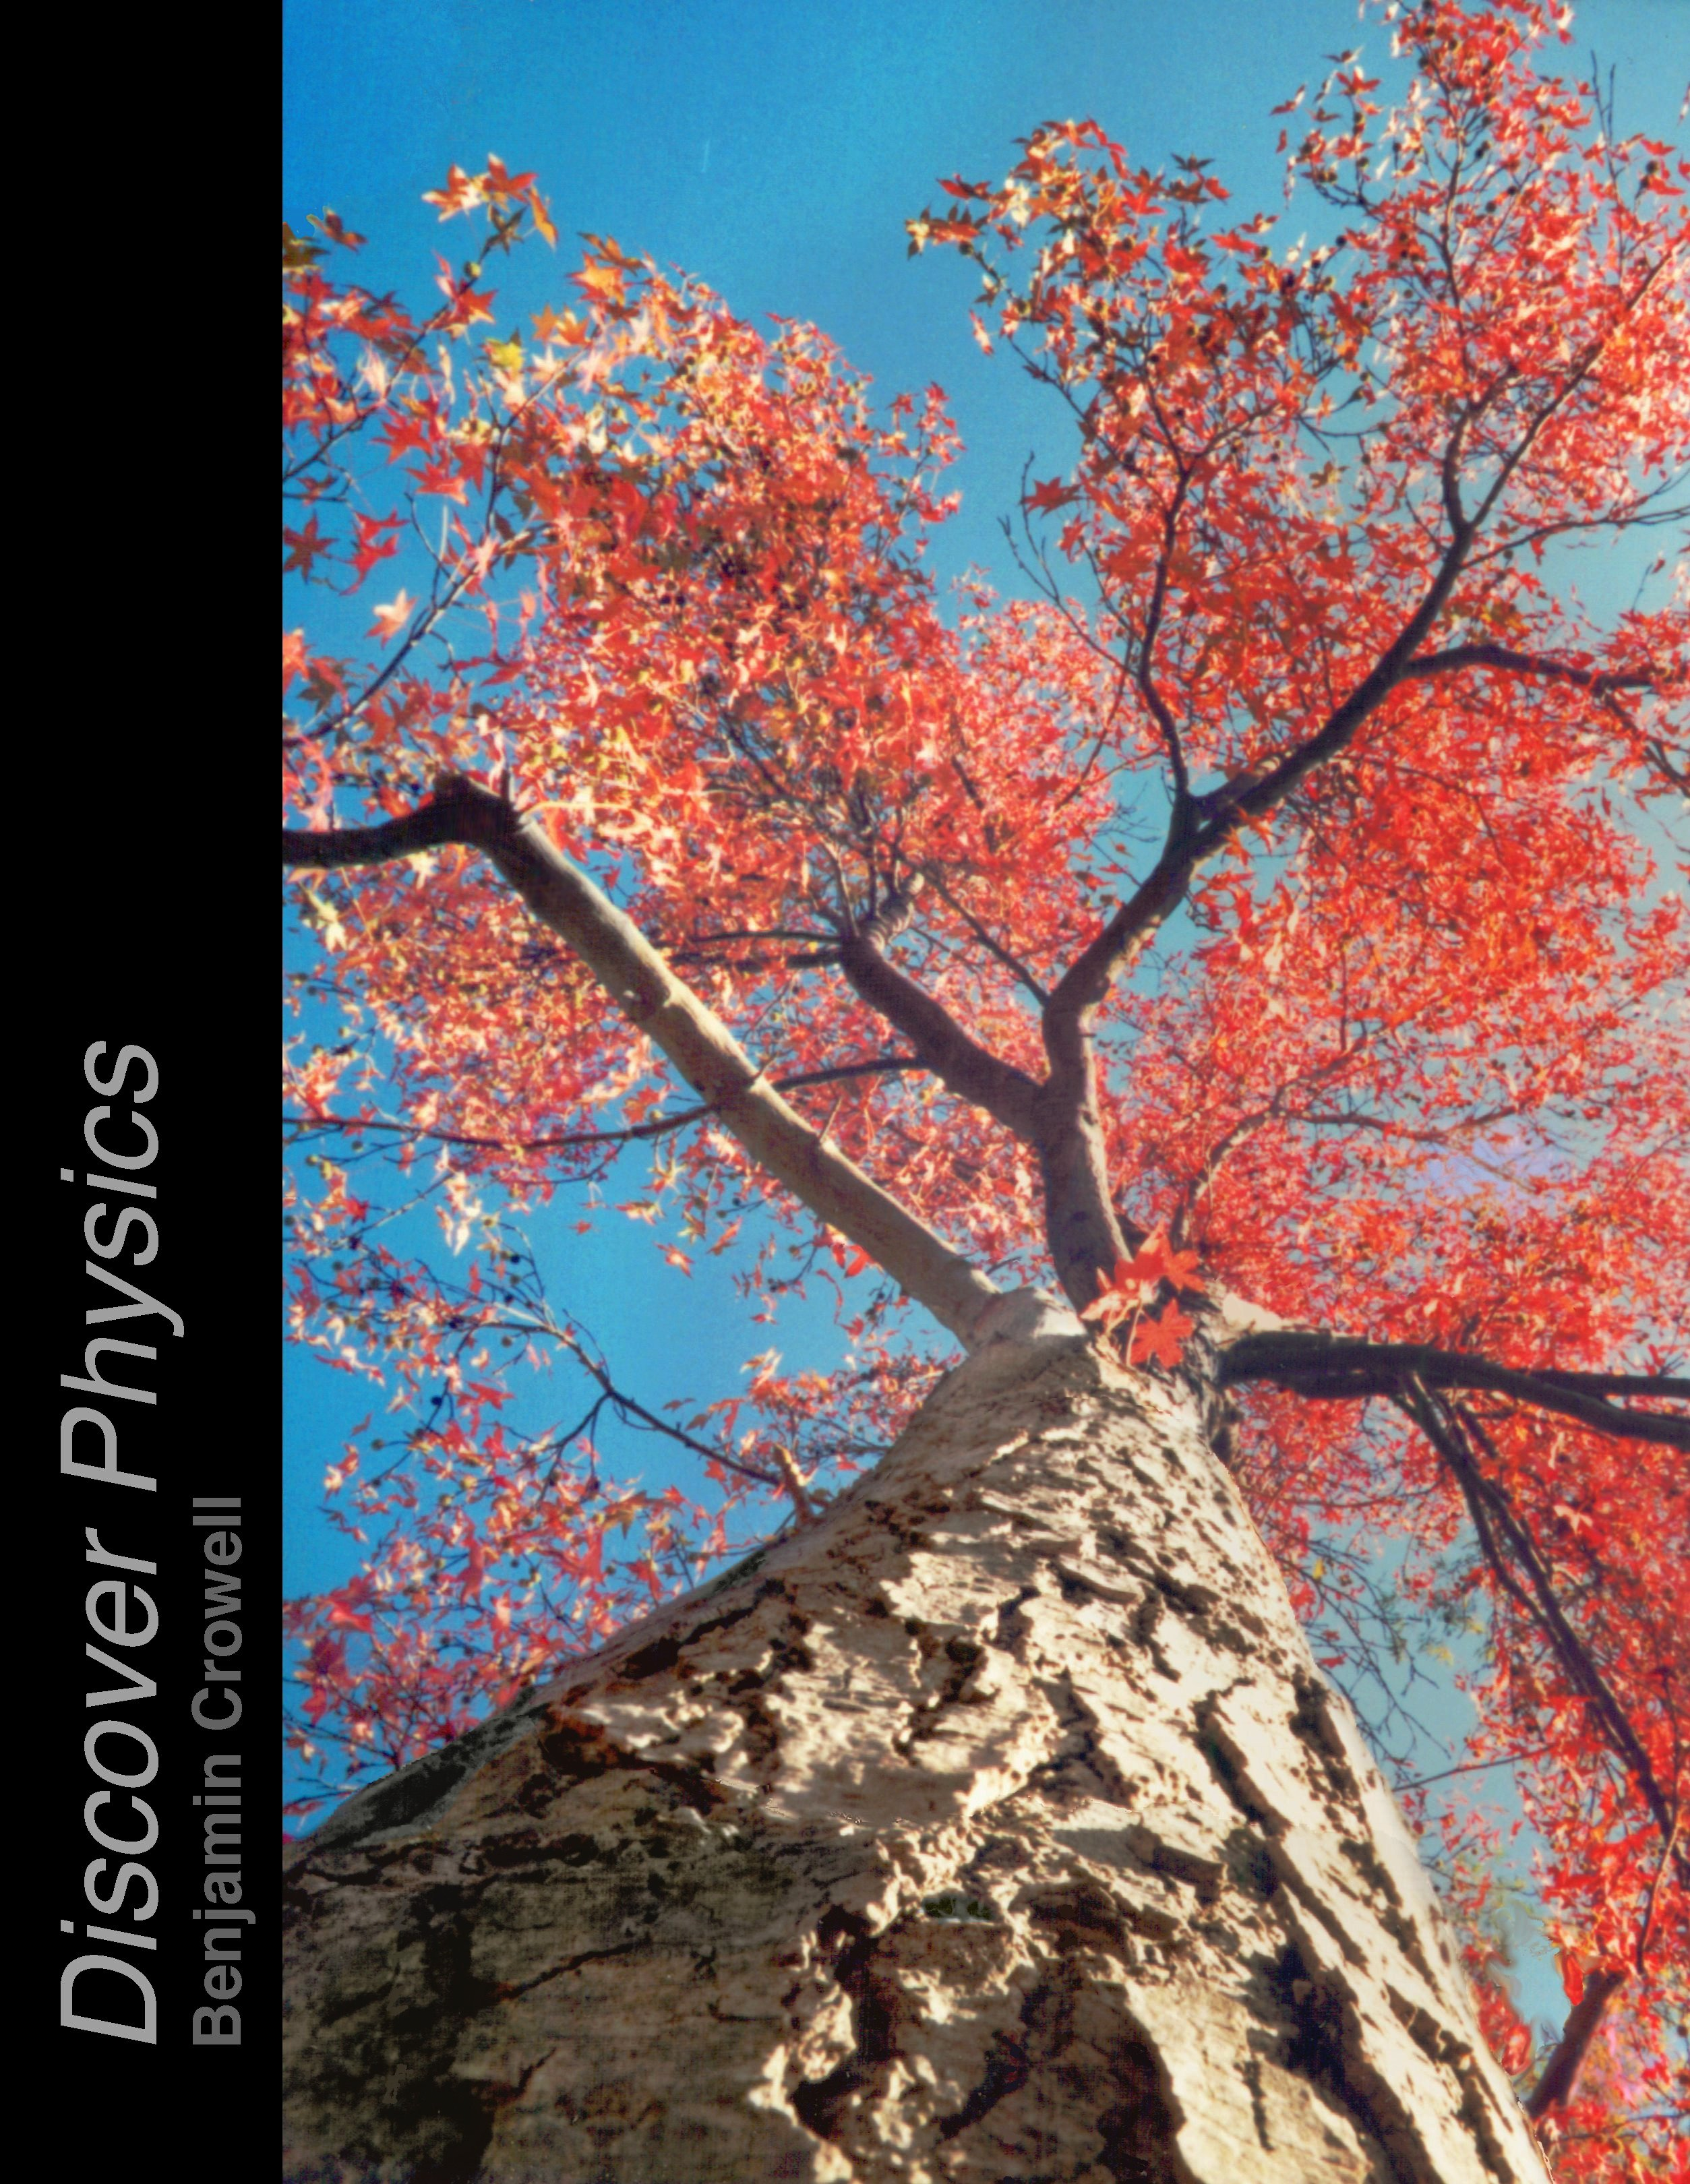
\includegraphics{\chapdir/figs/cover}\\
}
}%
\\



%based on a LaTeX copyright page by David Raymond
\thispagestyle{empty}

\vspace{100mm}

\noindent
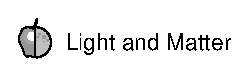
\includegraphics{ch00/figs/lmlogo}\\
Fullerton, California\\
www.lightandmatter.com

\vspace{20mm}
\noindent
Copyright \copyright  2002-2004 Benjamin Crowell\\
All rights reserved.

\vspace{20mm}
\noindent
rev. \today{}

\vspace{6mm}
\noindent
ISBN 0-9704670-8-7

\vspace{6mm}
\noindent
Permission is granted to copy, distribute and/or modify this
document under the terms of the Creative Commons Attribution
Share-Alike License, which can be found at creativecommons.org. The license
applies to the entire text of this book, plus all the illustrations
that are by Benjamin Crowell. All the illustrations are by Benjamin
Crowell except as noted in the photo credits or in parentheses
in the caption of the figure.
This book can be downloaded free of charge
from www.lightandmatter.com in a variety of formats,
including editable formats.

\yesiwantarabic
\nomarginlayout
\onecolumn\pagebreak[4]
\noindent\huge\bfseries\sffamily{}\vspace{50mm}

\hspace{2.5mm}\noindent{}Brief Contents

\vspace{2mm}\hbox{}

\noindent\mynormaltype\Large\sffamily{}\begin{tabular}{rl}
\ref{ch:symmetry} & The Rules of the Rules \quad \pageref{ch:symmetry}\\
\ref{ch:raymodel} & The Ray Model of Light \quad \pageref{ch:raymodel}\\
\ref{ch:images} & Images \quad \pageref{ch:images}\\
\ref{ch:energy} & Conservation of Mass and Energy \quad \pageref{ch:energy}\\
\ref{ch:momentum} & Conservation of Momentum \quad \pageref{ch:momentum}\\
\ref{ch:relativity} & Relativity \quad \pageref{ch:relativity}\\
\ref{ch:em} & Electricity and Magnetism \quad \pageref{ch:em}\\
\end{tabular}
\vfill
\mynormaltype

\pagebreak[4]

\vspace{0mm}
\begin{center}
\noindent\huge\bfseries\sffamily{}Contents\mynormaltype
\end{center}
\vspace{0mm}
\begin{multicols}{2}
  \tableofcontents
  \setcounter{unbalance}{0}
\end{multicols}
\normallayout\onecolumn

%========================= main matter =========================
\mainmatter
%-- I want the whole book numbered sequentially, arabic:
  \pagenumbering{arabic} 
  \addtocounter{page}{6} 
\parafmt
\myeqnspacing % Do this early and often, since it gets reset by \normalsize
%========================= chapters =========================
	\renewcommand{\chapdir}{ch01}\mychapterwithopener{dizzy}{Why do I get dizzy? Am I really spinning, or is the world
going around me? Humans are naturally curious about the universe they live in.}{The Rules of the Rules}\label{ch:symmetry}

Since birth, you've wanted to discover things. You started out by putting every available object in your
mouth. Later you began asking the grownups all those ``why'' questions. None of this makes you unique ---
humans are naturally curious animals. What's unusual is that you've decided
to take a physics course. There are easier ways to satisfy a science requirement, so evidently you're
one of those uncommon people who has retained the habit of curiosity into adulthood, and
you're willing to tackle a subject that requires sustained intellectual effort. Bravo!

A reward of curiosity is that as you learn more, things get simpler. ``Mommy, why do you have to go
to work?'' ``Daddy, why do you need keys to make the car go?'' ``Grandma, why can't I have that toy?''
Eventually you learned that questions like these, which as a child you thought to be unrelated,
were actually closely connected: they all had to do with capitalism and property. 
As a scientific example, William Jones\index{Jones, William} announced in 1786
the discovery that many languages previously thought
to be unrelated were actually connected. Jones realized, for example, that there was a relationship
between the words
``bhratar,'' ``phrater,'' ``frater,'' and ``brother,'' which mean the same thing
in Sanskrit, Greek, Latin, and English. Many apparently unrelated languages of Europe and
India could thus be brought under the same roof and understood in a simple way.
For an even more dramatic example, imagine trying to learn chemistry hundreds of years
ago, before anyone had discovered the periodic table or even the existence of atoms.\index{atoms}
Chemistry has gotten a lot simpler since then!\index{chemistry}

Sometimes the subject gets simpler, but it takes a while for the textbooks to catch up.
For hundreds of years after Hindu mathematicians incorporated negative numbers into
algebra, European texts still avoided them, which meant that students had to endure
a lot of confusing mumbo jumbo when it came to solving an equation like $x+7=0$.
Physics has been getting simpler, but most physics books still haven't caught up.
(Can you detect the sales pitch here?) The newer, simpler way of understanding physics
involves symmetry.

\pagebreak[4]

\mysection[0]{Symmetry}\index{symmetry}

\margup{-12mm}{\fig{noether}{Emmy Noether (1882-1935). The daughter of a prominent German mathematician, she did not show
any early precocity at mathematics --- as a teenager she was more interested in music and dancing.
She received her doctorate in 1907 and rapidly built a world-wide reputation, but the University
of G\"{o}ttingen refused to let her teach, and her colleague Hilbert had to advertise her courses in the
university's catalog under his own name. A long controversy ensued, with her opponents asking
what the country's soldiers would think when they returned home and were expected to learn
at the feet of a woman. Allowing her on the faculty would also mean letting her vote
in the academic senate. Said Hilbert, ``I do not see that the sex of the candidate is against
her admission as a privatdozent [instructor]. After all, the university senate is not a bathhouse.''
She was finally admitted to the faculty in 1919. A Jew, Noether fled Germany in 1933 and
joined the faculty at Bryn Mawr in the U.S.}}
%
The concept of symmetry goes back to ancient times, but the deep link between
physics and symmetry was 
discovered by Emmy Noether.\index{Noether, Emmy}
What do we mean by symmetry?\index{symmetry!defined}\index{symmetry!mirror}\index{symmetry!reflection}\index{symmetry!180-degree rotation}
Figure \figref{singlesymmetries} shows
two examples. The galaxy has a symmetry because it looks the same when
you turn your book upside-down. The orchid has a different type of symmetry: it looks the
same in a mirror. Reflection and 180-degree rotation are examples of transformations, i.e.,
changes in which every point in space is systematically relocated to some other
place. We say that a thing has symmetry when transforming it doesn't change it.
As shown in figure \figref{moresymmetries}, some objects have more
than one symmetry, although most have none.

\widefig{singlesymmetries}{Two types of symmetries.}
\widefig{moresymmetries}{Most object have no symmetries. Some have more than one.}

\selfcheck{playingcards}{What symmetry is possessed by most of the designs in a deck of cards? Why are
they designed that way?}

\begin{eg}{Palindromes}\index{palindromes}
A palindrome is a sentence that is the same when you reverse it: \\
I maim nine men in Saginaw; wan, I gas nine men in Miami.
\end{eg}

\pagebreak[4]

\dqheader
\begin{dq}
What symmetries does a human have? Consider internal features,
external features, and behavior. 
If you woke up one morning after having been reflected, would
you be able to tell? Would you die? What if the rest of the world
had been reflected as well?
\end{dq}

\vfill

\mysection[4]{A Preview of Noether's Theorem}\index{Noether's theorem!rough statement}

\margup{-150mm}{\fig{skaters}{What will happen when the two ice skaters push off from each
other?}
\spacebetweenfigs
\fig{checkersinitial}{The starting position in checkers.}
\spacebetweenfigs
\fig{checkerslater}{The board after two moves.}}
How does symmetry relate to physics? Long before Noether's work, it had been
recognized that some physical systems had symmetry, and their symmetries could
be helpful for predicting their behavior. If the skaters in
figure \figref{skaters} have equal masses, symmetry tells us that they will
move away from each other at equal speeds after they push off. 
The one on the right looks bigger, however, so the symmetry argument doesn't
quite work. If you look at the world around you, you will see many approximate
examples of symmetry, but none that are perfect. Most things have
no symmetry at all. Until Noether's work, that was the whole story.
Symmetry was on the sidelines of physics.\label{original-skaters}

Noether's approach was different. The universe is made out of particles, and
these particles are like the players on a soccer field
or the pieces on a checkerboard. The arrangement of the players on the
soccer field normally has no symmetry at all. The symmetry is in the rules:
the rules apply equally to both sides. Likewise, the physical arrangement
of the checkers on the board in figure \figref{checkersinitial} has
180-degree rotation symmetry, but this is spoiled in figure \figref{checkerslater}
after a couple of moves. We don't care about the asymmetry of the pieces.
In Noether's approach, what's important is the symmetry of the rules.
If we think of the checkerboard as a little universe, then these rules are like
the laws of physics, and their symmetry allows us to predict certain things
about how the universe will behave. For instance, suppose we balanced the board
carefully on a knife edge running from left to right below its centerline. The
position in figure \figref{checkersinitial} balances, and so does the one
in figure \figref{checkerslater}. The rules required both red and black to
move one piece diagonally forward one step, so we were guaranteed that after
each side had made one move, the setup would balance again.\footnote{This
symmetry won't continue indefinitely, because at some point one player will
jump one of the other player's pieces, or get a king and make a backwards
move. That just shows that a game like checkers is an imperfect metaphor for
the laws of physics. The particles in the universe don't take turns moving,
so we don't have situations where one particle sits still while another
one ``jumps'' it. It is possible for a particle of matter and a particle of
antimatter to annihilate one another --- the process is probably occurring in
the room you're in right now, due to natural radioactivity --- but neither particle
exists afterwards, so the symmetry is more perfect than in checkers.
The laws of physics are also deterministic; there is
no choice involved, as in a game.}

Noether's greatest achievement was a principle known as Noether's theorem.
We are not yet ready to state Noether's theorem exactly, but roughly speaking,
here's what it says: The laws of physics have to be the way they are because
of symmetry.

\mysection[0]{What Are The Symmetries?}
What are the actual symmetries of the laws of physics? It's tempting to try to
determine them by pure reason, or by aesthetic arguments. Why, for example, would
God have chosen laws of physics that didn't treat right and left the same way? That
would seem ugly. The trouble with this approach is that it doesn't work.

For example, prehistoric peoples observed the rising and setting of the sun, the moon,
the stars, and the four naked-eye planets. They all appeared to be going in circles,
and a circle is a very symmetric shape: it remains the same under rotation through
any angle at all. It became accepted dogma among the ancient astronomers that these
heavenly bodies were attached to spinning crystal spheres. When careful observations
showed that the motion of the planets wasn't quite circular, they patched things up by imagining
smaller crystal spheres riding on the big ones. This bias toward spheres and circles
was hard to shake because the symmetry of the shapes was so appealing. The astronomer
Johannes Kepler (1571-1630) inherited from his predecessor Tycho Brahe (1546-1601)\index{Kepler, Johannes}\index{Brahe, Tycho}
a set of the best observations ever made of the motions of the planets. Kepler
labored for years trying to make up a set of spheres riding on spheres that would
fit the data, but because the data were so accurate, he finally realized what nobody
could have known based on the older, less precise observations: it simply wasn't
possible. Reluctantly, Kepler gave up his mystical reverence for the symmetry of the
circle. He eventually realized that the planets' orbits were ovals of a specific
mathematical type called an ellipse. The new observations showed that the laws of physics
were less symmetric than everyone had believed.

\margup{-145mm}{\fig{startrails}{Due to the earth's rotation, the stars appear to go in circles. In this
time-exposure photograph, each star makes an arc.}
\spacebetweenfigs
\fig{checkerstranslational}{A chess board has a kind of translational symmetry: it
looks the same if we slide it one square over and one square up.}
\spacebetweenfigs
\fig{sodastraw}{The soda straw has translational symmetry. The flea exploring along its length
doesn't see anything different from one location to another.}
}
Sometimes experiments show that physics is \emph{more} symmetric than expected. One good
example of this is translational symmetry.\index{symmetry!translational} A translation is a type of transformation
in which we slide everything without rotating it, as in figure \figref{checkerstranslational},
where we can slide the chess board so that the black squares are again in the places previously
occupied by black squares.\footnote{The chess board lacks complete translational symmetry
because it has edges. As far as we know, the laws of physics don't specify that there are
edges to the universe beyond which nothing can go. However, this is different from the
question of whether the universe has infinite volume. We can easily make a chessboard that
is finite but has no edges. We simply wrap the right and left edges around to form a tube,
and then bend the tube into a doughnut. We still don't know with certainty whether the
universe is finite or infinite, although the latest data seem to show it's infinite.
Einstein's theory of general relativity allows either possibility.}
The ancient Greek philosopher Aristotle\index{Aristotle} believed that the rules were different in some
parts of the universe than in others. In modern terminology, we say that he didn't
believe in translational symmetry. When you drop a rock, it falls. Aristotle explained
this by saying that the rock was trying to go back to its ``natural'' place, which is
the surface of the earth. He applied the same kind of explanation to rising smoke: it rises
because it wants to go to its own natural place, which is higher up. In Aristotle's
theory, different parts of the universe had their own special characteristics.
Only after an interval of two thousand years was the true translational symmetry of
the laws of physics uncovered by Isaac Newton.\index{Newton, Isaac} In Newton's theory of gravity,
a rock falls because every atom in the universe is attracted to every other atom.
The rock's atoms are attracted to the planet earth's atoms. We don't prefer Newton's
version just because it sounds better. Aristotle was proved wrong by
experiments. The original evidence was indirect, but we have more straightforward
proof now. If Aristotle had been right, the huge boulder in figure \figref{schmidtonmoon}
would long since have fallen to its ``natural'' place on the surface of our planet
(and so would the astronaut!).\label{space-translation-symmetry}

\widefigsidecaption{schmidtonmoon}{Astronaut Harrison Schmidt on the moon in 1972.}

Translational symmetry is also deeply embedded in the way we practice the scientific
method. One of the assumptions of the scientific method is that experiments should
be reproducible. For example, a group at Berkeley recently claimed to have produced
three atoms of a new element, with atomic number 118. Other labs, however, were
unable to reproduce the experiment, and eventually suspicious members of the Berkeley
team checked and found that one of their own scientists had fabricated the data.
Although the episode (and another case of fraud at Bell Laboratories around the same
time) caused considerable editorializing about what might be wrong with the
scientific profession, I see it as a textbook example of how the scientific method
is supposed to work, since the fraud was eventually discovered. A basic assumption
here is that scientists in different places should be able to get the same
results. If translational symmetry was violated, then the results might be different
because the laws of physics were different in different places. The assumption of
translational symmetry is so deeply ingrained that normally it doesn't
even occur to us that we were making it. When engineers design a space probe to
go to Mars, they don't even stop to ask themselves whether the laws of physics
are the same on Mars as on earth.

\dqheader

\begin{dq}\label{dq:ozma}
Imagine that you establish two-way radio communication with aliens. You laboriously
teach each other your languages, e.g., by sending two beeps followed by the word
``two.'' However, neither of
you is able to figure out exactly where the other's planet is, and you can't
come up with any celestial landmarks that you both recognize. Can you communicate
the definition of the terms ``right'' and ``left'' to them? The wonderful popular science
writer Martin Gardner proposes calling this the ``Ozma problem.'' (The name comes
from the Ozma project, which was the first serious attempt to detect signals from
aliens using radio telescopes. The Ozma project was in turn named after a character
in one of L. Frank Baum's Oz stories.) In general, every
symmetry of the laws of physics can be stated as an Ozma problem.\index{Ozma problem!for left and right}
\end{dq}

%===============================================================================
%===============================================================================

\vfill\pagebreak[4]
\noindent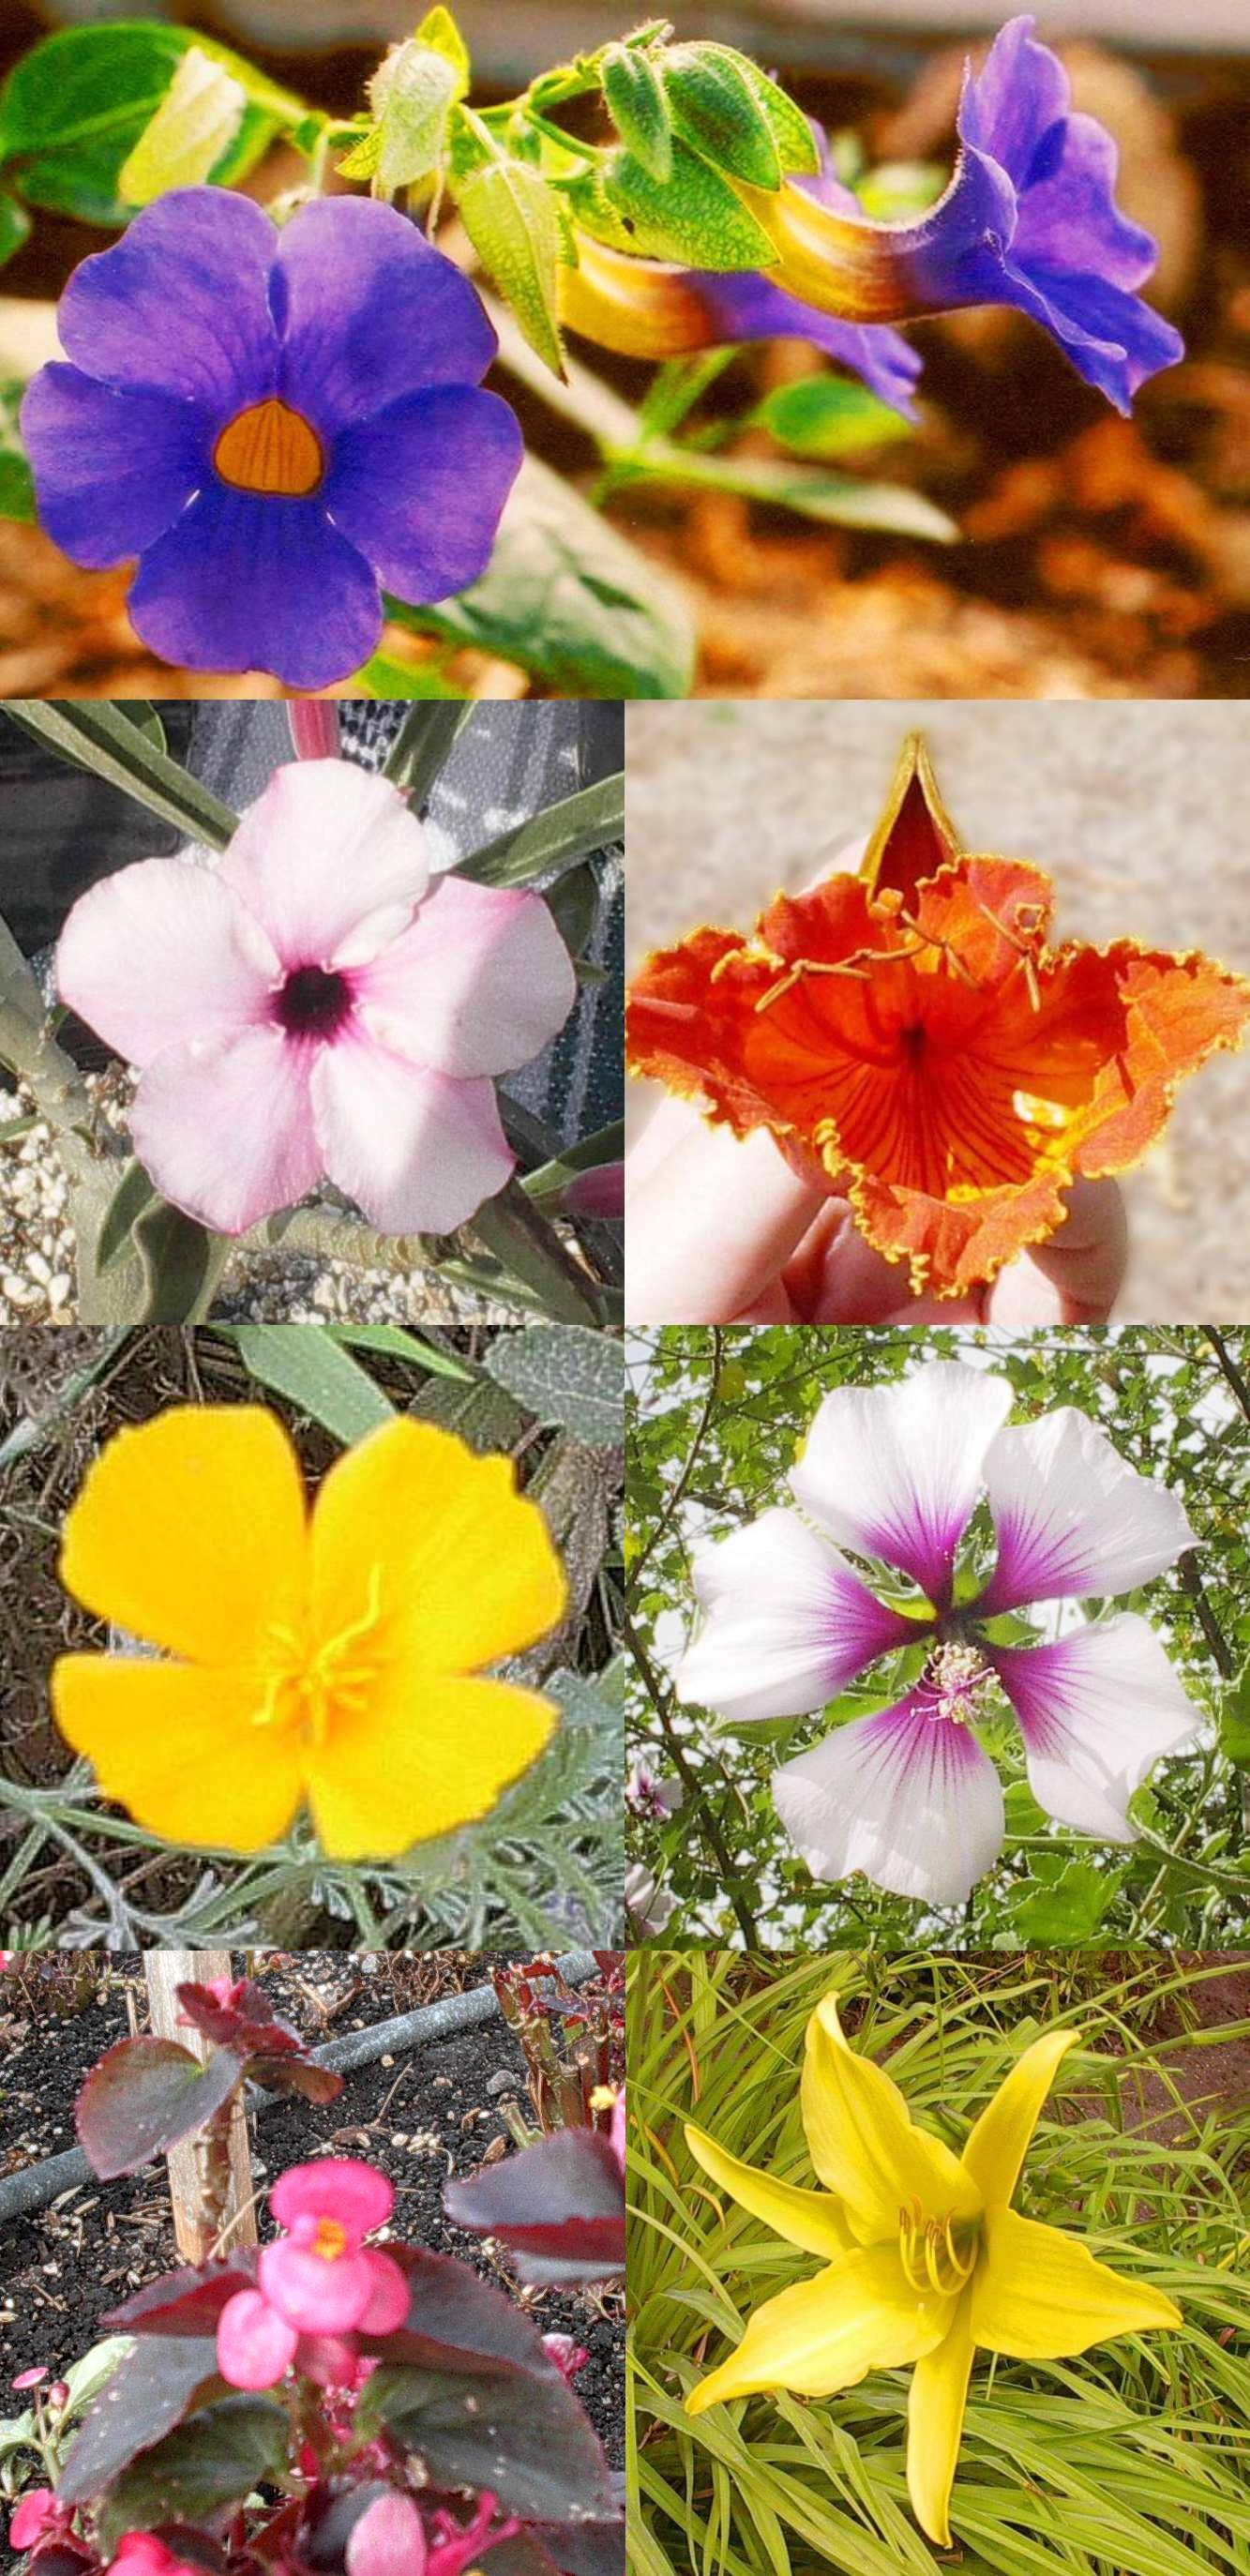
\includegraphics[width=100mm]{\chapdir/figs/flowers}\label{fig:flowers}
\marg{%
\raisebox{100mm}[0mm][0mm]{%
\parbox{52mm}{
\noindent\formatlikecaption{These flowers are referred to in homework problems
\ref{hw:flowersa} and \ref{hw:flowersb}.}\\
\noindent\includegraphics[width=52mm]{\chapdir/figs/flowernames}
}}}

\vfill\pagebreak[4]
\begin{hwsection}

\hwnote{%
Problems \ref{hw:flowersa} and \ref{hw:flowersb} refer to the photos of flowers on
page \pageref{fig:flowers}. Since the flowers are living things, they don't have
exact, perfect mathematical symmetry. Just think in terms of approximate symmetries.
}

\begin{hw}{flowersa}
(a) Which of the flowers shown in the photos have reflection symmetry but not 180-degree
rotation symmetry? \hwendpart
(b) Which have 180-degree rotation symmetry but not reflection symmetry?\hwendpart
(c) Which have both\hwendpart
(d) Which have neither?\hwendpart
Note that in flowers 1 and 2, the lobes of
the petals overlap in a clockwise or counterclockwise screw pattern.
You can tell from the photo that flower 1 has a curved tube. Flower 2 doesn't have a curved tube.
\end{hw}

\begin{hw}{flowersb}
In the text, I've only discussed rotational symmetry with an angle of 180 degrees.
Some of the flowers in the photos have symmetry with respect to other angles. Discuss
these.
\end{hw}

\begin{hw}[2]{flowersresearch}
The following are questions about the symmetries of plants that you can try to
answer by collecting data at an arboretum, nursery, botanical garden, or florist.
(You could also websurf, but it wouldn't be as enjoyable.) You probably won't be
able to answer all of them. You can't do this problem without actually going out
and collecting detailed data; you'll have to turn in the data (drawings, notes
on which plants you looked at, etc.) and then base your conclusions on your data.
\begin{itemize}
 \item[] Symmetry of flowers is an easy way to classify plants. Is it also a good way?
  To be a good way, it should correspond to evolutionary relationships, and it
  should therefore correlate with other features of plants. Another feature
  that's easy to check is leaf structure: are the fibers in the leaves all
  parallel (e.g., grass), or do they branch out (e.g., a maple). Does leaf structure
  seem to correlate at all with flower symmetry?
 \item[] The photos on page \pageref{fig:flowers} include some flowers whose petals or
  petal-lobes overlap in a pattern like a clockwise or counterclockwise screw. When this
  happens, how systematic is the pattern of overlapping? Do you observe right-handed and
  left-handed screw-patterns in different flowers on the same plant? In different plants
  that are genetically identical (e.g., grown from cuttings from the same parent) but
  have been exposed to different environments? In genetically different plants of the same
  species?
 \item[] Can you find any plants in which the arrangement of the leaves follows a definite
  pattern, but lacks reflection symmetry?
\end{itemize}
\end{hw}

\begin{hw}{noethernotobjects}
Noether's theorem refers to symmetries of the laws of physics, not symmetries of
objects.
Which of the following do you think could qualify as a law of physics, and which
are mere facts about objects? In other words, which ones are \emph{not} true
in some situations, at some times, on different planets, etc? They are all true
where I live!
\begin{enumerate}
 \item The sun rises in the east and sets in the west.
 \item High tide occurs when the moon is overhead or underfoot, and low tide
   when it's on the horizon.
 \item Inheritance works through genes, so an acquired trait can't be inherited.
 \item In a chemical reaction, if you weigh all the products, the total is the same
   as what you started with.
 \item A gas compressed to half its original volume will have twice its original pressure
	(assuming the temperature is the same).
\end{enumerate}
In each case, explain your reasoning.
\end{hw}

\begin{hw}{ninetydegreerotation}
If an object has 90-degree rotation symmetry, what other symmetries must it have as well?\\
\end{hw}

\begin{hw}{onethirtyfivedegreerotation}
Someone describes an object that has symmetry under 135-degree rotation (3/8 of a circle).
What's a simpler way to describe the same symmetry? (Hint: Draw a design on a piece of
paper, then trace it onto another piece of paper. Rotate the top piece of paper, then
copy the new design. Keep going. What happens?)
\end{hw}

\begin{hw}{oneeightyandreflection}
(a) Give an example of an object that has 180-degree rotation symmetry, and also has reflection
symmetry. \\
(b) Give an example with symmetry under 180-degree rotation, but \emph{not} under reflection.
\end{hw}

\begin{hw}{elephant}
Suppose someone tells you that the reason the Ozma problem for left and right is
difficult is because you can't get together with the aliens and show them what you're
referring to. Is this correct? How is this different from trying to describe an elephant
over the radio to someone who's never seen an elephant or a picture of one?
\end{hw}

\end{hwsection}


%========================================== labs ===============================================

\begin{lab}{Scaling}\index{scaling}

\apparatus
\equip{paper and card stock}\\
\equip{ruler}\\
\equip{scissors}

\goal{Find out whether the laws of physics have scaling symmetry.}

\labintroduction

From Gulliver to Godzilla, people have always been fascinated with
scaling.\index{Gulliver}\index{Godzilla}\index{Galileo}
Gulliver's large size relative to the Lilliputians obviously had some strong
implications for the story. But is it only \emph{relative} size that matters?
In other words, if you woke up tomorrow, and both you and your house had been
shrunk to half their previous size, would you be able to tell before stepping
out the door? Galileo was the first to realize that this type of question was
important, and that the answer could only be found by experiments, not by looking
in dusty old books. In his book \emph{The Two New Sciences}, he illustrated
the question using the idea of a long wooden plank, supported at one end, that
was just barely strong enough to keep from breaking due to gravity. The testable
question he then posed was whether this just-barely-strong-enough plank would
still have the just-barely-strong-enough property if you scaled it up or down,
i.e., if you multiplied all its dimensions --- length, width, and height ---
by the same number.

\labfigcaption{lab-galileo-board}{Galileo's illustration of his idea.}

You're going to test the same thing in lab, using the slightly less picturesque
apparatus shown in the photo: strips of paper. The paper bends rather than breaking,
but by looking at how much it droops, you can see how able it is to support its
own weight.
The idea is to cut out different
strips of paper that have the same proportions, but different sizes. If the
laws of physics are symmetric with respect to scaling, then they should all
droop the same amount. Note that it's important to scale all three dimensions
consistently, so you have to use thicker paper for your bigger strips and
thinner paper for the smaller ones. Paper only comes in certain thicknesses,
so you'll have to determine the widths and lengths of your strips based on
the thicknesses of the different types of paper you have to work with. 
In the U.S., some common thicknesses of paper and card-stock are
78, 90, 145, and 200 grams per square meter.\footnote{A student at Ohlone College,
using the same brand of paper I use at Fullerton College,
noticed that the numbers given on the packaging in units of pounds
do not correspond at all closely to the thickness or weight of the paper. The
densities are also a little different, but not too different, so it's not such
a bad assumption to assume that weight relates directly to thickness.}
We'll assume that these numbers also correspond
to thicknesses. For instance, 200 is about 2.56 times greater than 78, so the
strip you cut from the heaviest card stock should have a length and
width that are 2.56 times greater than the corresponding dimensions of
the strip you make from the lightest paper.

\labfig{lab-paper-strip}

\labsection{To Think About Before Lab}

1. If the laws of physics are symmetric with respect to
scaling, would each strip droop by the same number of centimeters,
or by the same angle? In other words, how should you choose to
define and measure the ``droop?''

2. If you find that all the strips have the same droop,
that's evidence for scaling symmetry, and if you find that they droop
different amounts, that's evidence against it. Would either observation
amount to a proof? What if some experiments showed scaling symmetry and
others didn't?


\end{lab}


%========================================== self-check answers ===============================================
\startscanswers{ch:symmetry}
\scanshdr{playingcards}{They have 180-degree rotation symmetry. They're designed that way
so that when you pick up your hand, it doesn't matter which way each card is turned.}

%========================================== toc decoration ===============================================
\addtocontents{toc}{\protect\figureintoc{schmidtonmoon}}
% 
	\renewcommand{\chapdir}{ch02}\mychapter{The Ray Model of Light}\label{ch:raymodel}\index{light!ray model}

\mysection[0]{Rays Don't Rust}

If you look at the winter night sky on a clear, moonless night far from any city
lights, something strange will soon catch your eye. Near the constellation of Andromeda\index{Andromeda galaxy}
is a little white smudge. What is it? You can easily convince yourself that it's
not a cloud, because it moves along with the stars as they rise and set. What you're
seeing is the Andromeda galaxy, a fantastically distant group of stars very similar
to our own Milky Way.%
\footnote{If you're in the
southern hemisphere, you have a more scenic sky than we in the north do, but
unfortunately you can't see any naked-eye objects that are as distant as the
Andromeda galaxy. You can enjoy the Magellanic Clouds and the Omega Centauri
cluster, but they're an order of magnitude closer.}
We can see individual stars within the Milky Way galaxy because
we're inside it, but the Andromeda galaxy looks like a fuzzy patch because we can't
make out its individual stars.
The vast distance to the Andromeda galaxy is hard to fathom, and it won't help
you to imagine it if I tell you the number of kilometers is 2 followed by 
19 zeroes.
Think of it like this: if the stars in our own galaxy were as close together
as the hairs on your skin, the Andromeda galaxy would be thousands of kilometers
away.

\margup{-75mm}{\fig{andromedamap}{How to locate the Andromeda galaxy.}}
The light had a long journey to get to your eyeball! A well-maintained car might
survive long enough to accumulate a million kilometers on its odometer, but
by that time it would be a rickety old rust-bucket, and the distance it had covered would
still only amount to a fraction of a billionth of a billionth of the distance
we're talking about. Light doesn't rust. A car's tracks can't
go on forever, but the trail of a light beam can. We call this
trail a ``ray.''

\mysection[0]{Time-Reversal Symmetry}\index{symmetry!time-reversal}

The neverending motion of a light ray is surprising compared
with the behavior of everyday objects, but in a way it makes sense. A car is
a complex system with hundreds of moving parts. Those parts can break,
or wear down due to friction. Each part is itself made of atoms, which can
do chemical reactions such as rusting. 
Light, however, is fundamental: as far as we know, it isn't
made of anything else. 
My wife's car has a dent in it that preserves the record of the time she
got rear-ended last year. As time goes on, a car accumulates more and more history.
Not so with a light ray. Since a light ray carries no history, there is no way
to distinguish its past from its future. Similarly, some brain-injured people
are unable to form long-term memories. To you and me, yesterday is different
from tomorrow because we can't remember tomorrow, but to them there is no such
distinction.

Experiments --- including some of the experiments you're going to do in this
course --- show that the laws of physics governing light rays are perfectly
symmetric with respect to past and future. If a light ray can go from A to
B, then it's also possible for a ray to go from B to A. I remember as a child
thinking that if I covered my eyes, my mommy couldn't see me. I was almost
right: if I couldn't see her eyes, she couldn't see mine. 

\begin{eg}{Why light rays don't stop}\label{eg:tiredlight}
Once the experimental evidence convinces us of time-reversal symmetry, it's
easy to prove that light rays never get tired and stop moving. Suppose
some light was headed our way from the Andromeda galaxy, but it
stopped somewhere along the way and never went any farther. Its trail,
which we call the ``ray,'' would be a straight line ending at that
point in empty space. Now suppose we send a film crew along in a space ship to document
the voyage, and we ask them to play back the video for us, but backwards.
Time is reversed. The narration is backwards. Clocks on the wall go counterclockwise.
In the reversed documentary, how does the light ray behave? At the beginning
(which is really the end), the light ray doesn't exist. Then, at some random moment
in time, the ray springs into existence, and starts heading back towards the
Andromeda galaxy. In this backwards version of the documentary, the light ray
is not behaving the way light rays are supposed to. Light doesn't just appear
out of nowhere in the middle of empty space for no reason. (If it did, it would
violate rotational symmetry, because there would be no physical reason why this
out-of-nowhere light ray would be moving in one direction rather than another.)
Since the backwards video is impossible, and all our accumulated data have shown that
light's behavior has time-reversal symmetry, we conclude that the forward video is
also impossible. Thus, it is not possible for a light ray to stop in the middle of empty
space.
\end{eg}

\marg{\fig{apollomirror}{The mirror left on the moon by the Apollo 11 astronauts.}}
\begin{eg}{The Apollo lunar ranging experiment}\label{eg:lunarranging}
In 1969, the Apollo 11 astronauts made the first crewed landing on the moon, and
while they were there they placed a mirror on the lunar surface. Astronomers
on earth then directed a laser beam at the landing site. The beam was reflected
by the mirror, and retraced its own path back to the earth, allowing the distance
to the moon to be measured extremely accurately (which turns out to provide important
information about the earth-moon system). Based on time-reversal symmetry,
we know that if the reflection is a 180-degree
turn, the reflected ray will behave in the same way as the outgoing one, and retrace
the same path. (Figure \figref{cornerreflector} on page
\pageref{fig:cornerreflector} explains the clever trick used to make sure the reflection
would be a 180-degree turn, without having to align the mirror perfectly.)
\end{eg}

\pagebreak[4]

\begin{eg}{Looking the wrong way through your glasses}
If you take off your glasses, turn them around, and look through them the other
way, they still work. This is essentially a demonstration of time-reversal
symmetry, although an imperfect one. It's imperfect because you're not
time-reversing the entire path of the rays. Instead of passing first through
the front surface of the lenses, then through the back surface, and then
through the surface of your eye, the rays are now going through the three
surfaces in a different order. For this reason, you'll notice that things look
a little distorted with your glasses reversed. To make a perfect example of
time-reversal, you'd have to have a little lamp inside your eyeball!
\end{eg}

If light never gets tired, why is it that I usually can't see the mountains from
my home in Southern California? They're far away, but if light never stops, why
should that matter? It's not that light just naturally stops after traveling
a certain distance, because I can easily see the sun, moon, and stars from my house,
and they're much farther away than the mountains. The difference is that my line
of sight to the mountains cuts through many miles of pollution and natural haze.
The time-reversal argument in example \ref{eg:tiredlight} depended on the assumption that the
light ray was traveling through empty space. If a light ray starts toward me from the
mountains, but hits a particle of
soot in the air, then the time-reversed story is perfectly reasonable: a particle
of soot emitted a ray of light, which hit the mountains.

\dqheader
\begin{dq}
If you watch a time-reversed soccer game, are the players still obeying the rules?
\end{dq}

\pagebreak[4]

\mysection[0]{Applications}
\begin{envsubsection}{The inverse-square law}\index{inverse-square law}
Yet another objection is that a distant candle appears dim. Why is this, if not
because the light is getting tired on the way to us? Likewise, our sun is just
a star like any other star, but it appears much brighter because it's so much
closer to us. Why are the other stars so dim if not because their light wears out?
It's not that the light rays are stopping, it's that they're
getting spread out more thinly. The light comes out of the source in all directions, and if you're
very far away, only a tiny percentage of the light will go into your eye. (If all the
light from a star went into your eye, you'd be in trouble.)


\widefigsidecaption[c]{inversesquare}{The light is four times dimmer at twice the distance.}

Figure \figref{inversesquare} shows what happens if you double your distance from the source. The
light from the flame spreads out in all directions. We pick four
representative rays from among those
that happen to pass through the nearer square. Of these four,
only one passes through the square of equal area at twice the distance. If the
two equal-area squares were people's eyes, then only one fourth of the light would
go into the more distant person's eye.


Another way
of thinking about it is that the light that passed through the first square spreads
out and makes a bigger square; at double the distance, the square is twice as wide and
twice as tall, so its area is $2\times2=4$ times greater. The same light has been spread
out over four times the area.

In general,
the rule works like this:
\begin{align*}
	\text{distance}\times2 &\Rightarrow \text{brightness}\times\frac{1}{4}\\
	\text{distance}\times3 &\Rightarrow \text{brightness}\times\frac{1}{9}\\
	\text{distance}\times4 &\Rightarrow \text{brightness}\times\frac{1}{16}
\end{align*}
To get the 4, we multiplied 2 by itself, 9 came from multiplying 3 by itself, and so on.
Multiplying a number by itself is called squaring it, and dividing one by a number
is called inverting it, so a relationship like this is known as an inverse square law.
Inverse square laws are very common in physics: they occur whenever something is spreading
out in all directions from a point.

\selfcheck{candlefivetimes}{%
Alice is one meter from the candle, while Bob is at a distance of five meters.
How many times dimmer is the light at Bob's location?%
}

\begin{eg}{An example with sound}
\egquestion Four castaways are adrift in an open boat, and are yelling to try to attract the
attention of passing ships. If all four of them yell at once, how much is their range
increased compared to the range they would have if they took turns yelling one at a time?\\
\eganswer This is an example involving sound. Although sound isn't the same as light,
it does spread out in all directions from a source, so it obeys the inverse-square
law. In the previous examples, we knew the distance and wanted to find the intensity
(brightness). Here, we know about the intensity (loudness), and we want to find out
about the distance. Rather than taking a number and multiplying it by itself to find the
answer, we need to reverse the process, and find the number that, when multiplied by
itself, gives four. In other words, we're computing the square root of four, which is
two. They will double their range, not quadruple it. 
\end{eg}

\begin{eg}{Astronomical distance scales}\label{eg:alphacdistance}
The nearest star, Alpha Centauri,\footnote{Sticklers will note that the nearest star
is really our own sun, and the second nearest is the burned-out cinder
known as Proxima Centauri, which is Alpha Centauri's close companion.}
is about 10,000,000,000,000,000 times dimmer than our sun when viewed from
our planet. If we assume that Alpha Centauri's true brightness is roughly the same
as that of our own sun, then we can find the distance to Alpha Centauri by
taking the square root of this number. Alpha Centauri's distance from us
is equal to about 100,000,000 times our distance from the sun.
\end{eg}

\margup{-100mm}{\fig{diaphragm}{The same lens is shown with its diaphragm set to three different
apertures.}}
\begin{eg}{Pupils and camera diaphragms}
In bright sunlight, your pupils contract to admit less light. At night they dilate,
becoming bigger ``light buckets.''
Your perception of brightness depends not only on the true brightness of the source
and your distance from it, but also on how much area your pupils present to the light.
Cameras have a similar mechanism, which is easy to see if you detach the lens
and its housing from the body of the camera, as shown in the figure. Here, the diameter of
the largest aperture is about ten times greater than that of the smallest aperture.
Making a circle ten times greater in radius increases its area by a factor of 100, so
the light-gathering power of the camera becomes 100 times greater. (Many people expect
that the area would only be ten times greater, but if you start drawing copies of the
small circle inside the large circle, you'll see that ten are not nearly enough to
fill in the entire area of the larger circle. Both the width and the height of the
bigger circle are ten times greater, so its area is 100 times greater.)
\end{eg}
\end{envsubsection}
%
\begin{envsubsection}{Parallax}\index{parallax}
Example \ref{eg:alphacdistance} on page \pageref{eg:alphacdistance} showed how we
can use brightness to determine distance, but your eye-brain system has a different method.
Right now, you can tell how far away this page is from your eyes. This sense of
depth perception comes from the fact that your two eyes show you the same scene
from two different perspectives. If you wink one eye and then the other, the page will
appear to shift back and forth a little.

\widefig{parallax}{At double the distance, the parallax angle is approximately halved.}
If you were looking at a fly on the bridge
of your nose, there would be an angle of nearly $180\degunit$ between the ray that
went into your left eye and the one that went into your right. Your brain would know
that this large angle implied a very small distance. This is called the parallax
angle. Objects at greater distances have smaller parallax angles, and when the angles
are small, it's a good approximation to say that the angle is inversely proportional
to the distance. In figure \figref{parallax}, the parallax angle is almost exactly
cut in half when the person moves twice as far away.

Parallax can be observed in other ways than with a pair of eyeballs.
As a child, you noticed that when you walked around on a moonlit evening,
the moon seemed to follow you. The moon wasn't really following you, and this isn't
even a special property of the moon. It's just that as you walk, you expect to observe
a parallax angle between the same scene viewed from different positions of your whole head.
Very distant objects, including those on the Earth's surface, have parallax
angles too small to notice by walking back and forth. In general, rays coming from
a very distant object are nearly parallel.

If your baseline is long enough, however, the small parallaxes of even very distant objects
may be detectable. In the nineteenth century, nobody knew how tall the Himalayas were,
or exactly where their peaks were on a map, and the Andes were generally believed to be the
tallest mountains in the world. The Himalayas had never been climbed, and could only be viewed
from a distance. From down on the plains of India, there was no way to tell whether they were
very tall mountains very far away, or relatively low ones that were much closer. British
surveyor George Everest finally established their true distance, and astounding height,
by observing the same peaks through a telescope from different locations far apart.

An even more spectacular feat of measurement was carried out by Hipparchus over\index{Hipparchus}\index{moon!distance to}
twenty-one centuries ago. By measuring the parallax of the moon as observed from
Alexandria and the Hellespont, he determined its distance to be about 90 times
the radius of the earth.\footnote{The reason this was
a hard measurement was that accurate clocks hadn't been invented, so there was no
easy way to synchronize the two observations, and the desired effect would be masked
by the apparent motion of the moon across the sky as it rose and set. Hipparchus's trick
was to do the measurement during a solar eclipse, so that people at both locations
would know they were in sync.}\label{hipparchusmoondistance}

The earth circles the sun, \figref{stellarparallax}, and we can therefore determine the distances to a few
hundred of the nearest stars by making observations six months apart, so that the
baseline for the parallax measurement is the diameter of the earth's orbit. For these
stars, the distances derived from parallax can be checked against the ones found by
the method of example \ref{eg:alphacdistance} on page \pageref{eg:alphacdistance}. They
do check out, which verifies the assumption that the stars
are objects analogous to our sun.

\widefigsidecaption{stellarparallax}{The nearer star has a larger parallax angle. By measuring
the parallax angles, we can determine the distances to both stars. (The scale on this
drawing is not realistic. If the earth's orbit was really this size, the nearest stars would
be several kilometers away.)}

\end{envsubsection}

\mysection{The Speed of Light}\index{light!speed of}
How fast does light travel? Does it even take any time to go from one place to another?
If so, is the speed different for light with different colors, or for light with
different brightnesses? Can a particular ray of light speed up or slow down?

\begin{envsubsection}{The principle of inertia}
We can answer the last question based on fundamental principles.
All the experimental evidence supports time-reversal symmetry for light rays.
Suppose that a beam of light traveling through a vacuum slowed down. After all,
a rolling soccer ball starts to slow down immediately after you kick it. Even
a rifle bullet slows down between the muzzle and the target.
Why shouldn't light slow down gradually? It can't slow down, because of
time-reversal symmetry. If the laws of physics said that
a ray of light slowed down while traveling through
a vacuum, then the time-reversed motion of the ray would violate the laws of
physics. In the time-reversed version, the ray is moving the opposite direction
and speeding up. Since all the experimental evidence shows that time-reversal
symmetry is valid for light rays, we conclude that a ray will never speed up
or slow down while traveling through a vacuum.

\margup{-60mm}{\fig{soccerball}{The soccer ball will never slow down.}
\spacebetweenfigs
\fig{galileo}{Galileo Galilei (1564-1642)}}\index{Galileo!inertia}
Why, then, do the ball and the bullet slow down? They wouldn't slow
down at all if they were traveling through interstellar space. It's only due to friction
that they lose speed. The ball slows down because of friction with the grass, and air
friction is what decelerates the bullet. The laws of physics are not complicated, and
in many ways they're not even different for light rays than for material objects. The laws of
physics are simple and consistent. We can now state the following important
principle, first proposed by Florentine physicist Galileo Galilei:\label{weak-principle-of-inertia}

\begin{important}[The principle of inertia]\index{inertia!weak principle of}
A ray of light or a material object continues moving in the same direction and
at the same speed if it is not interacting with anything else.
\end{important}
\end{envsubsection}
%
\begin{envsubsection}{Measuring the speed of light}
Observations also show that in a vacuum, all light moves at the same speed,
regardless of its color, its brightness, or the manner in which it was emitted.
The best evidence comes from supernovae, which are exploding stars. Supernovae
are so bright that we can see them even when they occur in distant galaxies whose
normal stars are too dim to resolve individually. When we observe a supernova,
all the light gets to us at the same time, so it must all have traveled at the
same speed.

Galileo made the first serious attempt to measure the speed of light. In his\index{Galileo!speed of light}
experiment, two people with lanterns stood a mile apart. The first person
opened the shutter of his lantern, and the second person opened the shutter
on his as soon as he saw the light from the first person's. A third observer
stood at an equal distance from both of them, and tried to measure the time
lag between the two. No such time lag was observed, so you could say that the
experiment failed, but in science a failure can still be important. This is
known as a negative experiment. Galileo's results showed that the speed of
light must be at least ten times the speed of sound. It was important that he
published his negative result, both because it convinced people that the problem
was scientifically interesting and because it told later workers that the
speed of light must be very fast, which would help them to design experiments
that might actually work.

\margup{-65mm}{\fig{io}{A modern image of Jupiter and its moon Io (right) from the
Voyager 1 probe.}
\spacebetweenfigs
\fig{roemer}{The earth is moving towards Jupiter and Io. Since the distance
is shrinking, it's taking less and less time for light to
get to us from Io. Io appears to circle Jupiter more quickly than normal. Six
months later, the earth will be on the opposite side of the sun, and receding
from Jupiter and Io, so Io will appear to go around more slowly.}}\index{Jupiter}\index{Io}\index{Roemer, Ole}
The first person to prove that light's speed was finite, and to determine it
numerically, was Ole Roemer, in a series of measurements around the year
1675. Roemer observed Io, one of Jupiter's moons, over a long period.
Since Io presumably took the same amount of time to complete each orbit of
Jupiter, it could be thought of as a very distant, very accurate clock.
A practical and accurate pendulum clock had recently been invented, so
Roemer could check whether the ratio of the two clocks' cycles, about
42.5 hours to one orbit, stayed exactly constant or changed a little. If the
process of seeing the distant moon was instantaneous, there would be no reason
for the two to get out of step. Even if the speed of light was finite, you might
expect that the result would be only to offset one cycle relative to the other.
The earth does not, however, stay at a constant distance from Jupiter and its
moons. Since the distance is changing gradually due to the two planets' orbital
motions, a finite speed of light would make the ``Io clock'' appear to run
faster as the planets drew near each other, and more slowly as their
separation increased. Roemer did find a variation in the apparent speed of
Io's orbits, which caused Io's eclipses by Jupiter (the moments when Io passed
in front of or behind Jupiter) to occur about 7 minutes early when the
earth was closest to Jupiter, and 7 minutes late when it was farthest. Based on
these measurements, Roemer estimated the speed of light to be approximately
200,000 kilometers per second, which is in the right ballpark compared to modern measurements
of 300,000 km/s.
\end{envsubsection}

\dqheader
\begin{dq}
When phenomena like X-rays and cosmic rays were first discovered, nobody knew what they
were. Suggest one way of testing the hypothesis that they were forms of light.\index{x-rays}\index{cosmic rays}
\end{dq}

\mysection[4]{Reflection}
\begin{envsubsection}{Seeing by reflection}\index{light!reflection}\index{reflection}
So far we've only talked about how you see things that emit light: stars, candles,
and so on. If you're reading this book on a computer screen, that's how you're seeing
it right now. But what if you're reading this book on paper? 
The paper doesn't emit light, and it would be invisible if
you turned out the lights in the room. The light from
the lamp is hitting the paper and being reflected to your eyes.

\margup{-47mm}{\fig{selfportraits}{Two self-portraits of the author, one taken in a mirror
and one with a piece of aluminum foil.}
\spacebetweenfigs
\fig{specularzero}{The incident and reflected rays are both perpendicular to the surface.}
\spacebetweenfigs
\fig{specularwrong}{This doesn't happen.}}
Most people only
think of reflection as something that happens with mirrors or other shiny, smooth
surfaces, but it happens with all surfaces. Consider figure \figref{selfportraits}.
The aluminum foil isn't as smooth as the mirror, so my reflection is blurry and jumbled.
If I hadn't told you, you probably wouldn't have known that it was a reflection of a
person at all. If the paper you're reading from was as smooth as a mirror, you would
see a reflection of the room in it, and the brightest object in the reflection would
probably be the lamp that's lighting the room. Paper, however, is not that smooth. It's
made of wood pulp. The reflection of the room is so blurry and jumbled that it all looks
like one big, washed-out, white blur. That white blur is what you see when you see the
paper. This is called diffuse reflection. In diffuse reflection, the reflected rays come
back out at random angles.\index{reflection!diffuse}
\end{envsubsection}
%
\begin{envsubsection}{Specular reflection}\index{reflection!specular}
Reflection from a smooth surface is called specular reflection, from the Latin word
for mirror. (The root, a verb meaning ``to look at,'' is the same as the root of ``spectacular''
and ``spectacle.'') When a light ray is reflected, we get a new ray at some new angle, which
depends on the angle at which the incident (original) ray came in. What's the rule that determines
the direction of the reflected ray? We can determine the answer by symmetry.

First, if
the incident ray comes in perpendicular to the surface, \figref{specularzero},
then there is perfect left-right
reflection symmetry. (It's just a coincidence that we have \emph{reflection} symmetry
occurring in our analysis of \emph{reflection}.) If the reflected ray came back at some
angle to the left or right, it would violate this symmetry. Therefore the reflected
ray must be right on top of the incident ray, straight back up.
Because this is the simplest possible
specular reflection, we define these angles as zero: all rays have their angles
measured with respect to perpendicular, not with respect to the surface itself.
Typically the rays themselves will not be perpendicular to the surface, but we still
measure their angles with respect to an imaginary line perpendicular to the surface,
which we call the normal. (``Normal'' is simply another word for perpendicular.)\index{normal}

Now what if the incident angle isn't zero? Figure \figref{specularwrong} shows
what doesn't happen. It's not possible for the reflected angle $r$ to be unequal to
the incident angle $i$, because of symmetry. Suppose we lived in a goofy universe, where
the laws of physics gave the result shown in the figure: $r$ is always less than
$i$. What would happen if we did a time-reversal on the diagram? Oops --- then
we'd have $r$ greater than $i\,$! Since experiments support time-reversal symmetry
for light rays, we conclude that this is impossible.\footnote{There are a couple
of oversimplifications in this argument, which shows how debased a physicist's conception
of mathematical proof can be. First, we could imagine a rule like $r=90\degunit-i$,
which would satisfy time-reversal symmetry, since $i=90\degunit-r$; however, such a
rule would not give $r=0$ when $i=0$, which we require based on reflection symmetry.
Another grotesque possibility is $r=i$, but with the reflected ray on the same side
of the normal as the incident ray. This satisfies both time-reversal symmetry and
reflection symmetry, but experiments show that it isn't what really happens in our
universe. It can also be ruled out based on another type of symmetry which we haven't
discussed yet (section \ref{sec:strong-inertia}).} The actual laws of physics
give equal angles of incidence and reflection,
\begin{equation*}
	r = i \qquad .
\end{equation*}

\margup{-25mm}{\fig{specularright}{This does happen.}
\spacebetweenfigs
\fig{poolball}{example \ref{eg:reflectpoolball}}
\spacebetweenfigs
\fig{cornerreflector}{A corner reflector}%
\spacebetweenfigs
\fig{flatmirrorimage}{example \ref{eg:flatmirrorimage}}
}
\begin{eg}{Reflecting a pool ball}\label{eg:reflectpoolball}
The proof of $r=i$ for light rays works equally well for pool balls, provided that
the effects that violate symmetry are small. For instance, we assume that the ball
doesn't have lots of spin put on it, because that would break the left-right
reflection symmetry.
\end{eg}
\selfcheck{cornerreflector}{%
Continue the ray in figure \figref{cornerreflector} through its second reflection. In what
direction is the returning ray? How does this relate to example
\ref{eg:lunarranging} on page \pageref{eg:lunarranging}?%
}
\begin{eg}{An image}\label{eg:flatmirrorimage}
Figure \figref{flatmirrorimage} shows some representative rays spreading out 
from one point on the flame. These rays strike the mirror and are reflected. To the observer on
the left, the reflected rays are indistinguishable from the ones that would have originated from
an actual flame on the far side of the mirror. Rays don't carry any history, so there is no
way for the eye to know that the rays underwent reflection along the way. (The rays shown in the diagram
form an image of one point on the flame, but every other point on the flame sends out a similar
bundle of rays, and has its own image formed.)
\end{eg}
\selfcheck{diffuseimage}{What happens in figure 
\figref{flatmirrorimage} if you replace the flame with an object that doesn't
emit light, and can only be seen by diffuse reflection?
}
\end{envsubsection}

\dqheader
\begin{dq}
Laser beams are made of light. In science fiction movies, laser beams are often shown
as bright lines shooting out of a laser gun on a spaceship. Why is this scientifically
incorrect?
\end{dq}

%===============================================================================
%===============================================================================

\begin{hwsection}

\begin{hw}{alien-pool}
The natives of planet Wumpus play pool using light rays on an eleven-sided
table with mirrors for bumpers. Trace this shot accurately with a ruler and protractor
to reveal the hidden message.
\end{hw}

\widefig{alienpool}{Problem \ref{hw:alien-pool}.}

\begin{hw}{where-image-is-visible}
Sketch a copy of figure \figref{flatmirrorimage} on page \pageref{fig:flatmirrorimage}.
There are some places from which the image is visible, and some
from which it isn't. Show these regions on your sketch by outlining their borders and
filling them with two different kinds of shading.
\end{hw}

\margup{-126mm}{\fig{astronautshadows}{Problem \ref{hw:diffuse-shadows}.}
\spacebetweenfigs
\fig{glossy}{Problem \ref{hw:glossy}a.}
\spacebetweenfigs
\fig{onion}{Problem \ref{hw:glossy}b.}
}
\begin{hw}{diffuse-shadows}
(a) Draw a ray diagram showing why a small light source (a
candle, say) produces sharper shadows than a large one (e.g.
a long fluorescent bulb). Draw a cross-section --- don't try to draw in three dimensions.
Your diagram needs to show rays spreading in many directions from each point on the
light source, and you need to track the rays until they hit the surface on which
the shadow is being cast. \hwendpart
(b) Astronaut Mary goes to Mercury,
while Gary visits Jupiter's moon Ganymede. Unfortunately it's hard to
tell whose vacation pictures are whose, because everybody looks the same
in a space suit. Which picture is which? (Note that the brightness of the light
is irrelevant. As you can see, the pictures look equally bright, because they
took longer or shorter exposures to compensate for the amount of sunlight.)
\end{hw}

\begin{hw}{glossy}
(a) The first figure shows a surface that is mostly smooth, but has a few irregularities in it.
Use a ray diagram to show how reflection from this surface would work.\hwendpart
(b) The second figure shows an onion on an old chair. What evidence do you see in this
picture that there are surfaces like the one in part a?
\end{hw}

\begin{hw}{nostellarparallax}
Many astronomers made attempts to detect the parallax
of the stars before anyone finally measured their very
small parallax angles. The early results were used as an argument
against models of the universe in which the earth
orbited the sun. Were all these efforts a waste? Should we criticize the
astronomers who made them for producing incorrect results? How does this
resemble the story of Galileo's attempt to measure the speed of light?
Galileo's result could be stated as a lower limit on the speed of light, i.e.,
a mathematical inequality rather than an equality; could you do something
similar with the early parallax measurements?
\end{hw}

\begin{hw}{see-below-waist}
If a mirror on a wall is only big enough for you to see
yourself from your head down to your waist, can you see your
entire body by backing up?  Test this experimentally and
come up with an explanation for your observations using ray diagrams. Note that
it's easy to confuse yourself if the mirror is even a tiny
bit off of vertical; check whether you are able to see more
of yourself both above \emph{and} below. (To make this test work,
you may need to lower the mirror so that you can't see the top of
your head, or put a piece of tape on the mirror, and pretend that's
the top of it.)
\end{hw}


\margup{-40mm}{
\fig{see-below-waist}{Problem \ref{hw:see-below-waist}}
\spacebetweenfigs
\fig{moonphases}{Problem \ref{hw:moonphases}.}
}
\begin{hw}{moonphases}
The diagram shows the moon orbiting the earth (not to scale) with
sunlight coming in from the right.\\
(a) Why are the sun's rays shown coming in parallel? Explain.\hwendpart
(b) Figure out the phase of the moon when the moon is at each point
in its orbit. In other words, when is it a new moon, when is it 
a crescent, when is it a half moon, when is it gibbous, and
when is it full?
\end{hw}

\begin{hw}{campfire}
(a) You're photographing some people around a campfire. If you step back
three times farther from the fire to frame the shot differently, 
how many times longer will the exposure have to be? Explain.\hwendpart
(b) You're worried that with the longer exposure, the dancing flames will
look blurry. Rather than compensating for the greater distance with a longer
exposure, you decide to open the diaphragm of the camera wider. How many
times greater will the diameter of the aperture have to be? Explain.
\end{hw}

\begin{hw}{roemer}
Why did Roemer only need to know the radius of the earth's
orbit, not Jupiter's?
\end{hw}

\begin{hw}{lightversussound}
Suggest a simple experiment or observation, without any special equipment,
to show that light isn't a form of sound. (Note that there are invisible
forms of light such as ultraviolet and infrared, so the invisibility of
sound doesn't prove anything. Likewise, you can't conclude anything from
the inaudibility of light.)
\end{hw}

\hwnote{%
In problems \ref{hw:stealth-bomber} and \ref{hw:gps}, you need
to know that radio waves are fundamentally the same phenomenon as light,
and travel at the same speed.
}

\begin{hw}{stealth-bomber}
The Stealth bomber is designed with flat, smooth
surfaces. Why would this make it difficult to detect via radar?
Explain using a ray diagram.
\end{hw}

\begin{hw}{gps}
A Global Positioning System (GPS) receiver is a device
that lets you figure out where you are by receiving radio
signals from satellites. It's accurate to within a few
meters. The details are a little complicated,
but for our present purposes, let's imagine a simplified version
of the system in which the satellite sends a signal at a known
time, and your handheld unit receives it at a time that is also
very accurately measured. The time delay indicates how far you
are from the satellite. As a further simplification, let's assume
that everything is one-dimensional: the satellite is low on the
eastern horizon, and we're only interested in determining your
east-west position (longitude).\footnote{If you're curious,
here's a brief explanation of how the real system works, without
the oversimplifications. There are currently about 24 GPS satellites
in orbit, and to get your location, you need to get signals from four
of them simultaneously. The basic idea is that by knowing your distance
from three points in space, you can find your location in three dimensions.
Why, then, do you need to get four signals? The satellites all have atomic
clocks on board, but it's not practical to put an atomic
clock in your handheld unit. You can think of the fourth satellite as
a replacement for the atomic clock you wish you had in your receiver.}
How accurate does the measurement of the time delay
have to be, to determine your position to this accuracy of a few meters?
\end{hw}

\end{hwsection}

%========================================== labs ===============================================
%--------------------------------- reflection and time-reversal lab --------------------------------------

\begin{lab}{Time-Reversal and Reflection Sym\-met\-ry}

\apparatus
\equip{laser}\\
\equip{plastic box}\\
\equip{protractor}

\begin{goals}

\item[] Observe the phenomenon of refraction.

\item[] Test whether refraction obeys time-reversal and reflection symmetry.

\end{goals}

\labpart{Refraction}\index{refraction}\index{light!refraction}

Put water in the box, and shine the laser into it at an angle. You should be able
to see that there is a beam that is reflected back from the surface of the box --- although the beam
is invisible in air, you can see a dot where it hits things like your hand or the box.

So far you're just seeing things that you've already read about in the book. But now
look \emph{inside} the water. Part of the light is reflected, but part of it is
\emph{transmitted}, i.e., passes into the water rather than bouncing back. 
We now have three rays: incident, reflected, and transmitted, which form the
angles $i$, $r$, and $t$ with respect to the normal.
It's easiest if you keep everything in a horizontal plane, because angles in three dimensions are
hard to measure. You may want to put a piece of paper under the box to mark the rays.

\labfigcaption{lab-refraction-angles}{The angles of the three rays are measured with respect
to the normal.}

Note that the direction of the transmitted ray isn't the same as the direction of the
incident ray; it's been knocked off course. This bending phenomenon is called refraction.
(Think ``fracture,'' like a broken bone.) 

Two simplifications: (1) From now on I'll stop drawing all the reflected rays.
(2) Let's think of the plastic box as if it didn't exist. In other words, the
light is cruising through air when suddenly it hits some water. A justification for this is that
none of the observations you're going to make depend on the thickness of the plastic, so we could
get the same results even with a box that was infinitely thin, i.e., nonexistent. 

\labpart{Time-reversal symmetry}\index{symmetry!time-reversal!lab}

Try sending the beam through a corner as suggested by the figure. Make sure that the incident
angle of the incoming ray, marked with the dashed arc in the figure, is nice and big. If it's
less than about 60 degrees, you won't get a ray
emerging on the other side of the corner at all.\footnote{This is a phenomenon known as total
internal reflection.\index{total internal reflection}\index{reflection!total internal}
When a ray in a denser medium hits a boundary with a less dense medium,
it may be 100\% reflected, depending on the angles. You can think of it as happening when the
angle of the emerging ray with respect to the normal would have been greater than 90 degrees.
Total internal reflection is the basis for fiber optics, the technology used in modern long-distance
telephone lines.}

\labfig{lab-through-corner}

You can now test whether refraction
obeys time-reversal symmetry. Measure the angles with a protractor, and then redo the experiment with
the ray coming back toward the box along the original ray's exit line. Are your results time-reversal
symmetric, or not?

Incidentally, you may have been wondering why time-reversal symmetry seems to be violated in everyday life.
For instance, if you see a video of Humpty Dumpty assembling himself out of pieces and levitating back
to the top of the wall, you know the video has been reversed. Actually this isn't evidence that the laws
of physics are asymmetric; it's just that it would be extremely difficult to start all of Humpty Dumpty's
pieces moving in precisely the right direction at the the right speed so that he would reassemble himself.
Similarly, there are many reflected rays left out of the figure above. If every possible reflection and
refraction had been included, it would have looked like a pitchfork or a complicated bush. To time-reverse
the diagram exactly is difficult --- you'd have to arrange many different lasers so that their beams came
together perfectly and joined into one beam. Again, it's a practical issue, not an asymmetry in the
laws of physics.

\labpart{Reflection symmetry}\index{symmetry!reflection!lab}

Now we want to see if refraction obeys reflection symmetry.
That sounds confusing, doesn't it? 
The word ``reflection'' here refers to the type of symmetry (i.e., mirror symmetry), not to
the thing that's happening to the light ray.
In other words, suppose you
do a bunch of experiments and measurements involving refraction. Someone videotapes you, and then alters
the videotape so that left and right are reversed. If the laws of physics are
reflection-symmetric, then there is no way to tell that there's anything wrong with the video.

\labfig{lab-time-reversal}

Remember, this whole lab is about \emph{refraction}. That means you're looking at the ray that is
passing on into the water, not the ray that comes back out into the air.

One very simple test is to measure the angle $t$ of the transmitted ray in the case where the incident
angle $i$ is zero. In this situation, what value of $t$ is required by reflection symmetry? Try it.

Now try a few measurements of $i$ and $t$ where $i$ isn't zero, and then redo the measurents with $i$ on
the other side of the normal. Do the results support reflection symmetry?

\pagebreak[4]

\labsection{To Think About Before Lab}

Criticize the following statements:

``The angle of refraction equals the angle of incidence.''

``In part C, we found that there was symmetry, because in every case, the ray bounced back at the
same angle it came in at.''

\end{lab}

%--------------------------------- models of light lab --------------------------------------

\begin{lab}{Models of Light}

\apparatus
\equip{laser}\\
\equip{plastic box}\\
\equip{protractor}

\goal{Test a particle model and a wave model of light.}

\labintroduction\index{light!particle model}\index{light!wave model}

This chapter is called ``The Ray Model of Light,'' but the ray model is obviously a very simplified
one.
What is a light ray, really? We know it bounces off of mirrors, which is like a pool ball bouncing off of
a bumper. It might therefore be natural to guess that a beam of light really consists of a stream of
tiny \emph{particles}, just as the water coming out of a fire hose is really made out of atoms.
On the other hand, \emph{waves} can also bounce off of things --- that's what an echo is. Let's see if we can
figure out anything about this, while keeping in mind that the particle and wave explanations are
only \emph{models}.

\labfigcaption{lab-ramp}{1. A particle model of refraction. As the ball slows down, it turns to the right.}

It's not hard to construct a mechanical model of refraction using particles, as shown in figure 1. The
ball goes straight when it's in the first flat area, curves and decelerates as it goes up the ramp,
and then goes straight again when it's in the other flat area. Note that the ball has different
speeds in the two regions: fast on the right and slow on the left. One of these regions represents air, one water --- we
haven't yet established which is which.

\labfigcaption{lab-water}{2. Water waves are refracted at the boundary between regions having two different depths. As
the waves move toward the top of the page, they encounter the boundary, speed up, and turn to the right.}\label{lab-fig-water}

However, a wave model is also capable of explaining refraction, as in figure 2.
Water waves have different speeds in shallow and deep water. The waves in the figure come up from the bottom,
and encounter the diagonal boundary between the two regions. Note that the distance between one crest and
the next, called the wavelength,\index{wavelength}
changes when the wave speed changes. This is similar to the way that the spacing in a stream of traffic would get farther apart
when the road changed from dirt to pavement: the cars in the front are the first to speed up, so they pull away a little
before the cars following them speed up, too.

The waves hit the boundary at an angle. The only way the waves in the two regions can connect up with each
other is if the crests twist around. This is just like the change of direction we observe when light rays are refracted.

As with the particle model, the wave model involves two regions in which the speeds are different.
It's only a coincidence that the photo in figure 2 was created using water waves. One of the two regions does
represent the water you'll use in the lab, but the other region represents the air! The photo could have been
made using waves in some other medium, e.g., the two regions could have been two sheets of rubber. We can also
easily establish that light is not a mechanical vibration of matter. For instance, we know that sunlight gets
to us through the vacuum of outer space. 

\pagebreak[4]

\labsection{Models of Refraction}
Before we start worrying about which model is correct, let's just see what consequences each one has for
refraction. This part of the lab is just thinking, not observing. You're not taking any data yet.

In figure 1, the incident ``ray'' is on the near side of the normal, and the result is that
the ray makes a right turn. Suppose instead that the incident ray was on the far side of the normal. Which way
would it turn? Also, the incident ray could have come to the ramp from
the high side, and then moved down the ramp to the lower area. If you imagine dividing the diagram into four
quadrants, like a pizza cut into four slices, we have a total of four possibilities for the incident ray.

\labfig{lab-quadrants-idea}

Predict the results for all four possibilities, using the particle model:

\labfig{lab-particle-quadrants}

Can you come up with a simple rule that describes all four results?

Now do the same for the wave model. Remember that the crests will always be closer together in the region where the
wave's speed is lower.

If you have a hard time visualizing this, try making a model using four rulers. First lay down two
rulers to represent two of the parallel wave crests of the incoming wave. Although the rulers are
parallel, they form a parallelogram rather than a rectangle.
 Now lay down two more rulers to represent the wave crests on the
other side of the boundary that connect onto these. Swivel them in order to make the distance between
crests correct in relation to the distance between the two original crests.

\labfig{lab-wave-quadrants}

\labpart{Observing Refraction With the Laser}
Now observe the refraction of the laser beam as it passes into and out of the tub of water, and observe how
it bends when the incident ray is in each of the four possible quadrants. Can your observations be
interpreted successfully with the particle model? If so, does the particle model require that light go
faster in air, or in water? Similarly, see if you can interpret your results with the wave model.

\labpart{Reflection}
Now repeat part A, but observe the reflected ray instead of the refracted one. The main issue here
is simply whether reflection can occur at all in the different cases. The wave model allows both types
of reflection (back into the fast medium, and back into the slow medium). You should be able to figure
out which types of reflection exist in the particle model.

\labsection{Analysis}
You should now have data from a total of eight different setups: four with refraction, and
four with reflection.
Is one model more successful than the other in describing all these data? You need to compare all
eight observations with each model.

\end{lab}

%--------------------------------- speed of light in water lab --------------------------------------

\begin{lab}[0]{The Speed of Light in Matter}

\apparatus
\equip{laser}\\
\equip{plastic box}\\
\equip{protractor}

\goal{Measure the speed of light in a substance such as water, glass, or plastic.}

A picture like figure 2 on page \pageref{lab-fig-water} has two types of information on it. 
First, we can tell that the incident and transmitted angles are about $i=30\degunit$ and $t=60\degunit$.
We can also tell that the wave's speed in the upper-left region is about double what it is in the lower-right region, since
the wavelength (crest-to-crest distance) is about twice as long. However, we can only tell the ratio of
the two speeds, not the absolute speeds in units of meters per second.

There's speed information and angle information, and the two are related. If we knew either one, we could find
the other. For instance, if I gave you only the angle information, and asked you to make a diagram like
the figure, you'd be forced to draw the wavelength of the transmitted wave twice as long as that of the
incident wave.

Your goal in this lab is to use this technique to measure the speed of light in some substance.
Your answer will be a number: the ratio of light's speed in your substance to its speed in air.
All you have to do is measure a pair of angles $i$ and $t$, and then draw an accurate diagram.
Because of the inherent limitations of the technique, you can only find the speed of light in this
substance relative to the speed of light in air, not its absolute speed in units of
meters per second. For instance, you might find that speed of light in weasel sweat
is 0.71 times the speed of light in air.

It's up to you to decide what substance you want to use.
You can bring something from home if you like. If you're adventurous, one interesting possibility
is to measure the speed of light of a solution, like salt in water, and you change the concentration.
Another challenge would be to measure the speed of light in a vacuum --- we have a vacuum pump and
some vacuum flasks.

Make sure to use the largest possible angles with respect to the normal. When the angles are
small, you get a low-precision result. In the extreme case, measuring $i=0\degunit$ and
$t=0\degunit$ tells you absolutely nothing about the speed of light.
\end{lab}

%========================================== self-check answers ===============================================

\startscanswers{ch:raymodel}
\scanshdr{candlefivetimes}{He's five times farther away than she is, so the light he sees
is 1/25 the brightness.}
\scanshdr{cornerreflector}{After the second reflection, the ray is going back parallel to the
original incident ray. This is how the lunar ranging reflector in example
\ref{eg:lunarranging} on page \pageref{eg:lunarranging} worked, except in three dimensions
rather than two. Can you imagine how to make it work in three dimensions?}
\scanshdr{diffuseimage}{It wouldn't matter. The rough surface sends rays out in all directions,
which is no different from what happens with the flame.}

%========================================== toc decoration ===============================================

\addtocontents{toc}{\protect\figureintoc{breakfast}}
% 
	\renewcommand{\chapdir}{ch03}\mychapterwithopener{breakfast}{Breakfast table, by Willem Clasz. de Heda, 1631. A
variety of images occur in the painting, some distorted, as a result of both reflection and
refraction.}{Images}\label{ch:images}\index{images}\index{light!images}

Images are the main reason you care about light rays:
you want rays to paint images on your retina. It might seem as though
this business of images was very complicated, and to understand them
you'd have to memorize lots of facts about different image-producing
devices --- cameras, telescopes, microscopes, fun-house mirrors ---
but all these devices work according to a few simple principles, which
you already know.
You just need the rules from chapter
\ref{ch:raymodel} governing specular
reflection, and the rules of refraction which you discovered in lab.

The eye of the octopus is a striking example of the subject's underlying simplicity.
The last ancestor you had in common with an octopus was
an animal having only primitive vision, so your eye and the octopus's developed by parallel
evolution. Even though they evolved independently, they are
remarkably similar, because the structure of an eye is
dictated by the laws of physics.%
\footnote{Fundamentalists who perceive a conflict between evolution\index{evolution}\index{creationism}\index{evolution!creationism}
and their religion have claimed that the eye is such a
perfect device that it could never have arisen through a
process as helter-skelter as evolution, or that it could not
have evolved because half of an \index{eye!evolution of}eye
would be useless. Actually the evolution of the eye is
well understood. We humans have
a version of the eye that can be traced back to the
evolution of a light-sensitive ``eye spot'' on the head of
an ancient invertebrate. A sunken pit then developed so that
the eye would only receive light from one direction,
allowing the organism to tell where the light was coming
from. (Modern \index{flatworm}flatworms have this type of
eye.) The top of the pit then became partially covered,
leaving a hole, for even greater directionality (as in the
\index{nautilus}nautilus). At some point the cavity became
filled with jelly, and this jelly finally became a lens,
resulting in the general type of eye that we share with the
bony fishes and other vertebrates. Far from being a perfect
device, the vertebrate eye is marred by a serious design
flaw due to the lack of planning or intelligent design in
evolution: the nerve cells of the retina and the blood
vessels that serve them are all in front of the light-sensitive
cells, blocking part of the light. \index{octopus}Octopi and
other \index{mollusk}mollusks have a more sensible
arrangement, with the light-sensitive cells out in front.}


\mysection[0]{Location and Magnification}\label{sec:imagelocation}
\begin{envsubsection}{A flat mirror}\index{images!flat mirror}\index{images!location}
The ray diagram in figure \figref{flatmirrorimageb} implies something
strange and subtle, which you probably didn't fully absorb when you first
saw it on page \pageref{fig:flatmirrorimage}. To appreciate it, try this
experiment. First, bring this page so close to your face that it touches
your nose. You can't focus your eyes on it, because it's
too close. Now go in the bathroom and touch your nose against the mirror.
Surprisingly, you can easily see your own eyes in focus.
The experiment demonstrates that the image was not on the surface
of the mirror. It was behind the mirror, as implied by the ray diagram.
The reason you were able to focus on it was that it was twice as far away
as the mirror's surface.

\margup{-59mm}{\fig{flatmirrorimageb}{The flame's image is behind the mirror.}
\spacebetweenfigs
\fig{puddle}{The image is underground.}
\spacebetweenfigs
\fig{faceinmirror}{My nose reflects light rather than emitting it, but
the ray diagram is just like figure \figref{flatmirrorimageb}.}}
Of course there wasn't really any stuff behind the mirror: no light, and
certainly no face. Nevertheless, we say that the image is at a definite
point in space, behind the mirror. It's useful to say this, because the only
way you can see things is if light rays go into your eyes, and when you catch
those rays, they don't carry any history. We know the rays in 
figure \figref{flatmirrorimageb} came from a point on the
actual flame on the left, but they form exactly the same spreading pattern
that would have been produced by a flame behind the mirror. It doesn't matter
whether the object emits light or merely reflects it, as in figure \figref{faceinmirror}.
The tip of my nose reflects light diffusely, so light rays move away from it in every direction,
just as they do from a point on the flame.

Summarizing, we can define an image like this:
\begin{important}
An image is where rays originating from the same point on the object either
cross again or appear to have crossed.\index{image!defined}
\end{important}
\noindent Figure \figref{faceinmirror} shows the case where the rays only appear
to have crossed at the image's location. Burning ants with a magnifying glass
is an example of the other case: rays that originated from the same point
on the sun are actually reunited on the ground.

An image's location is important, as exemplified by the famous warning message
on cars' rear-view mirrors, ``objects are closer than they appear.'' From the
ray diagrams in figures \figref{flatmirrorimageb} and \figref{faceinmirror}, it's
clear that a flat mirror produces an image whose distance behind the mirror is
equal to the object's distance in front of it. Therefore, when we increase an
object's distance from a flat mirror, the image's distance from the mirror increases
as well. We represent this with the shorthand symbol $\upup$.
(This is what high school
geometry teachers refer to disparagingly as proof by drawing, but proof by drawing
works, and we're going to do a lot of it.) 
Although it was easy to see that a
flat mirror would be $\upup$, the images made by lenses and curved mirrors are
sometimes $\upup$ and sometimes $\updown$, and we need to discuss a couple
of techniques that are more generally useful for determining this.

\widefig{frontbackmethod}{Another way of determining that the image is $\upup$. 1. Find a ray
that can get to the observer's eye without being blocked. 2. Rays from the paper airplane's
tail are not blocked,
so the tail is visible, not the nose. Therefore the image must be pointed away from the observer.
3. If the plane got farther from the mirror, the image would too, so the image is $\upup$.}
%
One method is simply to draw ray diagrams for two different object distances.
In the ray diagrams up to now, I've been drawing several rays, all of which
appeared to come from the image point. There is really no need to do more than
two such rays. We can also make life easy by choosing one ray to be the one
that happens to head straight towards the mirror; this ray is reflected right
back on itself. The full technique is demonstrated in figure
\figref{flatmirrorchangedistance}. This method is straightforward for images made
by flat and curved mirrors, but somewhat more cumbersome with lenses, both because
refraction is more complicated than reflection and because a ray passing through a
lens undergoes two refractions, one at each surface. Figure \figref{frontbackmethod}
is an alternative.
\end{envsubsection}
%
\begin{envsubsection}{A curved mirror}\index{images!curved mirror}\index{images!magnification}
There are only a few uses for a flat mirror. Figure \figref{inbendingmirrorvirtual} shows
the more interesting case: an image made by a curved mirror. (The figure only shows a section through
one plane, not all three dimensions; we'll assume throughout this book that our mirrors are
symmetric with respect to rotation about a central axis, like a dish, not a saddle or a potato chip.)
Because the mirror is curved, the reflected rays are bent back inward a little, and are not
diverging as strongly as the incident ones were.

\margup{-107mm}{\fig{flatmirrorchangedistance}{The object is moved from its original position
(heavy lines) to a new position farther from the mirror (light lines). For the ray
that strikes the mirror at an angle, it's helpful to draw in the normal (perpendicular)
to the mirror's surface. Since $r=i$, the new rays must fan in closer to the normal.
As the object's distance increases, so does the image's, $\upup$.}
\spacebetweenfigs
\fig{inbendingmirrorvirtual}{A curved mirror.}
}
%
The ray diagram in figure \figref{inbendingmirrorvirtual} shows that the image is farther from
the mirror than the object. The techniques described above show that the image is
still $\upup$, as with a flat mirror, but if we increase the object's distance from the
mirror by, say, 1 cm, then the image's distance will increase not just by 1 cm but by
some greater amount. All the front-back distances in Image-Land behind the mirror
have been magnified. What about up-down distances, and distances into and out of the page?
If you try drawing rays and locating the images of other points on the face, you'll find that
all the distances are enlarged consistently, which means that the image-face has all the same
proportions. In this particular example, the magnification is about two: all distances are
doubled.
\end{envsubsection}
%
\vfill
%
\mysection{Real and Virtual Images}\index{images!real and virtual}\index{real image}\index{virtual image}
The image in figure \figref{inbendingmirrorvirtual} is $\upup$, but if we keep increasing
the object distance, an increase in the image distance isn't the only effect we'll ever see.
Eventually we'll get the completely different situation shown in figure \figref{inbendingmirrorreal}. 
In figure \figref{inbendingmirrorvirtual}, the cone of rays intercepted by the mirror was spreading
out strongly, and although the mirror bent them back in somewhat, the reflected rays were still spreading.
In figure \figref{inbendingmirrorreal}, the rays coming out at the biggest angles miss the mirror
entirely, and those that do reach the mirror form a cone that isn't diverging so
strongly. The mirror is able to bend them enough so that they reconverge.
This switch in behavior occurs when the object is at a certain distance from the mirror,
called the mirror's focal\index{focal length}\label{focal-length-definition}
length.\footnote{The interpretation of the focal length is elaborated on in
homework problem \ref{hw:interpretfocallength} and lab \ref{ch:images}\ref{lab:telescope}.}

\margup{-50mm}{\spacebetweenfigs
\fig{inbendingmirrorreal}{A new kind of image.}}
The image point in figure
\figref{inbendingmirrorvirtual} is one where the rays only appear to have crossed; this is called
a virtual image. In figure \figref{inbendingmirrorreal} the rays really do cross at the image point,
and such an image is referred to as a real image. Only a real image can be projected onto a screen.
A movie projector, an overhead projector, and the human eye all form real images. (The eye's
``screen'' is the retina, a layer of light-sensitive cells connected to the brain by nerves.)


\selfcheck{virtualtoreal}{%
Starting with the object distance shown in figure 
\figref{inbendingmirrorvirtual}, suppose we gradually move the object farther and farther away from the mirror.
At some special object distance, the image changes from virtual to real. What do the reflected rays look like
in this special case?%
}

\selfcheck{realisupdown}{%
Use the methods shown in figures \figref{frontbackmethod} and
\figref{flatmirrorchangedistance} to determine whether the image in figure
\figref{inbendingmirrorreal} is $\upup$ or $\updown$.
}

\selfcheck{realmagnification}{%
The image in figure \figref{inbendingmirrorreal} is smaller than the
original object. Why smaller, and not bigger as in figure \figref{inbendingmirrorvirtual}
on page \pageref{fig:inbendingmirrorvirtual}?
}

\vfill
\mysection{Angular Magnification}\index{images!magnification!angular}\index{magnification!angular}
Figure 
\figref{telescope} 
shows a real-life application of these concepts: a
telescope. The curved mirror at the bottom of the tube forms a real image.
Some professional telescopes are so large that a camera or even an astronomer's
body can fit inside the tube. That's not possible with a smaller telescope like this,
so a small second mirror is used. This flat diagonal mirror makes an image of the
image, outside the tube where we can see it. (The setup shown in the figure
will work, and is what amateur astronomers use for astronomical photography.
When observing by eye, however, one usually includes a third optical element, an eyepiece lens, for
greater magnification.)

\marg{\fig{telescope}{The images formed by the telescope are smaller than the
moon itself.}\label{telescope-figure}}\index{telescope}
What's interesting about this example is that although we think of a telescope
as a device for magnifying astronomical objects, the images are \emph{smaller} than the
actual moon: a few centimeters across, compared to thousands of kilometers for the
original object. The magnification is therefore a number much smaller than one,
perhaps on the order of 0.000001. Rather than magnifying the moon, the telescope
shrinks or ``minifies'' it. Why, then, do our eyes tell us that the image is
\emph{bigger} than the moon? It's because closer objects appear larger. The actual
moon is much larger than the image, but it's also millions of times farther away.
Because the image is outside the telescope, you can move your head as close to the
image as you like. The only limitation is that your eye can't focus on objects that
are less than a few centimeters away.

This shows that in many situations, it isn't magnification that we care about but
angular magnification:
\begin{align*}
	\text{magnification}	&= \frac{\text{size of image}}{\text{size of object}}\\
	\text{angular magnification}	&= \frac{\text{angular size of image}}{\text{angular size of object}}
\end{align*}
The reason a distant mountain looks smaller than a nearby tree is that your eye can
only tell you the angular size of an object, not its actual size. The telescope gives
a magnification much less than one (extreme ``minification''), but an angular magnification
much greater than one (typically from 20 to 500).
\vfill
%===============================================================================
%===============================================================================
\begin{hwsection}

\begin{hw}{abnormals}
The figure shows the cross-section of a funhouse mirror. Some of the normals
are correct, and some are incorrect. Print out a copy of the figure, and mark
the correct and incorrect ones. Fix the ones that are incorrect.
\end{hw}

\margup{-15mm}{%
\fig{abnormals}{Problem \ref{hw:abnormals}.}
\spacebetweenfigs
\fig{idoesntequalr}{Problem \ref{hw:idoesntequalr}.}%
\spacebetweenfigs
\fig{black-box}{Problem \ref{hw:black-box}.}
}
\begin{hw}{idoesntequalr}
Which reflections are correct, and which are incorrect? Correct the ones that are wrong.
\end{hw}

\begin{hw}{invertedforehead}
In figure \figref{inbendingmirrorreal} on page \pageref{fig:inbendingmirrorreal},
only the image of my lips was located by drawing rays. Print out a copy
of the figure, and trace a new
set of rays coming from my forehead. By comparing the locations of the image of the
lips and the image of the forehead, demonstrate that the image is in fact upside-down
as suggested by the figure.
\end{hw}

\begin{hw}{walkingtowardmirror}
A woman is walking directly toward a flat mirror at 1.0 m/s. At what rate is
her distance from her image decreasing?
\end{hw}

\begin{hw}{reflectiononfloor}
Walking down a long corridor at 1.0 m/s, you notice that the shiny floor is forming
a reflection of a light fixture that is mounted on the ceiling ahead of you. \\
(a) Does the image move? If so, at what speed is it moving? \hwendpart
(b) What is the closest you ever get to this image? Draw a ray diagram to 
locate the image at the point where the rays cross or appear to have crossed.
Does this make you change your mind about your answer
to part a?
\end{hw}

\begin{hw}{mirrorleftright}
People say that mirrors switch left and right. Is this really true? The following are some
suggestions for definite, specific examples that you may find it helpful to think about.
If you face south into
a mirror, and point your finger to the east, consider whether your image points east or west,
and likewise think about the case where you're pointing in other directions, such as up, or
south. What would a mirror
on the ceiling over your head do? What about a mirror that was on your left, catching
your profile?  State a general rule.
\end{hw}

\begin{hw}{black-box}
The figure shows two mysterious devices that do something to light rays that pass through them.
You don't know what kinds of mirrors or lenses might be inside these two black boxes, but you
are able to observe what they do to the rays, as shown in the drawings. 
Copy the drawings onto your paper. Locate the images, and classify them as real or virtual. Which
device could be used in the same manner as the kind of overhead projector used in classrooms?
\end{hw}


\begin{hw}{interpretfocallength}\index{focal length!interpreted as strength}
Does a more strongly curved mirror have a shorter focal length, or a longer one? Explain
using a ray diagram,
making explicit use of either the definition on page
\pageref{focal-length-definition} or the one on page \pageref{alt-focal-length-definition}.
\end{hw}

\begin{hw}{possiblemagnifications}
Consider a converging mirror, i.e., one whose hollowed-out side is silvered.
(a) Can the magnification of a real image formed by such a mirror ever be greater than one?\hwendpart
(b) Can the magnification of a virtual image formed by such a mirror ever be a number greater than
zero but less than one?\hwendpart
If you answer yes to one of these questions, give an example with a ray diagram to prove
that you're right. If you answer no, explain why it's not possible.
\end{hw}

\pagebreak[4]

\begin{hw}{outbendingupdown}
All of the curved mirrors shown in this chapter were hollowed out, like a dish,
but it's also possible to have a mirror that bulges outward.\\
(a) Draw a ray diagram to show
how an image is formed by such a mirror. Your answers to the rest of the questions
should be explained by referring to this ray diagram. (You may want to add to it
or draw additional ones.)\hwendpart
(b) Is the image real, or virtual?\hwendpart
(c) Is the magnification less than one or greater than one? Explain how you can tell
from the ray diagram.\hwendpart
(d) If you increase the object distance, what happens to the image distance?
Make explicit use of one of the two methods discussed in section \ref{sec:imagelocation},
and show your work.
\end{hw}

\hwnote{%
Problems \ref{hw:lens-underwater}-\ref{hw:goggles}
are to be done after you've completed all the labs, and know about refraction and
lenses. A converging lens\index{lens!converging!defined} is one that tends to bend
light rays closer together. A typical converging lens is a piece of glass or plastic that's
thickest in the middle, like an M\&M. A diverging lens\index{lens!diverging!defined}
tends to spread rays apart, and is thinnest in the middle.
}

\begin{hw}{explain-lens}
Based on the rules you've learned for refraction, explain why light rays passing
through the edges of a converging lens are bent more than ones that pass through parts
closer to the center. It might seem like it should be the other way arond, since the rays
at the edge pass through less glass --- shouldn't they be affected less? As part of
your explanation, draw a big close-up ray diagram showing the cross-section of the lens.
\end{hw}

\begin{hw}{lens-underwater}
Suppose a converging lens is made out of a material
in which the speed of light is less than in air, but greater than in water. How will the
lens's behavior be different if it's placed underwater?
\end{hw}

\begin{hw}{lens-to-film}
When you focus your camera on something farther away, does the lens have to move farther from
the film, or closer to it? Explain.
\end{hw}

\begin{hw}{misinterpretfocallength}
In your answers to both part a and part b, give full explanations,
making explicit use of either the definition of focal length given on page
\pageref{focal-length-definition}, or the
one on page \pageref{alt-focal-length-definition}.\hwendpart
(a) Is the focal length of a lens a fixed property that could be permanently stamped on it,
or does it depend on how you use it?\hwendpart
(b) In a camera, does the distance from the lens to the film equal the lens's focal
length?
\end{hw}

\margup{-55mm}{\fig{eye-cross-sections}{Problem \ref{hw:goggles}.}}
\begin{hw}{goggles}
When you're swimming underwater, why is it that you can see much more clearly when you're
wearing goggles consisting of flat pieces of plastic
that trap air in front of your eyes? Give an explanation that includes a ray
diagram. For simplicity, consider the case where the object you're looking at is very far away,
and lies along the optical axis (i.e., the line perpendicular to the goggles).

The figure may help you to understand how the human eye works under normal conditions.
The first drawing is a realistic cross-section of the eye.
For our purposes, however, it will be sufficient to consider the simplified version shown
below: a ball of clear jelly with a bump on it. Light passes into the
eye through the bump, and almost all the refraction happens at that point. (The small
interior ``lens'' is really only a secondary fine-adjustment device --- it doesn't bend the rays
of light very much, because the speed of light in it is not very different from the speed of
light in the other jellylike substances that surround it.)
\end{hw}


\end{hwsection}

%========================================== labs ===============================================
%--------------------------------- images lab --------------------------------------

\begin{lab}[0]{Images}\label{lab:images}

\apparatus
\equip{plastic box with water in it}\\
\equip{laser}\\
\equip{ruler}\\
\equip{protractor}\\
\equip{paperclips}

\goal{Locate an image in a tub of water by ray tracing,
and compare with its location as measured by eye using parallax.}

\labpart{Parallax}

The figures show the basic idea of the lab. When you view the setup
from the side, you're seeing an image of the submerged pointer, not the
pointer itself. This is an example of an image formed by refraction rather than
reflection.
By closing one eye and then the other, you can see the
parallax of each pointer. By moving the top pointer, you can get it to have
the same parallax as the image of the submerged one, which means it's at the same
distance as the image of the submerged one. Parallax is strongest when you're
as close as possible to the object, so put the tub of water at the edge of the
desk, and crouch down with your face very close to it.

\labfigcaption{lab-image-top-view}{Make two pointers of different heights out
of paperclips. The taller pointer's tip is above the
water, while the shorter one's is submerged.}

\labfigcaption{lab-image-side-view}{The same setup viewed from the side.
One pointer is directly above the other.}

Measure the object and image distaces from the front surface of the tub.
When I did this, I was able to locate the image's position to within about
a millimeter, and I got good agreement between the parallax method, opening
one eye at a time, and depth perception, with both eyes open.

\labpart{Changing the location}

Make a ray diagram, showing how each ray moves through the water, is refracted, and
goes off through the air.
Use one of the two methods described in section \ref{sec:imagelocation} to predict
whether the image should be $\upup$ or $\updown$. 
If you have time, do the other method too, and verify that you get the same
answer.

\labfigcaption{lab-spreading}{Light rays spread out from the finger by
diffuse reflection. The emerging rays all appear to have come from a point
inside the box.}

Now check your prediction by taking data at a different object distance.
It will be convenient if you do this by
substituting your finger, pressed against the back of the tub, for the submerged
pointer. Your data should now consist of two object distances and two image
distances.

\labpart{Ray tracing}
Now you're going to see if you can reproduce the image location from
part B by ray tracing.
Trace the outline of the box on a piece of paper,
remove the box, mark the location of the image, and put
the box back on the paper. Shine the laser at the point
where your finger was originally touching the box, observe
the refracted beam, and draw it in. Repeat this whole
procedure several times, with the laser at a variety of
angles. Finally, extrapolate the rays leaving the box back
into the box. They should all appear to have come from the
same point, where you saw the image.


\labfigcaption{lab-ray-tracing}{Simulating one of the rays using the laser.}

\vfill

\end{lab}

%--------------------------------- real image lab --------------------------------------

\begin{lab}{A Real Image}\label{lab:real-image}

\apparatus
\equip{concave mirror and holder}\\
\equip{pointer}\\
\equip{illuminated object}\\
\equip{optical bench}

\begin{goals}

\item[] Observe a real image formed by a curved mirror.

\item[] Make qualitative observations of the image and explain them using ray diagrams.

\end{goals}

\labpart{Initial observations}

Put the mirror in the holder and put the holder in the clamp that holds it on the optical
bench. Right now you're just using the hardware as a hands-free way to hold the mirror in
position. Your mirror may be silvered on both sides; you're going to be using the hollowed-out
(concave) side.

Standing a couple of meters away, look at the reflection of your own face in the
mirror. Now move your face closer and closer to the mirror, and observe the changes that
occur. 

\labpart{Distant, fixed object}

Part A was a quick and dirty way to get acquainted with what's going on, but it's a little
complicated to understand, because as you move closer to the mirror, you're moving both
the object (your face) and your point of view. Let's now try some observations in which
you leave an object in one place, and observe it from different points of view.
Position yourself and the optical bench so that, from a distance of a couple of meters,
you can look at the mirror and see the reflection of something that's behind you, over
your shoulder and far behind you. Move closer and closer, while observing the image
of the stationary object behind you. 
You'll see various changes in the image, but let's concentrate on one thing: when the
image is clearly visible and when it's impossible to focus on it.

\pagebreak[4]

Draw a ray diagram to show how this image is being formed:

\newcommand{\labspaceforraydiagram}{\vspace{30mm}}
\labspaceforraydiagram

Use your ray diagram to explain your observations.
Don't go on to the next part until you understand the observations you've made. Ask your
instructor for help if necessary.

\labpart{Close, fixed object}

Now repeat part B, but with an object only 5 or 10 cm from the mirror. The most convenient
way to do this is to stick the upright pointer in the optical bench, so your hands are free.

\labspaceforraydiagram

Again make sure you can explain your observations in terms of your ray diagram.
You'll have found that there's a difference between parts B and C in terms of the eye positions
from which you can't see the image, or can't see it clearly; make sure you understand why this is.

\labpart{Moving object}
Replace the pointer with the illuminated object, and slide it all the way to the far end
of the optical bench, so it's as far from the mirror as it can be. By putting a small piece of paper at the right
point in space, you should be able to get the mirror to project an image of the object onto
the paper. Note that although you want everything located approximately along the line
of the optical bench, you don't want the paper to block all the light from getting from
the object to the mirror. To avoid this, you may want to angle the mirror a tiny bit, and
put the paper a tiny bit off to the side. Draw a ray diagram, and indicate on the diagram
the special point in space where you can put the paper in order to see a clear image.

\labspaceforraydiagram

Now move the object closer to the mirror. What do you have to do to get a clear image again?
Move the object closer and closer to the mirror, and keep going as far as you can with this
setup.

Is your image $\upup$ or $\updown$? Explain this observation with a ray diagram similar to
figure \figref{flatmirrorchangedistance} on
page \pageref{fig:flatmirrorchangedistance}.

\labspaceforraydiagram

\labpart{You're in my light!}
Imagine --- but don't do it yet! --- that with the setup from part D, you cover half of the
mirror with your hand. What effect do you think this would have on the image? To make
your prediction, use your ray diagram.

\newcommand{\labprediction}{prediction:\_\_\_\_\_\_\_\_\_\_\_\_\_\_\_\_\_\_\_\_\_\_\_\_\_\_\_\_\_}
\labprediction

Now try it. If your prediction was wrong, figure out what happened.

Now what do you think would happen if you covered half of the object?

\labprediction

Again, try it, and, if necessary, back up and think again.

\labpart{Magnification (optional)}
With a setup like the one in part D, measure the magnification of the image produced at three
different object distances: the two extreme ones plus one in the middle. What trend do you
observe, and why does it occur?

\end{lab}

%--------------------------------- lenses lab --------------------------------------

\begin{lab}[0]{Lenses}\index{lens!lab}

\apparatus
\equip{converging and diverging lenses}\\
\equip{illuminated object}\\
\equip{optical bench}

\begin{goals}

\item[] Find all the types of images that can be made with lenses, and explain each
type using a ray diagram.

\item[] Use ray diagrams to predict whether a real image made by a lens
 is $\upup$ or $\updown$, and
test your prediction.

\end{goals}

Like mirrors, lenses come in two types: a converging type that brings rays together
and a diverging type that spreads them apart. By convention, converging lenses are
described with positive focal lengths and diverging lenses with negative ones.
As with mirrors, it's also sometimes possible
for the same lens to make either a virtual or a real image, depending on the object distance.

The basic setup for this lab is like the one used in lab \thechapter\ref{lab:real-image}. However, some of
your images will be virtual, which means you can't project them onto a piece of paper.
When you get a real image, take numerical measurements to show how the changing the object distance
affects the image distance ($\upup$ or $\updown$), and check this against what you find by
drawing ray diagrams with different object distances.
When you get a virtual image, just draw a ray diagram showing what's going on.

You should get a total of three qualitatively different types of image formation. That is,
in principle you could use either a converging lens or a diverging one, and you could
use either one to make either a real or a virtual image, resulting in a total of four
possibilities. However, one of these turns out not to be possible, so you'll end up with
only three cases.



\end{lab}

%--------------------------------- telescope lab --------------------------------------


\begin{lab}{The Telescope}\index{telescope}\label{lab:telescope}

\apparatus
\equip{optical bench}\\
\equip{lens, longest available focal length}\\
\equip{lens, 50 mm focal length}\\

\begin{goals}

\item[] Construct a telescope.

\item[] Measure its angular magnification, and compare with theory.

\end{goals}

\labintroduction

The credit for invention of the telescope is disputed, but
Galileo was probably the first person to use one for
astronomy. He first heard of the new invention when a
foreigner visited the court of his royal patrons and
attempted to sell it for an exorbitant price. Hearing
through second-hand reports that it consisted of two lenses,
Galileo sent an urgent message to his benefactors not to buy
it, and proceeded to reproduce the device himself. An early
advocate of simple scientific terminology, he wanted the
instrument to be called the ``occhialini,'' Italian for
``eye-thing,'' rather than the Greek ``telescope.''

His astronomical observations soon poked some gaping holes
in the accepted Aristotelian view of the heavens. Contrary
to Aristotle's assertion that the heavenly bodies were
perfect and without blemishes, he found that the moon had
mountains and the sun had spots (the marks on the moon
visible to the naked eye had been explained as
atmospheric phenomena). This put the heavens on
an equal footing with earthly objects, paving the way for
physical theories that would apply to the whole universe,
and specifically for Newton's law of gravity. He also
discovered the four largest moons of Jupiter, and demonstrated
his political savvy by naming them the ``Medicean satellites''
after the powerful Medici family. That they
revolved around Jupiter rather than the earth helped make
more plausible Copernicus' theory that the planets did not
revolve around the earth but around the sun. Galileo's ideas
were considered subversive, and many people refused to look
through his telescope, either because they thought its images were
illusions or simply because it was supposed to show things
that were contrary to Aristotle.

\labfigcaption{lab-telescope}{A refracting telescope. The rays
coming from the object first encounter a relatively weak lens,
called the objective. An intermediate real image is formed, but
what your eye sees is an image of the image, created by the
eyepiece lens. The solid lines are two rays that are both
coming from the same point in the sky; because the celestial object
is so far away, they're essentially parallel. The dashed lines
are coming from some other point. The angles are exaggerated in order to
demonstrate the angular magnification, and because of this, the
solid-line rays aren't even going to get into the person's eye.}

\vfill\pagebreak[4]
\labsubsection{Why It Works}

The figure above
shows the simplest refracting telescope.
The point of the whole arrangement is angular magnification.
The small angles on the left are converted to large angles
on the right, because the eyepiece is more strongly curved,
and therefore bends the rays more. The strength of a lens
is measured by its focal length (homework problem
\ref{hw:interpretfocallength}).
For example, if the ratio of the two lenses' focal
lengths is eight, then the eyepiece
bend the rays eight times as much, and the angular magnification
will theoretically equal eight. To get the maximum angular magnification,
you want the eyepiece to be as strong as possible, and the objective
as \emph{weak} as possible! (Remember, dividing by a small number gives
a big result.)

Here's a second, alternative way of thinking about it. The objective
creates a real image. This image is located near you, where you can increase
its apparent size simply by getting close to it. In fact, it's possible to
use the telescope without an eyepiece at all! However, now that you've got
this nice convenient nearby image, you can also magnify it some more by
looking at it through a magnifying glass, just like any other small, nearby
thing. The eyepiece is the magnifying glass. This makes it clear why a strong
eyepiece lens gives a greater magnification, but why does a weaker objective
lens give a greater magnification as well? Well, the size of an image is always
proportional to its distance from the lens making it. The longer the focal length
of the objective, the greater the distance from it to the real image, so we conclude
that a longer focal length for the objective (a weaker lens) gives a bigger image,
which will appear even bigger when viewed through the eyepiece.

\labobservations

\labpart{The focal lengths}

To start with, let's try to get a feel for the physical meaning
of the focal length. Use one of the lenses to project an image
of the overhead lights onto the floor. If we make the approximation
that the overhead lights are infinitely far above, then the distance
from the lens to the image equals the lens's focal length.\index{focal length!alternative definition}\label{alt-focal-length-definition}
This is different from the definition of the focal length given on page
\pageref{focal-length-definition}. To see that they're equivalent definitions,
take a look at the figure below.

\labfig{lab-focal-length}

If we interpret the point on the right where the rays cross as the object, then the
image is infinitely far off to the left. This corresponds to the original definition
of the focal length: the cross-over point between real and virtual images.
If the object was a little closer, then the rays on the left would be diverging slightly,
and the image would be a virtual one far off to the right. If the object was a little farther,
then the rays on the left would be converging a little, and there would be a real image
very far to the left.

However, the laws of physics have time-reversal symmetry, so if the diagram is valid for
rays traveling from right to left, it's also valid for rays going left to right. In this
case, the object (think of the overhead lights) is infinitely far off to the left,
and the point on the right where the rays cross is the location of the real image
(projected on the floor in our case).

By projecting the image of the overhead lights onto the floor, verify the
focal lengths printed on their plastic housings.

\labpart{The telescope's magnification}

Use your optical bench and your two lenses to build a
telescope. Take the data you will need for a rough
determination of its angular magnification. One easy method
is to observe the same object with both eyes open, with one
eye looking through the telescope and one seeing the object
without the telescope.

If you find that you can't focus on both things at once,
try making small adjustments to the distance between the
lenses. The reason this problem can occur is that neither
the focal lengths printed on the lenses nor the focal
lengths you measured in part A are terribly accurate,
so the distance between the lenses isn't quite what it
should be. The rays coming to your eye are therefore not
quite parallel, which means that the image they form is
not at infinity. Your body is not capable of simultaneously 
focusing one eye at infinity and one at a short distance.
\end{lab}

%========================================== self-check answers ===============================================



\startscanswers{ch:images}
\scanshdr{virtualtoreal}{The reflected rays are parallel. This can be interpreted by saying that
the image is at infinity: as you make two lines closer and closer to being parallel, the point
at which they cross gets farther and farther away, and eventually becomes infinitely distant.}
\scanshdr{realisupdown}{First let's use the front-back method. The
reflected rays are going to the left, so an observer would have to be standing on the left in order
to see the image. Rays from the face can get to the mirror, but the rays from the back of
the head are blocked by the head. If the image-face is visible from the left, then the image-head
must be facing to the left, which is the way it's shown in figure \figref{inbendingmirrorreal}.
The nose on the real face is the face's closest point to the mirror, but on the image-face it's the
farthest from the mirror. Therefore the image is $\updown$: greater object distances result in
smaller image distances. You can also easily verify this result using a ray diagram. As the
object moves farther from the mirror, the incident and reflected rays fan out from the normal.}
\scanshdr{realmagnification}{From the ray diagram, we can see that the distance from the image
to the mirror is less than the distance from the object to the mirror. The other distances are
in the same proportion.}



% 
	\renewcommand{\chapdir}{ch04}\mychapterwithopener{poolskater}{The pool skater trades two forms of
energy back and forth: kinetic and gravitational. More photos of this
insane pastime are at the web site www.sonic.net/$\sim$shawn. When I first came across it
in 1998, I assumed these guys weren't likely to stay alive for long, but they seem to
have survived --- or at least their web site has.}{Conservation of Mass and Energy}\label{ch:energy}
In chapter \ref{ch:symmetry}, I promised that as you learned more and more about physics,
you would see it becoming more and more simple. The unifying principle that brings order and
sanity to all of physics is Noether's theorem, which so far you've only seen stated in a very
rough form: the laws of physics have to be the way they are because of symmetry. This book's presentation of
physics so far has been suffused with symmetry arguments, but much of what you've learned has
consisted of specific, practical applications, like the formation of images by lenses and mirrors.
What have you learned so far that deserves to be called a fundamental law of physics? The only
law of physics you've learned is the principle of inertia:
a ray of light or a material object continues moving in the same direction and
at the same speed if it is not interacting with anything else.

That's all very well, but the universe would be dull if it consisted only of individual
atoms and rays of light crisscrossing space and never coming close enough to interact with each
other --- it would be like a game of pool played on an infinite table, with only one ball in
sight. Your everyday life, to which we'd like to apply physics, involves vast numbers of
particles. Your own body, for instance, contains something like $10^{30}$ atoms (that's
scientific notation for one followed by thirty zeroes). How can we make sense out of
such incredible complexity?

\mysection[0]{Conservation of Mass}\index{mass!conservation of}\index{conservation!of mass}
What makes our complex world comprehensible to the human mind is that the fundamental
laws of physics are all conservation laws: laws stating that the total amount of something
stays the same. You've already discovered some evidence in lab for such a law: the law of
conservation of mass. Even when you carried out complex operations involving huge numbers
of atoms, the total mass of the atoms never changed. The wonderful thing about
conservation laws is that they allow us to make sense out of complex processes.

The law of
conservation of mass probably didn't surprise you very much, since you've known about
atoms since an early age, and in everyday life we don't encounter processes in which atoms
change their masses noticeably, or in which atoms are created or destroyed. That argument wasn't
obvious to your ancestors, however. 
It's not even hard to think of examples that would raise doubts in the minds of modern people.
A log weighs more than its
ashes. Did some mass simply disappear? It seems to be an exception to the rule.

The French chemist Antoine-Laurent Lavoisier was the first scientist to realize\index{Lavoisier!Antoine-Laurent}
that there were no such exceptions. Lavoisier hypothesized that
when wood burns, for example, the supposed loss of mass is actually accounted for by the
escaping hot gases that the flames are made of.
Before Lavoisier, chemists had almost never
weighed their chemicals to quantify the amount of each substance that was undergoing
reactions.\footnote{Isaac Newton was a notable exception.}
They also didn't completely understand that gases were just another
state of matter, and hadn't tried performing reactions in sealed chambers to determine
whether gases were being consumed from or released into the air. For this they had at least one
practical excuse, which is that if you perform a gas-releasing reaction in a sealed chamber
with no room for expansion, you get an explosion! Lavoisier invented a balance that was capable
of measuring milligram masses, and figured out how to do reactions in an upside-down
bowl in a basin of water, so that the gases could expand by pushing out some of the water.
In one crucial experiment, Lavoisier heated a red mercury compound, which we would now
describe as mercury oxide (HgO), in such a sealed chamber.
A gas was produced (Lavoisier later named
it ``oxygen''), driving out some of the water, and the red compound was transformed into
silvery liquid mercury metal. The crucial point was that the total mass of the entire
apparatus was exactly the same before and after the reaction. Based on many observations
of this type, Lavoisier proposed a general law of nature, that mass is always conserved.

\selfcheck{conservation}{In ordinary speech, we say that you should ``conserve'' something, because if
you don't, pretty soon it will all be gone. How is this different from the meaning of
the term ``conservation'' in physics?}

\margup{-150mm}{\fig{lavoisier}{Portrait of Monsieur Lavoisier and His Wife,
        by Jacques-Louis David, 1788. Lavoisier invented the
        concept of conservation of mass. The husband is depicted with his scientific apparatus,
	while in the background
        on the left is the portfolio belonging to Madame Lavoisier, who is thought to have
        been a student of David's.  }
}
Although Lavoisier was an honest and energetic public official, he was caught up
in the Terror and sentenced to death in 1794. 
He requested a fifteen-day
delay of his execution so that he could complete some experiments that he thought might
be of value to the Republic. 
The judge, Coffinhal, infamously replied that ``the state has no need of scientists.''
As a scientific
experiment, Lavoisier decided to try to determine how long his consciousness would continue
after he was guillotined, by blinking his eyes for as long as possible. He blinked twelve times
after his head was chopped off. Ironically, Judge Coffinhal 
was himself executed only three months later, falling victim to the same chaos.

\margup{-18mm}{\fig{faucet}{Example \ref{eg:faucet}.}
\spacebetweenfigs
\fig{earth}{The earth keeps spinning without slowing down. Energy is conserved.}
\spacebetweenfigs
\fig{coin}{The spinning coin slows down. It seems as though energy isn't
conserved, but it is.}}
\begin{eg}{A stream of water}\label{eg:faucet}
The stream of water is fatter near the mouth of the faucet, and skinnier lower down. This can be understood
using conservation of mass. Since water is being neither created nor destroyed, the mass of the
water that leaves the faucet in one second must be the same as the amount that flows past a lower
point in the same time interval. The water speeds up as it falls, so the two quantities of water can
only be equal if the stream is narrower at the bottom.
\end{eg}

\mysection[0]{Conservation of Energy}\index{energy!conservation of}\index{conservation!of energy}
Noether's theorem says that conservation laws result from symmetries, but the connection between
symmetry and conservation of mass won't be clear until the end of the chapter. As our first full-fledged
example of Noether's theorem in action, we'll instead use conservation of energy.
Energy means something specific and technical in physics, but let's start by appealing to your
everyday knowledge. Energy is what you're buying at the gas station, and you also pay for
it in your electric bill. Energy is why we need food.\footnote{Growing
children also need to eat more than they excrete because conservation of mass would
otherwise make it impossible for them to grow.} These forms of energy can be converted into
others, such as the energy your car has when it's moving, the light from a lamp,
or the body heat that we mammals must continuously produce. We'll first develop a
real scientific definition of energy, and then relate it to symmetry in section
\ref{sec:noether-energy}.

\begin{envsubsection}{Kinetic energy}\index{energy!kinetic}\index{kinetic energy}
Symmetry arguments led us to the conclusion that an isolated object or ray of light can never
slow down, change direction or disappear entirely. But that falls short of being a conservation
law. A full-fledged conservation law says that even when we have many objects interacting, the
total amount of something stays constant. Is there any reason to believe that energy is conserved
in general? The planet earth, \figref{earth}, is a large, complex system consisting of a huge
number of atoms. It keeps on spinning without slowing down, which is evidence in favor of
energy conservation. What about the spinning coin in figure \figref{coin}, however? Does its
energy disappear gradually?

Scientists would have thought so until the nineteenth century, when physicist James\index{Joule, James}
Joule (1818-1889) had an important insight. Joule was the wealthy heir to a Scottish brewery, and funded his
own scientific research. As an industrialist, he had a practical interest in replacing steam engines
with electric ones that would be more efficient, and cost less money to run. Scientists already
knew that friction would cause a spinning coin to slow down, and that friction made engines less
efficient. They also knew that friction heated things up, as when you rub your hands together on
a cold day. Joule, however, realized that it went deeper than this: there was a conserved quantity,
which ended up being called energy. When we first start the coin spinning, its energy is in the
form of motion, with its atoms all going in circles. As it slows down, the energy isn't
disappearing, it's being converted into another form: heat. We now know that
heat is the random motion of atoms. As the coin rubs against the ground, the atoms in the
two surfaces bump into each other, and the amount of random atomic motion increases.
The organized motion of the atoms in the spinning coin is being converted into a disorganized
form of motion, heat.

\margup{-23mm}{\fig{joule}{James Joule}}
Energy of motion is called kinetic energy.
The simplest situations for calculating kinetic energy are those in which an object is moving
through space without spinning or moving internally, e.g., a hockey puck sliding across the
ice. All the atoms in the object are moving at the same speed, so the object's kinetic energy
just depends on two numbers, its mass and its speed. The actual equation can't be proved based
on logic; it can only be determined from experiments. Such experiments were first done
by English physicist Thomas Young, and in lab \thechapter\ref{lab:energy} you're going to reproduce Young's work and
discover his equation for yourself.\index{Young, Thomas!equation for kinetic energy}


When energy is being transferred or changed from one form to another, we use the term ``power''\index{power!defined}
to mean the amount of energy transferred per unit time. The metric unit of power is the watt (W),\index{watt (unit)}
defined as one joule per second.

\begin{eg}{Power of a lightbulb}
Every second, a 100 W lightbulb takes 100 J of energy from the wall socket. (Some of that energy
is turned into light, and the rest just heats your house.)
\end{eg}
\end{envsubsection}
%
\begin{envsubsection}{Gravitational energy}\index{energy!gravitational}\index{gravitational energy}
If you toss a ball up in the air, it slows to a stop and then speeds up again on the way back down.
As in the example of the spinning coin, it seems as though conservation of energy is being violated,
but really we're just seeing evidence that there is a new form of energy coming into play,
gravitational energy. This form of energy depends on distance, not motion:
the farther apart the earth and the ball are, the more gravitational energy there is.

\selfcheck{firefighteronpole}{We've discussed three kinds of energy so far: kinetic energy,
heat energy (which is really kinetic energy at the atomic level), and gravitational energy. Energy
can be converted from any of these forms into any other. Suppose a firefighter slides down the
pole at the fire station, using her grip to control her motion so that she neither speeds up nor
slows down. How would you describe this in terms of energy?}

\margup{-74mm}{\fig{hooverdam}{The water help up high behind Hoover Dam has gravitational energy.}}
The metric unit of energy is the joule (J), and we'll define it as the amount of energy needed
to raise the temperature of 0.24 grams of water by $1\degunit$ Celsius. (Don't memorize that
number!)\index{joule (unit)}
Gravity is a universal attraction between things that have mass.
Here where we live on the earth's surface, the atoms in the earth attract the atoms in all the
objects around us, and measurements show that as a result of all that attraction, an energy of
about 10 J is needed in order to lift a one-kilogram mass by one meter.\footnote{A more precise value
is 9.8 J, but that's close to 10, so we'll usually round off to 10 to simplify numerical
examples. In any case, don't memorize the numbers.} We say that the strength of
the gravitational field, $g$, at the earth's surface is 10 joules per kilogram per meter, or,
in abbreviated form, $g=10\ \junit/\kgunit/\munit$.\index{gravitational field}\index{field!gravitational}

\margup{0mm}{\fig{skaterenergy}{example \ref{eg:skaterenergy}}
\spacebetweenfigs
\fig{orionnebula}{example \ref{eg:birthofstars}}
\spacebetweenfigs
\fig{seesaw}{example \ref{eg:lever}}}
\begin{eg}{The pool skater}\label{eg:skaterenergy}
On the way up the side of the pool, the skater on page \pageref{ch:energy}
has converted all of his kinetic energy into gravitational energy. 
Figure \figref{skaterenergy} shows schematically how the two types of energy are traded off.
(The numbers are just my estimates.)
\end{eg}

\begin{eg}{The birth of stars}\label{eg:birthofstars}\index{Orion Nebula}
Orion is the easiest constellation to find. You can see it in the winter, even if you live
under the light-polluted skies of a big city. Figure \figref{orionnebula} shows an interesting
feature of this part of the sky that you can easily pick out with an ordinary camera (that's how
I took the picture) or a pair of binoculars. The three stars at the top are Orion's belt, and the
stuff near the lower left corner of the picture is known as his sword --- to the naked eye, it
just looks like three more stars that aren't as bright as the stars in the belt. The middle ``star''
of the sword, however, isn't a star at all. It's a cloud of gas, known as the Orion Nebula,
that's in the process of collapsing
due to gravity. Like the pool skater on his way down, the gas is losing gravitational energy.
The results are very different, however. The skateboard is designed to be a low-friction device,
so nearly all  of the lost gravitational energy is converted to kinetic energy, and very little
to heat. The gases in the nebula flow and rub against each other, however, so most of the gravitational
energy is converted to heat. This is the process by which stars are born: eventually the core of
the gas cloud gets hot enough to ignite nuclear reactions.
\end{eg}

\begin{eg}{A lever}\label{eg:lever}\index{lever}
Figure \figref{seesaw} shows two sisters on a seesaw. The one on the left has twice as
much mass, but she's at half the distance from the center. No energy input is needed in
order to tip the seesaw. If the girl on the left goes up a certain distance, her gravitational
energy will increase. At the same time, her sister on the right will drop twice the distance,
which results in an equal decrease in energy, since her mass is half as much.
\end{eg}

\begin{eg}{Lifting a weight}
\egquestion At the gym, you lift a mass of 40 kg through a height of 0.5 m. How much gravitational
energy is required? Where does this energy come from?

\eganswer 
The strength of the gravitational field is 10 joules per kilogram per meter, so after you lift the weight,
its gravitational energy will be greater by $10\times40\times0.5=200$ joules.

Energy is conserved, so
if the weight gains gravitational energy, something else somewhere in the universe must have lost some.
The energy that was used up was the energy in your body, which came from the food you'd eaten. This is what we refer to
as ``burning calories,'' since calories are the units normally used to describe the energy in food,
rather than metric units of joules.

In fact, your body uses up even more than 200 J of food energy, because it's not very efficient. The rest
of the energy goes into heat, which is why you'll need a shower after you work out. We can summarize this
as
\begin{equation*}
\text{food energy} \rightarrow \text{gravitational energy} + \text{heat} \qquad .
\end{equation*}
\end{eg}


\begin{eg}{Lowering a weight}
\egquestion After lifting the weight, you need to lower it again. What's happening in terms of energy?

\eganswer 
Your body isn't capable of accepting the energy and putting it back into storage. The gravitational
energy all goes into heat. (There's nothing
fundamental in the laws of physics that forbids this.
Electric cars can do it --- when you stop at a stop sign, the car's kinetic energy is absorbed
back into the battery, through a generator.) 
\end{eg}


\begin{eg}{Heavy objects don't fall faster}\index{free fall}
Stand up now, take off your shoe, and drop it alongside a much less massive object
such as a coin or the cap from your pen.

Did that surprise you? You found that they both hit the ground at the same time.
The Greek philosopher Aristotle wrote that heavier objects fall faster than
lighter\index{Aristotle}\index{Catholic Church}\index{Church!Catholic}
ones. He was wrong, but Europeans believed him for thousands of years, partly because
experiments weren't an accepted way of learning the truth, and partly because the
Catholic Church gave him its posthumous seal of approval as its official
philosopher.

Heavy objects and light objects have to fall the same way, because conservation
laws are additive --- we find the total energy of an object by adding up the energies
of all its atoms. If a single atom falls through a height of one meter, it loses a certain
amount of gravitational energy and gains a corresponding amount of kinetic energy.
Kinetic energy relates to speed, so that determines how fast it's moving at the end
of its one-meter drop. (The same reasoning could be applied to any point along the
way between zero meters and one.)

Now what if we stick two atoms together? The pair has double the mass, so the amount
of gravitational energy transformed into kinetic energy is twice as much. But twice
as much kinetic energy is exactly what we need if the pair of atoms is to have the same
speed as the single atom did. Continuing this train of thought, it doesn't matter how many
atoms an object contains; it will have the same speed as any other object after dropping
through the same height.
\end{eg}

\selfcheck{dropfeather}{Part of the Aristotelian confusion was probably because of examples
like dropping a feather. A feather won't fall as quickly as a rock. Why is this? Our unspoken
assumption was that the only energy transformation going on was
\begin{equation*}
	\text{gravitational energy} \rightarrow \text{kinetic energy} \qquad .
\end{equation*}
Evidently this assumption fails --- most of the feather's gravitational energy is being
converted into something else besides kinetic energy. What other form of energy is there?
}

\margup{-190mm}{\fig{irface}{This photo was made with a special camera that records infrared
	light. The man's warm skin emits quite a bit of infrared light energy, while his
	hair, at a lower temperature, emits less.}
\spacebetweenfigs
\fig{irbike}{An infrared camera distinguishes
	hot and cold areas. As the bike skids to a stop with its brakes locked, the kinetic
	energy of the bike and rider is converted into heat in both the floor (top) and the
	tire (bottom).}}
\begin{envsubsection}{Emission and absorption of light}
The example of the falling feather shows how tricky this can get. Often we miss something
vital because it's invisible. When a guitar string gradually stops vibrating, it may seem as
though its energy was just disappearing; sound has energy, but we may forget that because
sound is invisible. When the feather drops, the heating of the feather and the air are not
only invisible but nearly undetectable without heroic
measures.\index{light!emission and absorption of}\index{light!infrared}\index{emission of light}\index{absorption of light}

Imagine how difficult it was for Joule to figure out all of this for the first time! One
challenge in his experiments is demonstrated in figure
\figref{irface}. In general, light can heat matter
(sunlight on your skin) and matter can also get rid of its heat energy by emitting light
(a candle flame):
\begin{equation*}
	\text{heat} \leftrightarrow \text{light}
\end{equation*}
Light, however, includes more than just the spectrum of visible colors extending from
red to violet on the rainbow. Hot objects, like the sun or a lightbulb filament, do emit
visible light, but matter at lower temperatures gives off
infrared light, a color of light that lies beyond the red end of the visible rainbow. 

\margup{-50mm}{\fig{irball}{A squash ball before and after several minutes of play.}}
Although the emission and
absorption of infrared light was just a source of trouble and confusion for Joule, we can
also use infrared photography to gain insight into phenomena in which other types of energy
are converted into heat.
The heating of the tire and floor in figure \figref{irbike} is something that
the average person might have predicted in advance, but there are other situations
where it's not so obvious. When a ball slams into a wall, it doesn't rebound with the
same amount of kinetic energy. Was some energy destroyed? No.
The ball and the wall heat up. Figure \figref{irball} shows
a squash ball at room temperature (top), and after it has been played with for
several minutes (bottom), causing it to heat up detectably.
\end{envsubsection}
%
\begin{envsubsection}{How many forms of energy?}\index{energy!forms of}
How many different types of energy are there? At this point, you might worry that
you were going to have to memorize a long list of them. The good news is that there
aren't really that many at all.

\widefigsidecaption[c]{archery}{At the atomic level, the energy in the bow is really electrical energy}

In figure \figref{archery}, the bow evidently contains some stored energy, since we observe that
the arrow gets kinetic energy from it. What kind of energy is this? Is it some new and
mysterious ``bow energy?'' No. At the atomic level, things get a lot simpler. The energy
in the bow is electrical energy of the interacting atoms. Just as a rock can have more or
less gravitational energy depending on its distance from the earth, an atom can have more
or less electrical energy depending on its distance from another atom.

 Many other forms\index{energy!electrical}\index{energy!magnetic}\index{electrical energy}\index{magnetic energy}
of energy turn out to be electrical energy in disguise, \figref{electricalenergy}. In particular, chemical reactions are based on
electrical energy: in a reaction, atoms are rearranged like tinker toys, which changes their
distances from one another. Food and gasoline are both fuels that store
electrical energy.

Every type of energy you encounter in your day-to-day life is really
just something from the following short list:

%The following kludge is necessitated by a bug in the description environment.
\newcommand{\energylistitem}[2]{\hspace{4mm}\textbf{#1} #2}

\noindent\energylistitem{kinetic energy}{(including heat)}

\noindent\energylistitem{gravitational energy}{}

\noindent\energylistitem{electrical and magnetic energy}{(including light, which is an}\\
\makebox[0mm][l]{\hspace{12mm} electrical and magnetic wave)}
%        \raisebox{\ymarginscoot}[0mm][0mm]{\makebox[0mm][l]{\hspace{\xmarginscoot}\usebox{\sidecaptionbox}}}

\noindent We'll discuss electricity and magnetism in more detail in chapter 7. Two forms of nuclear
energy can also be added to the list.\index{energy!nuclear}\index{nuclear energy}
 One of the main goals of physics is to
classify all the interactions: gravitational, electrical, and so on. 

\margup{-64mm}{%
\fig{electricalenergy}{All of these energy transformations turn out at the atomic level
to be changes in electrical energy resulting from changes in the distances between atoms.}
}

Physicists
generally believe that there is an underlying simplicity to the laws of physics, and
consider it a triumph when they can reveal part of it. You might wonder, for instance,
why electrical and magnetic energy are shown as a single item on the list above. Well,
just as we learned that ``bow energy'' and ``food energy'' are really both just types of
electrical energy, we'll see in chapter \ref{ch:em} that electricity and magnetism are really
just two sides of the same coin.\label{introunificationofforces}
\end{envsubsection}

\dqheader
\begin{dq}\label{dq:can}
In figure \figref{cancrumples}, a small amount of hot water is poured into the empty can, which
rapidly fills up with hot steam. The can is then sealed tightly, and soon crumples.
How can this be explained based on the idea that heat is a form of random motion of
atoms?

\widefig{cancrumples}{Discussion question \ref{dq:can}.}
\end{dq}


\vfill

\mysection[4]{Newton's Law of Gravity}\index{gravity!Newton's law of}
Why does the gravitational field on our planet have the particular value it does? 
For insight, let's compare with the strength of gravity elsewhere in the
universe:\index{Newton, Isaac!law of gravity}\index{gravitational field!Newton's law of gravity}
\index{field!gravitational!Newton's law of gravity}

\begin{tabular}{|p{50mm}|p{45mm}|}
\hline
location      & $g$ (joules per kg per m) \\
\hline
asteroid Vesta (surface) & 0.3 \\
earth's moon (surface)   & 1.6 \\
Mars (surface)           & 3.7 \\
earth (surface)          & 9.8 \\
Jupiter (cloud-tops)     & 26 \\
sun (visible surface)    & 270 \\
typical neutron star (surface) & $10^{12}$ \\
black hole (center)      & infinite according to some theories, on the
   order of $10^{52}$ according to others \\
\hline
\end{tabular}

A good comparison is Vesta versus a neutron star. They're roughly the same size, but they have
vastly different masses --- a teaspoonful of neutron star matter would weigh a million tons!
The different mass must be the reason for the vastly different gravitational fields. (The notation
$10^{12}$ means 1 followed by 12 zeroes.)
This makes sense, because gravity is an attraction between things that have mass.

The mass of an object, however, isn't the only thing that determines the strength of its
gravitational field, as demonstrated by the difference between the fields of the
sun and a neutron star, despite their similar masses.  The other variable that matters is
distance. Because a neutron star's mass is compressed into such a small space (comparable
to the size of a city), a point on its surface is within a fairly short distance from every
atom in the star. If you visited the surface of the sun, however, you'd be millions of miles
away from most of its atoms.

As a less exotic example, if you travel from the seaport of
Gua\-ya\-quil, Ecuador, to the top of nearby Mt. Cotopaxi, you'll experience
a slight reduction in gravity, from 9.7806 to 9.7624 J/kg/m. This is because
you've gotten a little farther from the planet's mass. Such differences in the
strength of gravity between one location and another on the earth's surface were
first discovered because pendulum clocks that were correctly calibrated in one country
were found to run too fast or too slow when they were shipped to another location.

\pagebreak[4]

The general equation for an object's gravitational field was discovered by
Isaac Newton, by working backwards
from the observed motion of the planets:\footnote{Example \ref{eg:moonorbit} on page \pageref{eg:moonorbit} shows
the type of reasoning that Newton had to go through.}
\begin{equation*}
	g = \frac{GM}{d^2} \qquad ,
\end{equation*}
where $M$ is the mass of the object, $d$ is the distance from the object, and $G$ is
a constant that is the same everywhere in the universe. This is known as Newton's
law of gravity.\footnote{This is not the form
in which Newton originally wrote the equation.}
It's an inverse square law, which is reasonable since an object's gravitational
field is an effect that spreads outward from it in all directions.
Newton's law of gravity really gives the field of an individual atom, and
the field of a many-atom object is the sum of the fields of the atoms.
Newton was able to prove mathematically that this scary sum has an unexpectedly
simple result in the case of a spherical object such as a planet: the result is
the same as if all the object's mass had been concentrated at its center.\index{gravitational constant, $G$}

\margup{-80mm}{%
\fig{newton}{Isaac Newton (1642-1727)}
}
Newton showed that his theory of gravity could explain the orbits of the planets, and
also finished the project begun by Galileo of driving a stake through the heart of
Aristotelian physics. His book on the motion of material objects, the \emph{Mathematical
Principles of Natural Philosophy},\index{Mathematical Principles of Natural Philosophy}\index{Principia Mathematica}
was uncontradicted by experiment for 200 years,
but his other main work, \emph{Optics},\index{Optics}
 was on the wrong track due to his conviction
that light was composed of particles rather than waves. He was an avid alchemist,
an embarrassing fact that modern scientists would like to forget. Newton was
on the winning side of the revolution that replaced King James II with William and Mary
of Orange, which led to a lucrative post running the English royal mint; he worked hard at
what could have been a sinecure, and took great
satisfaction from catching and executing counterfeitors. Newton's personal life was less
happy. Rejected by his mother at an early age, he never married or formed any close
attachments, except for one intense emotional relationship with a younger man; around the time when this
liaison ended, Newton experienced what we would today probably describe as a nervous breakdown.\footnote{The historical
record can't be decoded with certainty. Seventeenth-century England didn't conceive of mental illness in the same way we
do now. Homosexuality was a capital offense, not a personal preference. If Newton was homosexual, he had a
strong motivation not to record the fact.}

\widefigsidecaption[t]{newtonsapple}{example \ref{eg:newtonsapple}}

\begin{eg}{Newton's apple}\label{eg:newtonsapple}\index{moon!gravitational field experienced by}\index{Newton, Isaac!apple myth}
A charming legend attested to by Newton's niece is that he first conceived of
gravity as a universal attraction after seeing an apple fall from a tree. He
wondered whether the force that made the apple fall was the same one that made the
moon circle the earth rather than flying off straight. Newton had astronomical data
that allowed him to calculate
that the gravitational field the moon experienced
from the earth was 1/3600 as strong as the field on the surface of the earth.\footnote{See example
\ref{eg:moonorbit} on page \pageref{eg:moonorbit}.}
(The moon has its own gravitational field, but that's not what we're talking about.)
The moon's distance from the earth is 60 times greater than the earth's radius,
so this fit perfectly with an inverse-square law: $60\times60=3600$.
\end{eg}
\end{envsubsection}
%
\mysection[4]{Noether's Theorem for Energy}\label{sec:noether-energy}
\index{Noether's theorem!for energy}\index{energy!Noether's theorem}
Now we're ready for our first full-fledged example of Noether's theorem.
Conservation of energy is a law of physics, and Noether's theorem
says that the laws of physics come from symmetry. Specifically, Noether's
theorem says that every symmetry implies a conservation law. Conservation
of energy comes from a symmetry that we haven't even discussed yet, but one that
is simple and intuitively appealing: as time goes by, the universe doesn't
change the way it works. This is a kind of translation symmetry, but in time,
not space.\index{symmetry!time-translation}\index{time-translation symmetry}

We have strong evidence for time translation symmetry, because when
we see a distant galaxy through a telescope, we're seeing light that has taken
billions of years to get here. A telescope, then, is like a time machine. For all
we know, alien astronomers with advanced technology may be observing our planet
right now,\footnote{Our present technology isn't good enough to let us pick
the planets of other solar systems out from the glare of their suns, except in a few
exceptional cases.}
but if so, they're seeing it not as it is now but as it
was in the distant past, perhaps in the age of the dinosaurs, or before life
even evolved here. As we observe a particularly distant, and therefore ancient,
supernova, we see that its explosion plays out in exactly the same way as
those that are closer, and therefore more recent.

Now suppose physics really does change from year to year, like politics, pop music,
and hemlines. Imagine, for example, that the ``constant'' $G$ in Newton's
law of gravity isn't quite so constant. One day you might wake up and find that you've
lost a lot of weight without dieting or exercise, simply because gravity has gotten
weaker since the day before. 

If you know about such changes in $G$ over time, it's the ultimate insider
information. You can use it to get as rich as Croesus, or even Bill Gates.\index{Gates, Bill}
On a day when $G$ is low, you pay for the energy needed to lift
a large mass up high. Then, on a day when gravity is stronger,
you lower the mass back down, extracting its gravitational energy.
The key is that the energy you get back out is greater than what you
originally had to put in. You can run the cycle over and over again, always
raising the weight when gravity is weak, and lowering it when gravity is strong.
Each time, you make a profit in energy. Everyone else thinks energy is conserved,
but your secret technique allows you to keep on increasing and increasing the amount
of energy in the universe (and the amount of money in your bank account).

The scheme can be made to work if anything about physics changes over time, not
just gravity. For instance, suppose that the mass of an electron had one value
today, and a slightly different value tomorrow. Electrons are one of the basic
particles from which atoms are built, so on a day when the mass of electrons is low, every
physical object has a slightly lower mass. In problem \ref{hw:changing-electron-mass}
on page \pageref{hw:changing-electron-mass}, you'll work out a way that this could
be used to manufacture energy out of nowhere.\label{text:changing-electron-mass}

Sorry, but it won't work. Experiments show that $G$ doesn't change measurably over
time, nor does there seem to be any time variation in any of the other rules by which the universe
works.\footnote{In 2002, there have been some reports that the properties of atoms
as observed in distant galaxies are slightly different than those of atoms here and
now. If so, then time translation symmetry is weakly violated, and so is conservation
of energy. However, this is a revolutionary claim, and it needs to be examined carefully.
The change being claimed is large enough that, if it's real, it should be detectable
from one year to the next in ultra-high-precision laboratory experiments here on earth.}
The rules of the game are symmetric under time translation. If archaeologists find a
copy of this book thousands of years from now, they'll be able to reproduce all the
experiments you're doing in this course.

I've probably convinced you that if time-translation symmetry was violated, then
conservation of energy wouldn't hold. But does it work the other way around? If time-translation
symmetry is valid, must there be a law of conservation of energy? 
Logically, that's a different question. We may be able to
prove that if A is false, then B must be false, but that doesn't mean that if A is
true, B must be true as well.
For instance, if you're not a criminal, then you're presumably not in jail, but just
because someone is a criminal, that doesn't mean he is in jail
--- some criminals never get caught.

Noether's theorem does work the other way around as well: if physics has a certain
symmetry, then there must be a certain corresponding conservation law. This is
a stronger statement. The full-strength version of Noether's theorem can't
be proved without a  model of light and matter more detailed than the one
currently at our disposal.

\mysection[4]{Equivalence of Mass and Energy}\label{sec:massenergy}
\begin{envsubsection}{Mass-energy}\index{mass-energy}\index{mass!equivalence to energy}\index{energy!equivalence to mass}
You've encountered two conservation laws so far: conservation of mass and conservation
of energy. If conservation of energy is a consequence of symmetry, is there a
deeper reason for conservation of mass?

Actually they're not even separate conservation laws. Albert Einstein found,\index{Einstein, Albert}
as a consequence of his theory of relativity, that mass and energy are equivalent, and
are not separately conserved --- one can be converted into the other. Imagine that
a magician waves his wand, and changes a bowl of dirt into a bowl of lettuce. You'd be
impressed, because you were expecting that both dirt and lettuce would be conserved
quantities. Neither one can be made to vanish, or to appear out of thin air. However,
there are processes that can change one into the other. A farmer changes dirt into
lettuce, and a compost heap changes lettuce into dirt. At the most fundamental
level, lettuce and dirt aren't really different things at all; they're just collections
of the same kinds of atoms --- carbon, hydrogen, and so on.

We won't examine relativity in detail until chapter \ref{ch:relativity}, but mass-energy
equivalence is an inevitable implication of the theory, and it's the only part of the
theory that most people have heard of, via the famous equation $E=mc^2$. This equation
tells us how much energy is equivalent to how much mass: the conversion factor is the square
of the speed of light, $c$. Since $c$ a big number, you get a really really big number
when you multiply it by itself to get $c^2$. This means that even a small amount of mass
is equivalent to a very large amount of energy. 

\begin{eg}{Gravity bending light}\label{eg:eclipse}
Gravity is a universal attraction between things that have mass, and since the energy
in a beam of light is equivalent to a some very small amount of mass, we expect that
light will be affected by gravity, although the effect should be very small.
The first experimental confirmation of relativity
came in 1919 when stars next to the sun during a solar eclipse were
observed to have shifted a little from their ordinary
position. (If there was no eclipse, the glare of the sun
would prevent the stars from being observed.) Starlight had
been deflected by the sun's gravity. Figure \figref{eclipse} is a
photographic negative, so the circle that appears bright is actually the
dark face of the moon, and the dark area is really the bright corona of
the sun. The stars, marked by lines above and below then, appeared at
positions slightly different than their normal ones.
\end{eg}

\widefig{eclipse}{example \ref{eg:eclipse}}

\begin{eg}{Black holes}\index{black hole}
A star with sufficiently strong gravity can prevent light
from leaving. Quite a few black holes have been detected via
their gravitational forces on neighboring stars or clouds of gas and dust.
\end{eg}


Because mass and energy are like two different sides of the same coin, we may speak of
mass-energy, a single conserved quantity, found by adding up all the mass and energy,
with the appropriate conversion factor: $E+mc^2$.

\begin{eg}{A rusting nail}\label{eg:rustingnail}
\egquestion
An iron nail is left in a cup of water
until it turns entirely to rust. The energy released is
about 500,000 joules. In theory, would a sufficiently
precise scale register a change in mass? If so, how much?

\eganswer
 The energy will appear as heat, which will be lost
to the environment. The total mass-energy of the cup,
water, and iron will indeed be lessened by 500,000 joules. (If it
had been perfectly insulated, there would have been no
change, since the heat energy would have been trapped in the
cup.) The speed of light in metric units is
$c=3\times10^8$ meters per second (scientific notation for
3 followed by 8 zeroes), so converting to mass units, we have
\begin{align*}
		m	 &=    \frac{E}{c^2}  \\
			&= \frac{500,000}{\left(3\times10^8\right)^2} \\
			 &=    0.000000000006\  \text{kilograms}   \qquad   .
\end{align*}
(The design of the metric system is based on the meter, the kilogram, and the
second. The joule is designed to fit into this system, so the result comes
out in units of kilograms.)
The change in mass is too small to measure with any
practical technique. This is because the square of the speed
of light is such a large number in metric units.
\end{eg}
\end{envsubsection}
%
\begin{envsubsection}{The correspondence principle}\index{correspondence principle}
The realization that mass and energy are not separately conserved is our first example
of a general idea called the correspondence principle. When Einstein came up with
relativity, conservation of energy had been accepted by physicists for decades, and
conservation of mass for
over a hundred years.\index{correspondence principle!for mass-energy equivalence}

Does an example like this mean that physicists don't know what they're talking about?
There is a recent tendency among social scientists to 
deny that the scientific method even exists, claiming that
science is no more than a social system that
determines what ideas to accept based on an in-group's
criteria. If science is an
arbitrary social ritual, it would seem difficult to explain
its effectiveness in building such useful items as
airplanes, CD players and sewers. If voodoo
and astrology were no less scientific in
their methods than chemistry and physics, what was it that
kept them from producing anything useful?
This silly attitude was effectively skewered by a famous hoax
carried out in 1996 by New York University physicist Alan Sokal.\index{Sokal, Alan} Sokal wrote
an article titled ``Transgressing the Boundaries: Toward a Transformative 
Hermeneutics of Quantum Gravity,'' and got it accepted by a cultural studies
journal called \emph{Social Text}.\footnote{The paper
appeared in \emph{Social Text} \#46/47 (1996) pp. 217-252. The full text
is available on professor Sokal's web page at www.physics.nyu.edu/faculty/sokal/.}
The scientific content of the paper is a carefully constructed soup of
mumbo jumbo, using technical terms to create maximum confusion; I can't make
heads or tails of it, and I assume the editors and peer reviewers at
\emph{Social Text} understood even less. The physics, however, is mixed
in with cultural relativist statements designed to appeal to them ---
``\ldots the truth claims of science are inherently theory-laden and self-referential'' ---
and footnoted references to academic articles such as 
``Irigaray's and Hayles' exegeses of gender encoding in fluid mechanics \ldots
and \ldots Harding's comprehensive critique of the gender ideology underlying
the natural sciences in general and physics in particular\ldots''
On the day the article came out, Sokal published a letter explaining that
the whole thing had been a parody --- one that apparently went over the heads
of the editors of \emph{Social Text}.

What keeps physics from being merely a matter of fashion is that it has to agree
with experiments and observations. If a theory such as conservation of mass or
conservation of energy became accepted in physics, it was because it was supported
by a vast number of experiments. It's just that experiments never have perfect
accuracy, so a discrepancy such as the tiny change in the mass of the rusting nail
in example \ref{eg:rustingnail} was undetectable. The old experiments weren't all
wrong. They were right, within their limitations. If someone comes along with a
new theory he claims is better, it must still be consistent with all the same
experiments. In computer jargon, it must be backward-compatible. This is called
the correspondence principle: new theories must be compatible with old ones in
situations where they are both applicable. The correspondence principle tells us
that we can still use an old theory within the realm where it works, so for instance
I'll typically refer to conservation of mass and conservation of energy in this
book rather than conservation of mass-energy, except in cases where the new theory
is actually necessary.

Ironically, the extreme cultural relativists want to attack what they see
as physical scientists' arrogant claims to absolute truth, but what they
fail to understand is that science only claims to be able to find partial, provisional truth.
The correspondence principle tells us that each of today's scientific truth can be superseded
tomorrow by another truth that is more accurate and more broadly applicable. It also
tells us that today's truth will not lose any value when that happens.
\end{envsubsection}

% Einstein and mass-energy, because otherwise N's thm leaves mass dangling
% could discuss tides, and apply cons of mass to explain why don't get tides in lakes
% hw: numerical example using a table, discretized in time, to show delta-v/delta-t is const
% hw: blood vessel, change in speed
% hw or lab: center of mass, and then something with stability, e.g. the toys that look unstable but aren't;
%    they really need this /before/ they do the KE lab
% hw: SN 1, e.g. thermometer, hydraulic jack, river splits
% hw involving E=mc2? if so, need to give numerical value for c

%===============================================================================
%===============================================================================

\begin{hwsection}

\begin{hw}{jumpkeandpe}
You jump up straight up in the air. When do you have the greatest
gravitational energy? The greatest kinetic energy?
(Based on a problem by Serway and Faughn.)
\end{hw}

\begin{hw}{throw-down-and-up}
	Anya and Ivan lean over a balcony side by side. Anya throws a penny downward with
	an initial speed of 5 m/s. Ivan throws a penny upward with the same speed. Both pennies
	end up on the ground below. Compare their kinetic energies and velocities on impact.
\end{hw}

\marg{\fig{hw-pulley}{Problem \ref{hw:pulley}.}}
\begin{hw}{pulley}
(a) If weight B moves down by a certain amount, how much does weight A
move up or down?\hwendpart
(b) What should the ratio of the two weights be if they are to balance?
Explain in terms of conservation of energy.
\end{hw}

\begin{hw}{rocketweight}
How high above the surface of the earth should a rocket be in order to
have 1/100 of its normal weight? Express your answer in units of earth radii.
\end{hw}

\begin{hw}{slidingmagnets}
	(a) You release a magnet on a tabletop near a big piece
	of iron, and the magnet leaps across the table to the iron.
	Does the magnetic energy increase or decrease?
	Explain.\hwendpart
	(b) Suppose instead that you have two repelling
	magnets. You give them an initial push towards each other,
	so they decelerate while approaching each other. Does the
	magnetic energy increase or decrease? Explain.
\end{hw}

\begin{hw}{spacesuit}
A closed system can be a bad thing --- for an astronaut
sealed inside a space suit, getting rid of body heat can be
difficult. Suppose a 60-kg astronaut is performing vigorous
physical activity, expending 200 watts of power. If none of
the heat can escape from her space suit, how long will it
take before her body temperature rises by $6\degcunit$
($11\degunit\textup{F}$), an amount  sufficient to kill her?  Assume
that the amount of heat required to raise her body
temperature by $1\degcunit$ is the same as it would be for an
equal mass of water. Express your answer in units of minutes.
\end{hw}

\begin{hw}{changing-electron-mass}
As suggested on page \pageref{text:changing-electron-mass}, imagine that the mass of
the electron rises and falls over time. (Since all electrons are identical, physicists
generally talk about ``the electron'' collectively, as in ``the modern man wants more
than just beer and sports.'') The idea is that all electrons are increasing and
decreasing their masses in unison, and at any given time, they're all identical. They're
like a litter of puppies whose weights are all identical on any given day, but who all
change their weights in unison from one month to the next.
Suppose you were the only person who knew about these small day-to-day changes in the
mass of the electron. Find a plan for violating conservation of energy and getting
rich.
\end{hw}

\begin{hw}{rustingnailsmallc}
A typical balance like the ones used in school classes can be read to an accuracy
of about plus or minus $0.1$ grams, or $10^{-4}$ kg. What if the laws of physics had been
designed around a different value of the speed of light? To make mass-energy
equivalence detectable in example \ref{eg:rustingnail} on page \pageref{eg:rustingnail}
using an ordinary balance, would $c$ have to be smaller than it is in our universe,
or bigger? Find the value of $c$ for which the effect would be just barely detectable.
\end{hw}

\begin{hw}[2]{perpetualmotion}
Physics in the modern sense of the word began in the seventeenth century, with Galileo
and Newton, but conservation of energy wasn't discovered until the nineteenth century.
In the intervening period, there was no scientific reason to think that it was impossible
to make a perpetual motion machine, which today we would describe as a machine that
creates more energy than it takes in. For instance, people tried to make cars that would
run forever without requiring fuel. We now know this is impossible because of conservation
of energy; as a car rolls, a great deal of frictional heating occurs, and the amount of
heat created must be the same as the amount of energy consumed by burning the fuel.
Even so, people still try to make perpetual motion machines. The U.S. patent office long
ago eliminated its general requirement that a working model accompany a patent application, but the
requirement still applies to attempts to patent a perpetual motion machine; since a working
model is forbidden by the laws of physics, this has the effect of making it impossible to
patent a perpetual motion machine. Nowadays, enthusiasts tend to talk about ``free energy''
or ``vacuum energy'' 
rather than ``perpetual motion.'' 
(Vacuum energy is legitimate physics, but these people are trying to say
it can be used to violate conservation of energy, which is wrong.)
Websurf, and try to find some examples of people
promoting or selling perpetual motion machines or designs for them. Is it clear where the
border lies between science and pseudoscience? If you form opinions about which people's
web pages are scams, would you be able to convince someone who hadn't taken a physics
course? Can you find any free-energy nuts within otherwise respectable organizations such
as NASA? --- in Google (google.com), for instance, you can do an advanced search in which you ask only
for results from a specific domain like nasa.gov. What about category-based guides to the
Web, such as Open Directory (dmoz.org) or Yahoo (yahoo.com)? How do their editors seem to
treat pseudoscience sites? Do you agree with their decisions? Back up all your statements with
specific descriptions of the data you collected by websurfing.
\end{hw}


\hwnote{%
Problem \ref{hw:colliding-balls}
is to be done after you've completed lab \ref{ch:energy}\ref{lab:energy}, and know the
equation for an object's kinetic energy in terms of its mass and speed.
}

\widefigsidecaption{psscballs}{Problem \ref{hw:colliding-balls}.}
\begin{hw}{colliding-balls}
	The multiflash photograph below shows a collision
	between two pool balls. The ball that was initially at rest
	shows up as a dark image in its initial position, because
	its image was exposed several times before it was struck and
	began moving. By making measurements on the figure,
	determine whether or not energy appears to have been
	conserved in the collision. What systematic effects would
	limit the accuracy of your test? (From an example in PSSC
	Physics.)
\end{hw}

\end{hwsection}

%========================================== labs ===============================================

%--------------------------------- conservation laws lab --------------------------------------

\begin{lab}{Conservation Laws}

\apparatus
\emph{Part A:}\\
\equipn{vacuum pump}{1}\\
\equipn{electronic balance (large capacity)}{1}\\
\equipn{plastic-coated flask}{1/group}\\
\emph{Part B: }\\
\equipn{propyl alcohol}{200 mL/group}\\
\equipn{canola oil}{200 mL/group}\\
\equipn{funnels}{2/group}\\
\equipn{100-mL volumetric flask}{1/group}\\
\equip{rubber stopper, fitting in}\\
\equipn{volumetric flask}{1/group}\\
\equipn{1-ml pipette and bulb}{1/group}\\
\equipn{magnetic stirrer}{1/group}\\
\equipn{triple-beam balance}{1/group}

\index{conservation!of mass}\index{conservation laws!lab}

\labintroduction

Styles in physics come and go, and once-hallowed principles
get modified as more accurate data come along, but some of
the most durable features of the science are its conservation
laws.  A conservation law is a statement that something
always remains constant when you add it all up.  Most people
have a general intuitive idea that the amount of a substance
is conserved.  That objects do not simply appear or
disappear is a conceptual achievement of babies around the
age of 9-12 months.  Beginning at this age, they will for
instance try to retrieve a toy that they have seen being
placed under a blanket, rather than just assuming that it no
longer exists. Conservation laws in physics have the
following general features:

\begin{itemize}
\item[] Physicists trying to find new conservation laws will try
to find a measurable, numerical quantity, so that they can
check quantitatively whether it is conserved.  One needs an
operational definition of the quantity, meaning a definition
that spells out the operations required to measure it.

\item[] Conservation laws are only true for closed systems.  For
instance, the amount of water in a bottle will remain
constant as long as no water is poured in or out.  But if
water can get in or out, we say that the bottle is not a
closed system, and conservation of matter cannot be applied to it.

\item[] The quantity should be additive.  For instance, the amount
of energy contained in two gallons of gasoline is twice as
much as the amount of energy contained in one gallon; energy
is additive.  An example of a non-additive quantity is
temperature.  Two cups of coffee do not have twice as high a
temperature as one cup.

\item[] Conservation laws always refer to the total amount of the
quantity when you add it all up.  If you add it all up at
one point in time, and then come back at a later point in
time and add it all up, it will be the same.
\end{itemize}

How can we pin down more accurately the concept of the
``amount of a substance''?  Should a gallon of shaving cream
be considered ``more substantial'' than a brick? At least
two possible quantities come to mind: mass and volume.  Is
either conserved?  Both?  Neither?  To find out, we will
have to make measurements.

We can measure mass by the ``see-saw method'' --- when two
children are sitting on the opposite sides of a see-saw, the
more massive one has to move closer in to the fulcrum to
make it balance.  If we enslave some particular child as our
permanent mass standard, then any other child's mass can
simply be measured by balancing them on the other side and
measuring their distance from the fulcrum.  A more practical
version of the same basic principle that does not involve
human rights violations is the familiar pan balance
with sliding weights.

Volume is not necessarily so easy to measure.  For instance,
shaving cream is mostly air, so should we find a way to
measure just the volume of the bubbly film itself?  Precise
measurements of volume can most easily be done with liquids
and gases, which conform to a vessel in which they are placed.

Should a gas, such as air, be counted as having any
substance at all?  Empedocles of Acragas (born ca. 492 BC)
was the originator of the doctrine that all material
substances are composed of mixtures of four elements: earth,
fire, water and air.  The idea seems amusingly naive now
that we know about the chemical elements and the periodic
table, but it was accepted in Europe for two thousand years,
and the inclusion of air as a material substance was
actually a nontrivial concept.  Air, after all, was
invisible, seemed weightless, and had no definite shape. 
Empedocles decided air was a form of matter based on
experimental evidence: air could be trapped under water in
an inverted cup, and bubbles would be released if the cup
was tilted.  It is interesting to note that in China around
300 BC, Zou Yan came up with a similar theory, and his five
elements did not include air.

Does air have weight?  Most people would probably say no,
since they do not feel any physical sensation of the
atmosphere pushing down on them.  A delicate house of cards
remains standing, and is not crushed to the floor by the
weight of the atmosphere.

Compare that to the experience of a dolphin, though.  A
dolphin might contemplate a tasty herring suspended in front
of it and conjecture that water had no weight, because the
herring did not involuntarily shoot down to the sea floor
because of the weight of the water overhead.  Water does
have weight, however, which a sufficiently skeptical dolphin
physicist might be able to prove with a simple experiment. 
One could weigh a 1-liter metal box full of water and then
replace the water with air and weigh it again.  The
difference in weight would be the difference in weight
between 1 liter of water of and 1 liter of air.  Since air
is much less dense than water, this would approximately
equal the weight of 1 liter of water.

Our situation is similar to the dolphin's, as was first
appreciated by Torricelli, whose experiments led him to
conclude that ``we live immersed at the bottom of a sea
of...air.''  A human physicist, living her life immersed in
air, could do a similar experiment to find out whether air
has weight.  She could weigh a container full of air, then
pump all the air out and weigh it again.  When all the
matter in a container has been removed, including the air,
we say that there is a vacuum in the container.  In
reality, a perfect vacuum is very difficult to create.  A
small fraction of the air is likely to remain in the
container even after it has been pumped on with a vacuum
pump.  The amount of remaining air will depend on how good
the pump is and on the rate at which air leaks back in to
the container through holes or cracks.

Galileo gave the first experimental proof that air had
weight by the opposite method of compressing the air in a
glass bulb to stuff more air than normal into it, and
comparing its weight to what it had been when ordinary,
uncompressed air was in it.

\labsubsubsection{Cautions}

Please do not break the glassware!  The vacuum flasks and
volumetric flasks are expensive.

The alcohol you will be using in this lab is chemically
different from the alcohol in alcoholic beverages.  It is
poisonous, and can cause blindness or death if you drink it.
 It is not hazardous as long as you do not drink it.

\labobservations

\labpart{ Density of air}

You can remove the air from the flask by attaching the
vacuum pump to the vacuum flask with the rubber and glass
tubing, then turning on the pump.  You can use the scale to
determine how much mass was lost when the air was evacuated.

Make any other observations you need in order to find out
the density of air.

\labpart{ Is volume and/or mass conserved when two fluids are mixed?}

The idea here is to find out whether volume and/or mass is
conserved when water and alcohol are mixed.  The obvious way
to attempt this would be to measure the volume and mass of a
sample of water, the volume and mass of a sample of alcohol,
and their volume and mass when mixed.  There are two
problems with the obvious method: (1) when you pour one of
the liquids into the other, droplets of liquid will be left
inside the original vessel; and (2) the most accurate way to
measure the volume of a liquid is with a volumetric flask,
which only allows one specific, calibrated volume to be measured.

\labfig{lab-flask}

Here's a way to get around those problems.  Put the magnetic
stirrer inside the flask.  Pour water through a funnel into
a volumetric flask, filling it less than half-way.  (Do not
use the pipette to transfer the water.)  A common mistake is
to fill the flask more than half-way.  Now pour a thin layer
of cooking oil on top.  Cooking oil does not mix with water,
so it forms a layer on top of the water.  (Set aside one
funnel that you will use only for the oil, since the oil
tends to form a film on the sides.)  Finally, gently pour
the alcohol on top.  Alcohol does not mix with cooking oil
either, so it forms a third layer.  By making the alcohol
come exactly up to the mark on the calibrated flask, you can
make the total volume very accurately equal to 100 mL.  In
practice, it is hard to avoid putting in too much alcohol
through the funnel, so if necessary you can take some back
out with the pipette.

If you put the whole thing on the balance now, you know both
the volume (100 mL) and the mass of the whole thing when the
alcohol and water have been kept separate.  Now, mix
everything up with the magnetic stirrer.  The water and
alcohol form a mixture.  You can now test whether the volume
or mass has changed.

If the mixture does not turn out to have a volume that looks
like exactly 100 mL, you can use the following tricks to
measure accurately the excess or deficit with respect to 100
mL.  If it is less than 100 mL, weigh the flask, pipette in
enough water to bring it up to 100 mL, weigh it again, and
then figure out what mass and volume of water you added
based on the change in mass.  If it is more than 100 mL,
weigh the flask, pipette out enough of the mixture to bring
the volume down to 100 mL, weigh it again, and make a
similar calculation using the change in mass and the density
of the oil.  If you need to pipette out some oil, make sure
to wash and rinse the pipette thoroughly afterwards.

\labwriteup

A. If your results show that air has weight, determine the
(nonzero) density of air, taking into account the accuracy of
your data.

B. Decide whether volume and/or mass is conserved when
alcohol and water are mixed, taking into account the accuracy of
your data.

\end{lab}

%--------------------------------- conservation of energy lab --------------------------------------

\begin{lab}{Conservation of Energy}\label{lab:energy}

\apparatus
\equip{air track}\\
\equip{carts, large and small}\\
\equip{photogate (PASCO) (under lab benches in rm. 418)}\\
\equip{computer}\\
\equip{air blowers}\\
\equip{string}\\
\equip{cylindrical pendulum bobs}\\
\equip{hook}\\
\equip{meter sticks and rulers}\\
\equip{wood blocks}

\begin{goals}
\item[] Learn how a new form of energy is discovered and
analyzed.
\item[] Discover the equation that relates an object's kinetic energy to its mass $m$
and speed $v$.
\end{goals}

\labintroduction

What \emph{is} energy? It's hard to give a pithy, clear definition.
In a published lecture, physicist Richard Feynman wrote, ``It is
important to realize that in physics today, we have no knowledge of
what energy \emph{is}.'' Conservation of energy, he wrote, ``states that there is
a certain quantity, which we call energy, that does not change in the manifold
changes which nature undergoes... It is not a description of a mechanism, or anything
concrete; it is just a strange fact that we can calculate some number and when we finish
watching nature go through her tricks and calculate the number again, it is the same. (Something
like the bishop on a red square, and after a number of moves --- details unknown --- it is still on
some red square...)''\index{Feynman, Richard}\index{energy!conservation of!lab}\index{energy!kinetic!lab}%
\index{energy!kinetic!dependence on speed}\index{kinetic energy!lab}\index{kinetic energy!dependence on speed}


In fact, all the conserved quantities have this elusive quality, but it's just more obvious
when it comes to energy. Nineteenth-century physicists thought they knew what momentum was,
but they found out later that there was a less obvious form of it, which they had left out
of their definition: light carries momentum, just not enough to notice in everyday life.
Twentieth-century physicists thought they knew what mass was, but recent astronomical observations
have shown that 95\% of the universe's mass is in the form of ``dark matter,'' which isn't really
matter at all, in the usual sense of protons, neutrons, and electrons.

Mass, momentum, and energy are not things that were revealed to physicists centuries ago on stone tablets.
Physicists had to determine \emph{by experiment} what forms they took, and what mathematical
rules to use for calculating each of these forms. To see how this open-ended process works, we're
going to pretend that we only know about gravitational energy, and see how we
can extend energy to include a new form, kinetic energy.

We already know about gravitational energy, which is useful all by itself.
For instance, if two children are balanced on a see-saw, the total gravitational energy remains the same as one
goes up and the other goes down. What if they're unbalanced? If the heavier child sits down first,
the lighter one will not be able to budge the see-saw by sitting down on the other end. Again, our
theory works: motion is impossible in this situation, because energy would not be conserved: if the
heavier child went up and the lighter child went down, the total energy would not stay the same.

But nothing is as sad as a beautiful theory confronted with an ugly fact. If the lighter child gets
on first, and then the heavier one, we \emph{do} get motion. Since gravitational energy is the only form of energy
we know about, our theory is violated. As the heavy child falls, and the light one rises an equal
distance, we are losing total gravitational energy. The only way to fix our broken theory is to notice that in this
new process, unlike the previous ones, there is a change in speed. We therefore hypothesize that there
is some new form of energy, which is possessed by objects in motion. The net loss in gravitational is, we
guess, canceled by a gain in total motion-of-energy, which we decide to call kinetic energy.

\labfig{lab-inclined-plane}

\pagebreak[4]

\labobservations


\labpart{Speed dependence}

\labsubsubsection{Setting up the photogate}
This new form of energy depends on motion, but how exactly? To find out,
you'll use the air track apparatus shown in the figure.
The speed of the cart at any given point can be measured as
follows.  The photogate consists of a light and a sensor on
opposite sides of the track.  When the cart passes by, the
cardboard vane on top blocks the light momentarily, keeping
light from getting to the sensor.  The computer detects the
electric signal from the sensor, and records the amount of
time for which the photogate was blocked.  Given
the time, you can determine the speed that cart had
when it passed through the photogate.

The point of the air track is to eliminate friction, and
you need to check that friction has really been eliminated.
First, level the track by adjusting the feet. When the track is
level, the cart should not accelerate in either direction
when released from rest. (The track may not be perfectly
flat. For instance, if it's a little bowed in the middle, you
may find that even when the track is leveled as well as possible,
the cart always accelerates very gently toward the center.)
Once you've leveled the track, you can check for friction by
setting the cart in motion at a very low speed. If there is friction,
the cart will tend to slow down perceptibly regardless of which
direction you start it going. If there's no friction, then the
cart will only speed up or slow down very gradually because of imperfections
in the leveling or straightness of the track, and the results
will depend on the direction of motion.

Here's how to get the photogate running.
Make sure the interface box is turned on before you
boot up the computer. Plug the photogate into DG1 on the
interface box.
From the Start menu at the lower left corner of the screen,
run Logger Pro (in Programs$>$Vernier Software).
Make sure that the interface box is plugged into COM1 (the first
COM port) at the
back of the computer, not COM2.
If the computer presents you with a dialog box saying ``Set
Up Interface,''  choose COM1.
(If it complains that it can't find the port, you may be able
to fix the problem if you quit Logger Pro, power the interface off
and on again, and then get back in Logger Pro and try again.)
From the File menu, do Open, and locate the setup file you need:\\
   Probes \& Sensors $>$ Photogate $>$ One Gate Timer

If there is no button for collecting data, it's because the
interface box wasn't turned on when you booted up. Reboot.

At this point, you can test whether the photogate is working by
blocking it with your hand for a certain number of seconds. The
time should read out in the spreadsheet window under the Delta-T
column. (``Delta,'' the Greek uppercase letter $\Delta$, is a notation
meaning ``the change in,'' i.e., you're measuring the change in time
between one clock reading and another.)

You may find that the software rounds off too
severely. If you want more
than the three decimal places it offers by default in the
Delta-T column. To fix this, double-click on the title of
the Delta-T column, and select a greater number of
significant figures.   

The software will also give you a column in the spreadsheet labeled
V for velocity.\footnote{Velocity and speed are almost synonyms in
physics, and similar algebra notation, $v$ or \textit{\textbf{v}}, is used for both. There is
a technical distinction, which is that for motion in one dimension,
a number giving a velocity includes
a plus or minus sign giving direction information, while a speed is always
positive by definition.} This information will be \emph{incorrect} unless
you've told the software the width of the vane.\index{velocity!as opposed to speed}\index{speed!as opposed to velocity}
In fact, it generally won't even be necessary to calculate speeds in this
lab, because you'll be dealing only with ratios. For instance, if it takes
half as much time for the cart to get through the gate, then the speed must have
been twice as great.

\labsubsubsection{Measuring the speed dependence}

Position the photogate near the bottom, and release the cart from
a short distance (say 20 cm) up the slope. You can read off the time
from the computer. Think for a second about the order of magnitude of
this time. Does it make sense if it's supposed to tell you how long the cart
took to get from the release point to the photogate, or is it telling
you how long the vane took to pass through the photogate?

Since the cart accelerates on its way down the slope,
we expect that if we release it from higher up the slope, it will pass
through the photogate faster, and the time measured on the computer will
be shorter. Now imagine --- \emph{don't do this yet} --- that you
release the cart from farther upslope, searching by trial and error for
a release point that will result in double the speed, corresponding to half
the time on the computer. How many times farther upslope do you think you
will have to release it from?
Discuss this with your group, form a hypothesis,
and write it down here:  \_\_\_\_\_\_\_\_\_\_\_\_\_\_\_\_\_\_\_\_\_\_\_\_
Discuss this with your instructor before going on.

A couple of hints: (1) If you air pump has a knob that varies the speed of
the air, make sure to put it on its highest setting. (2) Don't turn on the
air and just let the cart lift off and start moving by itself. If you do
this, the cart will be dragging at first, and you'll get bad data.

OK, now carry out the experiment. Once you found the correct release point,
how many times greater was the gravitational energy consumed, compared to what was consumed
in your original setup? What does this tell about the amount of KE released?
Summarizing, how does KE seem to relate to speed? Discuss with your
instructor how to write this relationship as a proportionality.

\labpart{Mass dependence}
Now explore the dependence of kinetic energy on mass, by releasing the small
cart and the large one from the same distance upslope. The large cart has
double the mass, so how many times greater is the gravitational energy it consumes and
turns into KE? Compare the two times on the photogate, making sure that
the vanes on the two carts have the same width. How do the two velocities
compare? What does this tell you about how KE depends on mass?
Discuss with your
instructor how to write the dependence of KE on $m$ and $v$ as a proportionality.

\labpart{Reversing the motion}
Candles burn out. A bouncing ball eventually stops bouncing. Everything seems
to run down naturally. By analogy, suppose you shove the cart gently uphill,
so that is passes through the photogate, comes to a stop, and then slides back
down and passes through the photogate again on the way down. Form a hypothesis
about what you'll observe when you compare the two times measured on the
computer. Write down your hypothesis and show it to your instructor.
Hypothesis: \_\_\_\_\_\_\_\_\_\_\_\_\_\_\_\_\_\_\_\_\_\_\_

Now try it. How does this relate to the way conservation laws work?

\enlargethispage{-\baselineskip}

\labpart{Changing the path}
Suppose you release the cart on the air track from a certain height, $h$, and
measure its speed as it passes through the photogate.
(Note that $h$ is different from --- is less than --- the distance measured along
the slope.) Now imagine that you replace the air track setup with a pendulum,
flipping the photogate upside-down to form a U. The pendulum swings along an
arc of a circle, not a straight line. Imagine that you release the pendulum bob
so that its center will drop through the same height, $h$, as the cart did.
Because the bob is traveling along a curved path, it will move farther --- it
isn't traveling ``as the crow flies.'' What do you think you will observe about
the velocity of the pendulum bob compared to that of the cart? Does it matter
that they differ in mass? Try it.

\labfig{lab-two-paths}

Notes:
\begin{itemize}
\item[] The bob's diameter is
same as the width of the vane.

\item[] The point here is to compare two different paths, but an arc of
a circle that covers a sufficiently small angle is nearly a straight line.
To get a good test, you'll want to use an arc covering the greatest possible
angle.

\item[] Every atom of the cart moves an equal distance in an equal amount of
time, but that's not true for the bob, so identical atoms in different parts of
the bob will contribute different amounts of kinetic energy. The parts of the bob farthest from the
center of the circle are going faster than the parts nearer the center. To minimize
this ambiguity, you want the string to be fairly long compared to the size of
the bob. Also, which point on the bob is most representative of the whole thing?

\item[] Similarly, not every atom loses the same amount of gravitational energy,
since they don't all drop through the same height. Similar considerations apply.

\item[] For the reasons described above, you want a fairly long string and a fairly
long arc. The result is that the bob will drop through a big height. However, it may be
awkward to match this great height using the air track, so you may need to compromise
a little.

\end{itemize}

\enlargethispage{-\baselineskip}

How do your results relate to the way conservation laws work?

\labpart{Are we done?}
Now release the pendulum, and let it swing freely back and forth many times,
passing through the photogate twice on each cycle. What do you observe over
many cycles as you watch the computer print out the list of numbers? What
does this tell you? Discuss this with your instructor.

\labsection{Writeup}
In your writeup, one of the most important results you'll summarize is
the outcome of parts A and B: how kinetic energy depends on mass $m$ and speed $v$.
Based only on this experiment, all you could get would be a proportionality, not an
actual equation. The difference is that the actual equation would have some numerical
factor out in front that would make the equation consistent with the system of units
you're using. Similarly, people in different countries use different currencies, so
although they'd agree that the price of a gold bar was directly proportional to its
mass, one person would say it was this many dollars per ounce, while the other would
state it as so many euros per gram.

In this book we're using metric units, and I've presented the energy scale as being
based on the amount of heat required to raise the temperature of a certain amount of
water by a certain amount. In fact, the metric system was designed so that the relationship
between kinetic energy, mass, and speed would have a nice simple numerical factor out
in front, and I want you to find that numerical factor. To find it, use the fact that
a one-kilogram object moving at a speed of one meter per second has a kinetic energy
of exactly $1/2$ of a joule.

\end{lab}

%========================================== self-check answers ===============================================


\startscanswers{ch:energy}
\scanshdr{conservation} A conservation law in physics says that the total
amount of something always remains the same. You can't get rid of it even if you want to.
\scanshdr{firefighteronpole}{Her gravitational energy is being transformed
into heat energy. Friction heats up her body and the pole.}
\scanshdr{dropfeather}{The feather experiences air resistance, which is a form of friction.
Friction produces heat, and that's the missing form of energy. In a vacuum chamber, the
feather will not fall any more slowly than any other object.}

%========================================== toc decoration ===============================================


\addtocontents{toc}{\protect\figureintoc{poolskater}}
% 
	\renewcommand{\chapdir}{ch05}\newcommand{\velocitytable}[8]{%
\noindent\hspace{5mm}\begin{tabular}{|p{4mm}|p{30mm}|p{30mm}|p{20mm}|}
\hline
 & \multicolumn{2}{p{50mm}}{velocity (meters per second)} & \\
\cline{2-4}
 & before the collision
       & after the collision  & change \\
\hline
\anonymousinlinefig{#7} & #1 & #2 & #3 \\
\anonymousinlinefig{#8} & #4 & #5 & #6 \\
\hline
\end{tabular}
}
%
%------------------------------------------------------------------------------
\mychapterwithopener{pool}{Pool balls exchange momentum.}{Conservation of Momentum}\label{ch:momentum}

Physicist Murray Gell-Mann invented a wonderful phrase that has since\index{Gell-Mann, Murray}
entered into popular culture: ``Everything not forbidden is compulsory.''
Although people now use it as a sarcastic political statement,
Gell-Mann was just employing politics as a metaphor for physics. What he meant
was that the laws of physics forbid all the impossible things, and what's
left over is what really happens.
Conservation of mass and energy prevent many things from happening. Objects
can't disappear into thin air, and you can't run your car forever without
putting gas in it.

Some other processes are impossible, but not forbidden
by these two conservation laws. 
In the martial arts movie \emph{Crouching Tiger, Hidden Dragon},
those who have received mystical enlightenment are able to violate the
laws of physics. Some of the violations are obvious, such as their ability
to fly, but others are a little more subtle. The rebellious young
heroine/antiheroine Jen Yu gets into an argument while sitting
at a table in a restaurant. A young tough, Iron Arm Lu, comes running toward her at full
speed, and she puts up one arm and effortlessly makes him bounce
back, without even getting out of her seat or bracing herself against
anything. She does all this between bites.
It's impossible, but how do we know it's impossible? It doesn't violate conservation
of mass, because neither character's mass changes. It conserves energy as well,
since the rebounding Lu has the same energy he started with.\label{tiger}

Suppose you live in a country where the only laws are prohibitions against
murder and robbery. One day someone covers your house with graffiti, and the
authorities refuse to prosecute, because no crime was committed. You're
convinced of the need for a new law against vandalism. Similarly, the story of
Jen Yu and Iron Arm Lu shows that we need a new conservation law.

\mysection[0]{Translation Symmetry}\index{symmetry!translation}
The most fundamental laws of physics are conservation laws, and Noether's theorem
tells us that conservation laws are the way they are because of symmetry. Time-translation
symmetry is responsible for conservation of energy, but time is like a
river with only two directions, past and future. What's impossible about Lu's
motion is the abrupt reversal in the direction of his motion in \emph{space}, but neither
time-translation symmetry nor energy conservation tell us anything about directions
in space. When you put gas in your car, you don't have to decide whether you want to
buy north gas or south gas, east, west, up or down gas. Energy has no direction. What
we need is a new conserved quantity that has a direction in space, and such a
conservation law can only come from a symmetry that relates to space. Since we've already
had some luck with time-translation symmetry, it seems reasonable to turn now to
space-translation symmetry, which I introduced on page
\pageref{space-translation-symmetry} but haven't mentioned since.

\label{points-in-space-have-no-identity}
Space-translation symmetry would seem reasonable to most people, but you'll see that it
ends up producing some very surprising results. To see how, it will be
helpful to imagine the consequences of a violation of space-translation symmetry.
What if, like the laws of nations, the laws of physics were different in different
places? What would happen, and how would we detect it? We could try doing the
same experiment in two different places and comparing the results, but it's
even easier than that. Tap your finger on this spot on the page
\begin{equation*}
	\times
\end{equation*}
and then wait a second and do it again. Did both taps occur at the same point in space?
You're probably thinking that's a silly question; am I just checking whether you followed
my directions? Not at all. Consider the whole scene from the point of view of a Martian
who is observing it through a powerful telescope from her home planet. (You didn't
draw the curtains, did you?) From her point of view, the earth is spinning
on its axis and orbiting the sun, at speeds measured in thousands of kilometers per hour.
According to her, your second finger tap happened at a point in space about
30 kilometers from the first. If you want to impress the Martians and win the Martian version of
the Nobel Prize for detecting a violation of space-translation symmetry,
all you have to do is perform a physics experiment twice in the same laboratory, and
show that the result comes out different.

But who's to say that the Martian point of view is the right one? It gets a little thorny
now. How do you know that what you detected was a violation of space-translation symmetry
at all? Maybe it was just a violation of time-translation symmetry. The Martian Nobel
committee isn't going to give you the prize based on an experiment this ambiguous. A
possible scheme for resolving the ambiguity would be to wait a year and do the same
experiment a third time. After a year, the earth will have completed one full orbit around the
sun, and your lab will be back in the same spot in space. If the third experiment comes out
the same as the first one, then you can make a strong argument that what you've detected is
an asymmetry of space, not time. There's a problem, however. You and the Martians agree
that the earth is back in the same place after a year, but what about an observer from
another solar system, whose planet orbits a different star? This observer says that our
whole solar system is in motion. To him, the earth's motion around our sun looks like a spiral or a
corkscrew, since the sun is itself moving.

\mysection[0]{The Strong Principle of Inertia}\index{inertia!strong principle of}\label{sec:strong-inertia}
\begin{envsubsection}{Symmetry and inertia}
This story shows that space-translation symmetry is closely related to the relative nature
of motion. Riding in a train on a long, straight track at constant speed, how can you even
tell you're in motion? You can look at the scenery outside, but that's irrelevant, because
we could argue that the trees and cows are moving while you stand still. (The Martians
say both train and scenery are moving.) The real point is whether you can
detect your motion without reference to any external object. You can hear the repetitive
thunk-thunk-thunk as the train passes from one piece of track to the next, but again
this is just a reference to an external object --- all that proves is that you're moving
relative to the tracks, but is there any way to tell that you're moving in some
\emph{absolute} sense? Assuming no interaction with the outside world, 
is there any experiment you can do that will come out
different when the train is in motion than when it's at rest?
You could if space-translation symmetry was violated. If the laws of physics were different
in different places, then as the train moved it would pass through them. ``Riding over''
these regions would be like riding over the pieces of track, but you would be able
to detect the transition from one region to the next simply because experiments inside
the train came out different, without referring to any external objects.
Rather than the thunk-thunk-thunk of the rails, you would
detect increases and decreases in some quantity such as the gravitational constant $G$,
or the speed of light, or the mass of the electron.

We can therefore conclude that the following two hypotheses are closely related.

\begin{important}[The principle of inertia (strong version)]
Experiments don't come out different due to the straight-line,
constant-speed motion of the apparatus. 
\end{important}

\begin{important}[Space-translation symmetry]
The laws of physics are the same at every point in space. Specifically, experiments
don't come out different just because you set up your apparatus in a different place.
\end{important}

\begin{eg}{A state of absolute rest}\label{eg:absoluterest}
Suppose that space-translation symmetry is violated. The laws of phys\-ics are different
in one region of space than in another. Cruising in our spaceship, we monitor the
fluctuations in the laws of physics by watching the needle on a meter that measures
some fundamental quantity such as the gravitational constant. We make a short blast
with the ship's engines and turn them off again. Now we see that the needle is wavering
more slowly, so evidently it's taking us more time to move from one region to the next.
We keep on blasting with the ship's engines until the fluctuations stop entirely. Now
we know that we're in a state of absolute rest. The violation of translation
symmetry logically resulted in a violation of the principle of inertia.
\end{eg}

\selfcheck{moonviolatestranslation}{Suppose you do an experiment to see how long it takes
for a rock to drop one meter. This experiment comes out different if you do it on the moon.
Does this violate space-translation symmetry?}

People have a strong intuitive belief that there is a state of absolute rest,
and that the earth's surface defines it. But Copernicus proposed as a mathematical
assumption, and Galileo argued as a matter of physical reality, that the earth spins
on its axis, and also circles the sun. Galileo's opponents objected that this was
impossible, because we would observe the effects of the motion. They said, for example,
that if the earth was moving, then you would never be able to jump up in the air and
land in the same place again --- the earth would have moved out from under you.
Galileo realized that this wasn't really an argument about the earth's motion but
about physics. In one of his books, which were written in the form of dialogues, he has
the three characters debate what would happen if a ship was cruising smoothly across
a calm harbor and a sailor climbed up to the top of its mast and dropped a rock.
Would it hit the deck at the base of the mast, or behind it because the ship had moved out from
under it? This is the kind of experiment referred to in the strong principle of
inertia, and Galileo knew that it would come out the same regardless of the ship's
motion. His opponents' reasoning, as represented by the dialog's stupid character
Simplicio, was based on the assumption that once the rock lost contact with the sailor's
hand, it would naturally start to lose its forward motion. In other words,
they didn't even believe in the weak principle of inertia
(page \pageref{weak-principle-of-inertia}), which states that motion doesn't naturally
slow down.

The strong principle of inertia says more than that. It says that motion isn't even real:
to a sailor standing on the deck of the ship, the deck and the masts and the rigging are not even
moving. People on the shore can tell him that the ship and his own body are moving in a straight
line at constant speed. He can reply, ``No, that's an illusion. I'm at rest. The only reason you think I'm moving is
because you and the sand and the water are moving in the opposite direction.''
The strong principle of inertia says that straight-line, constant-speed motion is a matter of opinion.
The weak principle of inertia is then a logical
byproduct: things can't ``naturally'' slow down and stop moving, because we can't even agree on which things
are moving and which are at rest.

If observers in different frames of reference disagree on velocities, it's natural to
want to be able to convert back and forth. For motion in one dimension, this can be
done by simple addition.\index{velocity!addition of}

\begin{eg}{A sailor running on the deck}\label{eg:runtobow}
\egquestion
A sailor is running toward the front of a ship, and the other sailors say that in
their frame of reference, fixed to the deck, his velocity is $7.0$ m/s. The ship
is moving at $1.3$ m/s relative to the shore. How fast does an observer on the beach
say the sailor is moving?

\eganswer
They see the ship moving at $7.0$ m/s, and the sailor moving even faster than that because
he's running from the stern to the bow. In one second, the ship moves $1.3$ meters,
but he moves $1.3+7.0$ m, so his velocity relative to the beach is $8.3$ m/s. 
\end{eg}

The only way to make this rule come out consistent is if we define velocities in
one direction as positive and velocities in the opposite direction as negative.

\begin{eg}{Running back toward the stern}
\egquestion
The sailor of example \ref{eg:runtobow} turns around and runs back toward the stern
at the same speed relative to the deck. How do the other sailors describe this
velocity mathematically, and what do observers on the beach say?

\eganswer
Since the other sailors described his original velocity as positive, they have to call
this negative. They say his velocity is now $-7.0$ m/s. A person on the shore says
his velocity is $1.3+(-7.0)=-5.7$ m/s.
\end{eg}

\end{envsubsection}
%
\begin{envsubsection}{Inertial and noninertial frames}
Let's not overstate this. Is \emph{all} motion a matter of opinion? No --- try telling
that\index{frame of reference!inertial}\index{frame of reference!noninertial}%
\index{inertial frame of reference}\index{noninertial frame of reference}
to the brave man in figure \figref{sled}! He's the one who feels the effects of the motion,
not the observers standing by the track. Even if he can pull his face together enough to
speak, he won't have much luck convincing them that his motion is an illusion, and that they're
the ones who are really moving backward while his rocket sled is standing still.
Only straight-line, constant-speed motion is a matter of opinion. His speed is changing, and
the change in speed produces real effects. Experiments do come out different if your apparatus
is \emph{changing} its speed. A frame of reference whose motion is changing is called a
noninertial frame of reference, because the principle of inertia doesn't apply to it.

\widefigsidecaption{sled}{This Air Force doctor volunteered to ride a rocket sled as a medical
experiment. The obvious effects on his head and face are not because of the sled's speed
but because of its rapid changes in speed: increasing in 2 and 3, and decreasing in
5 and 6. In 4 his speed is greatest, but because his speed is not increasing or
decreasing very much at this moment, there is little effect on him.}

Experiments also come out different if your apparatus is changing its direction of motion.
The landscape around you is moving in a circle right now due to the rotation
of the Earth, and is therefore changing the direction of its motion continuously
on a 24-hour cycle. However, the curve of the motion is so gentle that under
ordinary conditions we don't notice that the local dirt's frame of reference isn't
quite inertial. The first demonstration of the noninertial nature of the earth-fixed
frame of reference was by Foucault\index{Foucault}
 using a very massive pendulum whose oscillations
would persist for many hours. Although Foucault did
his demonstration in Paris, it's easier to imagine what would happen at the north pole:
the pendulum would keep swinging in the same plane, but the earth would spin underneath
it once every 24 hours. To someone standing in the snow, it would appear that the
pendulum's plane of motion was twisting. The effect at latitudes less than 90
degrees turns out to be slower, but otherwise similar. The Foucault pendulum was
the first definitive experimental proof that the earth really did spin on its axis,
although scientists had been convinced of its rotation for a century based on more
indirect evidence about the structure of the solar system.

\margup{-35mm}{\fig{foucault}{Foucault demonstrates his pendulum to an audience at
		a lecture in 1851.}}
\label{pickuptrucklinear}
Often when we adopt a noninertial frame of reference, there is a vivid illusion
that the laws of physics are being violated. It might seem like the Foucault pendulum was
being influenced by evil spirits, if you forgot that it was actually the ground that was
twisting around, not the pendulum.
A simpler example is shown in figure \figref{pickuptrucklinear}.
A bowling ball is in the back of a pickup truck, and the driver steps on the brakes. Because
the truck is changing its speed, a frame of reference that moves with the truck
is noninertial. For the driver,
there is a strong psychological tendency to adopt this bad frame of reference, \subfigref{pickuptrucklinear}{1}, but then
the bowling ball seems to be violating the laws of physics: according to the weak principle
of inertia, the ball has no reason to start rolling toward the front of the truck. It's not interacting
with any other object that would cause it to do this.
In figure \subfigref{pickuptrucklinear}{2}, we watch the motion in an (approximately) inertial frame of 
reference fixed to the sidewalk, and everything makes sense. The ball obeys the weak principle of
inertia, and moves equal distances in equal time intervals. In this frame, it's the truck that
changes its speed, which makes sense, because the truck's wheels are interacting with the pavement.

\widefigsidecaption{pickuptrucklinear}{A bowling ball in the back of a pickup truck is viewed in a noninertial
frame, 1, and an inertial one, 2.}

\margup{-21mm}{\fig{galileotrial}{Galileo on trial before the Inquisition.}}
Popular belief has Galileo being prosecuted\index{Galileo!trial}\index{Church, Catholic}\index{Catholic Church}
by the Catholic Church for saying the earth rotated on its axis and also orbited the sun, but
Foucault's pendulum was still centuries in the future, so Galileo had no hard
proof; his insights into relative versus absolute motion simply made it
more plausible that the world could be spinning without producing dramatic effects,
but didn't disprove the contrary hypothesis that the sun, moon, and
stars went around the earth every 24 hours. Furthermore, the Church was much more
liberal and enlightened than most people believe. It didn't (and still doesn't)
require a literal interpretation of the Bible, and one of the Church officials
involved in the Galileo affair wrote that ``the Bible tells us how to go to heaven,
not how the heavens go.'' In other words, religion and science should be separate.
The actual reason Galileo got in trouble is shrouded in mystery, since Italy in the
age of the Medicis was a secretive place where unscrupulous people might settle a score
with poison or a false accusation of heresy. What is certain is that Galileo's
satirical style of scientific writing made many enemies among the powerful Jesuit scholars
who were his intellectual opponents --- he compared one to a snake that doesn't know
its own back is broken. Galileo and the Pope were old friends, but someone started a rumor
that the stupid character Simplicio in Galileo's dialogs was really meant to represent the Pope.
It's also possible that the Church was far less upset by his
astronomical work than by his support for atomism, the idea that matter is made of atoms.
Some theologians perceived atomism
as contradicting transubstantiation, the Church's doctrine that
the holy bread and wine are literally transformed into the flesh and blood of
Christ by the priest's blessing.


\end{envsubsection}

\mysection{Momentum}\index{momentum!conservation of}
\begin{envsubsection}{Conservation of momentum}\index{momentum!conservation of}\index{conservation!of momentum}
Let's return to the impossible story of Jen Yu and Iron Arm Lu on page \pageref{tiger}.
For simplicity, we'll model them as two identical, featureless pool balls,
\figref{impossible-a}. This may seem like a drastic simplification, but even a collision
between two human bodies is really just a series of many collisions between atoms.
The film shows a series of instants in time, viewed from overhead. The light-colored ball comes in, hits the
darker ball, and rebounds. It seems strange that the dark ball has such a big
effect on the light ball without experiencing any consequences itself, but how can we show that
this is really impossible?

\widefigsidecaption{impossible-a}{How can we prove that this collision is impossible?}

We can show it's impossible by looking at it in a different frame of reference,
\figref{impossible-b}. This camera follows the light ball on its way in, so in this
frame the incoming light ball appears motionless. (If you ever get hauled into court
on an assault charge for hitting someone, try this defense: ``Your honor, in my fist's
frame of reference, it was his face that assaulted my knuckles!'') After the collision,
the camera keeps moving in the same direction, because if it didn't, it wouldn't be
showing us an inertial frame of reference. To help convince yourself that figures
\figref{impossible-a} and \figref{impossible-b} represent the same motion seen in two
different frames, note that both films agree on the distances between the balls at
each instant. After the collision, frame \figref{impossible-b} shows the light ball moving twice as fast as the dark
ball; an observer who prefers frame \figref{impossible-a} explains this
by saying that the camera that produced film \figref{impossible-b} was moving one
way, while the ball was moving the opposite way.

\widefigsidecaption{impossible-b}{The collision of figure \figref{impossible-a} is viewed
in a different frame of reference.}

Figures \figref{impossible-a} and \figref{impossible-b} record the same
events, so if one is impossible, the other is too. But figure \figref{impossible-b}
is definitely impossible, because it violates conservation of energy. Before
the collision, the only kinetic energy is the dark ball's. After the collision, light
ball suddenly has some energy, but where did that energy come from? It can only have
come from the dark ball. The dark ball should then have lost some energy, which it hasn't,
since it's moving at the same speed as before.

Figure \figref{possible} shows what really does happen. This kind of behavior is
familiar to anyone who plays pool. In a head-on collision, the incoming ball stops
dead, and the target ball takes all its energy and flies away. In \subfigref{possible}{1},
the light ball hits the dark ball. In \subfigref{possible}{2}, the camera is initially following
the light ball; in this frame of reference, the dark ball hits the light one (``Judge,
his face hit my knuckles!''). The frame of reference shown in
\subfigref{possible}{3} is particularly interesting. Here the
camera always stays at the midpoint between the two balls. This is called the
center-of-mass frame of reference.

\widefigsidecaption{possible}{This is what really happens. Three films represent the same
collision viewed in three different frames of reference. Energy is conserved in
all three frames.}

\selfcheck{markcm}{In each picture in figure \subfigref{possible}{1}, mark an x at
the point half-way in between the two balls. This series of five x's represents the motion of the
camera that was used to make the bottom film. How fast is the camera moving? Does it represent
an inertial frame of reference?}

What's special about the center-of-mass frame is its symmetry. In this frame, both balls
have the same initial speed. Since they start out with the same speed, and they have the
same mass, there's no reason for them to behave differently from each other after the collision.
By symmetry, if the light ball feels a certain effect from the dark ball, the dark ball must feel
the same effect from the light ball. 

This is exactly like the rules of accounting. Let's say two big corporations are
doing business with each other. If Glutcorp pays a million dollars to Slushco,
two things happen: Glutcorp's bank account goes down by a million dollars, and
Slushco's rises by the same amount. The two companies' books have to show
transactions on the same date that are equal in size, but one is positive
(a payment) and one is negative. What if Glutcorp records $-1,000,000$ dollars,
but Slushco's books say $+920,000$? This indicates that a law has been broken;
the accountants are going to call the police and start looking for the employee who's
driving a new 80,000-dollar Jaguar. Money is supposed to be conserved.

In figure \figref{possible}, let's define velocities as positive if the motion
is toward the top of the page. In figure \subfigref{possible}{1}
let's say the incoming light ball's velocity is 1 m/s.

\newcommand{\half}{\ensuremath{0.5}}
\velocitytable{0}{1}{$+1$}{1}{0}{$-1$}{darkball}{lightball}

\noindent The books balance. The light ball's payment, $-1$, matches the dark ball's
receipt, $+1$. Everything also works out fine in the center of mass frame, \subfigref{possible}{3}:

\velocitytable{$-\half$}{$+\half$}{$+1$}{$+\half$}{$-\half$}{$-1$}{darkball}{lightball}

\selfcheck{thirdframepcons}{Make a similar table for figure \subfigref{possible}{2}. What
do you notice about the change in velocity when you compare the three tables?}

Accounting works because money is conserved. Apparently, something is also conserved when
the balls collide. We call it momentum. Momentum is not the same as velocity, because
conserved quantities have to be additive. Our pool balls are like identical atoms, but
atoms can be stuck together to form molecules, people, and planets. Because conservation
laws work by addition, two atoms stuck together and moving at a certain velocity must have
double the momentum that a single atom would have had. We therefore define momentum as
velocity multiplied by mass.\index{Noether's theorem!for momentum}

\begin{important}[Conservation of momentum]
The quantity defined by
\begin{equation*}
	\text{momentum} = mv
\end{equation*}
is conserved.
\end{important}


This is our second example of Noether's theorem:\nopagebreak

\begin{noethertable}
time translation & \noetherimplies & mass-energy \\
space translation & \noetherimplies & momentum \\
\end{noethertable}

\vfill


\begin{eg}{Conservation of momentum for pool balls}
\egquestion
Is momentum conserved in figure \subfigref{possible}{1}?

\eganswer
We have to check whether the total initial momentum is the same as the total
final momentum.
\begin{multline*}
	\text{dark ball's initial momentum} + \text{light ball's initial momentum}\\
	=? \\
       \text{dark ball's final momentum} + \text{light ball's final momentum}
\end{multline*}
Yes, momentum was conserved:
\begin{equation*}
	0+mv = mv+0
\end{equation*}
\end{eg}

\marg{\fig{skatersmomentum}{example \ref{eg:skatersmomentum}}}
\begin{eg}{Figure skaters push off from each other}\label{eg:skatersmomentum}
Let's revisit the figure skaters from the example on page
\pageref{original-skaters}. I argued there that if they had equal masses,
then mirror symmetry would imply that they moved off with equal speeds
in opposite directions. Let's check that this is consistent with conservation
of momentum:
\begin{multline*}
	\text{left skater's initial momentum} + \text{right skater's initial momentum}\\
	=? \\
       \text{left skater's final momentum} + \text{right skater's final momentum}
\end{multline*}
Momentum was conserved:
\begin{equation*}
	0+0 = m\times(-v)+mv
\end{equation*}
This is an interesting example, because if these had been pool balls instead
of people, we would have accused them of violating conservation of energy. Initially
there was zero kinetic energy, and at the end there wasn't zero. (Note that the energies
at the end don't cancel, because kinetic energy is always positive, regardless
of direction.) The mystery is resolved because they're people, not pool balls. They
both ate food, and they therefore have chemical energy inside their bodies:
\begin{equation*}
	\text{food energy} \rightarrow \text{kinetic energy} + \text{kinetic energy} + \text{heat}
\end{equation*}
\end{eg}

\begin{eg}{Unequal masses}
\egquestion Suppose the skaters have unequal masses: 50 kg for the one on the left, and 55 kg for
the other. The more massive skater, on the right, moves off at 1.0 m/s. How fast does
the less massive skater go?

\eganswer Their momenta (plural of momentum) have to be the same amount, but with opposite signs.
The less massive skater  must have a greater velocity if her momentum is going to be
as much as the more massive one's.
\begin{align*}
	0+0 &= (50\ \kgunit)(-v)+(55\ \kgunit)(1.0\ \munit/\sunit)\\
	(50\ \kgunit)(v) &= (55\ \kgunit)(1.0\ \munit/\sunit)\\
	v &= \frac{(55\ \kgunit)}{50\ \kgunit}(1.0\ \munit/\sunit)\\
	  &= 1.1\ \munit/\sunit
\end{align*}
\end{eg}
\end{envsubsection}
\begin{envsubsection}{Momentum compared to kinetic energy}\index{momentum!compared to kinetic energy}\index{kinetic energy!compared to momentum}
Momentum and kinetic energy are both measures of the
amount of motion, and a sideshow in the Newton-Leibniz
controversy over who invented calculus was an argument over
which quantity was the ``true'' measure of
motion. The modern student can certainly be excused for
wondering why we need both quantities, when their complementary
nature was not evident to the greatest minds of the 1700's.
The following table highlights their differences.

\noindent\begin{tabular}{|p{52mm}|p{52mm}|}
\hline
\textbf{Kinetic energy\ldots}	& \textbf{Momentum\ldots}\\
\hline
has no direction in space. & has a direction in space.\\
\hline
is always positive, and cannot cancel out. & cancels with momentum in the opposite direction.\\
\hline
can be traded for forms of energy that do not involve motion. KE is not
a conserved quantity by itself. & is always conserved.\\
\hline
is quadrupled if the velocity is doubled (lab \ref{ch:energy}\ref{lab:energy}). & is doubled if the velocity is doubled.\\
\hline
\end{tabular}


Here are some examples that show the different behaviors
of the two quantities.

\marg{\fig{coinmomentum}{example \ref{eg:coinmomentum}}
\spacebetweenfigs
\fig{earthmoondivorce}{example \ref{eg:earthmoondivorce}}}
\begin{eg}{A spinning coin}\label{eg:coinmomentum}
A spinning coin has zero total momentum, because for every
moving point, there is another point on the opposite side
that cancels its momentum. It does, however, have kinetic energy.
\end{eg}

\begin{eg}{Momentum and kinetic energy in firing a rifle}
The rifle and bullet have zero momentum and zero kinetic
energy to start with. When the trigger is pulled, the bullet
gains some momentum in the forward direction, but this is
canceled by the rifle's backward momentum, so the total
momentum is still zero. The kinetic energies of the gun and
bullet are both positive numbers, however, and do not
cancel. The total kinetic energy is allowed to increase,
because both objects' kinetic energies are destined to be
dissipated as heat --- the gun's ``backward'' kinetic energy
does not refrigerate the shooter's shoulder!
\end{eg}

\begin{eg}{The wobbly earth}
As the moon completes half a circle around the earth, its
motion reverses direction. This does not involve any change
in kinetic energy, because the moon doesn't speed up or slow
down, nor is there any change in gravitational energy, because
the moon stays at the same distance from the earth.\footnote{Actually these
statements are both only approximately true. The moon's orbit isn't exactly a circle.}
 The reversed velocity 
does, however, imply a reversed momentum, so
conservation of momentum 
tells us that the earth must also change its momentum. In
fact, the earth wobbles in a little ``orbit'' about a point
below its surface on the line connecting it and the moon.
The two bodies' momenta always point in opposite
directions and cancel each other out.
\end{eg}

\begin{eg}{The earth and moon get a divorce}\label{eg:earthmoondivorce}
Why can't the moon suddenly decide to fly off one way and
the earth the other way? It is not forbidden by conservation
of momentum, because the moon's newly acquired momentum in
one direction could be canceled out by the change in the
momentum of the earth, supposing the earth headed the
opposite direction at the appropriate, slower speed. The
catastrophe is forbidden by conservation of energy, because
both their kinetic energies would have increased greatly.
\end{eg}

\begin{eg}{Momentum and kinetic energy of a glacier}
A cubic-kilometer glacier would have a mass of about
$10^{12}$  kg --- 1 followed by 12 zeroes. If it moves at a speed of $0.00001$  m/s,
then its momentum\footnote{The units of this number are
kilograms times meters per second, or $\kgunit\unitdot\munit/\sunit$.} is $10,000,000$. 
This is the kind of
heroic-scale result we expect, perhaps the equivalent of the
space shuttle taking off, or all the cars in LA driving in
the same direction at freeway speed. Its kinetic energy,
however, is only 50 joules, the equivalent of the calories
contained in a poppy seed or the energy in a drop of
gasoline too small to be seen without a microscope. The
surprisingly small kinetic energy is because kinetic energy
is proportional to the square of the velocity, and the
square of a small number is an even smaller number.
\end{eg}
\end{envsubsection}
\begin{envsubsection}{Force}
\subsubsection{Definition of force}\index{force!definition}
When momentum is being transferred, we refer to the rate of transfer as the force.\footnote{This
definition is known as Newton's second law of motion. Don't memorize that!} The metric
unit of force is the newton (N).\index{force!unit}\index{newton (unit)}
The relationship between force and momentum is like the relationship between
power and energy, or the one between your cash flow and your bank balance:

\begin{tabular}{|p{20mm}p{20mm}|p{20mm}p{20mm}|}
\hline
\multicolumn{2}{|p{40mm}|}{\textbf{conserved quantity}} &\multicolumn{2}{|p{40mm}|}{\textbf{rate of transfer}} \\
\hline
\textbf{name} & \textbf{units} & \textbf{name} & \textbf{units} \\
energy & joules (J) & power & watts (W) \\
momentum & $\kgunit\unitdot\munit/\sunit$ & force & newtons (N)\\
\hline
\end{tabular}

\begin{eg}{A bullet}\label{eg:bulletforce}
\egquestion A bullet emerges from a gun with a momentum of 1.0 units,\footnote{metric units of $\kgunit\unitdot\munit/\sunit$} after
having been acted on for 0.01 seconds by the force of the gases from the explosion of the gunpowder.
What was the force on the bullet?

\eganswer 
The force is\footnote{This is really only an estimate of the average force over the time it takes for the bullet
to move down the barrel. The force probably starts out stronger than this, and then gets weaker because the gases
expand and cool.}
\begin{equation*}
	\frac{1.0}{0.01} = 100\ \text{newtons} \qquad .
\end{equation*}
\end{eg}

There's no new physics happening here, just a definition of the word ``force.'' Definitions are neither right nor
wrong, and just because the Chinese call it \raisebox{-0.2mm}{\anonymousinlinefig{li}} instead, that doesn't mean they're
incorrect. But when Isaac Newton first started using the term ``force'' according to this
technical definition, people already had some definite ideas about what the word meant.

\subsubsection{Forces occur in equal-strength pairs}\index{force!pairs}\index{Newton, Isaac!third law}
In some cases Newton's definition matches our intuition. In example \ref{eg:bulletforce}, we divided by a small
time, and the result was a big force; this is intuitively reasonable, since we expect the force on the bullet to
be strong.
In other situations, however, our intuition rebels against reality.

\begin{eg}{Extra protein}\label{eg:extraprotein}
\egquestion
While riding my bike fast down a steep hill, I pass through a cloud of gnats, and one of them goes into my
mouth. Compare my force on the gnat to the gnat's force on me.

\eganswer
Momentum is conserved, so the momentum gained by the gnat equals the momentum lost by me. Momentum
conservation holds true at every instant over the fraction of a second that it takes for the collision to
happen. The rate of transfer
of momentum out of me must equal the rate of transfer into the gnat. Our forces on each other have the
same strength, but they're in opposite directions.
\end{eg}

\noindent Most people would be willing to believe that the momentum gained by the gnat is the same as the
momentum lost by me, but they would not believe that the forces are the same strength. Nevertheless, 
the second statement follows from the first merely as a matter of definition. 
Whenever two objects, A and B, interact,\label{thirdlaw}
A's force on B is the same strength as B's force on A, and the forces are in opposite directions.\footnote{This
is called Newton's third law. Don't memorize that name!}
\begin{equation*}
	\text{(A on B)} = -\text{(B on A)}
\end{equation*}
Using the metaphor of money, suppose Alice and Bob are adrift in a life raft, and pass the time by playing
poker. Money is conserved, so if they count all the money in the boat every night, they should always come
up with the same total. A completely equivalent statement is that their cash flows are equal and opposite.
If Alice is winning five dollars per hour, then Bob must be losing at the same rate.

%people may believe cons of momentum but disbelieve when stated in force terms; two Israeli psychologists
%kahneman tversky

\margup{-40mm}{\fig{bartab}{It doesn't make sense to add his debts to her assets.}
\spacebetweenfigs
\fig{squeezescale}{I squeeze the bathroom scale.
It does make sense to add my fingers' force to my thumbs', because they both act on the same object --- the scale.}}
This statement about equal forces in opposite directions implies to many students a kind of mystical
principle of equilibrium that explains why things don't move. That would be a useless principle, since it
would be violated every time something moved.\footnote{During the Scopes monkey trial, William Jennings Bryan
claimed that every time he picked his foot up off the ground, he was violating the law of gravity.} The ice skaters
of figure \figref{skatersmomentum} on page \pageref{fig:skatersmomentum} make forces on each
other, and their forces are equal in strength and opposite in direction. That doesn't mean
they won't move. They'll both move --- in opposite directions.

The fallacy comes from trying to
add things that it doesn't make sense to add, as suggested by the cartoon in figure \figref{bartab}.
We only add forces that are acting on the same object. It doesn't make sense to say that the skaters'
forces on each other add up to zero, because it doesn't make sense to add them. One is a force on the
left-hand skater, and the other is a force on the right-hand skater.

In figure \figref{squeezescale}, my fingers'
force and my thumbs' force are both acting on the bathroom scale.
It does make sense to add these forces, and they may possibly add up to zero, but
that's not guaranteed by the laws of physics. 
If I throw the scale at you, my thumbs' force is stronger that my fingers', and the forces no longer cancel:
\begin{equation*}
	\text{(fingers on scale)} \ne -\text{(thumbs on scale)} \qquad .
\end{equation*}
What's guaranteed by conservation of momentum is a whole different relationship:
\begin{align*}
	\text{(fingers on scale)} &= -\text{(scale on fingers)} \\
	\text{(thumbs on scale)} &= -\text{(scale on thumbs)} \\
\end{align*}
\subsubsection{The force of gravity}\index{force!of gravity}\index{gravity!force of}
How much force does gravity make on an object? From everyday experience, we know
that this force is proportional to the object's mass.\footnote{This follows from the
additivity of forces.} Let's find the force on
a one-kilogram object. If we release this object from rest, then after it has
fallen one meter, its kinetic energy equals the strength of the gravitational field,
\begin{equation*}
10\ \text{joules per kilogram per meter}\times1\ \text{kilogram}\times1\ \text{meter} = 10\ \text{joules} \qquad .
\end{equation*}
Using the equation for kinetic energy from lab \ref{ch:energy}\ref{lab:energy} and doing a little simple algebra, we find that
its final velocity is 4.4 m/s. It starts from 0 m/s, and ends at 4.4 m/s, so
its average velocity is 2.2 m/s, and the time takes to fall one meter is therefore
(1 m)/(2.2 m/s)=0.44 seconds. Its final momentum is 4.4 units, so the force on it was
evidently
\begin{equation*}
	\frac{4.4}{0.44} = 10\ \text{newtons} \qquad .
\end{equation*}
This is like one of those card tricks where the magician makes you go through a bunch
of steps so that you end up revealing the card you had chosen --- the result is just
equal to the gravitational field, 10, but in units of newtons! If algebra makes you feel
warm and fuzzy, you may want to replay the derivation using symbols and convince yourself
that it had to come out that way. If not, then I hope the numerical result is enough
to convince you of the general fact that the force of gravity on a one-kilogram mass
equals $g$. For masses other than one kilogram, we have the handy-dandy result that
\begin{equation*}
	(\text{force of gravity on a mass $m$}) = mg \qquad .
\end{equation*}
In other words, $g$ can be interpreted not just as the gravitational energy per kilogram
per meter of height, but also as the gravitational force per kilogram.
\end{envsubsection}
%
\begin{envsubsection}{Motion in two dimensions}
\subsubsection{Projectile motion}
Galileo was an innovator in more than one way. He was arguably the inventor of open-source
software: he invented a mechanical calculating device for certain engineering applications,
and rather than keeping the device's design secret as his competitors did, he made it
public, but charged students for lessons in how to use it. Not only that, but he was
the first physicist to make money as a military consultant. Galileo understood projectiles
better than anyone else, because he understood the principle of inertia. Even if you're not
planning on a career involving artillery, projectile motion is a good thing to learn about
because it's an example of how to handle motion in two or three dimensions. \index{Galileo!projectile motion}\index{projectile motion}

\marg{%
\fig{dropball}{A ball is falling (or rising).}
\spacebetweenfigs
\fig{parabolaball}{The same ball is viewed in a frame of reference that is moving
horizontally.}
\spacebetweenfigs
\fig{hose}{The drops of water travel in parabolic arcs.}
}
Figure \figref{dropball} shows a ball in the process of falling --- or rising,
it really doesn't matter which. Let's say the ball has a mass of one kilogram, each square in
the grid is 10 meters on a side, and the positions of the ball are shown at time intervals
of one second. The earth's gravitational force on the ball is 10 newtons, so with each
second, the ball's momentum increases by 10 units, and its speed also increases by
10 m/s. The ball falls 10 m in the first second, 20 m in the next second, and so on.

\selfcheck{heavierball}{What would happen if the ball's mass was 2 kilograms?}

Now let's look at the ball's motion in a new frame of reference, \figref{parabolaball},
which is moving at 10 meters per second to the left compared to the frame of reference
used in figure \figref{dropball}. An observer in this frame of reference sees the ball
as moving to the right by 10 meters every second. The ball traces an arc of a specific
mathematical type called a parabola:\index{parabola}

\hspace{15mm}\parbox{80mm}{\begin{tabular}{p{60mm}}
1 step over and 1 step down\\
1 step over and 2 steps down\\
1 step over and 3 steps down\\
1 step over and 4 steps down\\
\ldots
\end{tabular}}

It doesn't matter which frame of reference is the ``real'' one. Both diagrams
show the possible motion of a projectile. The interesting point here is that the vertical
force of gravity has no effect on the horizontal motion, and the horizontal motion also
has no effect on what happens in the vertical motion. The two are completely independent.
If the sun is directly overhead, the motion of the ball's shadow on the ground seems perfectly
natural: there are no horizontal forces, so it either sits still or moves at constant
velocity. (Zero force means zero rate of transfer of momentum.) The same is true if we shine
a light from one side and cast the ball's shadow on the wall. Both shadows obey the laws
of physics.

\begin{eg}{The moon}\label{eg:moonorbit}
In example \ref{eg:newtonsapple} on page \pageref{eg:newtonsapple}, I promised an
explanation of how Newton knew that the gravitational field experienced by the moon
due to the earth was 1/3600 of the one we feel here on the earth's surface.
The radius of the moon's orbit had been known since ancient times
(see page \pageref{hipparchusmoondistance}), 
so Newton knew its speed to be 1,100 m/s (expressed in modern units).
If the earth's gravity wasn't acting on the moon, the moon would fly off straight,
along the straight line shown in figure \figref{moonorbit}, and it
would cover 1,100 meters in one second. We observe instead
that it travels the arc of a circle centered on the earth. Straightforward
geometry shows that the amount by which the arc drops below the straight line
is 1.6 millimeters. Near the surface of the earth, an object falls 5 meters
in one second,\footnote{Its initial speed is 0, and its final speed is 10 m/s, so its
average speed is 5 m/s over the first second of falling.} which is
indeed about 3600 times greater than 1.6 millimeters.

\vfill\pagebreak[4]

The tricky part about this argument is that although I said the path of a projectile
was a parabola, in this example it's a circle. What's going on here? What's different
here is that as the moon moves 1,100 meters, it changes its position relative to the
earth, so down is now in a new direction. We'll discuss circular motion more
carefully soon, but in this example, it really doesn't matter. The curvature of the
arc is so gentle that a parabola and a circle would appear almost identical. (Actually
the curvature is so gentle --- 1.6 millimeters over a distance of 1,100 meters! --- that
if I had drawn the figure to scale, you wouldn't have even been able to tell that it
wasn't straight.)\index{moon!orbit}

As an interesting historical note, Newton claimed that he first did this
calculation while confined to his family's farm during the plague of 1666, and
found the results to ``answer pretty nearly.''
His notebooks, however, show that although he did the calculation on that date,
the result didn't quite come out quite right, and he became uncertain about
whether his theory of gravity was correct as it stood or needed to be modified.
Not until 1675 did he learn of more accurate astronomical data, which convinced
him that his theory didn't need to be tinkered with.
It appears that he rewrote his own life story a little bit
in order to make it appear that his work was more advanced at an earlier
date, which would have helped him in his dispute with Leibniz over priority
in the invention of calculus.
\end{eg}

\margup{-104mm}{%
\fig{moonorbit}{example \ref{eg:moonorbit}}
\vspace{50mm}
\fig{memoryofmotion}{The memory of motion: the default would be for the ball to continue
doing what it was already doing. The force of gravity makes it deviate downward, ending
up one square below the default.}
}
\subsubsection{The memory of motion}
There's another useful way of thinking about motion
along a curve.
The weak principle of inertia tells us that in the absence of a force, an
object will continue moving in the same speed and in the same direction. One of my students
invented a wonderful phrase for this: the memory of motion. 
Over the first second of its motion, the ball in figure
\figref{memoryofmotion} moved 1 square over and 1 square down, which is 10 meters and
10 meters. The default for the next one-second
interval would be to repeat this, ending up at the location marked with the 
first dashed circle. The earth's 10-newton gravitational force on the ball, however, changes
the vertical part of the ball's momentum by 10 units. The ball actually ends up 10 meters
(1 square) below the default.

\vfill\pagebreak[4]

\subsubsection{Circular motion}\index{circular motion}
Figure \figref{hammerpolygons} shows how to apply the memory-of-motion idea to circular motion. It
should convince you that only an inward force is needed to produce circular motion.
One of the reasons Newton was the first to make any progress in analyzing the motion of
the planets around the sun was that his contemporaries were confused on this point. Most
of them thought that in addition to an attraction from the sun, a second, forward force
must exist on the planets, to keep them from slowing down. This is incorrect Aristotelian
thinking; objects don't naturally slow down. Car 1 in figure \figref{carincircle} only
needs a forward force in order to cancel out the backward force of friction; the total force on
it is zero. Similarly, the forward and backward forces on car 2 are canceling out, and the
only force left over is the inward one. There's no friction in the vacuum of outer space,
so if car 2 was a planet, the backward force wouldn't exist; the forward force wouldn't
exist either, because the only force would be the force of the sun's gravity.

\widefigsidecaption{hammerpolygons}{A large number of gentle taps gives a good approximation to circular
motion. A steady inward force would give exactly circular motion.}%

\marg{
\fig{carincircle}{The forces on car 1 cancel, and the total force on it is zero. The forward
and backward forces on car 2 also cancel. Only the inward force remains.}}
On page \pageref{pickuptrucklinear} we saw that when we tried to visualize motion in
a noninertial frame of reference, we experienced the vivid illusion of a violation of
the laws of physics. In circular motion, this temptation is especially strong.
Frame \subfigref{pickuptruckcircular}{1}, attached to the turning truck, is noninertial, because 
it changes the direction of its motion. The ball violates the weak principle of inertia
by accelerating from rest for no apparent reason. Is there some mysterious outward force
that is slamming the ball into the side of the truck's bed? No. By analyzing everything in
a proper inertial frame of reference, \subfigref{pickuptruckcircular}{2}, we see that it's
the truck that swerves and hits the ball. That makes sense, because the truck is interacting
with the asphalt.\index{frame of reference!noninertial}

\widefig{pickuptruckcircular}{A bowling ball is in the back of a pickup truck turning left.
The motion is viewed first in a frame that turns along with the truck, 1, and then in
an inertial frame, 2.}

\end{envsubsection}

% Because a floating fig ends up on this page, have to convince LaTeX to make a page break
% before the hw section:
\raisebox{0mm}[100mm][0mm]{\quad}

%===============================================================================
%===============================================================================

% blocks on butcher paper works well as galilean symmetry
% lab: fill in cases where KE isn't the only form of energy, e.g. carts hit and stick with velcro
% hw: redo addition of vel and pool ball analysis in opposite coordinate system
% hw: fill in details of moon orbit example
% hw: two projectiles on grid, one going at theta, the other at 90-theta; show ranges are equal
% activity: George's hammer hitting bowling ball, parabola; cf circle?
% hw: analyze completely inelastic collision; need this as preparation for treatment of mass
%    - energy equivalence in next chapter
\begin{hwsection}

\begin{hw}{beer}
The beer bottle shown in the figure is resting on a table in the dining car of a train.
The tracks are straight and level. What can you tell about the motion of the
train? Can you tell whether the train is currently moving forward, moving backward,
or standing still? Can you tell what the train's speed is?
\end{hw}

\begin{hw}{flag-in-balloon}
You're a passenger in the open basket hanging under a hot-air balloon.
The balloon is being carried along by the wind at a constant velocity.
If you're holding a flag in your hand, will the flag wave? If so,
which way? (Based on a question from PSSC Physics.)
\end{hw}

\margup{-45mm}{\fig{hw-beer}{Problem \ref{hw:beer}.}
\spacebetweenfigs
\fig{hw-flag-in-balloon}{Problem \ref{hw:flag-in-balloon}}}
\begin{hw}{foot-off-gas}
Driving along in your car, you take your foot off the gas, and your speedometer
shows a reduction in speed. Describe an inertial frame in which your car
was \emph{speeding up} during that same period of time.
\end{hw}

\begin{hw}{airsettlesonfloor}
If all the air molecules in the room settled down in a thin film on the floor,
would that violate conservation of momentum as well as conservation of energy?
\end{hw}

\begin{hw}{bulletthroughbook}
A bullet flies through the air, passes through a
paperback book, and then continues to fly through the air
beyond the book. When is there a force? When is there energy?
\end{hw}

\begin{hw}{findthetop}
(a) Continue figure \figref{parabolaball} farther to the left, and do the
same for the numerical table in the text.\hwendpart
(b) Sketch a smooth curve (a parabola) through all the points on the figure, including all
the ones from the original figure and all the ones you added. Identify the very top of
its arc.\hwendpart
(c) Now consider figure \figref{dropball}. Is the highest point shown in the figure the
top of the ball's up-down path? Explain by comparing with your results from parts a and b.
\end{hw}

\begin{hw}{interpret-film-time-not-space}
Criticize the following statement about the top panel of figure \figref{possible} on page \pageref{fig:possible}:
In the first few pictures, the light ball is moving up and to the right, while the dark ball moves directly to the
right.
\end{hw}


\begin{hw}{film-dropping}
The figure on page \pageref{hw-film-dropping-fig}
shows a ball dropping to the surface of the earth. Energy is conserved: over the
whole course of the film, the gravitational energy between the ball and the earth decreases
by 1 joule, while the ball's kinetic energy increases by 1 joule.\hwendpart
(a) How can you tell \emph{directly from the figure}
 that the ball's speed isn't staying the same?\hwendpart
(b) Draw what the film would look like if the camera was following the ball.\hwendpart
(c) Explain how you can tell that in this new frame of reference, energy is not conserved.\hwendpart
(d) Does this violate the strong principle of inertia? Isn't every frame of reference supposed to be equally valid?
\end{hw}

\widefigsidecaption{film-dropping}{Problem \ref{hw:film-dropping}.}\label{hw-film-dropping-fig}


\end{hwsection}


%========================================== labs ===============================================
%--------------------------------- interactions lab --------------------------------------

\begin{lab}{Interactions}

\apparatus
\equipn{single neodymium magnet}{1/group}\\
\equipn{triple neodymium magnet}{1/group}\\
\equip{compass}\\
\equipn{triple-arm balance}{2}\\
\equip{clamp and 50-cm rod for holding balance up}\\
\equip{string}\\
\equip{tape}\\
\equip{scissors}\\
\equip{heavy-duty spring scales}\\
\equip{rubber stoppers}

\goal{Form hypotheses about forces and test them.}\index{Aristotle}

\labintroduction

Why does a rock fall if you drop it?  The ancient Greek
philosopher Aristotle theorized that it was because the rock
was trying to get to its natural place, in contact with the
earth.  Why does a ball roll if you push it? Aristotle would
say that only living things have the ability to move of
their own volition, so the ball can only move if you give
motion to it.  Aristotle's explanations were accepted by
Arabs and Europeans for two thousand years, but beginning in
the Renaissance, his ideas began to be modified drastically.
 Today, Aristotelian physics is discussed mainly by physics
teachers, who often find that their students intuitively
believe the Aristotelian world-view and strongly resist the
completely different version of physics that is now
considered correct.  It is not uncommon for a student to
begin a physics exam and then pause to ask the instructor,
``Do you want us to answer these questions the way you told
us was true, or the way we really think it works?''  The
idea of this lab is to make observations of objects, mostly
magnets, pushing and pulling on each other, and to figure
out some of the corrections that need to be made to
Aristotelian physics.

Some people might say that it's just a matter of definitions
or semantics whether Aristotle is correct or not.  Is
Aristotle's theory even testable?  One testable feature of
the theory is its asymmetry.  The Aristotelian description
of the rock falling and the ball being pushed outlines two
relationships involving four objects:

\labfig{lab-force-aristotle}

According to Aristotle, there are asymmetries involved in both situations.

(1) The earth's role is not interchangeable with that of the
rock.  The earth functions only as a place where the rock
tends to go, while the rock is an object that moves from
one place to another.

(2) The hand's role is not analogous to the ball's.  The
hand is capable of motion all by itself, but the ball can't
move without receiving the ability to move from the hand.

If we do an experiment that shows these types of asymmetries,
then Aristotle's theory is supported.  If we find a more
symmetric situation, then there's something wrong with Aristotle's theory.

\labobservations

\labpart{ Comparing magnets' strengths}

To make an interesting hypothesis about what will happen in
part C, the main event of the lab, you'll need to know how
the top (single) and bottom (triple) magnets' strengths
compare. It would seem logical that the triple magnet would
be three times stronger than the single, but in this part
of the lab you're going to find out for sure.

\labfigcaption{lab-force-strength}{Orient your magnet this way, as
if it's rolling toward the compass from the north. With no magnet
nearby, the compass points to magnetic north (dashed arrow).
 The magnet deflects the compass to a new direction. }

One way of measuring the strength of a magnet is to place
the magnet to the north or south of the compass and see how
much it deflects (twists) the needle of a compass. You need
to test the magnets at equal distances from the compass,
which will produce two different angles.\footnote{There are two
reasons why it wouldn't make sense to find different distances
that produced the same angle. First, you don't know how the
strengths of the effect falls off with distance; it's not necessarily
true, for instance, that the magnetic field is half as strong at
twice the distance. Second, the point of this is to help you
interpret part C, and in part C, the triple magnet's distance
from the single magnet is the same as the single magnet's distance
from the first magnet.}
It's also important to get everything oriented
properly, as in the figure.\footnote{Although you don't yet know
enough about magnetism to be able to see from first
principles why it should be this way, you can easily
convince yourself empirically that other setups (e.g.
rotating the magnet 90 degrees) give results that are
inaccurate and hard to reproduce, because the compass acts ``fidgety.''}

Make sure
to take your data with the magnets far enough from the
compass that the deflection angle is fairly small (say 5 to
30\degunit).  If the magnet is close enough to the compass
to deflect it by a large angle, then the ratio of the angles
does not accurately represent the ratio of the magnets'
strengths. After all, just about any magnet is capable of
deflecting the compass in any direction if you bring it
close enough, but that doesn't mean that all magnets are
equally strong.

\labpart{ Qualitative observations of the interaction of two magnets}

Play around with the two magnets and see how they interact
with each other. Can one attract the other?  Can one repel
the other?  Can they act on each other simultaneously? Do
they need to be touching in order to do anything to each
other?   Can A act on B while at the same time B does
not act on A at all?  Can A pull B toward itself at the
same time that B pushes A away?  When holding one of the
heavier magnets, it may be difficult to feel when there is
any push or pull on it; you may wish to have one person hold
the magnet with her eyes closed while the other person moves
the other magnet closer and farther.

\labpart{ Measurement of interactions between two magnets}

Once you have your data from parts A and B, you are
ready to form a hypothesis about the following situation. 
Suppose we set up two balances as shown in the figure.  The
magnets are not touching.  The top magnet is hanging from a
hook underneath the pan, giving the same result as if it was
on top of the pan.  Make sure it is hanging under the
\emph{center} of the pan. You will want to make sure the
magnets are pulling on each other, not pushing each other
away, so that the top magnet will stay in one place.

\labfig{lab-force-two-scales}

The balances will not show the magnets' true masses, because
the magnets are exerting forces on each other.  The top
balance will read a higher number than it would without any
magnetic forces, and the bottom balance will have a lower
than normal reading.  The difference between each magnet's
true mass and the reading on the balance gives a measure of
how strongly the magnet is being pushed or pulled by the other magnet.

How do you think the amount of pushing or pulling experienced
by the two magnets will compare?  In other words, which
reading will change more, or will they change by the same
amount?  Write down a hypothesis;  you'll test this
hypothesis in part C of the lab. If you think the forces
will be unequal predict their ratio.

Discuss with your instructor your results from parts A and
B, your hypothesis about what will happen with the two
balances, and your plan for how you do error analysis. 

Now set up the experiment described above with two balances.
 Since we are interested in the changes in the scale
readings caused by the magnetic forces, you will need to
take a total of four scale readings: one pair with the
balances separated and one pair with the magnets close
together as shown in the figure above.

When the balances are together and the magnetic forces are
acting, it is not possible to get both balances to reach
equilibrium at the same time, because sliding the weights on
one balance can cause its magnet to move up or down, tipping
the other balance.  Therefore, while you take a reading from
one balance, you need to immobilize the other in the
horizontal position by taping its tip so it points
exactly at the zero mark.

You will also probably find that as you slide the weights,
the pointer swings suddenly to the opposite side, but you
can never get it to be stable in the middle (zero) position.
 Try bringing the pointer manually to the zero position and
then releasing it.  If it swings up, you're too low, and if
it swings down, you're too high.  Search for the dividing
line between the too-low region and the too-high region.

If the changes in the scale readings are very small (say a
few grams or less), you need to get the magnets closer
together.  It should be possible to get the scale readings
to change by large amounts (up to 10 or 20 g).

\labpart{ Measurement of interactions involving objects in contact}

You'll recall that Aristotle gave completely different
interpretations for situations where one object was in
contact with another, like the hand pushing the ball, and
situations involving objects not in contact with each other,
such as the rock falling down to the earth.  Your magnets
were not in contact with each other.  Now suppose we try the
situation shown above, with one person's hand exerting a
force on the other's.  All the forces involved are forces
between objects in contact, although the two people's hands
cannot be in direct contact because the spring scales have
to be inserted to measure how strongly each person is
pulling.  Suppose the two people do not make any special
arrangement in advance about how hard to pull.  How do you
think the readings on the two scales will compare?  Write
down a hypothesis, and discuss it with your instructor before continuing.

\labfig{lab-force-two-hands}

Now carry out the measurement shown in the figure.


\end{lab}

%--------------------------------- frames of reference lab --------------------------------------
\begin{lab}{Frames of Reference}
\apparatus
\equip{track and 2 carts}\\
\equip{2-meter piece of butcher paper}\\
\equip{wood blocks with hooks and felt pads}\\
\equip{string}\\
\equip{1-kg masses}\\
\equip{spring scales calibrated in newtons}

\labintroduction

The little girl in the photo on page \pageref{ch:symmetry} spins around, but to her, it seems
like the \emph{world} is spinning around \emph{her}. She has her own frame of reference,
which is different from that of someone standing on the ground. Likewise, you
may have had the experience of sitting in a train in a station when you suddenly notice that
the station has started to move!
The idea of this lab is to perform the same experiments in different frames of reference, and
see if the results come out different.

\labsection{Collisions}

First you'll do some experiments involving collisions between two
carts rolling on a track.

Try gently pressing the two carts together on the track. As they come close to each
 other, you'll feel them repelling each other! That's because they have magnets built
 into the ends. The magnets act like perfect springs. For instance, if you hold one cart
 firmly in place and let the other one roll at it, the incoming cart will bounce back at almost exactly
 the same speed. It's like a perfect superball. This is called an elastic collision.

You can also make collisions in which the carts will stick together rather than rebounding.
You can do this by letting the velcro ends hit each other instead of the magnet ends. 
This is known as an inelastic collision.

\labpart{Elastic collision, projectile's frame}
Set the carts up so that their magnet sides are facing each other.
Roll one cart, A, toward the other, B, coming from the left. Cart B
is initially at rest. Observe the results.

Now imagine the whole thing from a frame of reference that is initially moving
with cart A. In this frame, A is initially at rest, and B is hitting A.

The question now arises of how to define this frame of reference after the collision.
We could define it as the frame of reference of a bug holding on tight to cart A
the whole time. In this frame of reference, cart A is always at rest,
both before and after the collision. Think about the results of the collision you just did, and
imagine what it would look like to the bug. Write down the bug's description:

\newcommand{\smallspaceforwriting}{\_\_\_\_\_\_\_\_\_\_\_\_\_\_\_\_\_\_}
\newcommand{\onelineforwriting}{\_\_\_\_\_\_\_\_\_\_\_\_\_\_\_\_\_\_\_\_\_\_\_\_\_\_\_\_\_\_\_\_\_\_\_\_\_\_\_\_\_\_\_\_\_\_\_\_\_\_\_\_\_\_}
\newcommand{\spaceforwriting}{\onelineforwriting\\ \onelineforwriting}
\spaceforwriting

On the other hand, we could imagine that the scene is being viewed by a video camera
moving along another track parallel to the real track. The camera keeps on moving after
the collision --- let's call this the coasting frame of reference, because the camera
keeps on coasting along. In this frame of reference, cart A is not at rest after the collsion.
Write down a description of the collision as viewed in the coasting frame:

\spaceforwriting

OK, now observers using the bug's frame and the coasting frame agree on what carts A and
B are doing before the collision, but they disagree after the collision.
Let's start the whole thing going so that to you, standing on the floor, the motion of
the carts looks just like the descriptions you wrote above. This means that you have
to do different physical motions than you did before.

Do the actual results agree with the bug's description, or with the coasting camera's
description?

\onelineforwriting

\labpart{Inelastic collision, center of mass frame}

Now turn the carts around so their velcro sides are toward each other.
Send cart A toward cart B, with B initially at rest. After the collision,
the two carts move off together to the right. Estimating by eye, how do you
think their speed after the collision compares with cart A's speed before it hit B?

\onelineforwriting

Now imagine a coasting frame of reference that moves along with the two carts \emph{after}
the collision. After the collision it's moving at the speed you described,
and because it's a coasting frame of reference, it was also moving at that same
speed \emph{before} the collision. What would the collision have looked like
in this frame of reference?

\spaceforwriting

This frame of reference is called the
center of mass frame. It's a frame of reference in which the collision has mirror
symmetry.

Now act out the collision so that what you see before the collision, from your frame of reference standing
on the lab's floor, matches what you wrote above.

Do the results after the collision agree with the description in the coasting frame of reference?

\onelineforwriting

\labpart{Elastic collision, center of mass frame}

What would the collision from part A have looked like in the center of mass frame?

\spaceforwriting

Act this out so that the center of mass frame corresponds to the frame of the lab's
floor. Do the results match?

\labsection{Stop and Think}

Let's think about what you've learned so far about frames of reference. Discuss the following
questions with your partners.

1. Based on what you've done so far, does it seem like all frames are equally valid, or
are there some frames in which the laws of physics don't seem to be functioning normally?

2. Here's a way to get some more evidence about whether all frames are equally valid.
So far we've only been discussing how the motion of the \emph{carts} looks in various frames
of reference. But in many of these frames of reference, the track, the room, the table, and
your body are moving as well. Go back and consider the motion of these external objects
in all the frames of reference you've
tried out. In each one, consider whether the external objects obey the weak principle
of inertia (page \pageref{weak-principle-of-inertia}).\index{inertia!weak principle of}

\labsection{Force and Motion}

We haven't yet defined force formally. For now, think of it on an intuitive basis as a push
or a pull. A force can be relatively steady, like a person pushing a crate across the floor, or jerky, like the forces
in the collisions between the carts. The metric unit of force is the newton, and we can measure
forces using spring scales.

Suppose a person pushes a crate, sliding it across the floor at a certain speed, and then repeats the same
 thing but at a higher speed. This is essentially the situation you will act out in this exercise. What
 do you think is different about her force on the crate in the two situations? Discuss this with your group and
 write down your hypothesis:

\onelineforwriting

\labpart{Measurement of friction}

First you'll measure the amount of friction between the wood block and the
butcher paper when the wood and paper surfaces are slipping over each other.
It isn't the point of this lab to measure things about friction, but you'll need this
information in order to interpret your later results.
The idea is to attach a spring scale to the block and then slide the butcher paper
under the block while using the scale to keep the block from moving with it.
Put the block on the paper with the felt side down.
You'll need to
 put an extra two-kilogram mass on top of the block in order to increase the amount of friction.
It's a good idea to use long piece of string to attach the block to the spring scale, since
 otherwise one tends to pull at an angle instead of directly horizontally.

First measure the amount of friction force when sliding the butcher paper as slowly as possible: \smallspaceforwriting

Now measure the amount of friction force at a significantly higher speed, say 1
meter per second. (If you try to go too fast, the motion is jerky, and it is impossible to get an accurate
 reading.) \smallspaceforwriting

Discuss your results. Why are we justified in assuming that the string's force on the block (i.e., the scale
reading) is the same amount as the paper's frictional force on the block?

\labpart{Motion}

Now try the same thing, but with the block moving and the paper standing still. Try two different
speeds.

Do your results agree with your original hypothesis? If not, discuss what's going on. How does the
block ``know'' how fast to go? How does all of this relate to the main idea of this lab?

\end{lab}
%--------------------------------- momentum lab --------------------------------------
\newcommand{\fillinblank}{\_\_\_\_\_\_}
\begin{lab}{Conservation of Momentum}\index{momentum!conservation of!lab}

\apparatus
\equip{computer with Logger Pro software}\\
\equip{track and 2 carts}\\
\equip{1-kg weight}\\
\equip{masking tape}\\
\equip{2 force sensors with rubber corks}

\labsection{Qualitative Observations}
First you're going to observe some collisions between two carts and see how conservation of momentum plays out. If you really wanted to take numerical data, it would be a hassle, because momentum depends on mass and velocity, and there would be four different velocity numbers you'd have to measure: cart 1 before the collision, cart 1 after the collision, cart 2 before, and cart 2 after. To avoid all this complication, the first part of the lab will use only visual observations.

\labpart{Equal masses, target at rest, elastic collision}
Roll one cart toward the other. The target cart is initially at rest. Conservation of momentum reads like this,

        M x \fillinblank + M x \fillinblank =? M x \fillinblank + M x \fillinblank   ,

where the two blanks on the left stand for the two carts' velocities before the collision, and the two blanks on the right are for their velocities after the collision. All conservation laws work like this: the total amount of something remains the same. You don't have any real numbers, but just from eyeballing the collision, what seems to have happened? Let's just arbitrarily say that the mass of a cart is one unit, so that wherever it says ``M x'' in the equation, you're just multiplying by one. You also don't have any numerical values for the velocities, but suppose we say that the initial velocity of the incoming cart is one unit. Does it look like conservation of momentum was satisfied?

\labpart{Mirror symmetry}
Now reenact the collision from part A, but do everything as a mirror image. The roles of the target cart and incoming cart are reversed, and the direction of motion is also reversed.

        M x \fillinblank + M x \fillinblank =? M x \fillinblank + M x \fillinblank   

What happens now? Note that mathematically, we use positive and negative signs to indicate the direction of a velocity in one dimension.

\labpart{An explosion}
Now start with the carts held together, with their magnets repelling. As soon as you release them, they'll break contact and fly apart due to the repulsion of the magnets.

        M x \fillinblank + M x \fillinblank =? M x \fillinblank + M x \fillinblank   

Does momentum appear to have been conserved?

\labpart{Head-on collision}
Now try a collision in which the two carts head towards each other at equal speeds (meaning that one cart's initial velocity is positive, while the other's is negative).

        M x \fillinblank + M x \fillinblank =? M x \fillinblank + M x \fillinblank   

\labpart{Sticking}
Arrange a collision in which the carts will stick together rather than rebounding. You can do this by letting the velcro ends hit each other instead of the magnet ends. Make a collision in which the target is initially stationary.

         M x \fillinblank + M x \fillinblank =? M x \fillinblank + M x \fillinblank   

The collision is no longer perfectly springy. Did it seem to matter, or was conservation of momentum still valid?

\labpart{Hitting the end of the track}
One end of the track has magnets in it. Take one cart off the track entirely, and let the other cart roll all the way to the end of the track, where it will experience a repulsion from the fixed magnets built into the track. Was momentum conserved? Discuss this with your instructor.

\labpart{Unequal masses, elastic collision}
Now put a one kilogram mass on one of the carts, but leave the other cart the way it was.
Attach the mass to it securely using masking tape. 
Use the magnets to make the collision elastic, as in part A.
A bare cart has a mass of half a kilogram, so you've now tripled the mass of one cart. In terms of our silly (but convenient) mass units, we now have masses of one unit and three units for the two carts. Make the triple-mass cart hit the initially stationary one-mass-unit cart.

        3M x \fillinblank + M x \fillinblank =? 3M x \fillinblank + M x \fillinblank   

These velocities are harder to estimate by eye, but if you estimate numbers roughly, does it seem possible that momentum was conserved?

\labsection{Quantitative Observations}
Now we're going to explore the reasons why momentum always seems to be conserved.

Attach the force sensors to the carts, and put on the rubber
 stoppers. Make sure that the rubber stoppers are positioned
 sufficiently far out from the body of the cart so that they
 will not rub against the edge of the cart. Put the switch on
 the sensor in the +10 N position. Plug the sensors into the 
DIN1 and DIN2 ports on the interface box. Start up the Logger
 Pro software, and do File$>$Open$>$Probes \& Sensors$>$Force
 Sensors$>$Dual Range Forrce$>$2-10 N Dual Range. (Refer back to lab
lab \ref{ch:energy}\ref{lab:energy} on page
\pageref{lab:energy} for more detailed instructions and troubleshooting
information.)

Try collecting data while pushing and pulling on the rubber stopper. You should get a graph showing how the force went
 up and down over time. The sensor uses negative numbers (bottom half of the graph) for forces that squish the sensor,
 and positive numbers (top half) for forces that stretch it. Try both sensors, and make sure you understand what the red
 and blue traces on the graph are showing you.

\labpart{Slow acceleration}

Put the extra 1-kilogram weight on one of the carts. Put the cart on the track by itself, without the other cart. Try accelerating it from rest
 with a gentle, steady force from your finger.  You'll want to set the collection
time to a longer period than the default. Position the track so that you can walk all the way along its
length (not diagonally across the bench). Even after you hit the Collect button in Logger Pro, the software
won't actually start collecting data until it's triggered by a sufficiently strong force; squeeze on
one of the sensors to trigger the computer, and then go ahead and do the real experiment with the steady,
gently force.

What does the graph on the computer look like?

\labpart{Rapid acceleration}
 Now repeat H, but use a more rapid acceleration to bring the cart up to the same momentum. Sketch a comparison of the graphs from parts H and I:




Discuss with your instructor how this relates to momentum.

\labpart{Measuring the forces}
You are now going to reenact collision A, but don't do it yet! You'll let the carts' rubber corks bump into each other,
 and record the forces on the sensors. The carts will have equal mass, and both forces will be recorded simultaneously. Before you do it,
predict what you think the graphs will look like, and show your sketch to your instructor.

This relatively violent collision will produce large forces for short periods of time, so the 10-newton scale is no
longer appropriate. Switch the switches on the sensors to 50 N, and open the file 2-50 N Dual Range.

Now try it. You will notice by eye that the motion after the collision is a tiny bit different than it was with the magnets, but
 it's still pretty similar. Looking at the graphs, how do you explain the fact that one cart lost exactly as much momentum
 as the other one gained? Discuss this with your instructor before going on. In order to see the
graph clearly, you'll need to zoom in by clicking and dragging diagonally to draw a rectangular box around
it, and then clicking on the magnifying glass icon with a plus sign in it.

\labpart{Forces with unequal masses}
Now imagine -- but don't do it yet -- that you are going to reenact part G, with unequal masses. Sketch your prediction for the
 two graphs, and show your sketch to your instructor before you go on.

Now try it.

\labsection{The Wrap-Up}
Now let's try to wrap all of this up in a nice package with a bow on it.

What was the basic point of parts A-G?

Parts H and I?

Parts J and K?

How do parts A-G relate to parts J-K?

Discuss this with your instructor.

\end{lab}

%--------------------------------- angular momentum lab --------------------------------------
\begin{lab}{Conservation of Angular Momen\-tum}\index{angular momentum!conservation of!lab}\index{torque!lab}\label{lab:torque}
\apparatus
\equip{meter stick with a hole in the center}\\
\equip{fulcrum}\\
\equip{sliding weight holders}\\
\equip{weights with hooks}

\labintroduction

Why can't the coin in the figure spontaneously reverse the direction it's spinning?
We don't observe this to happen, and since everything not forbidden is mandatory, we
expect that there must be some conservation law that forbids it. But what is this
conservation law? It's not conservation of energy, because the coin would have the
same energy regardless of which way it was spinning. It's not conservation of momentum,
either, because whichever way it's spinning, its total momentum is zero. This is
evidence that there is some new conservation law, which we call conservation of
angular momentum. A mass moving in a straight line has momentum. A spinning mass
has angular momentum. A frisbee has both, since it spins as it sails through the air.

\labfig{coinmomentum}

Noether's theorem tells us that conservation laws come from symmetry. What symmetry
does conservation of angular momentum come from? Think of a gyroscope. Suppose you initially
started a gyroscope spinning, but then it spontaneously decided to twist around and
spin along some other axis, pointing in some mysterious direction in space. What's
so special about that direction in space, and why do gyroscopes want to point that way?
This \emph{doesn't} happen, because no direction in space is special; the laws of
physics are symmetric with respect to rotation. Experiments don't come out any different
if you turn the laboratory building around to face a different way. Here's a summary
of all the conservation laws we know about so far:

\begin{tabular}{|p{20mm}|p{20mm}|p{20mm}|}
\hline
\emph{symmetry} & \emph{conserved quantity} & \emph{rate of transfer} \\
\hline
time translation & energy & power \\
\hline
space translation & momentum & force \\
\hline
rotation & angular momentum & torque\\
\hline
\end{tabular}

You've probably noticed that force is usually easier to measure than momentum. The
same is true with torque and angular momentum: it's easier to measure the rate of
transfer than it is to measure the accumulated amount that's been transferred. Logically,
it doesn't really matter which end you approach it from. For instance, you can look at
your bank statement and see how the balance changes, or you can look at the list of
deposits and withdrawals; either one has all the information you need in order to find
out about the other. In this lab, you're actually going to figure out a workable definition
of torque, which logically is enough to pin down the definition of angular momentum as well.

\labfig{lab-angmom}

As shown in the figure, the apparatus is a kind of seesaw, which you'll be balancing in
various ways.

\labsection{Observations}

As a preliminary, we'd like the meter-stick to balance all by itself, with no weights or
weight holders at  all. Unfortunately, it's not possible to drill the hole exactly at the
center of the stick, and the stick may also be asymmetric, e.g., there may be a piece
of brass on one end. To deal with this problem, you can put two extra, empty weight holders on
the stick, close to the center, and move them around so that the stick balances as well as
possible.
Even so, you may not be able to get the stick to be perfectly stable, and that's OK.
If the hole is
a little bit below the center of the stick, then it's an unstable equilibrium, like trying
to balance a pencil on its tip. 
Just try to get as close as possible to balancing.

\labpart{Plus and minus signs}
Let's start out by putting equal
weights at equal distances from the fulcrum, one on each side. You will now have a total
of four weight holders on the stick, including the two empty ones used for the initial
balancing.

What rate of transfer of
angular momentum do you seem to have? This tells you what the total torque is. If the
two torques add up to this value, what does that tell you about the individual torques?

\labpart{Additivity}
Conservation laws are supposed to be additive, and we've already implicitly assumed this
in part A. Let's now test that assumption. In addition to equal weights \#1 and \#2 that are
already on the seesaw, add two more weights, \#3 and \#4. Weights \#3 and \#4 should be
equal to each other, but unequal to weights \#1 and \#2. Weights \#3 and \#4 should also be
placed symmetrically on either side of the fulcrum, but not at the same distance from the
fulcrum as \#1 and \#2.

Is the result what you'd expect if torque is additive?

\labpart{Distance from the axis}
Now change to two weights, one of which is different from the other.
What do you have to do in order to make them balance? 
\footnote{Note that in this setup, the effects of the weight holders themselves will
not automatically cancel out. You should weigh the holders themselves and add them
into your weights.}

Let $F$ be the force the weight is making, and
$d$ the distance from the axis. What have you learned about how torque depends on
$F$ and $d$?

\labpart{Does it really work?}
Now put on four or five different weights, all unequal, and all at different distances
from the axis. Once you get them balanced, compute the total torque. Does your definition
of torque work correctly here?

\end{lab}

%========================================== self-check answers ===============================================

\startscanswers{ch:momentum}
\scanshdr{moonviolatestranslation} No, it doesn't violate symmetry. Space-translation symmetry
only says that space itself has the same properties everywhere. It doesn't say that all regions
of space have the same stuff in them. The experiment on the earth comes out a certain way because
that region of space has a planet in it. The experiment on the moon comes out different because
that region of space has the moon in it. of the apparatus, which you forgot to take with you.

\scanshdr{markcm} The camera is moving at half the speed at which the light ball is initially
moving. After the collision, it keeps on moving at the same speed --- your five x's all line
on a straight line. Since the camera moves in a straight line with constant speed, it is
showing an inertial frame of reference.

\scanshdr{thirdframepcons} The table looks like this:

\velocitytable{$-1$}{0}{$+1$}{0}{$-1$}{$-1$}{darkball}{lightball}

\noindent Observers in all three frames agree on the changes in velocity, even though they disagree
on the velocities themselves.

\scanshdr{heavierball} The motion would be the same. The force on the ball would be 20 newtons,
so with each second it would gain 20 units of momentum. But 20 units of momentum for a 2-kilogram
ball is still just 10 m/s of velocity.
% 
	\renewcommand{\chapdir}{ch06}\addtocontents{toc}{\protect\figureintocnoresize{pool}}
%\addtocontents{toc}{\protect\figureintoc{rhic}}
\mychapter{Relativity}\label{ch:relativity}

Complaining about the educational system is a national sport
among professors in the U.S., and I, like my colleagues, am
often tempted to imagine a golden age of education in our
country's past, or to compare our system unfavorably with
foreign ones. Reality intrudes, however, when my immigrant
students recount the overemphasis on rote memorization in
their native countries, and the philosophy that what the
teacher says is always right, even when it's wrong.

\marg{\fig{einstein}{Albert Einstein.}}\index{Einstein, Albert}
Albert Einstein's education in late-nineteenth-century
Germany was neither modern nor liberal. He did well in the
early grades,\footnote{The myth that he failed his elementary-school
classes comes from a misunderstanding based on a reversal of
the German numerical grading scale.} but in high school and
college he began to get in trouble for what today's edspeak
calls ``critical thinking.''\index{Einstein, Albert}

Indeed, there was much that deserved criticism in the state
of physics at that time. There was a subtle contradiction
between the theory of light as a wave and Galileo's
principle that all motion is relative. As a teenager, Einstein began
thinking about this on an intuitive basis,
trying to imagine what a light beam would look like if you
could ride along beside it on a motorcycle at the speed of
light. Today we remember him most of all for his radical and
far-reaching solution to this contradiction, his theory of
relativity, but in his student years his insights were
greeted with derision from his professors. One called him a
``lazy dog.'' Einstein's distaste for authority was typified
by his decision as a teenager to renounce his German
citizenship and become a stateless person, based purely on
his opposition to the militarism and repressiveness of
German society. He spent his most productive scientific
years in Switzerland and Berlin, first as a patent clerk but
later as a university professor. He was an outspoken
pacifist and a stubborn opponent of World War I, shielded
from retribution by his eventual acquisition of Swiss
citizenship.

As the epochal nature of his work became evident,
some liberal Germans began to point to him as a model of the
``new German,'' but after the Nazi coup d'etat, staged public
meetings began, at which Nazi scientists
criticized the work of this ethnically Jewish (but
spiritually nonconformist) giant of science. 
When Hitler was appointed chancellor, 
Einstein was on a stint as a visiting professor at Caltech,
and he never returned to the Nazi state. World War II convinced Einstein to soften his
strict pacifist stance, and he signed a secret letter to
President Roosevelt urging research into the building of a
nuclear bomb, a device that could not have been imagined
without his theory of relativity. He later wrote, however,
that when Hiroshima and Nagasaki were bombed, it made him
wish he could burn off his own fingers for having signed the
letter.

Einstein has become a kind of scientific Santa Claus figure
in popular culture, which is presumably why the public is always
so titillated by his well-documented career as a skirt-chaser
and unfaithful husband. Many are also surprised by his lifelong
commitment to socialism. A favorite target of J. Edgar Hoover's
paranoia, Einstein had his phone tapped, his garbage searched, and
his mail illegally opened. A censored version of his 1800-page FBI
file was obtained in 1983 under the Freedom of Information Act,
and a more complete version was disclosed recently.\footnote{Fred Jerome,
\emph{The Einstein File}, St. Martin's Press, 2002}. It includes comments solicited from
anti-Semitic and pro-Nazi informants, as well as statements, from sources
who turned out to be mental patients, that Einstein had invented a death ray
and a robot that could control the human mind. Even today, an FBI
web page\footnote{foia.fbi.gov/einstein.htm} accuses him of working for or belonging to 34 ``communist-front''
organizations, apparently including the American Crusade Against Lynching.
At the height of the McCarthy witch hunt, Einstein bravely denounced McCarthy,
and publicly urged its targets to refuse to testify before the House Unamerican
Activities Committee.
Belying his other-worldly and absent-minded image, his political positions
seem in retrospect not to have been at all clouded by naivete or the more fuzzy-minded variety of idealism.
He worked against racism in the U.S. long before the civil rights movement got under way.
In an era when many leftists were only too eager to
apologize for Stalinism, he opposed it consistently.

This chapter is specifically about Einstein's
theory of relativity, but Einstein also began a second,
parallel revolution in physics known as the quantum theory,
which stated, among other things, that certain processes in
nature are inescapably random. Ironically, Einstein was an
outspoken doubter of the new quantum ideas that were
built on his foundations, being convinced
that ``the Old One [God] does not play dice with the
universe,'' but quantum and relativistic concepts are now
thoroughly intertwined in physics.

\mysection{The Principle of Relativity}\index{aether}
By the time Einstein was born, Galileo's principle of
inertia had been accepted for two centuries.
The teenage Einstein was
suspicious because his professors said light waves obeyed an
entirely different set of rules than material objects, and in particular
that light did not obey the principle of inertia. They
believed that light waves were a vibration of a mysterious
substance called the aether, and that the speed of light should
be interpreted as a speed relative to this aether.  Thus although the
cornerstone of the study of matter had for two centuries
been the idea that motion is relative, the science of light
seemed to contain a concept that a certain frame of reference
was in an absolute state of rest with respect to the aether,
and was therefore to be preferred over moving frames.

Experiments, however, failed to detect this mysterious aether. Apparently
it surrounded everything, and even penetrated inside physical objects; if light was
a wave vibrating through the aether, then apparently there was aether inside window
glass or the human eye. It was also surprisingly difficult to get a grip on this
aether. Light can also travel through a vacuum (as when sunlight comes to the
earth through outer space), so aether,
it seemed, was immune to vacuum pumps.

Einstein decided that none of this made sense. If the aether was impossible to
detect or manipulate, one might as well say it didn't exist at all. If the aether
doesn't exist, then what does it mean when our experiments show that light has
a certain speed, $3\times10^8$ meters per second? What is this speed relative to?
Could we, at least in theory, get on the motorcycle of Einstein's teenage daydreams,
and travel alongside a beam of light? In this frame of reference, the beam's speed
would be zero, but all experiments seemed to show that
the speed of light always came out the same, $3\times10^8$ m/s. Einstein decided
that the speed of light was dictated by a fundamental law of physics, so it must
be the same in all frames of reference. This put both light and matter on the same
footing: both obeyed laws of physics that were the same in all frames of reference.
\begin{important}[The principle of relativity]
Experiments don't come out different due to the straight-line,
constant-speed motion of the apparatus. This includes both light and
matter.
\end{important}
\noindent This is almost the same as Galileo's principle of inertia, except that we
explicitly state that it applies to light.
\index{light!speed of}\index{relativity!principle of}\index{inertia!principle of relativity}

This is hard to swallow. If a dog is running away from me at
5 m/s relative to the sidewalk, and I run after it at 3 m/s,
the dog's velocity in my frame of reference is 2 m/s.
According to everything we have learned about motion, the
dog must have different speeds in the two frames: 5 m/s in
the sidewalk's frame and 2 m/s in mine. How, then, can a
beam of light have the same speed as seen by someone who is
chasing the beam?\index{velocity!addition of}

In fact the strange constancy of the speed of light had already
shown up in the now-famous Michelson-Morley experiment of
1887. Michelson and Morley set up a clever apparatus to
measure any difference in the speed of light beams traveling
east-west and north-south. The motion of the earth around
the sun at 110,000 km/hour (about 0.01\% of the speed of
light) is to our west during the day. Michelson and Morley
believed in the aether hypothesis, so they expected that the
speed of light would be a fixed value relative to the aether.
As the earth moved through the aether, they thought they
would observe an effect on the velocity of light along an
east-west line. For instance, if they released a beam of
light in a westward direction during the day, they expected
that it would move away from them at less than the normal
speed because the earth was chasing it through the aether.
They were surprised when they found that the expected 0.01\%
change in the speed of light did not occur.\index{Michelson-Morley experiment}\index{aether}

Although the Michelson-Morley experiment was nearly two
dec\-ades in the past by the time Einstein published his first
paper on relativity in 1905, he did not even know of the
experiment until after submitting the paper.\footnote{Actually there is
some controversy on this historical point.} At this time he
was still working at the Swiss patent office, and was
isolated from the mainstream of physics.

How did Einstein explain this strange refusal of light waves
to obey the usual rules of addition and subtraction of
velocities due to relative motion? He had the originality
and bravery to suggest a radical solution. He decided that
space and time must be stretched and compressed as seen by
observers in different frames of reference. Since velocity
equals distance divided by time, an appropriate distortion
of time and space could cause the speed of light to come out
the same in a moving frame. This conclusion could have been
reached by the physicists of two generations before,
but the
attitudes about absolute space and time stated by Newton
were so strongly ingrained that such a radical approach didn't
occur to anyone before Einstein.

\mysection{Distortion of Time and Space}\index{time!relativistic effects}
\begin{envsubsection}{Time}
Consider the situation shown in figure  \figref{zigzag}. Aboard
a rocket ship we have a tube with mirrors at the ends. If we
let off a flash of light at the bottom of the tube, it will
be reflected back and forth between the top and bottom. It
can be used as a clock; by counting the number of times the
light goes back and forth we get an indication of how much
time has passed: up-down up-down, tick-tock tick-tock. (This may not seem very practical, but a
real atomic clock works on essentially the same
principle.) Now imagine that the rocket is cruising at a
significant fraction of the speed of light relative to the
earth. Motion is relative, so for a person inside the
rocket,  \subfigref{zigzag}{1}, there is no detectable change in the behavior
of the clock, just as a person on a jet plane can toss a
ball up and down without noticing anything unusual. But to
an observer in the earth's frame of reference, the light
appears to take a zigzag path through space, \subfigref{zigzag}{2}, increasing
the distance the light has to travel.

\widefigsidecaption{zigzag}{A light beam bounces between two mirrors in a
spaceship.}

If we didn't believe in the principle of relativity, we
could say that the light just goes faster according to the
earthbound observer. Indeed, this would be correct if the
speeds were much less than the speed of light, and if the
thing traveling back and forth was, say, a ping-pong ball.
But according to the principle of relativity, the speed of
light must be the same in both frames of reference. We are
forced to conclude that time is distorted, and the
light-clock appears to run more slowly than normal as seen
by the earthbound observer. In general, a clock appears to
run most quickly for observers who are in the same state of
motion as the clock, and runs more slowly as perceived by
observers who are moving relative to the clock.


We can easily calculate the size of this time-distortion effect.
In the frame of reference shown in figure \subfigref{zigzag}{1}, moving
with the spaceship, let $t$ be the time required for the beam
of light to move from the bottom to the top. An observer on the
earth, who sees the situation shown in figure \subfigref{zigzag}{2},
disagrees, and says this motion took a longer time $T$ (a bigger
letter for the bigger time).
Let $v$ be the velocity of the spaceship relative to the earth.
In frame 2, the light beam travels along the hypotenuse of
a right triangle, figure \figref{lightclocktriangle}, whose base has length
\begin{equation*}
	\text{base} = vT \qquad .
\end{equation*}
 Observers in the
two frames of reference agree on the vertical distance traveled by
the beam, i.e. the height of the triangle perceived in frame 2,
and an observer in frame 1 says that this height is the distance
covered by a light beam in time $t$, so the height is
\begin{equation*}
	\text{height} = ct \qquad ,
\end{equation*}
where $c$ is the speed of light.
The hypotenuse of this triangle is the distance the light travels
in frame 2,
\begin{equation*}
	\text{hypotenuse} = cT \qquad .
\end{equation*}
Using the Pythagorean theorem, we can relate these three quantities,
\begin{equation*}
	(cT)^2 = (vT)^2+(ct)^2 \qquad ,
\end{equation*}
and solving for $T$, we find
\begin{equation*}
	T =  \frac{t}{\sqrt{1-\left(v/c\right)^2}} \qquad .
\end{equation*}
\margup{-60mm}{
\fig{lightclocktriangle}{One observer says the light went a
distance $cT$, while the other says it only had to travel $ct$.}}


The amount of distortion is given by the factor
$1/\sqrt{1-\left(v/c\right)^2}$, and this quantity appears so often that we
give it a special name, $\gamma$ (Greek letter gamma),
\begin{equation*}
	\gamma =  \frac{1}{\sqrt{1-\left(v/c\right)^2}}\qquad .
\end{equation*}

\selfcheck{gammaatvzero}{What is $\gamma$ when $v$=0? What does this mean?}
\end{envsubsection}

\widefig{gammagraph}{The behavior of the $\gamma$ factor.}

\begin{envsubsection}{Space}\index{space!relativistic effects}
The speed of light is supposed to be the same in all frames of reference,
and a speed is a distance divided by a time. We can't change time without
changing distance, since then the speed couldn't come out the same.
If time is distorted by a factor of $\gamma$, then lengths must also be distorted
according to the same ratio. An object in motion appears longest to someone
who is at rest with respect to it, and is shortened along the direction of motion
as seen by other observers.
\end{envsubsection}
%
\begin{envsubsection}{No simultaneity}\index{simultaneity}
Part of the concept of absolute time was the assumption that
it was valid to say things like, ``I wonder what my uncle in
Beijing is doing right now.'' In the nonrelativistic
world-view, clocks in Los Angeles and Beijing could be
synchronized and stay synchronized, so we could
unambiguously define the concept of things happening
simultaneously in different places. It is easy to find
examples, however, where events that seem to be simultaneous
in one frame of reference are not simultaneous in another
frame. In figure \figref{simultaneity}, a flash of light is set off in
the center of the rocket's cargo hold. According to a
passenger on the rocket, the flashes have equal distances to
travel to reach the front and back walls, so they get there
simultaneously. But an outside observer who sees the rocket
cruising by at high speed will see the flash hit the back
wall first, because the wall is rushing up to meet it, and
the forward-going part of the flash hit the front wall
later, because the wall was running away from it. 

\widefigsidecaption{simultaneity}{Different observers don't agree that
the flashes of light hit the front and back of the ship
simultaneously.}

We saw on page \pageref{points-in-space-have-no-identity} that
points in space have no identity of their own: you may think
that two events happened at the same point in space, but
anyone else in a differently moving frame of reference says they
happened at different points in space. Relativity says that time
is the same way --- both simultaneity and ``simulplaceity'' are meaningless
concepts. Only when
the relative velocity of two frames is small compared to the
speed of light will observers in those frames agree on the
simultaneity of events. 


\subsubsection{The garage paradox}\index{garage paradox}
One of the most famous of all the so-called relativity
paradoxes has to do with our incorrect 
feeling that simultaneity is well defined. The idea is that
one could take a schoolbus and drive it at relativistic
speeds into a garage of ordinary size, in which it normally
would not fit. Because of the length contraction, the bus
would supposedly fit in the garage. The paradox arises when
we shut the door and then quickly slam on the brakes of the
bus. An observer in the garage's frame of reference will
claim that the bus fit in the garage because of its
contracted length. The driver, however, will perceive the
garage as being contracted and thus even less able to
contain the bus. The paradox is
resolved when we recognize that the concept of fitting the
bus in the garage ``all at once'' contains a hidden
assumption, the assumption that it makes sense to ask
whether the front and back of the bus can simultaneously be
in the garage. Observers in different frames of reference
moving at high relative speeds do not necessarily agree on
whether things happen simultaneously. The person in the
garage's frame can shut the door at an instant he perceives
to be simultaneous with the front bumper's arrival at the
opposite wall of the garage, but the driver would not agree
about the simultaneity of these two events, and would
perceive the door as having shut long after she plowed
through the back wall.

\widefigsidecaption{schoolbus}{In the garage's frame of reference, 1, the bus
is moving, and can fit in the garage. In the bus's frame of reference,
the garage is moving, and can't hold the bus.}

\end{envsubsection}
%
\begin{envsubsection}{Applications}
\subsubsection{Nothing can go faster than the speed of light.}
What happens if we want to send a rocket ship off
at, say, twice the speed of light, $v=2c$? Then $\gamma$ will be 
$1/\sqrt{-3}$. But
your math teacher has always cautioned you about the severe
penalties for taking the square root of a negative number.
The result would be physically meaningless, so we conclude
that no object can travel faster than the speed of light.
Even travel exactly at the speed of light appears to be
ruled out for material objects, since $\gamma$ would then be
infinite.

Einstein had therefore found a solution to his original
paradox about riding on a motorcycle alongside a beam of
light. The paradox is resolved because it is
impossible for the motorcycle to travel at the speed of
light.


Most people, when told that nothing can go faster than the
speed of light, immediately begin to imagine methods of
violating the rule. For instance, it would seem that by
applying a constant force to an object for a long time, we
would give it a constant acceleration which would eventually
result in its traveling faster than the speed of light. 
We'll take up these issues in section \ref{sec:reldynamics}.

\subsubsection{Cosmic-ray muons}\index{cosmic rays}\index{muons}
A classic experiment to demonstrate time distortion uses
observations of cosmic rays.
Cosmic rays are protons and other atomic nuclei from outer
space. When a cosmic ray happens to come the way of our
planet, the first earth-matter it encounters is an air
molecule in the upper atmosphere. This collision then
creates a shower of particles that cascade downward and can
often be detected at the earth's surface. One of the more
exotic particles created in these cosmic ray showers is the
muon (named after the Greek letter mu, $\mu$). The reason muons
are not a normal part of our environment is that a muon is
radioactive, lasting only 2.2 microseconds on the average
before changing itself into an electron and two neutrinos. A
muon can therefore be used as a sort of clock, albeit a
self-destructing and somewhat random one! Figures \figref{muona} and \figref{muonb}
show the average rate at which a sample of muons decays,
first for muons created at rest and then for high-velocity
muons created in cosmic-ray showers. The second graph is
found experimentally to be stretched out by a factor of
about ten, which matches well with the prediction of
relativity theory:
\begin{align*}
	\gamma	&= 1/\sqrt{1-(v/c)^2} \\
			&= 1/\sqrt{1-(0.995)^2} \\
 			&\approx 10
\end{align*}
Since a muon takes many microseconds to pass through the
atmosphere, the result is a marked increase in the number of
muons that reach the surface.

\margup{-170mm}{\fig{muona}{Decay of muons created at rest with respect to the observer.}
\spacebetweenfigs
\fig{muonb}{Decay of muons moving at a speed of 0.995$c$ with respect to the observer.}}


\subsubsection{Time dilation for objects larger than the atomic scale}\index{supernovae}
Our world is (fortunately) not full of human-scale objects
moving at significant speeds compared to the speed of light.
For this reason, it took over 80 years after Einstein's
theory was published before anyone could come up with a
conclusive example of drastic time dilation that wasn't
confined to cosmic rays or particle accelerators. Recently,
however, astronomers have found definitive proof that entire
stars undergo time dilation. The universe is expanding in
the aftermath of the Big Bang, so in general everything in
the universe is getting farther away from everything else.
One need only find an astronomical process that takes a
standard amount of time, and then observe how long it
appears to take when it occurs in a part of the universe
that is receding from us rapidly. A type of exploding star
called a type Ia supernova fills the bill, and technology is
now sufficiently advanced to allow them to be detected
across vast distances. Figure \figref{supernovae} shows
convincing evidence for time dilation in the brightening and
dimming of two distant supernovae.

\widefigsidecaption{supernovae}{Light curves of supernovae, showing
a time-dilation effect for supernovae that are in motion relative
to us.}

\subsubsection{The twin paradox}\index{twin paradox}
A natural source of confusion in understanding the
time-dilation effect is summed up in the so-called twin
paradox, which is not really a paradox. Suppose there are
two teenaged twins, and one stays at home on earth while the
other goes on a round trip in a spaceship at relativistic
speeds (i.e., speeds comparable to the speed of light, for
which the effects predicted by the theory of relativity are
important). When the traveling twin gets home, he has aged
only a few years, while his brother is now old and gray.
(Robert Heinlein even wrote a science fiction novel on this
topic, although it is not one of his better stories.) 

The ``paradox'' arises from an incorrect application of the
principle of relativity to a description of the story from the
traveling twin's point of view. From his point of view, the
argument goes, his homebody brother is the one who travels
backward on the receding earth, and then returns as the
earth approaches the spaceship again, while in the frame of
reference fixed to the spaceship, the astronaut twin is not
moving at all. It would then seem that the twin on earth is
the one whose biological clock should tick more slowly, not
the one on the spaceship. The flaw in the reasoning is that
the principle of relativity only applies to frames that are
in motion at constant velocity relative to one another, i.e.,
inertial frames of reference. The astronaut twin's frame of
reference, however, is noninertial, because his spaceship
must accelerate when it leaves, decelerate when it reaches
its destination, and then repeat the whole process again on
the way home. Their experiences are not equivalent, because
the astronaut twin feels accelerations and decelerations.
A correct treatment requires some mathematical complication
to deal with the changing velocity of the astronaut twin, but
the result is indeed that it's the traveling twin who is
younger when they are reunited.

The twin ``paradox'' really isn't a paradox at all. It may even
be a part of your ordinary life.
The effect was first verified experimentally by synchronizing
two atomic clocks in the same room, and then sending one for a round
trip on a passenger jet. (They bought the clock its own ticket and
put it in its own seat.) The
clocks disagreed when the traveling one got back, and the discrepancy
was exactly the amount predicted by relativity.
The effects are strong enough to
be important for making the global positioning system (GPS)
work correctly. If you've ever taken a GPS receiver with you on a hiking
trip, then you've used a device that has the twin ``paradox'' programmed
into its calculations. Your handheld GPS box gets signals from a satellite,
and the satellite is moving fast enough that its time dilation is an important
effect.
So far no astronauts have gone fast enough to make time
dilation a dramatic effect in terms of the human lifetime.
The effect on the Apollo
astronauts, for instance, was only a fraction of a second,
since their speeds were still fairly small compared to the
speed of light. (As far as I know, none of the astronauts
had twin siblings back on earth!)

\widefigsidecaption{rhic}{Colliding nuclei show relativistic length contraction.}

\subsubsection{An example of length contraction}
Figure \figref{rhic} shows an
artist's rendering of the length contraction for the collision of two
gold nuclei at relativistic speeds in the RHIC accelerator\index{RHIC accelerator}
in Long Island, New York, which went on line in 2000.
The gold nuclei would appear nearly spherical (or just
slightly lengthened like an American football) in frames
moving along with them, but in the laboratory's frame, they
both appear drastically foreshortened as they approach the
point of collision. The later pictures show the nuclei
merging to form a hot soup, in which experimenters hope to
observe a new form of matter.
\end{envsubsection}

\pagebreak[4]

\dqheader
\begin{dq}
A person in a spaceship moving at 99.99999999\% of the
speed of light relative to Earth shines a flashlight forward
through dusty air, so the beam is visible. What does she
see? What would it look like to an observer on Earth?
\end{dq}
%
\begin{dq}\label{dq:illusion}
A question that students often struggle with is whether
time and space can really be distorted, or whether it just
seems that way. Compare with optical illusions or magic
tricks. How could you verify, for instance, that the lines
in the figure are actually parallel? Are relativistic
effects the same or not?
\end{dq}
%
\begin{dq}
On a spaceship moving at relativistic speeds, would a
lecture seem even longer and more boring than normal?
\end{dq}
%
\margup{-20mm}{\fig{dqillusion}{Discussion question \ref{dq:illusion}}}
\begin{dq}
Mechanical clocks can be affected by motion. For example,
it was a significant technological achievement to build a
clock that could sail aboard a ship and still keep accurate
time, allowing longitude to be determined. How is this
similar to or different from relativistic time dilation?
\end{dq}
%
\begin{dq}
What would the shapes of the two nuclei in figure \figref{rhic} on page \pageref{fig:rhic}
look like to a microscopic observer riding on the
left-hand nucleus? To an observer riding on the right-hand
one? Can they agree on what is happening? If not, why not
--- after all, shouldn't they see the same thing if they
both compare the two nuclei side-by-side at the same instant in time?
\end{dq}
%
\begin{dq}
If you stick a piece of foam rubber out the window of
your car while driving down the freeway, the wind may
compress it a little. Does it make sense to interpret the
relativistic length contraction as a type of strain that
pushes an object's atoms together like this? How does this
relate to the previous discussion question?
\end{dq}

\vfill\pagebreak[4]

\mysection{Dynamics}\label{sec:reldynamics}
So far we have said nothing about how to predict motion in
relativity. Do Newton's laws still work? Do conservation
laws still apply? The answer is yes, but many of the
definitions need to be modified, and certain entirely new
phenomena occur, such as the conversion of mass to energy
and energy to mass, as described by the famous equation
$E=mc^2$, which was discussed in section \ref{sec:massenergy}.
%
\begin{envsubsection}{Combination of velocities}\index{velocity!addition of!relativistic}
The impossibility of motion faster than light is a
 radical difference between relativistic and
nonrelativistic physics, and we can get at most of the
issues in this section by considering the flaws in various
plans for going faster than light. The simplest argument of
this kind is as follows. Suppose Janet takes a trip in a
spaceship, and accelerates until she is moving at $0.8c$ (80\%
of the speed of light) relative to the
earth. She then launches a space probe in the forward
direction at a speed relative to her ship of $0.4c$. Isn't the
probe then moving at a velocity of 1.2 times the speed of
light relative to the earth?

The problem with this line of reasoning is that although Janet
says the probe is moving at $0.4c$ relative to her, earthbound
observers disagree with her perception of time and space.
Velocities therefore don't add the same way they do in Galilean
relativity. Suppose we express all velocities as fractions of the
speed of light. The Galilean addition of velocities can be
summarized in this addition table:

\widefigsidecaption{veltablea}{Galilean addition of velocities.}

\noindent The derivation of the correct relativistic result requires some tedious algebra,
which you can find in my book \emph{Simple Nature} if
you're curious. I'll just state the numerical results here:

\widefigsidecaption{veltableb}{Relativistic addition of velocities. The green oval near the center
of the table describes velocities that are relatively small compared to the speed of
light, and the results are approximately the same as the Galilean ones. The edges of
the table, highlighted in blue, show that everyone agrees on the speed of light.}

Janet's probe, for example, is moving not at $1.2c$ but at $0.91c$, which is
a drastically different result. The difference between the two tables is most evident
around the edges, where all the results are equal to the speed
of light. This is required by the principle of relativity. For example, if Janet sends
out a beam of light instead of a probe, both she and the earthbound observers must
agree that it moves at $1.00$ times the speed of light, not $0.8+1=1.8$.
On the other hand, the correspondence principle requires that the relativistic
result should correspond to ordinary addition for low enough velocities,
and you can see that the tables are nearly identical in the
center.\index{correspondence principle!for relativistic addition of velocities}

\end{envsubsection}
%
\begin{envsubsection}{Momentum}
Here's another flawed scheme for traveling faster than the speed of light.
The basic idea can be demonstrated by dropping a ping-pong ball and a baseball
stacked on top of each other like a snowman. They separate slightly in mid-air,
and the baseball therefore has time to hit the floor and rebound before it
collides with the ping-pong ball, which is still on the way down. The result is
a surprise if you haven't seen it before: the ping-pong ball flies off at high
speed and hits the ceiling! A similar fact is known to people who investigate the
scenes of accidents involving pedestrians. If a car moving at 90 kilometers per
hour hits a pedestrian, the pedestrian flies off at nearly double that speed, 180
kilometers per hour. Now suppose the car was moving at 90 percent of the speed of
light. Would the pedestrian fly off at 180\% of $c$?

To see why not, we have to back up a little and think about where this speed-doubling
result comes from. The introduction of momentum in chapter \ref{ch:momentum} depended
on the idea of finding a frame of reference, the center-of-mass frame, in which the
two colliding objects (assumed to be equal in mass) approached each other symmetrically,
collided, and rebounded with their velocities reversed. In the center-of-mass frame,
the total momentum of the objects was zero both before and after the collision.

\widefigsidecaption{unequalcollision}{An unequal collision, viewed in the center-of-mass frame, 1, and
in the frame where the small ball is initially at rest, 2.}

Figure \subfigref{unequalcollision}{1} shows a similar frame of reference for objects of unequal mass.
Before the collision, the large ball is moving relatively slowly toward the top of the page, but
because of its greater mass, its momentum cancels the momentum of the smaller ball, which is
moving rapidly in the opposite direction. The total momentum is zero. After the collision, the
two balls just reverse their directions of motion. We know that this is the
right result for the outcome of the collision because
it conserves both momentum and kinetic energy, and everything not forbidden is mandatory.

\selfcheck{unequalcollisioncons}{How do we know that momentum and kinetic energy are conserved
in figure \subfigref{unequalcollision}{1}?}

Let's make up some numbers as an example. Say the small ball has a mass of 1 kg, the big
one 8 kg. In frame 1, let's make the velocities as follows:

\newcommand{\smallvelocitytable}[6]{%
\noindent\hspace{5mm}\begin{tabular}{|p{4mm}|p{40mm}|p{40mm}|}
\hline
 & before the collision
       & after the collision  \\
\hline
\anonymousinlinefig{#5} & #1 & #2  \\
\anonymousinlinefig{#6} & #3 & #4  \\
\hline
\end{tabular}
}

\smallvelocitytable{-0.8}{0.8}{0.1}{-0.1}{smallball}{bigball}

Figure \subfigref{unequalcollision}{2} shows the same collision in a frame of reference where
the small ball was initially at rest.
 To find all the velocities in this frame, we
just add 0.8 to all the ones in the previous table.

\smallvelocitytable{0}{1.6}{0.9}{0.7}{smallball}{bigball}

\noindent In this frame, as expected, the small ball flies off with a velocity, 1.6, that
is almost twice the initial velocity of the big ball, 0.9.

If all those velocities were in meters per second, then that's exactly what happened. But
what if all these velocities were in units of the speed of light? Now it's no longer a good
approximation just to add velocities. We need to combine them according to the relativistic
rules. For instance, the table
on page \pageref{fig:veltableb} tells us that combining a velocity of 0.8 times the
speed of light with another velocity of 0.8 results in 0.98, not 1.6. The results are very different:

\smallvelocitytable{0}{0.98}{0.83}{0.76}{smallball}{bigball}
% gamma = 1, 5.0, 1.8, 1.5
% 1/gamma = 1, 0.2, 0.56, .67

\widefigsidecaption{unequalrel}{An 8-kg ball moving at 83\% of the speed of light hits a 1-kg ball. The balls
appear foreshortened due to the relativistic distortion of space.}

We can interpret this as follows. Figure \subfigref{unequalcollision}{1} is one in which the
big ball is moving fairly slowly. This is very nearly the way the scene would be seen by an
ant standing on the big ball. According to an observer in frame \figref{unequalrel}, however,
both balls are moving at nearly the speed of light after the collision. Because of this, the
balls appear foreshortened, but the distance between the two balls is also shortened. To this
observer, it seems that the small ball isn't pulling away from the big ball very fast.

Now here's what's interesting about all this. The outcome shown in figure \subfigref{unequalcollision}{2}
was supposed to be the only one possible, the only one that satisfied both conservation of energy
and conservation of momentum. So how can the \emph{different} result shown in figure
\figref{unequalrel} be possible? The answer is that relativistically, momentum must not equal
$mv$. The old, familiar definition is only an approximation that's valid at low speeds. If
we observe the behavior of the small ball in figure \figref{unequalrel}, it looks as though it
somehow had some extra inertia. It's as though a football player tried to knock another player
down without realizing that the other guy had a three-hundred-pound bag full of lead shot
hidden under his uniform --- he just doesn't seem to react to the collision as much as he should.
This extra inertia is described by redefining momentum as
\begin{equation*}
	\text{momentum} = m\gamma v \qquad .
\end{equation*}
At very low velocities, $\gamma$ is close to 1, and the result is very nearly $mv$, as demanded
by the correspondence principle. But at very high velocities, $\gamma$ gets very big --- the
small ball in figure \figref{unequalrel} has a $\gamma$ of 5.0, and therefore has five times
more inertia than we would expect nonrelativistically.\index{correspondence principle!for relativistic momentum}

This also explains the answer to another paradox often posed by beginners at relativity.
Suppose you keep on applying a steady force to an object that's already moving at $0.9999c$.
Why doesn't it just keep on speeding up past $c$? The answer is that force is the rate of
change of momentum. At $0.9999c$, an object already has a $\gamma$ of 71, and therefore
has already sucked up 71 times the momentum you'd expect at that speed. As its velocity gets closer and
closer to $c$, its $\gamma$ approaches infinity. To move at $c$, it would need an infinite
momentum, which could only be caused by an infinite force.
\end{envsubsection}
%
\begin{envsubsection}{Equivalence of mass and energy}
Now we're ready to see why mass and energy must be equivalent as claimed
in section \ref{sec:massenergy}. So far we've only considered collisions
in which none of the kinetic energy is converted into any other form
of energy, such as heat or sound.
Let's consider what happens if a blob of putty moving at
velocity $v$ hits another blob that is initially at rest,
sticking to it.  The nonrelativistic result is
that to obey conservation of momentum the two blobs must fly
off together at $v/2$. Half of the initial kinetic energy
has been converted to heat.\footnote{A double-mass object moving
at half the speed does not have the same kinetic energy. Kinetic
energy depends on the square of the velocity, so cutting the velocity
in half reduces the energy by a factor of 1/4, which, multiplied
by the doubled mass, makes 1/2 the original energy.}

Relativistically, however, an interesting thing happens. A
hot object has more momentum than a cold object! This is
because the relativistically correct expression for momentum
is $m\gamma v$, and the more rapidly moving atoms in the hot
object have higher values of $\gamma$.
In our collision, the final combined blob must therefore be
moving a little more slowly than the expected $v/2$, since
otherwise the final momentum would have been a little
greater than the initial momentum. To an observer who
believes in conservation of momentum and knows only about
the overall motion of the objects and not about their heat
content, the low velocity after the collision would seem
to be the result of a magical change in the mass, as if the mass
of two combined, hot blobs of putty was more than the sum of
their individual masses.

Now we know that the masses of all the atoms in the blobs
must be the same as they always were. The change is due to
the change in $\gamma$ with heating, not to a change in mass.
The heat energy, however, seems to be acting as if it was
equivalent to some extra mass.

But this whole argument was based on the fact that heat is a
form of kinetic energy at the atomic level. Would $E=mc^2$
apply to other forms of energy as well? Suppose a rocket
ship contains some electrical energy stored in a
battery. If we believed that $E=mc^2$ applied to forms of
kinetic energy but not to electrical energy, then
we would have to believe that the pilot of the rocket could
slow the ship down by using the battery to run a heater!
This would not only be strange, but it would violate the
principle of relativity, because the result of the
experiment would be different depending on whether the ship
was at rest or not. The only logical conclusion is that all
forms of energy are equivalent to mass. Running the heater
then has no effect on the motion of the ship, because the
total energy in the ship was unchanged; one form of energy (electrical)
was simply converted to another (heat).
\end{envsubsection}
%===============================================================================
%===============================================================================

\begin{hwsection}

\begin{hw}{agreeontime}
Astronauts in three different spaceships are communicating with each other.
Those aboard ships A and B agree on the rate at which time is passing, but
they disagree with the ones on ship C. \\
(a) Describe the motion of the other two ships according to Alice, who is aboard
ship A. \\
(b) Give the description according to Betty, whose frame of reference is ship B.\\
(c) Do the same for Cathy, aboard ship C.
\end{hw}

\begin{hw}{lightclockwithruler}
(a) Figure \figref{lightclocktriangle} on page \pageref{fig:lightclocktriangle} is based on a light clock moving at a certain
speed, $v$. By measuring with a ruler on the figure, determine $v/c$.\\
(b) By similar measurements, find the time contraction factor $\gamma$, which equals $T/t$.\\
(c) Locate your numbers from parts a and b as a point on the graph in figure \figref{gammagraph}
on page \pageref{fig:gammagraph}, and check that it actually lies on the curve. Make a sketch showing
where the point is on the curve.\
\end{hw}

\begin{hw}{lightclockdoublespeed}
This problem is a continuation of problem \ref{hw:lightclockwithruler}.
Now imagine that the spaceship speeds up to twice the velocity. Draw a new triangle,
using a ruler to make the lengths of the sides accurate. Repeat parts b and c for this new diagram.
\end{hw}

\begin{hw}{gammafornegativev}
What happens in the equation for $\gamma$ when you put in a negative number for $v$? Explain
what this means physically, and why it makes sense.
\end{hw}

\begin{hw}{supernovagraph}
(a) By measuring with a ruler on the graph in figure \figref{supernovae} on page \pageref{fig:supernovae},
estimate the $\gamma$ values of the two supernovae.\\
(b) Figure \figref{supernovae} gives the values of $v/c$. From these, compute $\gamma$ values and
compare with the results from part a.\\
(c) Locate these
two points on the graph in figure \figref{gammagraph}, and make a sketch showing where they lie.
\end{hw}

\begin{hw}{voyagergamma}\index{Voyager space probe}
The Voyager 1 space probe, launched in 1977, is moving faster relative to the earth than
any other human-made object, at 17,000 meters per second. \\
(a) Calculate the probe's $\gamma$. \\
(b) Over the course of one year on earth, slightly less than one year passes on the probe.
How much less? (There are 31 million seconds in a year.)
\end{hw}

\begin{hw}{freeneutron}
(a) A free neutron (as opposed to a neutron bound into
an atomic nucleus) is unstable, and decays radioactively
into a proton, an electron, and a particle called an
antineutrino, which fly off in three different directions.
 The masses are as follows:

\qquad\begin{tabular}{ll}
	neutron	        & $1.67495\times10^{-27}$  kg\\
	proton	        & $1.67265\times10^{-27}$  kg\\
	electron	& $0.00091\times10^{-27}$  kg\\
	antineutrino	& negligible\\
\end{tabular}

\noindent Find the energy released in the decay of a free neutron. \hwendpart
(b) Neutrons and protons make up essentially all of the mass of the ordinary
matter around us. We observe that the universe around us has no free neutrons, but
lots of free protons
(the nuclei of hydrogen, which is the element that 90\% of the universe
is made of). We find neutrons only inside nuclei along with other neutrons and
protons, not on their own.

If there are processes that can convert neutrons into protons, we might imagine
that there could also be proton-to-neutron conversions, and indeed such a process
does occur sometimes in nuclei that contain both neutrons and protons:
a proton can decay into a
neutron, a positron, and a neutrino. A positron is a particle with the same
properties as an electron, except that its electrical charge is positive
(see chapter 7). A neutrino, like an antineutrino, has negligible mass.

Although such a process
can occur within a nucleus, explain why it cannot happen to
a free proton. (If it could, hydrogen would be radioactive, and you
wouldn't exist!)
\end{hw}

\begin{hw}[2]{vintermsofp}
(a) Find a relativistic equation for the velocity of an
object in terms of its mass and momentum (eliminating
$\gamma$). For momentum, use the symbol $p$, which is standard notation. \hwendpart
(b) Show that your result
is approximately the same as the classical value, $p/m$, at
low velocities.\hwendpart
(c) Show that very large momenta result in
speeds close to the speed of light.
\end{hw}

\begin{hw}{gammasimplefraction}
(a) Show that for $v=(3/5)c$, $\gamma$ comes out to be a simple fraction.\\
(b) Find another value of $v$ for which $\gamma$ is a simple fraction.
\end{hw}

\begin{hw}{sportsinslowlightland}
In Slowlightland, the speed of light is 20 mi/hr = 32 km/hr = 9 m/s. Think of an example of how
relativistic effects would work in sports. Things can get very complex very quickly, so try to think of a
simple example that focuses on just one of the following effects:
\begin{itemize}
 \item[] relativistic momentum
 \item[] relativistic addition of velocities
 \item[] time dilation and length contraction
 \item[] equivalence of mass and energy
 \item[] time it takes for light to get to an athlete
\end{itemize}
\end{hw}

\end{hwsection}

\startscanswers{ch:relativity}

\scanshdr{gammaatvzero} At $v=0$, we get $\gamma=1$, so $t=T$. There is
no time distortion unless the two frames of reference are in relative motion.

\scanshdr{unequalcollisioncons} The total momentum is zero before the collision. After the
collision, the two momenta have reversed their directions, but they still cancel.
Neither object has changed its kinetic energy, so the total energy before and after the collision
is also the same.
% 
	\formatchtoc{\large}{\quad\contentspage}{4mm} % This has to go before the last chapter.
	\renewcommand{\chapdir}{ch07}\mychapterwithopener{sunspot}{This sunspot is a product of the sun's magnetic fields. The
darkest region in the center is about the size of our planet.}{Electricity and Magnetism}\label{ch:em}\label{sunspotphoto}\index{sunspots}
\mysection[0]{Electrical Interactions}
\epigraph{Newton was not the first of the age of reason. He was the
	last of the magicians.}{John Maynard Keynes}\index{Newton, Isaac}\index{Keynes, John Maynard}

	Keynes' language isn't as figurative as you might think. Newton
	had a lifelong obsession with alchemy, a pseudoscience that bears
	the same relationship to chemistry that astrology has
	to astronomy.\index{astrology}\index{Galileo!astrology}\index{Newton!astrology myth}
\footnote{There's an urban folktale that Newton also practiced astrology. Wrong!
Newton wrote that as a young student, he had read a book on astrology, and was
``soon convinced of the vanity \& emptiness of the pretended science of Judicial astrology''
(Whiteside, Hoskin, and Prag, eds., 
\emph{The Mathematical Papers of Isaac Newton}
Cambridge University Press, Cambridge, 1967-81, vol. 1, pp. 15-19).
Galileo did calculate horoscopes for money, and Newton was born the same year Galileo died,
1642, so this year represents a dividing line in the history of the astrological
supersition --- since Newton's lifetime, belief in astrology has become essentially
extinct among physicists and astronomers. It's no coincidence that the dividing
line is represented by Galileo and Newton.
Galileo had pioneered the use of the
scientific method to study the heavens, while Newton's greatest achievement
was to show that the motion of the planets could be explained using his law of
gravity. The success of this naturalistic description made it clear that it was silly
to look for supernatural links between the skies and human concerns.
Astrology has also failed every empirical test; a particularly well-constructed
study by Rob Nanninga is described at http://home.planet.nl/$\sim$skepsis/astrot.html.
}
	To the modern science educator, this
	may seem an embarrassment, a distraction from
	his main achievement, which was the creation the modern science of
	mechanics. To Newton, however, his alchemical researches
	were naturally related to his investigations of force and
	motion. What was radical about Newton's analysis of motion
	was its universality: it succeeded in describing both the
	heavens and the earth with the same equations, whereas
	previously it had been assumed that the sun, moon, stars,
	and planets were fundamentally different from earthly
	objects. But Newton realized that if science was to describe
	all of nature in a unified way, it was not enough to unite
	the human scale with the scale of the cosmos: he would not
	be satisfied until he fit the microscopic universe into
	the picture as well.

\begin{envsubsection}{Newton's quest}
	It shouldn't surprise us that Newton failed. Although he
	was a firm believer in the existence of atoms, there was no
	more experimental evidence for their existence than there
	had been when the ancient Greeks first posited them on
	purely philosophical grounds. \index{alchemy}Alchemy labored
	under a tradition of secrecy and mysticism. Newton had
	already almost single-handedly transformed the fuzzyheaded
	field of ``natural philosophy'' into something we would
	recognize as the modern science of physics, and it would be
	unjust to criticize him for failing to change alchemy into
	modern chemistry as well. The time was not ripe. The
	microscope was a new invention, and it was cutting-edge
	science when Newton's contemporary \index{Hooke}Hooke
	discovered that living things were made out of cells.

	Nevertheless it will be instructive to pick up Newton's
	train of thought and see where it leads us with the benefit
	of modern hindsight. In uniting the human and cosmic scales
	of existence, he had reimagined both as stages on which the
	actors were objects (trees and houses, planets and stars)
	that interacted through attractions and repulsions. He was
	already convinced that the objects inhabiting the microworld
	were atoms, so it remained only to determine what kinds of
	forces they exerted on each other.

	His next insight was no less brilliant for his inability to
	bring it to fruition. He realized that the many human-scale
	forces --- friction, sticky forces, the forces that
	keep objects from occupying the same space, and so on ---
	must all simply be expressions of a more fundamental force
	acting between atoms. Tape sticks to paper because the atoms
	in the tape attract the atoms in the paper. My house doesn't
	fall to the center of the earth because its atoms repel the
	atoms of the dirt under it.

	Here he got stuck. It was tempting to think that the atomic
	force was a form of gravity, which he knew to be universal,
	fundamental, and mathematically simple. Gravity, however, is
	always attractive, so how could he use it to explain the
	existence of both attractive and repulsive atomic forces?
	The gravitational force between objects of ordinary size is
	also extremely small, which is why we never notice cars and
	houses attracting us gravitationally. It would be hard to
	understand how gravity could be responsible for anything as
	vigorous as the beating of a heart or the explosion of
	gunpowder. Newton went on to write a million words of
	alchemical notes filled with speculation about some other
	force, perhaps a ``divine force'' or ``vegetative force''
	that would for example be carried by the sperm to the egg.

	Luckily, we now know enough to investigate a different
	suspect as a candidate for the atomic force: electricity.
	\index{electric forces}Electrical forces are often observed
	between objects that have been prepared by rubbing (or other
	surface interactions), for instance when clothes rub against
	each other in the dryer. 
	Electrical forces are similar in certain ways to
	gravity, the other force that we already know to be fundamental:

	\begin{itemize}
	\item Electrical forces are \emph{universal}. Although some
	substances, such as fur, rubber, and plastic, respond more
	strongly to electrical preparation than others, all matter
	participates in electrical forces to some degree. There is
	no such thing as a ``nonelectric'' substance. Matter is both
	inherently gravitational and inherently electrical.

	\item Experiments show that the electrical force, like the
	gravitational force, is an \emph{inverse square} force. That
	is, the electrical force between two spheres is proportional
	to $1/r^2$, where $r$ is the center-to-center distance between them.
	\end{itemize}
\end{envsubsection}
%
\begin{envsubsection}{Charge and electric field}
	``\index{charge}Charge'' is the technical term used to
	indicate that an object has been prepared so as to
	participate in electrical forces. This is to be distinguished
	from the common usage, in which the term is used indiscriminately
	for anything electrical. For example, although we speak
	colloquially of ``charging'' a battery, you may easily
	verify that a battery has no charge in the technical sense,
	e.g., it does not exert any electrical force on a piece of
	tape that has been prepared as described in the previous section.
	The metric unit of charge is the\index{charge!coulomb unit}\index{coulomb (unit)}
	coulomb (rhymes with ``drool on''), defined as follows:
	one coulomb (C) is the amount of charge such that
	a force of $9.0\times10^9$ newtons\footnote{Don't memorize this number.} occurs between two pointlike
	objects with charges of 1 coulomb separated by a distance of 1 meter.
	Nine billion newtons is a tremendous amount of force, so we can see that
	the amount of charge on your socks when they come out of the dryer must be
	a tiny fraction of a coulomb.

	Just as we think of a planet as being surrounded by a gravitational field,
	we can imagine an electric field surrounding your sock.\index{electric field}\index{field!electric}
	When the air crackles and your hair stands on end in an electrical storm,
	you're experiencing an electric field.
	Charge plays the role in electrical interactions that is played by
	mass in gravitational interactions. The gravitational field has units
	of energy per meter per kilogram, so by analogy the electric field has
	units of energy per meter per coulomb.

	You've already investigated charge in lab, so I won't bore you by
	recapitulating the relevant facts normally presented in textbooks:
	the number of types of charge, the rules for attraction or repulsion,
	and the question of whether charge is conserved.\index{charge!number of types}\index{charge!conservation of}

\subsubsection{Quantization of charge and a charged particle model}
	One fact about charge that is not immediately apparent in ordinary
	electrical experiments is that it is quantized. When we say something
	is quantized, we mean that\index{charge!quantization of}
	it comes in a certain minimum unit. For instance, the U.S. currency
	is quantized in units of pennies; you can't write a check for half
	a penny. The quantization of charge makes sense if we imagine a model
	in which charge is carried by microscopic, identical particles. In the same
	way, a person who studied accounting but had never seen actual currency
	might hypothesize that people actually carried out monetary transactions by
	exchanging some physical object as a token --- the penny.

	\margup{-54.5mm}{\fig{millikan}{A young Robert Millikan.}
	\spacebetweenfigs
	\begin{minipage}[t]{52mm}
	\begin{tabular}{ll}
					& charge\\
					& $/(1.64$\\
		charge (C)		& $\times10^{-19}\ \zu{C})$ \\
		\hline
		$1.970\times10^{-18}$	& $12.02$ \\
		$0.987\times10^{-18}$	& $6.02$ \\
		$2.773\times10^{-18}$	& $16.93$ \\
	\end{tabular}
	\docaption{A few samples of Millikan's data. The letter C stands
	for units of coulombs.} %
	\label{fig:millikandata} %
	\end{minipage}
        \spacebetweenfigs
        \fig{millikan-apparatus}{Millikan's oil drop experiment.}
	}
	Strong support for the charged-particle model came from a
	1911 experiment by physicist Robert \index{Millikan,
	Robert}Millikan at the University of Chicago. Consider a jet
	of droplets of perfume or some other liquid made by blowing
	it through a tiny pinhole. The droplets emerging from the
	pinhole must be smaller than the pinhole, and in fact most
	of them are even more microscopic than that, since the
	turbulent flow of air tends to break them up. Millikan
	reasoned that the droplets would acquire a little bit of
	electric charge as they rubbed against the channel through
	which they emerged, and if the charged-particle model of
	electricity was right, the charge might be split up among so
	many minuscule liquid drops that a single drop might have a
	total charge amounting to only a few charged
	particles.

	Millikan's ingenious apparatus was a small box with metal plates
	for its ceiling and floor. These plates could be electrically
	charged as needed. He sprayed a cloud of oil droplets into
	the space between the plates, and selected one drop through
	a microscope for study. First, with no charge on the plates,
	he would determine the drop's mass by letting it fall
	through the air and measuring its terminal velocity, i.e.,
	the velocity at which the force of air friction canceled out
	the force of gravity. The force of air drag on a slowly
	moving sphere had already been found by experiment, so he
	could determine the force of gravity on the drop, and therefore
	its mass.

	Next Millikan charged the metal plates, adjusting the amount
	of charge so as to exactly counteract gravity and levitate
	the drop. He then knew that the electric field and the magnetic
	field were making forces on the drop in equal directions, and
	canceling out; the gravitational energy the drop would lose by
	dropping one millimeter would be exactly canceled by the electrical
	energy it would gain.
	Since he knew the strengths of the fields, and
	also the mass of the drop, he could determine the drop's charge.

	Table \figref{millikandata} shows a few of the results from
	Millikan's 1911 paper. 
	Even a quick look at the
	data leads to the suspicion that the charges are not simply
	a series of random numbers. For instance, the second charge
	is almost exactly equal to half the first one. Millikan
	explained the observed charges as all being integer
	multiples of a single number, $1.64\times10^{-19}$ coulombs.
	(The modern value is $1.60\times10^{-19}$ coulombs. Don't memorize it!) In the
	second column, dividing by this constant gives numbers that
	are essentially integers, allowing for the random errors
	present in the experiment. Millikan states in his paper that
	these results were a

	\begin{quote}
	\ldots direct and tangible demonstration \ldots of the correctness of
	the view advanced many years ago and supported by evidence
	from many sources that all electrical charges, however
	produced, are exact multiples of one definite, elementary
	electrical charge, or in other words, that an electrical
	charge instead of being spread uniformly over the charged
	surface has a definite granular structure, consisting, in
	fact, of \ldots specks, or atoms of electricity, all precisely
	alike, peppered over the surface of the charged body.
	\end{quote}

	In other words, he had provided direct evidence for the
	charged-particle model of electricity and against models in
	which electricity was described as some sort of fluid. 

	\subsubsection{A historical note on Millikan's fraud}
	Very few undergraduate physics textbooks mention
	 the well-documented fact that although
	Millikan's conclusions were correct, he was guilty of scientific
	fraud. His technique was difficult and painstaking to perform, and his
	original notebooks, which have been preserved, show that the data were
	far less perfect than he claimed in his published scientific papers.
	In his publications, he stated categorically that every single oil
	drop observed had had a charge that was a multiple of the same basic unit, with no
	exceptions or omissions. But his notebooks are replete with notations
	such as ``beautiful data, keep,'' and ``bad run, throw out.'' Millikan,
	then, appears to have earned his Nobel Prize by advocating a correct
	position with dishonest descriptions of his data.
	
	Why do textbook
	authors fail to mention Millikan's fraud? It may be that they think
	students are too unsophisticated to correctly evaluate the
	implications of the fact that scientific fraud has sometimes existed
	and even been rewarded by the scientific establishment. Maybe they're
	afraid students will reason that fudging data is OK, since Millikan
	got the Nobel Prize for it. But falsifying history in the name of
	encouraging truthfulness is a little ironic. English
	teachers don't edit Shakespeare's tragedies so that the bad characters
	are always punished and the good ones never suffer! 	

\subsubsection{Agnosticism about the specific particles}\index{reductionism}\label{reductionism}
	One of the themes of this book has been the concept of a scientific
	model, and the idea that science never really deals with reality,
	only with models of it. The charged particle model of electricity
	does a good job of explaining quantization of charge, and it's natural
	to ask next what kinds of particles they are. This is the attitude known
	as reductionism: take everything apart until you get down to the building
	blocks. Many of the greatest accomplishment of physics have been
	due to reductionism, and for example if you take a look at the chapters of this
	book on energy and momentum, you'll see that their
	logical structure depends heavily on a
	reductionist theory, the theory that matter is made of atoms. However,
	it can also be beneficial sometimes to adopt an attitude that is the
	opposite of reductionism. That's what we'll do throughout this chapter
	when it comes to the question of what the charged particles really are.
	It turns out that we can understand all the important facts about
	electricity and magnetism without worrying at all about this issue.
\end{envsubsection}

\dqheader
\begin{dq}
In lab, you determined how many types of electrical charge there were,
and it's natural to want to invent names for the different ``flavors.''
Imagine, as in the discussion question on page
\pageref{dq:ozma} that you establish two-way radio communication with aliens
but you can't
come up with any celestial landmarks that you both recognize. Can you communicate
the definitions of the terms you've invented for the flavors of charge?
Could you tell if the aliens had gotten your English labels switched around?
This is another example of an Ozma problem, introduced
in discussion question \ref{dq:ozma} on page \pageref{dq:ozma}.\index{Ozma problem!for charge}
\end{dq}

\mysection{Circuits}
\begin{envsubsection}{Current}
\subsubsection{Unity of all types of electricity}
We're surrounded by things we've been \emph{told} are
``electrical,'' but it's far from obvious what they have in
common to justify being grouped together. What relationship
is there between the way socks cling together and the way a
battery lights a lightbulb? We have been told that both an
electric eel and our own brains are somehow electrical in
nature, but what do they have in common?

British physicist Michael \index{Faraday, Michael}
Faraday (1791-1867) set out to address this
problem. He investigated electricity from a variety of
sources --- including electric eels! --- to see whether they
could all produce the same effects, such as shocks and
sparks, attraction and repulsion. ``Heating'' refers, for
example, to the way a lightbulb filament gets hot enough to
glow and emit light. Magnetic induction is an effect
discovered by Faraday himself that connects electricity and
magnetism. We'll study this effect, which is the basis
for the electric generator, later in this chapter.

\noindent\begin{tabular}{|p{20mm}|p{18mm}|p{18mm}|p{18mm}|p{18mm}|}
\hline
\textbf{source of electricity} & \textbf{shocks} & \textbf{sparks} & \textbf{attraction and repulsion} & \textbf{heating}\\
\hline
rubbing & \checkmark & \checkmark & \checkmark & \checkmark \\
\hline
battery & \checkmark & \checkmark & \checkmark & \checkmark \\
\hline
animal & \checkmark & \checkmark & (\checkmark) & \checkmark \\
\hline
magnetically induced & \checkmark & \checkmark & \checkmark & \checkmark \\
\hline
\end{tabular}


The table shows a summary of some of Faraday's results.
Check marks indicate that Faraday or his close contemporaries
were able to verify that a particular source of electricity
was capable of producing a certain effect. (They evidently
failed to demonstrate attraction and repulsion between
objects charged by electric eels, although modern workers
have studied these species in detail and been able to
understand all their electrical characteristics on the same
footing as other forms of electricity.)

Faraday's results indicate that there is nothing fundamentally
different about the types of electricity supplied by the
various sources. They are all able to produce a wide variety
of identical effects. Wrote Faraday, ``The general
conclusion which must be drawn from this collection of facts
is that electricity, whatever may be its source, is
identical in its nature.''

If  the types of electricity are the same thing, what thing
is that? The answer is provided by the fact that all the
sources of electricity can cause objects to repel or attract
each other. We use the word ``charge'' to describe the
property of an object that allows it to participate in such
electrical forces, and we have learned that charge is
present in matter in the form of nuclei and electrons.
Evidently all these electrical phenomena boil down to the
motion of charged particles in matter.

\subsubsection{Electric current}
 If the fundamental phenomenon is the motion of charged
particles, then how can we define a useful numerical
measurement of it? We might describe the flow of a river
simply by the velocity of the water, but velocity will not
be appropriate for electrical purposes because we need to
take into account how much charge the moving particles have,
and in any case there are no practical devices sold at Radio
Shack that can tell us the velocity of charged particles.
Experiments show that the intensity of various electrical
effects is related to a different quantity: the number of
coulombs of charge that pass by a certain point per second.
By analogy with the flow of water, this quantity is called
the electric \index{current!defined}current:
\begin{equation*}
	\text{current} = \frac{\text{charge}}{\text{time}}
\end{equation*}
Its units of coulombs/second are more conveniently
abbreviated as \index{ampere (unit)}amperes, 1 A=1 C/s.
(In informal speech, one usually says ``amps.'')

\margup{-20mm}{\fig{riverssamecurrent}{The same current can be created by
a large amount of charge flowing slowly (top) or a small amount
flowing quickly (bottom).}}
\selfcheck{foo}{How does figure \figref{riverssamecurrent} relate
mathematically to the definition of current as charge divided by time?}

\begin{eg}{Number of electrons flowing through a lightbulb}
\egquestion Suppose a certain lightbulb has one amp flowing through it.
In a metal, like the filament of a lightbulb, the moving charged
particles are particles called electrons, and the size of the
charge on each electron is equal to the fundamental unit of
charge found by Millikan, $1.60\times10^{-19}$ coulombs.
How many electrons will pass through the filament in one second?

\eganswer 
An amp is one coulomb per second, so this boils down to finding
how many electrons there are in a coulomb.

The number of coulombs per electron is $1.60\times10^{-19}$,
so the number of electrons per coulomb is one over that:
\begin{equation*}
	\frac{1}{1.60\times10^{-19}} = 6.2\times10^{18} \qquad ,
\end{equation*}
or about six quadrillion. That's a lot of electrons!
This is a good example of the correspondence principle at work.
Before Millikan's discovery of quantization of charge, many
people had accomplished many useful things with electricity while thinking
of it as a nice smooth fluid. Their lightbulbs didn't
suddenly stop working just because Millikan published his paper. The
number of electrons flowing through a lightbulb is so great that we don't
even need to know that there's a certain granularity to it.\index{correspondence principle!for quantization of charge}
\end{eg}

In lab, you determined how many types of charge there were, and the
question naturally arises of how to incorporate the different types
of charge into the definition of current. Discussion question
\ref{dq:signsofcurrent} on page \pageref{dq:signsofcurrent} addresses
this point.
\end{envsubsection}
\begin{envsubsection}{Circuits}
How can we put electric currents to work? The only method of
controlling electric charge we have studied so far is to
charge different substances, e.g. rubber and fur, by rubbing
them against each other. Figure \figref{basiccircuits}/1 shows an attempt to use
this technique to light a lightbulb. This method is
unsatisfactory. True, current will flow through the bulb,
since electrons can move through metal wires, and the excess
electrons on the rubber rod will therefore come through the
wires and bulb due to the attraction of the positively
charged fur and the repulsion of the other electrons. The
problem is that after a zillionth of a second of current,
the rod and fur will both have run out of charge. No more
current will flow, and the lightbulb will go out.

\margup{-30mm}{\fig{basiccircuits}{In a practical circuit, charge has to be
recycled, as in figures 2 and 4.}}
Figure  \figref{basiccircuits}/2 shows a setup that works. The battery pushes
charge through the circuit, and recycles it over and over
again. (We'll have more to say later in this chapter about
how batteries work.) This is called a \index{circuit!complete}\index{complete
circuit}complete \index{circuit}circuit. Today, the
electrical use of the word ``circuit'' is the only one that
springs to mind for most people, but the original meaning
was to travel around and make a round trip, as when a
circuit court judge would ride around the boondocks,
dispensing justice in each town on a certain date.

Note that an example like  \figref{basiccircuits}/3 doesn't work. The wire will
quickly begin acquiring a charge, because it has no way
to get rid of the charge flowing into it. The repulsion of
this charge will make it more and more difficult to send any
more charge in, and soon the electrical forces exerted by
the battery will be canceled out completely. The whole
process would be over so quickly that the filament wouldn't
even have enough time to get hot and glow. This is known as
an \index{circuit!open}\index{open circuit}open circuit.
Exactly the same thing would happen if the complete circuit
of figure  \figref{basiccircuits}/2 was cut somewhere with a pair of scissors, and
that's essentially how an ordinary light switch
works: by opening up a gap in the circuit.

The water company has a meter that measures the rate of flow
of water into your house. Imagine trying to use such a meter
to measure the flow of water when you spit on
the sidewalk --- it would be impossible, because the flow wouldn't
last long enough, and wouldn't be steady. In electrical terms, a
meter that measures current is called an ammeter,\footnote{presumably
because ``ampmeter'' is hard to pronounce} and it only works
if you have the kind of steady flow that exists in
a complete circuit, \figref{basiccircuits}/4
To use an ammeter, we break
into the path of the electric current and interpose the
meter like a tollbooth on a road. There is still a
complete circuit, and as far as the battery and bulb are
concerned, the ammeter is just another segment of wire.
\end{envsubsection}
\begin{envsubsection}{Voltage}
	Electrical circuits can be used for sending signals, storing
	information, or doing calculations, but their most common
	purpose by far is to manipulate energy, as in the battery-and-bulb
	example. We know that lightbulbs are
	rated in units of watts, i.e. how many joules per second of
	energy they can convert into heat and light, but how would
	this relate to the flow of charge as measured in amperes? By
	way of analogy, suppose your friend, who didn't take
	physics, can't find any job better than pitching bales of
	hay. The number of calories he burns per hour will certainly
	depend on how many bales he pitches per minute, but it will
	also be proportional to how much energy he has to expend
	on each bale. If his job is to toss them up into a
	hayloft, he'll got tired a lot more quickly than someone
	who merely tips bales off a loading dock into trucks. In metric units,
	\begin{equation*}
		\frac{\text{joules}}{\text{second}}
		 = \frac{\text{haybales}}{\text{second}}
			 \times \frac{\text{joules}}{\text{haybale}}    \qquad   .  
	\end{equation*}
	Similarly, the rate of energy transformation by a battery
	will not just depend on how many coulombs per second it
	pushes through a circuit but also on how much energy
	it expends on each coulomb of charge:
	\begin{equation*}
		\frac{\text{joules}}{\text{second}}
		 = \frac{\text{coulombs}}{\text{second}}
			 \times \frac{\text{joules}}{\text{coulomb}}
	\end{equation*}
	\noindent or
	\begin{equation*}
			\text{power}	 = 	\text{current} \times \text{energy per unit charge}   \qquad   .  
	\end{equation*}
	Units of joules per coulomb are abbreviated as \index{volt (unit)}volts, 1 V=1 J/C, named after the Italian
	physicist Count Volta. 

	To summarize, we have the definition of voltage
	\begin{equation*}
		\text{voltage} = \frac{\text{energy}}{\text{charge}}
	\end{equation*}
	and the equation for electric power
	\begin{equation*}
		\text{power} = \text{current} \times \text{voltage} \qquad .
	\end{equation*}

\widefigsidecaption{waterwheels}{In these drawings, heights represent voltages. The currents
in figures 1 and 2 are the same, but more power can be extracted from waterwheel 2, because
of the greater voltage difference. Only differences in voltage are physically meaningful; waterwheels
1 and 3 extract the same amount of power.}

\begin{eg}{Your electric bill}
To charge you for the right amount of electricity, the electric company has
to know how much energy you used. For instance, if you use a power of 1000 watts
for one hour, the energy you use is
\begin{align*}
	\text{energy} &= \text{power} \times \text{time} \\
		      &= (1000\ \text{watts})(3600\ \text{seconds})\\
		      & = 3600000\ \text{joules} \qquad .
\end{align*}
This is just the definition of power --- so far we haven't even used any
knowledge about electricity.

But how do they know you're using 1000 watts on a particular afternoon?
The only direct way to find out would be an energy measurement. For instance,
they could send someone to stand next to you while you heated a pot of
water, monitoring the rate at which the water heated up. Not very practical!

Instead, they exploit the equation for electric power,
\begin{equation*}
	\text{power} = \text{current} \times \text{voltage} \qquad .
\end{equation*}
At an electrical outlet, the voltage difference between one hole and
the other is 110 volts; for every coulomb of charge that flows out of one hole,
through your stove, and back in the other hole, 110 joules worth of heat energy
are deposited in your house.\footnote{In the U.S., most outlets are 110 volts, but
washers and dryers use special 220-volt outlets. I'm also ignoring the fact that
household circuits use alternating current (AC): the flow of electricity is first
in one direction and then in the other, switching back and forth 60 times a second.}
Since they know the voltage, they just have to
monitor the current flowing into your house, and they can then determine
how much power you're using.
\end{eg}
\end{envsubsection}
%
\begin{envsubsection}{Resistance}
%
\margup{-35mm}{\fig{riversdifferentresistances}{The voltage (height) difference is the same
in both cases, but the shallower river has less current, because there is less
water in it that is available to flow.}}
What's the physical difference between a 100-watt lightbulb and a 200-watt one?
They both plug into a 110-volt outlet, so according to the equation
$\text{power} = \text{current} \times \text{voltage}$, the only way to explain the
double power of the 200-watt bulb is that it must pull in, or ``draw,''
twice as much current. By analogy, a fire hose and a garden hose might
be served by pumps that give the same pressure (voltage), but more water
will flow through the fire hose, because there's simply more water in the hose
that can flow. Likewise, a wide, deep river could flow down the same slope
as a tiny creek, but the number of liters of water flowing through the big
river is greater. If you look at the filaments of a 100-watt bulb and a 200-watt
bulb, you'll see that the 200-watt bulb's filament is thicker. In the charged-particle
model of electricity, we expect that the thicker filament will contain more
charged particles that are available to flow. We say that the thicker
filament has a lower electrical resistance than the thinner one.

\widefigsidecaption{fat-and-skinny-pipes}{A fat pipe has less resistance than a skinny pipe.}

Although it's harder to pump water rapidly through a garden hose than through
a fire hose, we could always compensate by using a higher-pressure pump.
Similarly, the amount of current that will flow through a lightbulb
depends not just on its resistance but also on how much of a voltage difference
is applied across it. For many substances, including the tungsten metal that
lightbulb filaments are made of, we find that the amount of current that flows
is proportional to the voltage difference applied to it, so that the ratio
of voltage to current stays the same. We then use this ratio as a numerical
definition of resistance,
\begin{equation*}
	\text{resistance} = \frac{\text{voltage difference}}{\text{current}} \qquad ,
\end{equation*}
which is known as Ohm's law.\index{Ohm's law}
The units of resistance are ohms, symbolized with an uppercase Greek letter
Omega, $\Omega$. Physically, when a current flows through a resistance,
the result is to transform electrical energy into heat. In a lightbulb filament,
for example, the heat is what causes the bulb to glow.

	Ohm's law states that many substances, including many solids
	and some liquids, display this kind of behavior, at least
	for voltages that are not too large. The fact that Ohm's law
	is called a ``law'' should not be taken to mean that all
	materials obey it, or that it has the same fundamental
	importance as the conservation laws, for example. Materials are
	called \index{ohmic!defined}\emph{ohmic} or \emph{nonohmic},
	depending on whether they obey Ohm's law.

	On an intuitive level, we can understand the idea of
	resistance by making the sounds ``hhhhhh'' and ``ffffff.''
	To make air flow out of your mouth, you use your diaphragm
	to compress the air in your chest. The pressure difference
	between your chest and the air outside your mouth is
	analogous to a voltage difference. When you make the ``h''
	sound, you form your mouth and throat in a way that allows
	air to flow easily. The large flow of air is like a large
	current. Dividing by a large current in the definition of
	resistance means that we get a small resistance. We say that
	the small resistance of your mouth and throat allows a large
	current to flow. When you make the ``f'' sound, you increase
	the resistance and cause a smaller current to flow. In this
	mechanical analogy, resistance is like friction: the air rubs
	against your lips. Mechanical friction converts 
	mechanical forms of energy to heat, as when you rub your
	hands together. Electrical friction --- resistance ---
	converts electrical energy to heat.

	If objects of the same size and shape made from two
	different ohmic materials have different resistances, we can
	say that one material is more resistive than the other, or
	equivalently that it is less conductive. Materials, such as
	metals, that are very conductive are said to be good
	\index{conductor!defined}\emph{conductors}. Those that are
	extremely poor conductors, for example wood or rubber, are
	classified as \index{insulator!defined}\emph{insulators}. There
	is no sharp distinction between the two classes of
	materials. Some, such as silicon, lie midway between the two
	extremes, and are called semiconductors.
\end{envsubsection}
%
\begin{envsubsection}{Applications}
\subsubsection{Superconductors}
All materials display some variation in resistance according
to temperature (a fact that is used in thermostats to make a
thermometer that can be easily interfaced to an electric
circuit). More spectacularly, most metals have been found to
exhibit a sudden change to \emph{zero} resistance when
cooled to a certain critical temperature. They are then said
to be superconductors. A current flowing through a superconductor
doesn't create any heat at all.

Theoretically, superconductors should
make a great many exciting devices possible, for example
coiled-wire magnets that could be used to levitate trains.
In practice, the critical temperatures of all metals are
very low, and the resulting need for extreme refrigeration
has made their use uneconomical except for such specialized
applications as particle accelerators for physics research.

But scientists have recently made the surprising discovery
that certain ceramics are superconductors at less extreme
temperatures. The technological barrier is now in finding
practical methods for making wire out of these brittle
materials. Wall Street is currently investing billions of
dollars in developing superconducting devices for cellular
phone relay stations based on these materials. In 2001, the
city of Copenhagen replaced a short section of its
electrical power trunks with superconducing cables, and they
are now in operation and supplying power to customers.

There is currently no satisfactory theory of superconductivity
in general, although superconductivity in metals is
understood fairly well. Unfortunately I have yet to find a
fundamental explanation of superconductivity in metals that
works at the introductory level.

\subsubsection{Constant voltage throughout a conductor}
The idea of a superconductor leads us to the question of how
we should expect an object to behave if it is made of a very
good conductor. Superconductors are an extreme case, but
often a metal wire can be thought of as a perfect conductor,
for example if the parts of the circuit other than the wire
are made of much less conductive materials. What happens if
the resistance equals zero in the equation 
\begin{equation*}
	\text{resistance} = \frac{\text{voltage difference}}{\text{current}} \qquad \text{?}
\end{equation*}
The result
of dividing two numbers can only be zero if the number on
top equals zero. This tells us that if we pick any two
points in a perfect conductor, the voltage difference
between them must be zero. In other words, the entire
conductor must be at the same voltage. Using the water
metaphor, a perfect conductor is like a perfectly calm
lake or canal, whose surface is flat. If you take an
eyedropper and deposit a drop of water anywhere on the
surface, it doesn't flow away, because the water is still.
In electrical terms, a charge located anywhere in the interior
of a perfect conductor will always feel a total electrical
force of zero.

Suppose, for example, that you build up
a static charge by scuffing your feet on a carpet, and then
you deposit some of that charge onto a doorknob, which is a
good conductor.  How can all that charge be in the doorknob
without creating any electrical force at any point inside
it? The only possible answer is that the charge moves around
until it has spread itself into just the right configuration.
In this configuration, the forces exerted by all the charge
on any charged particle within the doorknob
exactly cancel out.

We can explain this behavior if we assume that the charge
placed on the doorknob eventually settles down into a stable
equilibrium. Since the doorknob is a conductor, the charge
is free to move through it. If it was free to move and any
part of it did experience a nonzero total force from the
rest of the charge, then it would move, and we would not
have an equilibrium.

It also turns out that charge placed on a conductor, once it
reaches its equilibrium configuration, is entirely on the
surface, not on the interior. We will not prove this fact
formally, but it is intuitively reasonable (see
discussion question \ref{dq:chargeonsurface}).\label{text:chargeonsurface}

\subsubsection{Short circuits}
So far we have been assuming a perfect conductor. What if it's
a good conductor, but not a perfect one? Then we can
solve for
\begin{equation*}
	\text{voltage difference} = (\text{current})\times(\text{resistance}) \qquad .
\end{equation*}
An ordinary-sized current
will make a very small result when we multiply it by the
resistance of a good conductor such as a metal wire. The
voltage throughout the wire will then be nearly constant.
If, on the other hand, the current is extremely large, we
can have a significant voltage difference. This is what
happens in a \index{circuit!short}\index{short circuit!defined}short-circuit:
a circuit in which a low-resistance pathway connects the two
sides of a voltage source. Note that this is much more
specific than the popular use of the term to indicate any
electrical malfunction at all. If, for example, you
short-circuit a 9-volt battery as shown in the figure, you
will produce perhaps a thousand amperes of current, leading
to a very large value of $\text{power}=(\text{current})\times(\text{voltage difference})$.
The wire gets hot!

\subsubsection{The voltmeter}
A voltmeter is nothing more than an ammeter with an
additional high-value resistor through which the current is
also forced to flow, \figref{voltmeterconstruction}. Ohm's law relates the current through
the resistor is related directly to the voltage difference
across it, so the meter can be calibrated in units of volts
based on the known value of the resistor. The voltmeter's
two probes are touched to the two locations in a circuit
between which we wish to measure the voltage difference,
\figref{voltmeteruse}. Note how cumbersome this type of drawing is, and how
difficult it can be to tell what is connected to what. This
is why electrical drawing are usually shown in schematic\index{schematics}
form. Figure \figref{voltmeteruseschematic} is a schematic representation of figure 
\figref{voltmeteruse}.

\margup{-23mm}{%
\fig{voltmeterconstruction}{Under the hood,
a voltmeter is really an ammeter combined with a
high-value resistor.}
\spacebetweenfigs
\fig{voltmeteruse}{Measuring the voltage difference across a
lightbulb.}
\spacebetweenfigs
\fig{voltmeteruseschematic}{The same setup drawn in schematic form.}
\spacebetweenfigs
\fig{ammeteruseschematic}{The setup for measuring current is different.}
\spacebetweenfigs
}
The setups for measuring current and voltage are different.
When we're measuring current, we're finding ``how much
stuff goes through,'' so we place the ammeter where all the
current is forced to go through it. Voltage, however, is not
``stuff that goes through,'' it is a measure of electrical
energy. If an ammeter is like the meter that measures your
water use, a voltmeter is like a measuring stick that tells
you how high a waterfall is, so that you can determine how
much energy will be released by each kilogram of falling
water. We don't want to force the water to go through the
measuring stick! The arrangement in figure \figref{voltmeteruseschematic} is a
\index{circuit!parallel}\index{parallel circuit!defined}parallel
circuit: one in there are ``forks in the road'' where some
of the current will flow one way and some will flow the
other. Figure \figref{ammeteruseschematic} is said to be wired in
\index{circuit!series}\index{series circuit!defined}series:
all the current will visit all the
circuit elements one after the other.

If you inserted a voltmeter incorrectly, in series with the
bulb and battery, its large internal resistance would cut
the current down so low that the bulb would go out. You
would have severely disturbed the behavior of the circuit by
trying to measure something about it.

Incorrectly placing an ammeter in parallel is likely to be
even more disconcerting. The ammeter has nothing but wire
inside it to provide resistance, so given the choice, most
of the current will flow through it rather than through the
bulb. So much current will flow through the ammeter, in
fact, that there is a danger of burning out the battery or
the meter or both! For this reason, most ammeters have fuses
or circuit breakers inside. Some models will trip their
circuit breakers and make an audible alarm in this
situation, while others will simply blow a fuse and stop
working until you replace it.
\end{envsubsection}

\dqheader
\begin{dq}\label{dq:signsofcurrent}
In lab, you determined how many types of charge there were, and the
question naturally arises of how to incorporate the different types
of charge into the definition of current.
Fundamentally, charge measures the ability of an object to make
electrical forces. If you start with an uncharged object, and then
start letting more than one type of charge flow into it simultaneously,
what happens? Discuss some examples and decide how these ideas should
be incorporated into the definition of current.
\end{dq}
\begin{dq}
In figure \figref{basiccircuits}/4 on page \pageref{fig:basiccircuits}, what would happen if you had
the ammeter on the left rather than on the right?
\end{dq}
\begin{dq}\label{dq:chargeonsurface}
Imagine a charged doorknob, as described on page \pageref{text:chargeonsurface}.
Why is it intuitively reasonable to believe that all the charge will end up on the surface
of the doorknob, rather than on the interior?
\end{dq}


\mysection{Electromagnetism}
	\epigraph{Think not that I am come to destroy the law, or the prophets:
	I am not come to destroy, but to fulfill.}{Matthew 5:17}
\begin{envsubsection}{Magnetic interactions}
At this stage, you understand roughly as much about the classification of interactions as physicists
understood around the year 1800. There appear to be three fundamentally different types
of interactions: gravitational, electrical, and magnetic. As discussed on
page \pageref{introunificationofforces}, many types of interactions that appear superficially to be
distinct --- stickiness, chemical interactions, the energy an archer stores in a bow --- are
really the same: they're manifestations of electrical interactions between atoms.
Is there any way to shorten the list any further? The prospects seem dim at first. For instance,
we find that if we rub a piece of fur on a rubber rod, the fur does not attract or repel a magnet.
The fur has an electric field, and the magnet has a magnetic field. The two are completely separate,
and don't seem to affect one another. Likewise we can test whether magnetizing a piece of iron
changes its weight. The weight doesn't seem to change by any measurable amount, so magnetism and
gravity seem to be unrelated.

That was where things stood until 1820, when the Danish physicist Hans Christian\index{Oersted, Hans Christian}
Oersted was delivering a lecture at the University of Copenhagen, and he wanted to give his
students a demonstration that would illustrate the cutting edge of research. He generated
a current in a wire by making a short circuit across a battery, and held the wire near a
magnetic compass. The ideas was to give an example of how one could search for a previously undiscovered
link between electricity (the electric current in the wire) and magnetism. One never knows how much
to believe from these dramatic legends, but the story is\footnote{Oersted's paper
describing the phenomenon says that ``The first experiments on the subject \ldots
were set on foot in the classes for electricity, galvanism, and magnetism, which were
held by me in the winter just past,'' but that doesn't tell us whether the result was
really a surprise that occurred in front of his students.} that the experiment he'd expected to turn out
negative instead turned out positive: when he held the wire near the
compass, the current in the wire caused the compass to twist!

\margup{-170mm}{%
\fig{oersted}{1. When the circuit is incomplete, no current flows through the wire, and the magnet is
unaffected. It points in the direction of the Earth's magnetic field. 2. The circuit is completed, and
current flows through the wire. The wire has a strong effect on the magnet, which turns almost perpendicular
to it. If the earth's field could be removed entirely, the compass would point exactly perpendicular to the
wire; this is the direction of the wire's field.}
\spacebetweenfigs
\fig{magnetized}{A schematic representation of an unmagnetized material, 1, and a magnetized one, 2.}
}
People had tried similar experiments before, but only with static electricity, not with
a moving electric current. For instance, they had hung batteries so that they were free to
rotate in the earth's magnetic field, and found no effect; since the battery was not connected
to a complete circuit, there was no current flowing. With Oersted's own setup, \figref{oersted},
the effect was only produced when the ``circuit was closed, but not
when open, as certain very celebrated physicists in vain attempted several years ago.''\footnote{All
quotes are from the 1876 translation are by J.E. Kempe.}

Oersted was eventually
led to the conclusion that magnetism was an interaction between moving charges and
other moving charges, i.e., between one current and another.  \index{magnetism!caused by moving charges}
A permanent magnet, he inferred, contained currents on a microscopic
scale that simply weren't practical to measure with an ammeter. Today this seems natural
to us, since we're accustomed to picturing an atom as a tiny solar system, with the electrons
whizzing around the nucleus in circles. As shown in figure \figref{magnetized},
a magnetized piece of iron is different from an
unmagnetized piece because the atoms in the unmagnetized piece are jumbled in random
orientations, whereas the atoms in the magnetized piece are at least partially organized
to face in a certain direction.

\margup{0mm}{
\fig{magdeflects}{Magnetism is an interaction between moving charges and moving charges. The moving
charges in the wire attract the moving charges in the beam of charged particles in the vacuum tube.}
\spacebetweenfigs
\fig{fulfill}{One observer sees an electric field, while the other sees both an electric
field and a magnetic one.}
}
Figure \figref{magdeflects} shows an example that is conceptually
simple, but not very practical. If you try this with a typical vacuum tube, like a TV
or computer monitor, the current in the wire probably won't be enough to produce a visible
effect. A more practical method is to hold a magnet near the screen. We still have
an interaction between moving charges and moving charges, but the swirling electrons
in the atoms in the magnet are now playing the role played by the moving charges in the wire
in figure \figref{magdeflects}. Warning: if you do this, make sure your monitor has a
demagnetizing button! If not, then your monitor may be permanently ruined.
\end{envsubsection}
%
\begin{envsubsection}{Relativity requires magnetism}\index{magnetism!and relativity}\index{relativity!and magnetism}
So magnetism is an interaction between moving charges and moving charges. But how
can that be?
Relativity tells us that
motion is a matter of opinion. Consider figure \figref{fulfill}. In this figure and in figure
\figref{magrelativity}, the dark and light coloring of the particles represents the fact that
one particle has one type of charge and the other particle has the other type.
Observer \figref{fulfill}/2 sees the two particles as flying through space side by side, so they
would interact both electrically (simply because they're charged) and magnetically
(because they're charges in motion). But an observer moving along with them,  \figref{fulfill}/1, would
say they were both at rest, and would expect only an electrical interaction. This seems
like a paradox.
Magnetism, however, comes not to destroy relativity but to fulfill it. Magnetic interactions
	\emph{must} exist according to the theory of relativity. To understand how this can be,
	consider how time and space behave in relativity. Observers in different frames of reference
	disagree about the lengths of measuring sticks and the speeds of clocks, but the laws
	of physics are valid and self-consistent in either frame of reference.
	Similarly, observers in different frames of reference disagree about what electric and magnetic
	fields there are, but they agree about concrete physical events.
	An observer in frame of reference \figref{fulfill}/1
	says there are electric fields around the particles, and predicts that as time goes on, the
	particles will begin to accelerate towards one another, eventually colliding. She explains the
	collision as being due to the electrical attraction between the particles.
	A different observer, \figref{fulfill}/2, says the particles are moving. This observer
	also predicts that the particles will collide, but explains their motion in terms of both
	an electric field and a magnetic field. As we'll see shortly, the
	magnetic field is \emph{required} in order to maintain consistency between the predictions made
	in the two frames of reference.
	
\marg{
\fig{magrelativity}{A model of a charged particle and a current-carrying wire, seen in
	two different frames of reference. The relativistic length contraction is highly
	exaggerated. The force on the lone particle is purely
	magnetic in 1, and purely electric in 2.}
}
	To see how this really works out, we need to find a nice simple example.
	An example like figure \figref{fulfill} is \emph{not} easy
	to handle, because in the second frame of reference, the moving charges
	create fields that change over time at any given location, like when the V-shaped wake of a speedboat
	washes over a buoy. Examples like
	figure \figref{magdeflects} are easier, because there is a steady flow of charges, and
	all the fields stay the same over time.
        Figure \figref{magrelativity}/1 shows a simplified and idealized model of figure \figref{magdeflects}.
	The charge by itself is like one of the charged particles
	in the vacuum tube beam of figure \figref{magdeflects}, and instead of the wire, we have
	two long lines of charges moving in opposite directions. Note that,
	as discussed in discussion question \ref{dq:signsofcurrent} on page \pageref{dq:signsofcurrent},
	the currents of the two lines of charges do not cancel out. The dark balls represent particles with
	one type of charge, and the light balls have the other type. Because of this, the total current in
	the ``wire'' is double what it would be if we took away one line.

	As a model of figure \figref{magdeflects}, figure \figref{magrelativity}/1 is partly realistic and
	partly unrealistic. In a real piece of copper wire, there are indeed charged particles of both types,
	but it turns out that the particles of one type (the protons) are locked in place, while only some 
	of the other type (the electrons) are free to move. The model also shows the particles moving in
	a simple and orderly way, like cars on a two-lane road, whereas in reality most of the particles are
	organized into copper atoms, and there is also a great deal of random thermal motion.
	The model's unrealistic features aren't a
	problem, because the point of this exercise is only to find one particular situation that shows
	magnetic effects must exist based on relativity.

	What electrical force does the lone particle in figure \figref{magrelativity}/1 feel? Since the
	density of ``traffic'' on the two sides of the ``road'' is equal, there is zero overall
	electrical force on the lone particle. Each ``car'' that attracts the lone particle is paired with a partner on the other
	side of the road that repels it. If we didn't know about magnetism, we'd think this
	was the whole story: the lone particle feels no force at all from the wire.

	Figure \figref{magrelativity}/2
        shows what we'd see if we were observing all this from a frame of reference moving
	along with the lone charge.
	Here's where the relativity comes in. Relativity tells us that moving objects
	appear contracted to an observer who is not moving along with them.
	Both lines of charge are in motion in both frames of reference, but in frame 1
	they were moving at equal speeds, so their contractions were equal.
	In frame 2, however, their speeds are unequal. The dark
	charges are moving more slowly than in frame 1, so in frame 2 they are less contracted.
	The light-colored charges are moving more quickly, so their contraction is greater now.
	The ``cars'' on the two sides of the ``road'' are no longer paired off, so the electrical
	forces on the lone particle no longer cancel out as they did in \figref{magrelativity}/1.
	The lone particle is attracted to the wire, because the particles attracting it are more
	dense than the ones repelling it. Furthermore, the attraction felt
	by the lone charge must be purely electrical, since the lone charge is at rest in this
	frame of reference, and magnetic effects occur only between moving charges and other
	moving charges.

	Now observers in frames 1 and 2 disagree about many things, but they do agree on
	concrete events. Observer 2 is going to see the lone particle drift toward the wire
	due to the wire's electrical attraction, gradually speeding up, and eventually hit
	the wire. If 2 sees this collision, then 1 must as well. But 1 knows that the total
	electrical force on the lone particle is exactly zero. There must be some new type
	of force. She invents a name for this new type of force: magnetism. This was a particularly
	simple example, because the fields were purely magnetic in one frame of reference, and
	purely electrical in another. In general, an observer in a certain frame of reference
	will measure a mixture of electric and magnetic fields, while an observer in another
	frame, in motion with respect to the first, says that the same volume of space contains a different mixture.

\margup{-50mm}{\fig{magtwobody}{Magnetic interactions involving only two particles at a time. In these figures, unlike figure
\figref{magrelativity}/1, there are electrical forces as well as magnetic ones. The electrical forces are
not shown here. Don't memorize these rules!}
\spacebetweenfigs
\fig{weathervane}{Example \ref{eg:weathervane}}}
We therefore arrive at the conclusion that electric and magnetic phenomena aren't
separate. They're different sides of the same coin. We refer to electric and magnetic interactions
collectively as electromagnetic interactions. Our list of the fundamental interactions
of nature now has two items on it instead of three: gravity and electromagnetism.\index{magnetism!related to electricity}\index{electromagnetism}

The basic rules for magnetic attractions and repulsions, shown in figure \figref{magtwobody}, aren't
quite as simple as the ones for gravity and electricity. Rules \figref{magtwobody}/1 and
\figref{magtwobody}/2 follow directly from our previous analysis of figure \figref{magrelativity}.
Rules 3 and 4 are obtained by flipping the type of charge
that the bottom particle has. For instance, rule 3 is like rule 1, except that the bottom charge
is now the opposite type. This turns the attraction into a repulsion. (We know that flipping the charge
reverses the interaction, because that's the way it works for electric forces, and magnetic forces
are just electric forces viewed in a different frame of reference.)

\begin{eg}{A magnetic weathervane placed near a current.}\label{eg:weathervane}
Figure \figref{weathervane} shows a magnetic weathervane, consisting of two charges that spin
in circles around the axis of the arrow. (The magnetic field doesn't cause them to spin; a motor
is needed to get them to spin in the first place.) Just like the magnetic compass in figure \figref{oersted},
the weathervane's arrow tends to align itself in the direction perpendicular to the wire. This
is its preferred orientation because the charge close to the wire is attracted to the
wire, while the charge far from the wire is repelled by it.
\end{eg}
\end{envsubsection}
%
\begin{envsubsection}{Magnetic fields}\index{magnetism!magnetic field}\index{field!magnetic}\index{magnetic field}
How should we define the magnetic field? When two objects attract each other gravitationally, their
gravitational energy depends only on the distance between them, and it seems intuitively reasonable
that we define the gravitational field arrows like a street sign that says ``this way to lower
gravitational energy.'' The same idea works fine for the electric field. But what if two charged
particles are interacting magnetically? Their interaction doesn't just depend on the distance, but
also on their motions.

\marg{\fig{swirly}{The magnetic field curls around the wire in circles. At each point in space, the magnetic
compass shows the direction of the field.}}
We need some way to pick out some direction in space, so we can say, ``this is the direction
of the magnetic field around here.'' A natural and simple method is to define the magnetic field's
direction according to the direction a compass points. Starting from this definition we can, for example,
do experiments to show that the magnetic field of a current-carrying wire forms a circular pattern,
\figref{swirly}.

But is this the right definition? Unlike the
definitions of the gravitational and electric fields' directions, it involves a particular human-constructed
tool. However, compare figure \figref{oersted} on page \pageref{fig:oersted} with figure
\figref{weathervane} on page \pageref{fig:weathervane}. Note that both of these tools line themselves
up along a line that's perpendicular to the wire. In fact, no matter how hard you try, you will never
be able to invent any other electromagnetic device that will align itself with any other line. All you
can do is make one that points in exactly the opposite direction, but along the same line. For instance,
you could use paint to reverse the colors that label the ends of the magnetic compass needle, or you
could build a weathervane just like figure \figref{weathervane}, but spinning like a left-handed screw
instead of a right-handed one. The weathervane and the compass aren't even as different as they appear.
Figure \figref{barmagnethanging} shows their hidden similarities.\label{arbitrarydirectionofmag}

\widefigsidecaption{barmagnethanging}{1. The needle of a magnetic compass is nothing more than a bar magnet that
is free to rotate in response to the earth's magnetic field.
2. A cartoon of the bar magnet's structure at the atomic level. Each atom is very much like the
weathervane of figure \figref{weathervane}.}

Nature is trying to tell us something: there really is something special
about the direction the compass points. Defining the direction of the magnetic field in terms of this
particular device isn't as arbitrary as it seems. The only arbitrariness is that we could have
built up a whole self-consistent set of definitions that started by defining the magnetic field
as being in the opposite direction.

\begin{eg}{Head-to-tail alignment of bar magnets}\label{eg:headtotail}
\egquestion
If you let two bar magnets like the one in figure \figref{barmagnethanging} interact, which way do
they want to line up, head-to-head or head-to-tail?

\eganswer
Each bar magnet contains a huge number of atoms, but that won't matter for our result; we can imagine
this as an interaction between two individual atoms. For that matter, let's model the atoms as weathervanes
like the one in figure \figref{weathervane}. Suppose we put two such weather vanes side by side, with their
arrows both pointing away from us. From our point of view, they're both spinning clockwise. As one of the
charges in the left-hand weather vane comes down on the right side, one of the charges in the right-hand
vane comes up on the left side. These two charges are close together, so their magnetic interaction is
very strong at this moment. Their interaction is repulsive, so this is an unstable arrangement of the two
weathervanes.

On the other hand, suppose the left-hand weathervane is pointing away from is, while its partner on the
right is pointing toward us. From our point of view, we see the one on the right spinning counterclockwise.
At the moment when their charges come as close as possible, they're both on the way up. Their interaction
is attractive, so this is a stable arrangement.

Translating back from our model to the original question about bar magnets, we find that bar magnets
will tend to align themselves head-to-tail. This is easily verified by experiment.
\end{eg}


\widefigsidecaption{righthandrule}{The force on a charged particle moving through a magnetic field is
perpendicular to both the field and its direction of motion. The relationship is right-handed for
one type of charge, and left-handed for the other type.}

If you go back and apply this definition to all the examples we've encountered so far, you'll find
that there's a general rule: the force on a charged particle moving through a magnetic field is
perpendicular to both the field and its direction of motion. A force perpendicular to the direction
of motion is exactly what is required for circular motion, so we find that a charged particle in a
vacuum will go in a circle around the magnetic field arrows (or perhaps a corkscrew pattern, if it
also has some motion along the direction of the field). That means that magnetic fields tend to trap
charged particles.

\marg{\fig{circularorbit}{A beam of electrons circles around the magnetic field arrows.}}
Figure \figref{circularorbit} shows this principle in action. A beam of electrons is
created in a vacuum tube, in which a small amount of hydrogen gas has been left.
A few of the electrons strike hydrogen molecules, creating light and letting us see
the path of the beam. A magnetic
field is produced by passing a current (meter) through the circular
coils of wire in front of and behind the tube. In the bottom figure,
with the magnetic field turned on, the force perpendicular to the
electrons' direction of motion causes them to move in a circle.
	

\begin{eg}{Sunspots}\index{sunspots}
Sunspots, like the one shown in the photo on page \pageref{sunspotphoto}, are places where the sun's
magnetic field is unusually strong. Charged particles are trapped there for months at a time. This
is enough time for the sunspot to cool down significantly, and it doesn't get heated back up because
the hotter surrounding material is kept out by the same magnetic forces.
\end{eg}

\begin{eg}{The aurora and life on earth's surface}\index{aurora}\index{Mars!life on}
A strong magnetic field seems to be one of the prerequisites for the existence of life on the surface
of a planet. Energetic charged particles from the sun are trapped by our planet's
magnetic field, and harmlessly spiral down to the earth's surface at the poles. In addition to protecting us,
this creates the aurora, or ``northern lights.''

 The astronauts who went to the moon
were outside of the earth's protective field for about a week, and suffered significant doses of radiation
during that time. The problem would be much more serious for astronauts on a voyage to Mars, which would
take at least a couple of years. They would be subjected to intense radiation while in interplanetary space,
and also while on Mars's surface, since Mars lacks a strong magnetic field.

Features in one Martian rock have been interpreted by some scientists as fossilized bacteria.
If single-celled life evolved on Mars, it has presumably been forced to stay below the surface.
(Life on Earth probably evolved deep in the oceans, and most of the Earth's biomass consists of
single-celled organisms in the oceans and deep underground.)
\end{eg}
\end{envsubsection}
%
\mysection{Induction}
\begin{envsubsection}{Electromagnetic signals}\index{electromagnetism!signals}
You may have noticed that as we've progressed in our discussion of electromagnetism,
I've been referring to the electric and magnetic fields more and more as if they
were real things permeating all of space. When I first introduced the concept of
a field --- the gravitational field --- it played a minor role. It was nothing more
than a convenient way of calculating the energy required to bring a rock farther away
from the earth. Newton never even felt the need to invent such a concept. To him, the
only real actors on the stage were atoms. Like Romeo and Juliet, they were real,
material objects. Like Romeo and Juliet's love, the gravitational interactions
were just a way of describing the relationship between the atoms.

\widefigsidecaption{signalwithmagnets}{An impractical, but conceptually simple, scheme for
sending signals with magnets.}
Suppose Romeo and Juliet,
separated by a paper-thin wall, use a pair of
bar magnets to signal to each other. As discussed in example 
\ref{eg:headtotail} on page \pageref{eg:headtotail}, the magnets want to line up head-to-tail,
\figref{signalwithmagnets}/1. Each person feels
his or her own magnet trying to twist around in response to any
rotation performed by the other person's magnet. If the person
on the right flips her magnet, \figref{signalwithmagnets}/2, the person
on the left can feel the signal. The
practical range of communication would be very short for
this setup, but a sensitive detector could pick
up magnetic signals from much farther away. 

A question now naturally arises as to whether there is any
time delay in this kind of electromagnetic communication.
Newton would have thought not, since he
conceived of physics in terms of instantaneous action at a
distance. If, on the other hand, there is such a time delay,
then what is it that is traveling across the space between the
two magnets? It would presumably be a disturbance in the electric
and magnetic fields that rippled out from the twisting magnet, like
ripples made by a wriggling bug on the surface of a pond. We would
then be more inclined to grant the electric and magnetic fields ``real thing
status.''

There is such a time\index{relativity!limit on speed of signals}
delay. Relativity says that not only is there an upper
limit on the speed of a material object --- the speed of
light, $3\times10^8$ m/s --- but the same limit applies to signals
as well. Here's why. Imagine that we could send a signal without any time delay
at all. Alice sends a signal from planet A to Bob, on planet B.
Alice and Bob agree that events A and B are simultaneous.
 But as shown
in figure \figref{simultaneity} on page \pageref{fig:simultaneity},
observers in different frames of reference disagree
about simultaneity. An observer moving in the direction from B to
A says B happens after A, but an observer moving in the opposite
direction says B happens before A. According to this observer, Bob
might get the signal before Alice had even made up her mind to send it!
This is just like a time machine, and it results in all the same paradoxes
that time machines cause. Bob could, for instance, send a signal back in
time to Alice, telling her to hire gangsters to come and smash
his radio transmitter. If the gangsters smashed the radio before Bob sent
the signal to Alice, then it wasn't possible for the gangsters to
get hired in the first place. Since instantaneous transmission of signals
leads to these crazy paradoxes, we conclude that instantaneous signaling isn't
possible.\footnote{This isn't quite as ironclad an argument as it appears.
We've only discussed the special theory of relativity, not the general theory,
which incorporates gravity. The general theory leads to some apparently
reasonable recipes by which an advanced civilization, with the ability to
manipulate vast amounts of matter, could build a time machine. Careful investigation,
however, shows that there are some effects, which physicists are presently
unable to calculate accurately, that might cause such a gateway in time to
be useless for sending either material objects or signals back in time.
This has led physicist Stephen Hawking to postulate that the laws of physics
conspire to strictly forbid backward time travel. He refers to this as the principle
of chronology protection, and jokes that it will ``keep the world safe for
historians.''}\index{Hawking, Stephen}\index{time travel}\index{chronology protection}

This may all sound like pure science fiction, but it's not.
If you make a long-distance phone call that is routed
through a communications satellite, you should easily be
able to detect a delay of about half a second over the
signal's round trip of 50,000 miles. Radar, which was arguably
the technology that won World War II, is based on measuring the
time delay for a radio ``echo'' to come back.
As we'll soon see, the radio waves used in these signaling methods
are actually disturbances in the electric and magnetic fields, but the
relativistic argument applies regardless of the method used for
signaling.\index{radar}

An even stronger reason to think of fields as real things\label{energy-in-fields}
comes from the fact that field-ripples carry energy.
First suppose that the person holding the bar magnet on the
right decides to reverse hers, resulting in configuration
\figref{signalwithmagnets}/2. To twist it, she has to convert some of her
body's chemical energy into magnetic energy.
If she then releases the magnet, this magnetic energy will be released as it flips
back to position \figref{signalwithmagnets}/1. She has apparently stored energy by going from
1 to 2.
So far everything is easily explained without
the concept of a field of force: the distances between the poles
are simply different in figures
1 and 2. In figure 2, for instance, the distances between the two north poles are
shorter than in figure 1. This is like a description of gravity where we speak
only of the changing distance between a rock and the earth, without referring to
a gravitational field at all.

But now imagine that the two people start in position 1
and then, at a prearranged time, flip their magnets extremely quickly
to position 3, keeping them lined up with each other the
whole time. Imagine, for the sake of argument, that they can
do this so quickly that each magnet is reversed while the
force signal from the other is still in transit. (For a more
realistic example, we'd have to have two radio antennas, not
two magnets, but the magnets are easier to visualize.)
During the flipping, each magnet is still feeling the forces
arising from the way the other magnet \emph{used} to be
oriented. Even though the two magnets stay aligned during
the flip, the time delay causes each person to feel
resistance as she twists her magnet around. How can this be?
Both of them are using up the chemical energy in their bodies.
Conservation of energy says that if this form of energy decreases,
then some other form of energy must increase. They
must be storing magnetic energy somehow. But in the
traditional Newtonian conception of matter interacting via
instantaneous forces at a distance, magnetic energy could only arise
from the relative positions of objects that are interacting
via magnetic forces. If the magnets never changed their orientations
relative to each other, how can any magnetic energy have been stored?

The only possible answer is that the energy must have gone
into the magnetic force ripples crisscrossing the space
between the magnets. Fields of force apparently carry energy
across space, which is strong evidence that they are real things.

This is perhaps not as radical an idea to us as it was to
our ancestors. We're used to the idea that a radio
transmitting antenna consumes a great deal of power, and
somehow spews it out into the universe. A person working
around such an antenna needs to be careful not to get too
close to it, since all that energy can easily cook flesh (a
painful phenomenon known as an ``RF burn'').\footnote{Many people
are also needlessly concerned that they'll get brain cancer from their
cell phones. We know enough about the physics of how these electromagnetic signals
interact with matter to be certain that they're incapable of altering a cell's
DNA to produce a cancerous mutation. Furthermore, people who work near radio
transmitters are exposed to signals that are similar, but many orders of magnitude
stronger, and they do not experience any increased incidence of cancer. One of
the most telling characteristics of pseudoscience is that it doesn't scale
properly. If the signals caused cancer, then making them much stronger should
have a much higher probability of causing cancer.}

By the way, if you retrace the logic of this section, you can verify that
in my argument that field-ripples must take time to get from one place to
another, I never used any facts that were specific to electromagnetic fields.
You could take a pen, cross out ``electromagnetic'' everywhere, and replace it
with ``gravitational'' or ``nuclear,'' and it would still be a valid argument.
Thus the thing we've been referring to as ``the speed of light'' could instead
be thought of as ``the maximum speed of anything.'' In 2002, astronomers
Sergei Kopeikin and Edward Fomalont verified that as Jupiter circles the sun,
its gravitational field travels outward from it at the speed of light. 
If the result had been to the contrary, it would have disproved relativity!
(There is some controversy about their analysis, although the result is
what everyone expected based on relativity.)


\end{envsubsection}	
%
\begin{envsubsection}{Induction}\index{induction}
Now that I've made the case for the reality of the electric and magnetic fields,
let's consider an example of their relationship to each other, one which will have
some very practical applications.

You're loafing around your apartment one afternoon, munching potato chips and
idly watching the needle on your magnetic field meter. Suddenly, the needle starts
to go up. The magnetic field in your apartment is getting stronger. You hypothesize
that someone is driving toward you with a big magnet in the back of her pickup truck.
As the magnet gets closer, you feel its field more and more strongly. Your roommate,
however, pauses her video game for long enough to offer an alternative explanation:
maybe the junkyard down the street has a big electromagnet they use for picking up
cars. According to her theory, the magnetic field is getting stronger because they're
slowly turning the knob up; the magnet isn't getting any closer at all. Your roommate
offers to bet you some take-out Chinese food that her explanation is right.

Without walking around town and investigating, how can you settle the bet?
Well, according to your explanation, the truck is coming your way. In the driver's
frame of reference, the magnet is at rest, so there's only a magnetic field, no
electric field. But the frames of reference of her truck and your couch are not
at rest relative to one another, so you know what what she perceives as a pure
magnetic field, you should see as a mixture of magnetic and electric fields.
Your theory makes a definite prediction: if you fire up your electric field meter,
you should detect something.
You offer to use such a measurement to settle the bet, but
your roomate has taken physics already, and wisely refuses. ``Look,'' she says, ``the
electric and magnetic fields are just different sides of the same coin. Doesn't it seem a little
goofy to you that there would be one relationship between the electric
and magnetic fields inside our apartment if they were from a certain kind of distant source,
but a different relationship if they came from a different type of source? No matter which
of us is right, there's going to be an electric field in this room.'' She then turns on the
electric field meter, shows you that there is an electric field, goes to the window,
opens the shades, shows you the electromagnet at the junkyard (which she already knew
about), and informs you that she'll be having kung pao chicken and ma po dofu.

There was no pickup truck with a big magnet in the back. There was nothing moving at
all. The person at the junkyard turning up the knob on the electromagnet is in the same
frame of reference as you and your roommate.
What you've just bought for the price of some Chinese food is a lesson in the principle
of induction:

\begin{important}[the principle of induction]
Any magnetic field that changes over time will create an electric field. The induced
electric field is perpendicular to the magnetic field, and forms a curly pattern around
it.\\
Any electric field that changes over time will create a magnetic field.
The induced
magnetic field is perpendicular to the electric field, and forms a curly pattern around
it.
\end{important}

The first part was discovered experimentally by
Michael Faraday in 1831. Relativity was still 70 years in the future, so the
argument made by your roommate wasn't available to Faraday --- to him, it was just
a surprising empirical fact. Since relativity tells us that electricity and
magnetism aren't really separate things, it's also not so surprising that
the second part is true.

\begin{eg}{The \index{generator}generator}
	A  basic generator, \figref{generator}, consists of a permanent magnet that
	rotates within a coil of wire. The magnet is turned by a
	motor or crank, (not shown). As it spins, the nearby
	magnetic field changes. This changing magnetic field results in an
	electric field, which has a curly pattern. This electric
	field pattern creates a current that whips around the coils
	of wire, and we can tap this current to light the lightbulb.
	
	If the magnet was on a frictionless bearing, could we light the bulb
	for free indefinitely, thus violating conservation of energy? No.
	It's hard work to crank the magnet, and that's where
	the energy comes from. If we break the light-bulb circuit, it suddenly
	gets easier to crank the magnet! This is because the current in the coil
	sets up its own magnetic field, and that field exerts a torque on the magnet.
	If we stopped cranking, this torque would quickly make the magnet stop turning.
\end{eg}

	\margup{-100mm}{\fig{generator}{A generator.}}
	\selfcheck{alternator}{When you're driving your car, the engine recharges the
	battery continuously using a device called an alternator,
	which is really just a generator. Why can't you use the
	alternator to start the engine if your car's battery is dead?}

	\margup{-20mm}{\fig{transformer}{A transformer.}}
\begin{eg}{The transformer\index{transformer}}
	It's more efficient for the electric company to transmit
	power over electrical lines using high voltages and low
	currents. However, we don't want our wall sockets to operate
	at 10000 volts! For this reason, the electric company uses a
	device called a transformer, \figref{transformer}, to
	convert everything to lower voltages and higher currents inside your
	house. The coil on the input side creates a magnetic field.
	Transformers work with alternating current (currents that reverses its
	direction many times a second), so the magnetic
	field surrounding the input coil is always changing. This
	induces an electric field, which drives a current around the output coil.
	
	Since the electric field is curly, an electron can keep gaining more
	and more energy by circling through it again and again. 
	Thus the
	output voltage can be controlled by changing the number of turns
	of wire on the output side. 
	In any case, conservation of energy guarantees
	that the amount of power on the output side must equal the
	amount  put in originally, 
	\begin{equation*}
	  (\text{input current})\times(\text{input voltage}) = 
	  (\text{output current})\times(\text{output voltage}) 
	\end{equation*}
	so no matter what factor the voltage is reduced by, the current is
	increased by the same factor.  This is analogous to a lever. A crowbar allows
	you to lift a heavy boulder, but to move the boulder a centimeter, you may have
	to move your end of the lever a meter. The advantage in force comes with a
	disadvantage in distance. It's as though you were allowed to lift a small weight
	through a large height rather than a large weight through a small height. Either way,
	the energy you expend is the same.
\end{eg}

\begin{eg}{Fun with sparks}
Unplug a lamp while it's turned on, and watch the area around the wall outlet. You should see
a blue spark in the air at the moment when the prongs of the plug lose contact with the electrical
contacts inside the socket.

This is evidence that, as discussed on page \pageref{energy-in-fields}, fields contain energy.
Somewhere on your street is a transformer, one side of which is connected to the lamp's circuit.
When the lamp is plugged in and turned on, there's a complete circuit, and current flows.
as current flows through the coils in the transformer, a magnetic field is formed --- remember,
any time there's moving charge, there will be magnetic fields. Because there is a large number turns
in the coils, these fields are fairly strong, and store quite a bit of energy.

When you pull the plug, the circuit is no longer complete, and the current stops. Once the current
has disappeared, there's no more magnetic field, which means that some energy has disappeared.
Conservation of energy tells us that if a certain amount of energy disappears, an equal amount
must reappear somewhere else. That energy goes into making the spark. (Once the spark is gone,
its energy remains in the form of heat in the air.)
\end{eg}

\end{envsubsection}	
%
\begin{envsubsection}{Electromagnetic waves}\index{electromagnetism!waves}\index{Maxwell, James Clerk}
	Theorist James Clerk Maxwell was the first to work out the principle of induction (including
	the detailed numerical and geometric relationships, which we won't go into here).
	Legend has it that
	 it was on a starry night that he first realized the most important implication of his equations:
	light itself is an electromagnetic wave, a ripple spreading outward from a disturbance
	in the electric and magnetic fields.
	 He went for a walk with his wife, and told her she was the only other person in
	 the world who really knew what starlight
	was.\index{Maxwell, James Clerk}\index{wave!electromagnetic}\index{light!as an electromagnetic wave}

	\margup{-65mm}{\fig{maxwell}{James Clerk Maxwell (1831-1879)}}
	The principle of induction tells us that there can be no such thing as a purely electric or
	purely magnetic wave. As an electric wave washes over you, you feel an electric field that
	changes over time. By the principle of induction, there must also be a magnetic field
	accompanying it. It works the other way, too. It may seem a little spooky that the electric
	field causes the magnetic field while the magnetic field causes the electric field, but the
	waves themselves don't seem to worry about it.

	 The distance from one ripple to the next
	is called the wavelength of the light.\index{wavelength} Light with a certain wavelength
	(about quarter a millionth of a meter) is at the violet end of the rainbow spectrum, while
	light with a somewhat longer wavelength (about twice as long) is red.
	Figure \subfigref{emspectrum}{1} shows the complete spectrum of light waves.
	Maxwell's equations predict that all light waves have the same structure,
	regardless of wavelength and frequency, so even though radio and x-rays, for example,
	hadn't been discovered, Maxwell predicted that such waves would have to exist.
	Maxwell's 1865 prediction passed an important test in 1888, when
	Heinrich Hertz\index{Hertz, Heinrich} published the results of experiments in which he showed
	that radio waves could be manipulated in the same ways as visible light waves. Hertz
	showed, for example, that radio waves could be reflected from a flat surface, and
	that the directions of the reflected and incoming waves were related in the same
	way as with light waves, forming equal angles with the normal. Likewise,
	light waves can be focused with a curved, dish-shaped mirror, and Hertz demonstrated
	the same thing with a dish-shaped radio antenna.

	\widefigsidecaption{emspectrum}{%
           Panel \textbf{1} shows the electromagnetic spectrum.
           \qquad Panel \textbf{2} shows how an electromagnetic wave is put together.
           Imagine that this is a radio wave, with a wavelength of a few meters. If you were standing inside
           the wave as it passed through you, you could theoretically hold a compass in your hand, and it would wiggle back
           and forth as the magnetic field pattern (white arrows) washed over you. 
           (The vibration would actually be much to rapid to detect this way.) Similarly, you'd experience
           an electric field alternating between up and down.
           \qquad Panel \textbf{3} shows how this relates to the principle of induction. The changing electric field (black arrows) should
           create a curly magnetic field (white). Is it really curly? Yes, because if we inserted a paddlewheel that
           responded to electric fields, the field would make the paddlewheel spin counterclockwise as seen from above. Similarly, the
           changing magnetic field (white) makes an electric field (black) that curls in the clockwise direction as seen from the front.%
        }\index{electromagnetism!spectrum}


\end{envsubsection}
%
\mysection{What's Left?}
One mark of wisdom is to know what it is that you don't know. Now that you're at the end
of this book, what you don't know is, roughly speaking, what physicists didn't know in
1905. Here's a bare-bones outline of what's missing from your education so far --- just
enough of a taste, I hope, to convince you to take another physics course!

First of all, I've already warned you on page \pageref{reductionism} that this book\index{reductionism}
basically ignores one main current in physics, which is reductionism. I've frequently
made use of the fact that matter is built out of atoms, but that's about it. Around 1905,
physicists learned that atoms were made out of nuclei and electrons. Shortly thereafter,
they found out that the nuclei were made out of protons and neutrons, and not long after that
they found out that neutrons and protons were themselves not fundamental:
they're made of triplets of tinier particles called quarks. If we keep breaking things into smaller
and smaller pieces, will we ever bottom out? We don't know.\footnote{There's a story about a wise sage who was
asked what held up the earth. ``Elephants,'' he replied, ``it's held up by elephants.''
When he was interrogated about what held up the elephants, he replied, ``Ah, you're
tricky, very tricky, but the answer is quite simple. It's elephants all the way down!''}
By the way, the astronomers now tell us that 90\% of the matter in the universe isn't even atoms,
so we have more mysteries to solve even without breaking ordinary atomic matter down into smaller
and smaller pieces!

Physicists also learned that there was a new type of force, the strong nuclear force,
holding the quarks together to form the protons and neutrons, and holding the neutrons and
protons together to form nuclei. Another type, the weak nuclear force, is responsible
for\index{force!strong nuclear}\index{force!weak nuclear}\index{nuclear force}\index{strong nuclear force}\index{weak nuclar force}
certain types of radioactive decay. At this stage, the list of fundamental forces was like this:
gravity, electromagnetism, strong nuclear, weak nuclear. However, later investigations showed
that the weak nuclear force could be unified with electromagnetism in the same way that
electricity was unified with magnetism, resulting in a single thing referred to as the
electroweak force. The list is therefore down to three interactions: gravitational, electroweak,
and strong nuclear. Many physicists would dearly love to get the three down to one.

It might seem like everything was getting pretty tidy, but there was this one crazy experimental
fact that wouldn't go away: sometimes, it seemed, physics was random. For instance, take
two atoms of the element uranium 238, which occurs naturally in the earth's crust. (The number
238 means that the number of protons plus the number of neutrons equals 238.) This
element undergoes radioactive decay, but which atom will decay first? The answer is that we
can't tell. It's random. At first, physicists assumed that this apparent randomness was
just caused by some complicated unknown mechanism inside the nucleus. Once the mechanism
was understood, everything would be perfectly predictable. Physicists wanted to preserve
their determinism, which they'd been cherishing ever since Laplace's famous claim in 1776 that
``Given for one instant an intelligence which could comprehend all the forces by which nature
is animated and the respective positions of the things which compose it...nothing would be
uncertain, and the future as the past would be laid out before its eyes.''

As they dug deeper,
however, they uncovered more randomness, not less (much to the discomfort of Einstein,\index{Einstein, Albert!randomness}
who kibitzed that he could never believe God would ``play dice'').
Eventually they realized that the randomness was not evidence of something distasteful
and complicated, but rather of something simple and beautiful. In this chapter, we've
developed a picture in which there are two types of actors on the stage:
particles and fields. Both can have energy, and both can travel from place to place,
but they seem fundamentally different in many ways. Isn't this a little ugly?
The deeper, more beautiful truth is that the particles are also fields, and the fields
are also particles. Just as light is a ripple, so is an electron! (A ripple in what? Don't
ask --- you won't get a satisfying answer.) You yourself are a wave, but your wave properties
aren't ordinarily evident because you're so big. A wave, for instance, has fuzzy edges.
Your body has fuzzy edges, but the fuzziness is on a microscopic scale, so you don't notice
it. All the basic building blocks of the universe are like this: they're both waves and
particles, at the same time. It's a little like Christian theology: Jesus is both fully\index{Jesus}
human and fully divine.

Here's how this wave-particle dualism relates to randomness. Suppose you're sitting inside
at night, next to a window with the curtains open. People outside can see you, which means
that their eyes are getting light from your body. But you can also see your own reflection
in the window, which means that while a certain percentage of the light energy gets out,
there's also a certain percentage that's reflected back in. Waves always behave this way.
For simplicity, let's imagine that 50\% of the light is being reflected, while the other
50\% gets out.\index{waves}

But everything is both a wave and a particle, right? So a light wave coming from your
body to the window has a certain granularity to it. It's made out of little chunks, like
a stream of bullets from a machine gun. Now what if we send out a single light-particle
all by itself? Remember, it's both fully waveish and fully particleful. Since it's a
wave, it behaves like every law-abiding wave: when it hits the window, it splits up
into two weaker waves, each one carrying half the energy. But wait --- it's also
a particle. How can you have half a particle? You can't. This is where the randomness
comes from. The half-strength reflected wave represents a 50\% probability that the
particle will be reflected, and likewise for the half-strength wave that gets through.\index{probability}

Now that I've told you what I'd known that you hadn't, let me finish up by telling you a question
that nobody knows the answer to. The wave-particle theory works great, and forms the
theoretical basis for such practical devices as the laser that makes your CD player
work. Relativity is also a highly successful theory. Special relativity passed a vast
number of experimental tests, and in recent decades, so has general relativity, the
version of the theory that includes gravity. General relativity is programmed into
GPS (the global positioning system) for example. Now here's the problem: as far as
we can tell, the wave-particle theory (called quantum mechanics) is logically
inconsistent with relativity. Nobody knows how to reconcile them. This presumably
means that they're both only approximations to some deeper, underlying theory, but
we don't know what that theory is. If we can find it, we'll probably also learn the
answers to some intriguing questions. What did the universe look like a gazillionth
of a second after the big bang, and how did that give rise to the universe we inhabit
today, with its clusters of galaxies separated by vast oceans of emptiness? Is time
travel possible? What happens if you fall into a black hole?

\begin{hwsection}

\begin{hw}{muonic}
	A hydrogen atom consists of an electron and a proton. For our
	present purposes, we'll think of the electron as orbiting in
	a circle around the proton.
	
	The subatomic particles called muons behave exactly like
	electrons, except that a muon's mass is greater by a factor
	of 206.77.  Muons are continually bombarding the Earth as
	part of the stream of particles from space known as cosmic
	rays.  When a muon strikes an atom, it can displace one of
	its electrons.  If the atom happens to be a hydrogen atom,
	then the muon takes up an orbit that is on the average
	206.77 times closer to the proton than the orbit of the
	ejected electron.  How many times greater is the electric
	force experienced by the muon than that previously
	felt by the electron?
\end{hw}


\marg{\fig{hw-many-measurements}{Problems \ref{hw:many-v-measurements} and \ref{hw:many-i-measurements}.}}
\begin{hw}{many-v-measurements}
(a) Consider the waterfall metaphor introduced in figure \ref{fig:waterwheels}
on page \pageref{fig:waterwheels}, in which voltage differences are represented by
height differences. In this metaphor, how would you represent a piece of wire?\\
(b) The figure shows a circuit containing five lightbulbs connected to a battery.
Suppose you're going to connect one probe of a voltmeter to the circuit at
the point marked with a dot. How many unique, nonzero voltage differences
could you measure by connecting the other probe to other wires in the circuit?
Visualize the circuit using the same waterfall metaphor.
\end{hw}

\hwnote{Problem \ref{hw:many-i-measurements} is meant to be done after lab
\ref{ch:em}\ref{lab:is-charge-conserved}.
}

\begin{hw}{many-i-measurements}
The lightbulbs in the figure are all identical. If you were inserting an ammeter
at various places in the circuit, how many unique currents could you measure?
If you know that the current measurement will give the same number in more than
one place, only count that as one unique current.
\end{hw}

\begin{hw}{magtimereversal}
Albert Einstein wrote, ``What really interests me is whether God had any
choice in the creation of the world.'' What he meant by this is that if you randomly
try to imagine a set of rules --- the laws of physics --- by which the universe
works, you'll almost certainly come up with rules that don't make sense. For instance,
we've seen that if you tried to omit magnetism from the laws of physics, electrical
interactions wouldn't make sense as seen by observers in different frames of reference;
magnetism is required by relativity.

The magnetic interaction rules in figure
\figref{magtwobody} are consistent with the time-reversal symmetry of the laws of
physics. In other words, the rules still work correctly if you reverse the
particles' directions of motion. Now you get to play God (and fail).
Suppose you're going to make an alternative version of the laws of physics
by reversing the direction of motion of only \emph{one} of the eight particles.
You have eight choices, and each of these eight choices would result in a new
set of physical laws. We can imagine eight alternate universes, each governed
by one of these eight sets. Prove that \emph{all} of these modified sets of
physical laws are impossible, either because the are self-contradictory, or
because they violate time-reversal symmetry.
\end{hw}

\begin{hw}{alienmagnetism}\index{Ozma problem!for magnetism}
Discussion question \ref{dq:ozma} on page \pageref{dq:ozma} introduced the general
concept of an Ozma problem. Here is an Ozma problem for magnetism. Suppose we establish
communication with aliens, and we want to tell them how we define the direction of the
magnetic field. Can we explain to them how to eliminate the ambiguities 
described on page \pageref{arbitrarydirectionofmag}? How is this related to the
Ozma problems for charge and for left and right?
\end{hw}

\begin{hw}{forcebetweencurrents}
The purpose of this problem is to show that the magnetic interaction rules shown in figure
\figref{magtwobody} can be simplified by stating them in terms of current. 
Recall that, as discussed in discussion question \ref{dq:signsofcurrent} on page
\pageref{dq:signsofcurrent}, one type of charge moving in a particular direction produces
the same current as the other type of charge moving in the opposite direction. 
Let's say arbitrarily that the current made by the dark type of charged particle is
in the direction it's moving, while a light-colored particle produces a current in the
direction opposite to its motion. Redraw all four panels of figure \figref{magtwobody},
replacing each picture of a moving light or dark particle with an
arrow showing the direction of the current it makes. Show that the rules for attraction and
repulsion can now be made much simpler, and state the simplified rules explicitly.
\end{hw}

\begin{hw}{feynmanantimatterbackintime}
Physicist Richard Feynman\index{Feynman, Richard} originated a new way of thinking about charge: a charge of a certain
type is equivalent to a charge of the opposite type that happens to be moving backward
in time! An electron moving backward in time is an antielectron --- a particle that has the same
mass as an electron, but whose charge is opposite. Likewise we have antiprotons, and antimatter
made from antiprotons and antielectrons. Antielectrons occur naturally everywhere around you due to
natural radiactive decay and radiation from outer space. A small number of antihydrogen atoms has even
been created in particle accelerators!

Show that, for each rule for magnetic interactions shown in \figref{magtwobody}, the rule is
still valid if you replace one of the charges with an opposite charge moving in the 
opposite direction (i.e., backward in time).
\end{hw}

\begin{hw}{analyzecircularorbit}
Refer to figure \figref{circularorbit} on page  \pageref{fig:circularorbit}. Electrons have the
type of charge I've been representing with light-colored spheres.\\
(a) As the electrons in the beam pass over the top of the circle,
what is the direction of the force on them? Use what you know about circular motion.\\
(b) From this information, use figure \figref{righthandrule}
on page \pageref{fig:righthandrule} to determine the direction of the magnetic field
(left, right, up, down, into the page, or out of the page).
\end{hw}

\begin{hw}{microscopy}
You can't use a light wave to see things that are smaller than the wavelength of the light.\\
(a) Referring to figure \figref{emspectrum} on
page \pageref{fig:emspectrum}, what color of light do you think would be the best to use
for microscopy?\hwendpart
(b) The size of an atom is about $10^{-10}$ meters. Can visible light be used to make images
of individual atoms?
\end{hw}

\marg{\fig{standing-waves}{Stationary wave patterns on a clothesline (problem \ref{hw:microwave-oven}).}}
\begin{hw}{microwave-oven}
You know how a microwave gets some parts of your food hot, but leaves other parts cold?
Suppose someone is trying to convince you of the following explanation for this fact:
\emph{The microwaves inside the oven form a stationary wave pattern, like the vibrations
of a clothesline or a guitar string. The food is heated unevenly because
the wave crests are a certain
distance apart, and the parts of the food that get heated the most are the ones where there's
a crest in the wave pattern.} Use the wavelength scale in figure \figref{emspectrum} on
page \pageref{fig:emspectrum} as a way of checking numerically
whether this is a reasonable explanation.
\end{hw}

\begin{hw}{correspondence-principle-with-light}
This book begins and ends with the topic of light. Give an example
of how the correspondence principle applies here, referring to
a concrete observation from a lab.
\end{hw}
\end{hwsection}

%========================================== labs ===============================================
%--------------------------------- charge lab --------------------------------------
\begin{lab}{Charge}\index{charge!number of types}\index{charge!conservation of}\label{lab:charge}

\apparatus
\equip{scotch tape}\\
\equip{rubber rod}\\
\equip{heat lamp}\\
\equip{fur}\\
\equip{bits of paper}

\goal{Determine the qualitative rules governing electrical charge and forces.}

\labintroduction

Newton's law of gravity gave a mathematical formula for the
gravitational force, but his theory also made several
important non-mathematical statements about gravity:

\begin{itemize}
\item[] Every mass in the universe attracts every other mass in the universe.

\item[] Gravity works the same for earthly objects as for heavenly bodies.

\item[] The force acts at a distance, without any need for physical contact.

\item[] Mass is always positive, and gravity is always attractive, not repulsive.
\end{itemize}

The last statement is interesting, especially because it
would be fun and useful to have access to some negative
mass, which would fall up instead of down (like the
``upsydaisium'' of Rocky and Bullwinkle fame).

Although it has never been found, there is no theoretical
reason why a second, negative type of mass can't exist. 
Indeed, it is believed that the nuclear force, which holds
quarks together to form protons and neutrons, involves three
qualities analogous to mass. These are facetiously referred
to as ``red,'' ``green,'' and ``blue,'' although they have
nothing to do with the actual colors. The force between two
of the same ``colors'' is repulsive: red repels red, green
repels green, and blue repels blue. The force between two
different ``colors'' is attractive: red and green attract
each other, as do green and blue, and red and blue.

When your freshly laundered socks cling together, that is an
example of an electrical force. If the gravitational force
involves one type of mass, and the nuclear force involves
three colors, how many types of electrical ``stuff'' are
there? In the days of Benjamin Franklin, some scientists\index{Franklin, Benjamin}
thought there were two types of electrical ``charge'' or
``fluid,'' while others thought there was only a single
type. In this lab, you will try to find out experimentally
how many types of electrical charge there are.

\labobservations

Stick a piece of scotch tape on a table, and then lay
another piece on top of it. Pull both pieces off the table,
and then separate them. If you now bring them close
together, you will observe them exerting a force on each
other. Electrical effects can also be created by rubbing the
fur against the rubber rod.

Your job in this lab is to use these techniques to test
various hypotheses about electric charge. The most common
difficulty students encounter is that the charge tends to
leak off, especially if the weather is humid. If you have
charged an object up, you should not wait any longer than
necessary before making your measurements. It helps if you
keep your hands dry.

\labpart{Repulsion and/or attraction}

Test the following hypotheses. Note that they are
mutually exclusive, i.e. only one of them can be true.

A1) Electrical forces are always attractive.

A2) Electrical forces are always repulsive.

A3) Electrical forces are sometimes attractive and
sometimes repulsive.

Interpretation: Once you think you have tested these
hypotheses fairly well, discuss with your instructor what
this implies about how many different types of charge there might be.

\labpart{Are there forces on objects that have not been specially prepared?}

So far, special preparations have been necessary in order to
get objects to exhibit electrical forces. These preparations
involved either rubbing objects against each other (against
resistance from friction) or pulling objects apart (e.g.
overcoming the sticky force that holds the tape together).
In everyday life, we do not seem to notice electrical forces
in objects that have not been prepared this way.

Now try to test the following hypotheses. Bits of paper are
a good thing to use as unprepared objects, since they are
light and therefore would be easily moved by any force.
\emph{Do not} use tape as an uncharged object, since it can
become charged a little bit just by pulling off the roll.

B1) Objects that have not been specially prepared are immune
to electrical forces.

B2) Unprepared objects can participate in electrical forces
with prepared objects, and the forces involved are always attractive.

B3) Unprepared objects can participate in electrical forces
with prepared objects, and the forces involved are always repulsive.

B4) Unprepared objects can participate in electrical forces
with prepared objects, and the forces involved can be either
repulsive of attractive.

Hypotheses B1 through B4 are mutually exclusive.

Interpretation: If you think your observations support a
hypothesis other than B1, discuss with your instructor
whether the forces seem to obey the rule given on page
\pageref{thirdlaw} about forces occurring in equal-strength
pairs, and
discuss why an unprepared object might participate
in electrical forces.

\labpart{Rules of repulsion and/or attraction and the
number of types of charge}

Test the following mutually exclusive hypotheses:

C1) There is only one type of electric charge, and the force
is always attractive.

C2) There is only one type of electric charge, and the force
is always repulsive.

C3) There are two types of electric charge, call them X
and Y. Like charges repel (X repels X and Y repels Y)
and opposite charges attract (X and Y attract each other).

C4) There are two types of electric charge. Like charges
attract and opposite charges repel.

C5) There are three types of electric charge, X, Y and
Z. Like charges repel and unlike charges attract.

The only way to keep all your observations straight is
to make a table, in which the rows and columns correspond
to the different objects you're testing against each other
for attraction and repulsion. To test C3 versus C5, you'll
need to see if you can successfully explain your whole
table by labeling the objects with only two labels, X and Y.

Discuss your conclusions with your instructor.

\labpart{Creation, transfer, and/or conservation of charge}

Test the following mutually exclusive hypotheses:

D1) Charge can be created, destroyed, or transferred without
any particular restrictions. 

D2) Putting a certain type of charge on one object always
involves putting equal amounts of the other type(s) of
charge on some other object.

Discuss with your instructor whether your conclusion can be
put in the form of a conservation law. Conservation laws in
physics state that if you add up how much there is of
something in a closed system, then that total amount can't
change as long as the system stays closed.

You will revisit this issue, using a much more accurate
technique, in lab \ref{ch:em}\ref{lab:is-charge-conserved}.

\labselfcheck

The following are examples of incorrect reasoning about this
lab. As a self-check, it would be a very good idea to figure
out for yourself in each case why the reasoning is logically
incorrect or inconsistent with Newton's laws. You do not
need to do this in writing --- it is just to help you
understand what's going on. If you can't figure some of them
out, ask your instructor before leaving lab.

(1) ``The first piece of tape exerted a force on the second,
but the second did not exert a force on the first.''

(2) ``The first piece of tape repelled the second, and the
second attracted the first.''

(3) ``I observed three types of charge: two that exert
forces, and a third, neutral type.''

(4) ``The piece of tape that came from the top was positive,
and the piece from the bottom was negative.''

(5) ``One piece of tape had electrons on it, and the other
had protons on it.''

(6) ``I know there were two types of charge, not three,
because we observed two types of interactions, attraction
and repulsion.''

\labwriteup

Explain what you have concluded about electrical charge and
forces. Base your conclusions on your data!

\end{lab}

%--------------------------------- electrical measurements lab --------------------------------------
\begin{lab}{Electrical Measurements}

\apparatus
\equip{banana-plug cables}\\
\equip{alligator clips}\\
\equip{DC power supplies}\\
\equip{batteries}\\
\equip{HP multimeters}\\
\equip{2-amp fuses}
\equip{lightbulbs and sockets}

\goal{Learn how to measure current and voltage.}

\labsection{Starting Out}

Let's start out by taking a battery, a lightbulb, and two wires, and trying to make
the bulb light up. Note that the bulb has two metal contacts: one at the tip, and another
consisting of the metal screw threads. Once you get it to work, draw a circuit diagram.

\newcommand{\spacefordiagram}{\vspace{40mm}}
\spacefordiagram

See if you can get it to work by hooking things up in different ways, and see if you can
come up with a statement about what conditions are necessary in order to make it work:

\spacefordiagram

In the rest of the lab, you'll think about a circuit, predict how it will behave, and
then test your prediction. Your prediction should say whether the lightbulbs light up,
and if you expect that a bulb will be brighter or dimmer than normal, you should also
say that.

\labsection{Measuring Voltage and Current}

From now on, it will be more convenient to use the DC power supply instead of the battery.
While you're hooking up the circuit, turn the knob all the way down. You can stick the
banana-plug cables directly into the top two terminals of the power supply. (Don't use
the ground terminal at the bottom, which isn't meant to be a current-carrying connection.)
To connect them to the screw heads on the lightbulb socket, use the alligator clips.

Turn up the power supply until you can just barely see the lightbulb starting to glow.
Use the voltmeter to measure the voltage difference across the lightbulb. A multimeter
can be used to measure either current or voltage. To measure voltage, put the switch
on a voltage scale, and connect wires to the V and COM (common) plug. The common plug
is the one that's always used for every type of measurement, hence the name.
Figure
\figref{voltmeteruseschematic} on page \pageref{fig:voltmeteruseschematic} shows
the right way to connect the meter to the circuit.
Record your data in the table on the next page.

Does it make any difference if you touch the voltmeter's probes to the terminals of
the power supply rather than the screwheads on the lightbulb socket?

Now disconnect the multimeter from the circuit, and change the switch so it's
on a current (amps) scale. 
Use it to measure the current, as shown in figure
\figref{ammeteruseschematic} on page \pageref{fig:ammeteruseschematic}.
If you mess up, you may blow a fuse in the meter. To avoid the hassle of replacing
the fuse, you may want to turn off the power supply while you set up for the
measurement. When you think you're ready to go, look carefull at what would happen
to an electron that came out of the power supply. Would it ever come to a fork
in the road and have a choice of whether to go through the meter or the bulb? If
so, then you've hooking things in a way that won't work, and that will blow the fuse.

Now repeat the same set of measurements with the voltage turned up higher, so the
lightbulb glows more brightly. 

\begin{tabular}{|p{20mm}|p{20mm}|p{20mm}|}
\hline
\emph{voltage (volts)} & \emph{current (amps)} & \emph{resistance (ohms)}\\
\hline
\raisebox{0mm}[0mm][12mm]{} & & \\
\hline
\raisebox{0mm}[0mm][12mm]{} & &\\
\hline
\end{tabular}

Is it possible to find a single, consistent value
for the resistance of the lightbulb?


\end{lab}
%--------------------------------- is charge conserved? lab --------------------------------------
\begin{lab}[0]{Is Charge Conserved?}\index{charge!conservation of}\label{lab:is-charge-conserved}

\apparatus
\equip{wires}\\
\equip{banana-plug cables}\\
\equip{alligator clips}\\
\equip{DC power supplies}\\
\equip{multimeters}\\
\equip{resistors}

\goal{Find out whether charge is conserved.}

In lab \ref{ch:em}\ref{lab:charge}, you made a crude test of whether charge was conserved. In this
lab, you'll make an accurate numerical test.

In the circuit diagram below, the zigzag lines represent resistors. Get two different
resistors with two different values, both in the kiloohm range, and assemble the
circuit.

\labfig{lab-junction}

At how many places in the circuit is it possible to measure the current? Are any of the
possibilities redundant? Now go ahead and measure all these currents.

Do your results support conservation of charge, or not?

Notes: (1) The plus and minus signs of the current readings on the meter are only
meaningful if you take into account which way the meter is hooked into the circuit ---
if you reverse the meter's two connections, you'll get the opposite sign.
(2) Make sure to record the units of the currents. Note that the meter may read in
units of $\mu\zu{A}$ (microamps), mA (milliamps), or A (amps), depending on the
scale you're using.
\end{lab}
%--------------------------------- circuits lab --------------------------------------
\begin{lab}{Circuits}

This lab is based on one created by Virginia Roundy.

\apparatus
\equip{batteries}\\
\equip{lightbulbs and holders}\\
\equip{wire}\\
\equip{highlighting pens, 3 colors}

\goal{Apply four methods of thinking about circuits.}

\labintroduction

When you first glance at this lab, it may look scary and intimidating --- all those
circuits! It's not that bad once you understand the symbols:

\labfig{lab-circuit-symbols}

Also, all those wild-looking circuits can be analyzed using the following four
guides to thinking:

1. \emph{A circuit has to be complete\/}, i.e., it must be possible for charge to get recycled
as it goes around the circuit. If it's not complete, then charge will build up at a dead end. This built-up
charge will repel any other charge that tries to get in, and everything will rapidly grind to a stop.

2. \emph{There is constant voltage everywhere along a piece of wire.} To apply this rule during
this lab, I suggest you use the colored highlighting pens to mark the circuit. For instance, if there's
one whole piece of the circuit that's all at the same voltage, you could highlight it in yellow.
A second piece of the circuit, at some other voltage, could be highlighted in blue.

3. \emph{Charge is conserved,} so charge can't ``get used up.''

4. When in doubt, use a \emph{rollercoaster diagram}, like the one shown below. On this
kind of diagram, height corresponds to voltage --- that's why the wires are drawn as horizontal
tracks.

\labfig{lab-circuit-rollercoaster}

\vfill\pagebreak[4]


\labsection{A Bulb and a Switch}

Look at circuit 1, and try to predict what will happen when the switch is open, and what
will happen when it's closed. Write both your predictions below before you build the circuit.
When you build the circuit, you don't need an actual switch like a light switch; just 
connect and disconnect the banana plugs.


\newcommand{\circuittablestrut}{\raisebox{0mm}[0mm][25mm]{}}
\newcommand{\circuittabletwocols}[2]{
\begin{tabular}{|p{20mm}|p{42mm}|}
\hline
         & \emph{#1} \\
\hline
prediction & \\
\hline
explanation  \circuittablestrut &\\
\hline
observation & \\
\hline
explanation  & \\
(if different) \circuittablestrut & \\
\hline
\end{tabular}

\begin{tabular}{|p{20mm}|p{42mm}|}
\hline
         & \emph{#2} \\
\hline
prediction & \\
\hline
explanation \circuittablestrut  &\\
\hline
observation  & \\
\hline
explanation  & \\
(if different) \circuittablestrut & \\
\hline
\end{tabular}
}
\newcommand{\circuittableonecol}{
\begin{tabular}{|l|p{50mm}|}
\hline
prediction  &\\
\hline
explanation \circuittablestrut   &\\
\hline
observation &\\
\hline
explanation  & \\
(if different) \circuittablestrut &\\
\hline
\end{tabular}
}

\labfigcaption{lab-circuit-simple}{Circuit 1}

\vfill\pagebreak[4]

\circuittabletwocols{switch open}{switch closed}

Did it work the way you expected? If not, try to figure it out with the benefit of
hindsight, and write your explanation in the table above.

\vfill\pagebreak[4]

\labfigcaption{lab-circuit-switch-shorts}{Circuit 2 (Don't leave the switched closed for a long time!)}

\circuittabletwocols{switch open}{switch closed}

\vfill\pagebreak[4]

\labfigcaption{lab-circuit-irrelevant}{Circuit 3}

\circuittabletwocols{switch open}{switch closed}

\vfill\pagebreak[4]

\labfigcaption{lab-circuit-far-side}{Circuit 4}

\circuittabletwocols{switch open}{switch closed}

\vfill\pagebreak[4]

\labsection{Two Bulbs}

Try a rollercoaster diagram on this one!

\labfigcaption{lab-circuit-series}{Circuit 5}

\circuittabletwocols{bulb a}{bulb b}

\vfill\pagebreak[4]

\labfigcaption{lab-circuit-corner}{Circuit 6}

\circuittabletwocols{bulb a}{bulb b}

\vfill\pagebreak[4]

\labsection{Two Batteries}

Circuits 7 and 8 are both good candidates for rollercoaster
diagrams.

\labfigcaption{lab-circuit-two-batteries}{Circuit 7}

\circuittableonecol

\labfigcaption{lab-circuit-reversed}{Circuit 8}

\circuittableonecol

\labsection{A Final Challenge}

\labfigcaption{lab-circuit-inside}{Circuit 9}

\circuittabletwocols{bulb a}{bulb b}

\end{lab}


%--------------------------------- electric fields lab --------------------------------------
\begin{lab}{Electric Fields}\index{electric field!lab}
\apparatus
\equip{board and U-shaped probe   ruler}\\
\equip{DC power supply (Thornton)}\\
\equip{multimeter}\\
\equip{scissors}\\
\equip{stencils for drawing electrode shapes on paper}

\goal{To be better able to visualize electric fields and
understand their meaning.}

\labintroduction

The gravitational field is something we experience every day, but the electric field
isn't usually quite as dramatic, except if you happen to get caught outside in a thunderstorm!
Visualizing the electric field is more of a challenge, because we don't feel it physically,
and it's also not usually uniform, as the gravitational field approximately is.

Let's imagine a method for measuring the gravitational field. First you pick a certain point
in space, let's say a point on the ceiling. Then you try to locate all the other points where an
object would have the same gravitational energy. You'll find out that the all the other points
on the ceiling have this property; a mass can be moved from any point on the ceiling to any
other point without having to work against gravity. We call this an equal-energy surface.

Next, we drop a 1-kg mass from the
ceiling, and watch how far it has to fall before it's converted one joule worth of its
gravitational energy into kinetic energy. Since the earth's gravitational field is about
10 (in units of joules per kilogram per meter), this will happen when the mass has fallen
about 1/10 of a meter. This new point is part of a new equal-energy surface 1/10 of a meter
below the ceiling. We could continue this way until we'd constructed enough equal-energy
surfaces to reach the floor; they'd be like the layers of a cake.

\enlargethispage{-\baselineskip}

Note how the field's strength is related to the distance between the equal-energy surfaces.
Since the field's strength is a relatively big number, 10, the distance between the
equal-energy surfaces is a relatively small number, 1/10. In general, the greater the field
strength, the closer the spacing between the surfaces. If you've ever gone hiking and
used a topographical map, the concept is similar: the closer together the contour lines
are, the steeper the slope.

\enlargethispage{-\baselineskip}

\labfigcaption{lab-topo-map}{Each contour line on the map represents a set of points that are
all at the same elevation. Where the contour lines are close together, the slope is steep.
Notice how the streams run perpendicular to the contour lines. (19th century USGS map)}

That tells us the strength of the field, but what about the direction? As suggested
by the streams in the figure, the direction of the field is perpendicular to the equal-energy
surfaces.

This is essentially what you're going to do in this lab using electrical fields, with
a few differences. One difference is that rather than releasing a charged particle from
point A and watching it accelerate to point B --- not very practical! --- you'll 
send it from point A through a voltmeter to point B. The other difference is that
the experiment will be two-dimensional, not three-dimensional, so you'll end up with
a flat map very much like the figure above.


\labsection{Method}

Turn your  board upside down. Find the board
with pattern 1 on it, and screw
it to the underside of the board, with the
black side facing outward. Now connect the voltage source
(using the provided wires) to the two large screws on either
side of the board. Adjust the voltage source to give 8 volts.

\labfigcaption{lab-efield-patterns}{You'll use pattern 1 plus
one other pattern. The dark areas represent parts of the board
that are conductive.}

Once you turn this voltage on, charges flow between the
connections on the field plate under the
board. Two of the conductors in your pattern are connected
directly to the voltage source, so these will be two of your
constant-voltage curves, differing from each other by 8 volts. You
can select one of these as your reference voltage level, so
it is by definition at $V=0$ V, and other is at $V=8$ V. One
of the probes of your voltmeter can be connected to the 0-V
conductor indirectly, simply by connecting it to the
appropriate terminal of the voltage supply.

Now look at your U-probe. It has a conductor at the end of
the bottom part and a wire going through the bottom part
that connects to the screw at the back end of it. It also
has a hole in the end of the top part that is directly above
the end conductor on the bottom. You will be connecting one
side of the voltmeter to the screw on the U-probe and the
other to a fixed reference point of your choice. 

Place a sheet of paper on the board.
If you press down on the board, you can slip the paper
between the board and the four buttons you see at the
corners of the board. Now put the U-probe in place so that
the top is above the board and the bottom of
it is below the board. You will first be looking for places
on the pattern board where the voltage is one volt --- look
for places where the meter reads 1.0 and mark them through
the hole on the top of your U-probe with a pencil or pen.
You should find a whole bunch of places there the voltage
equals one volt, so that you can draw a nice equal-energy
curve connecting them. (If the line goes very far or curves
strangely, you may have to do more.) You can then repeat the
procedure for 2 V, 3 V, and so on.  Label each
constant-voltage curve.

Draw the electric field using arrows, with longer arrows
to represent stronger fields.

Repeat this procedure with another pattern.

\end{lab}

%--------------------------------- magnetic fields lab --------------------------------------
\begin{lab}{Magnetic Fields}\index{magnetic field!lab}
\apparatus
\equip{bar magnet}\\
\equip{old computer monitor}\\
\equip{coil of wire (solenoid)}\\
\equip{DC power supply}\\
\equip{magnetic compass}\\
\equip{2 neodymium magnets}\\
\equip{1 tiny neodymium magnet}\\
\equip{index cards}\\
\equip{vacuum tube (Nakamura EM-1N)}

\begin{goals}

\item[] Observe magnetic field patterns.

\item[] Discover the laws of nature governing sources and sinks in the magnetic field.

\end{goals}

\labpart{Deflecting a beam of electrons}

Position the bar magnet as suggested in the figure, to the left of some
identifying point on the monitor such as the mouse cursor. Use a monitor
that your instructor has designated --- some types of monitors may be permanently
damaged by this experiment! Mark the top end of the magnet with some masking tape
so you won't forget which way you held it.

\labfig{lab-fields-crt}

\newcommand{\fieldslabshortanswer}{\_\_\_\_\_\_\_\_\_\_\_\_\_\_\_\_}

The first thing you'll notice is that the screen breaks out in psychedelic colors.
The moving charges inside the magnet are interacting with the moving charges in the
beam of electrons shooting from the back of the tube to the front.
The phosphor coating inside a color monitor consists of red, green, and blue dots,
and the beam isn't hitting the dots it normally would. Once you get done admiring
the pretty colors, the point here is to observe the direction in which the beam
is deflected. Is it attracted to the magnet, repelled by it, or deflected up or
down? \fieldslabshortanswer

Now think about --- but don't yet do! --- the following experiment. What do you
think will happen if you bring the magnet over to the right side? \fieldslabshortanswer

OK, now try it. What really happened? \fieldslabshortanswer

\labpart{Two more examples}
The setup with the computer monitor can be a little awkward, because you can't
stick your hand inside the tube, near the beam. I'll keep on drawing that
setup, but there's another one that you may find more convenient. In this
alternative setup, we have a smaller bulb-shaped vacuum that isn't hidden
inside a plastic box like the computer monitor. The beam goes up rather than
horizontally as it comes out of the gun, but other than that it's very similar
to the monitor. 
(You'll have to imagine all of the figures in the lab manual
as views from above the tube.)
With this setup, you need to be careful not to magnetize
the metal parts inside the tube, so use one of the tiny neodymium magnets,
the size of a ladybug. Even though these magnets are relatively small and weak,
you can deflect the beam a lot with them, because the setup allows you to
place the magnet close to the beam. Tape it on the end of a pencil like this:

\labfig{lab-magnet-on-pencil}

Now bring the magnet in from above and below:\\
above: \fieldslabshortanswer\\
below: \fieldslabshortanswer\\

Confusing, isn't it?

\labpart{The left-hand rule}

Now let's try to make some sense out of your data. As suggested by the figure below,
you've probed the magnetic field in four regions near the magnet. For instance, when
you held the magnet to the left of the beam, you were finding out about the magnetic
field to the magnet's right.

\labfigcaption{lab-fields-cross}{Record the directions of the forces you observed.}

Now a magnetic field, unlike an electric or gravitational field, doesn't lie along
the same line as the force it creates. First, in the diagram above, organize your
information about the directions of the \emph{forces}.

\labfigcaption{lab-fields-cross}{Infer the directions of the magnetic fields.}\index{magnetic field!of a bar magnet}

Now use figure \figref{righthandrule} on page \pageref{fig:righthandrule} to figure
out the direction of the bar magnet's \emph{field} in each of these regions, and draw arrows
in the boxes to represent those directions. Note that there are two different geometric
rules, one for each type of charge. For our purposes it doesn't really matter which
type of charge we assume an electron has, but to make life easier for your instructor,
let's all be consistent: assume that the electrons have a charge corresponding to the
lighter-colored particle in the diagram, so that you're using the left-hand rule, not
the right-hand one.

Suppose someone tells you that this supposed magnet really isn't a magnet at all --- it's
simply a piece of metal with some electric charge on it. This person claims that the
forces you're observing are really electrical, not magnetic. Try to evaluate this claim
based on the data you already have:

\newcommand{\fieldslabonelineforwriting}{\_\_\_\_\_\_\_\_\_\_\_\_\_\_\_\_\_\_\_\_\_\_\_\_\_\_\_\_\_\_\_\_\_\_\_\_\_\_\_\_\_\_\_\_\_\_\_\_\_\_\_\_\_\_}
\newcommand{\fieldslabspaceforwriting}{\fieldslabonelineforwriting\\ \fieldslabonelineforwriting}
\fieldslabspaceforwriting

\labpart{Checking with a compass}

Use the magnetic compass to check the field pattern you've inferred above. You may also be
interested in finding out what the magnetic field does in regions you haven't mapped.
For instance, what do you think the field would be like in the region diagonally
above the magnet and to its right?

\labpart{Charge going in circles}

If you believe figure \figref{barmagnethanging}/2 on page \pageref{fig:barmagnethanging}, then
the bar magnet has little charges inside it going around in circles. How do you know this isn't
just a fairy tale? One good way to test this claim would be to observe the magnetic field made
by an electric current going around a circular loop of wire, and see if it resembles the field
pattern of the bar magnet. Another interesting possibility is to investigate the field pattern
inside the loop --- there was no way to probe the magnetic field inside the bar magnet!

\labfig{lab-fields-solenoid}

It turns out that you need quite a large amount of current to get a measurable field from a single
loop of wire. Rather than using large currents, and risking killing off too many students,
we'll make a stronger field by using a spool of wire with hundreds of turns on it. This is known
as a solenoid.\index{solenoid}\index{magnetic field!of a solenoid} Hook up the solenoid to
the power supply to form a complete circuit. (Don't use the ground plug at the bottom of the
power supply --- it's not meant to be a current-carrying connection.) You can crank up the
current all the way.
\footnote{To start out with, you may enjoy playing with the neodymium magnet in the space in and around
the solenoid. Fun!}

The blank figure above is for you to record your observations.
Lay the coil on the desk so that it's oriented like a tunnel (not like a coffee mug).
Note that the compass can only respond to horizontal magnetic fields. Therefore
you can only probe the magnetic field in the horizontal plane cutting through the center
of the coil, where we know by symmetry that the magnet's field is purely horizontal.
(Since the coil has symmetry with respect to rotation about its central axis, determining
the field in this plane also suffices to determine its field everywhere in space.)


Map out the field. Does the field outside the coil make the same kind of pattern as the
one you observed with the bar magnet?

\labpart{Sources and sinks?}

An important feature of any field is its sources and sinks. A sink is where all the field
arrows converge on one point, like water going down the drain --- the earth is a sink of
the gravitational field. A source is the same thing, but in reverse. The two types of
charge form the sources and sinks of the electric field.

We can now imagine two possible hypotheses:

1. The magnetic field has sources and sinks. For example, one pole of a bar magnet
is a source, and the other is a sink.

2. The magnetic field has no sources or sinks.

Think about how your data from the bar magnet and the coil relate to this.
You'll see that there's a bit of ambiguity, since you can't probe the field inside
the bar magnet, so we don't know how analogous it is to the solenoid. 

Here's one way to get at this issue. Take two neodymium magnets, and, being careful
not to pinch your skin or chip the magnets, let them come together with a small
scrap of cardboard between them. The cardboard helps to avoid chipping the magnets,
and also makes it easier to get them apart afterward. Use the compass to map the
external field of this double magnet. Does it look like the field of the bar magnet?
By separating them again, do you get one sink and one source?

What do you think would happen if you broke the bar magnet in half?

From these observations, what do you conclude about the sources and sinks
of the magnetic field?


\end{lab}
%--------------------------------- induction lab --------------------------------------

\begin{lab}{Induction}

\apparatus
\equipn{solenoid (Heath)}{1}\\
\equipn{oscilloscope (HP1222A in rm. 418)}{1}\\
\equipn{2-meter wire with banana plugs}{1}\\
\equip{neodymium magnets}\\
\equip{masking tape}

\begin{goals}

\item[] Observe electric fields induced by changing magnetic fields.

\item[] Build a generator.

\item[] Discover Lenz's law.
\end{goals}

\labintroduction\index{induction}\index{Faraday, Michael}\index{generator}\index{Lenz's law}

Physicists hate complication, and when physicist Michael
Faraday was first learning physics in the early 19th
century, an embarrassingly complex aspect of the science was
the multiplicity of types of forces. Friction, normal
forces, gravity, electric forces, magnetic forces, surface
tension --- the list went on and on. Today, 200 years later,
ask a physicist to enumerate the fundamental forces of
nature and the most likely response will be ``four: gravity,
electromagnetism, the strong nuclear force and the weak
nuclear force.'' Part of the simplification came from the
study of matter at the atomic level, which showed that
apparently unrelated forces such as friction, normal forces,
and surface tension were all manifestations of electrical
forces among atoms. The other big simplification came from
Faraday's experimental work showing that electric and
magnetic forces were intimately related in previously
unexpected ways, so intimately related in fact that we now
refer to the two sets of force-phenomena under a single
term, ``electromagnetism.''

Even before Faraday, Oersted had shown that there was at
least some relationship between electric and magnetic
forces. An electrical current creates a magnetic field, and
magnetic fields exert forces on an electrical current. In
other words, electric forces are forces of charges acting on
charges, and magnetic forces are forces of moving charges on
moving charges. (Even the magnetic field of a bar magnet is
due to currents, the currents created by the orbiting
electrons in its atoms.)

Faraday took Oersted's work a step further, and showed that
the relationship between electricity and magnetism was even
deeper. He showed that a changing electric field produces a
magnetic field, and a changing magnetic field produces an
electric field. Faraday's work forms the basis for such
technologies as the transformer, the electric guitar, the
amplifier, and generator, and the electric motor.

\labsection{Qualitative Observations}

In this lab you will use a permanent magnet to produce
changing magnetic fields. This causes an electric field to
be induced, which you will detect using a solenoid (spool of
wire) connected to an oscilloscope. The electric field
drives electrons around the solenoid, producing a current
which is detected by the oscilloscope.

\labpart{ A changing magnetic field}

Do you detect any signal when you move the magnet or wiggle
it inside the solenoid or near it? What happens if you
change the speed at which you move the magnet?

\labpart{ A constant magnetic field}

Do you detect any signal on the oscilloscope when the magnet
is simply placed at rest inside the solenoid? Try the most
sensitive voltage scale.

\labpart{ Moving the solenoid}

What happens if you hold the magnet still and move the solenoid? 

\labpart{ A generator}

Tape the magnet securely to the eraser end of a pencil so
that its flat face (one of its two poles) is like the head
of a hammer.
Spin the pencil near the
solenoid and observe the induced signal. You have built a
generator. (I have unfortunately not had any luck lighting a
lightbulb with the setup, due to the relatively high
internal resistance of the solenoid.)

\labfig{lab-spin-magnet}

\labsection{Trying Out Your Understanding}

\labpart{ Changing the speed of the generator}

If you change the speed at which you spin the pencil, you
will of course cause the induced signal to oscillate more rapidly
(less time for each oscillation).
Does it also have any effect on the
\emph{strength} of the effect?

\labpart{Dependence on distance}

How does the signal picked up by your generator change with distance?

Try to explain what you have observed, and discuss your
interpretations with your instructor.

\labpart{ A solenoid with fewer loops}

Use the two-meter cable to make a second solenoid with the
same diameter but fewer loops. Compare the strength of the
induced signals.

\end{lab}
%--------------------------------- light waves lab --------------------------------------

\begin{lab}{Light Waves}\label{lab:light-waves}

\apparatus
\equip{helium-neon laser}{1/group}\\
\equipn{optical bench with posts \& holders   }{1/group}\\
\equipn{double slits, 0.05 cm (Klinger)}{1/group}\\
\equip{rulers}\\
\equip{meter sticks}\\
\equip{tape measures}

\begin{goals}

\item[] Observe evidence for the wave nature of light.

\item[] Determine the wavelength of red light (specifically, the
color emitted by the laser), by measuring a double-slit
diffraction pattern.

\end{goals}


Isaac Newton's epitaph, written by Alexander Pope, reads:

   Nature and Nature's laws lay hid in night.

   God said let Newton be, and all was light.

Notwithstanding Newton's stature as the greatest physical
scientist who ever lived, it's a little ironic that Pope
chose light as a metaphor, because it was in the study of
light that Newton made some of his worst mistakes. Newton
was a firm believer in the dogma, then unsupported by
observation, that matter was composed of atoms, and it
seemed logical to him that light as well should be composed
of tiny particles, or ``corpuscles.'' His opinions on the
subject were so strong that he influenced generations of his
successors to discount the arguments of Huygens and Grimaldi
for the wave nature of light. It was not until 150 years
later that Thomas Young demonstrated conclusively that light was a wave.

\labfig[b]{doubleslit}

In this lab, you'll do an experiment similar to Young's, but with
modern equipment to make things easier. To understand how it works,
let's consider an analogy with water waves. Figure \figref{doubleslit} shows
what happens when water waves encounter a barrier with two gaps in it:
beyond the barrier, there are two overlapping sets of ripples,
which form a fan pattern. (This is a real photo, but doctored slightly
in order to make the fan pattern easier to see --- in reality, most of the
wave energy is wasted when the wave pattern hits the barrier, and the amount
of energy that gets through the slit is relatively small.)
Along the center line, the crests of the ripples from the left-hand
hole coincide with the crests of those coming from the one on the right,
making double-height waves. Similarly, the troughs coincide with the troughs,
making troughs of double depth. A bug, standing on the surface of the water 
along this center line, would experience strong up and down motion. The reason
that crests reinforce crests and troughs reinforce troughs along this line is that
at any given point along the line, the waves coming from the two holes have had
to travel an equal number of wavelengths. At the point marked A,
for example, we have a double-height wave crest formed by coinciding waves that have
each had to travel 15 wavelengths from the holes where they originated. It's as though
two soldiers set out marching from the holes, both heading for this spot. Each one has performed
the cycle of ``left-right'' fifteen times, so they're on the same foot when they meet up.

This explains why there is strong wave motion along the center line, but what about
the lines of strong wave motion coming out at other angles? These are the ones
where the soldiers have taken a different number of steps, but are nevertheless on
the same foot. For instance, point C 
lies 16 wavelengths from the left-hand hole, and 15 wavelengths from the right one.

In between the wedge-shaped regions of strong wave motion, we have lines along which the
picture is a uniform gray. There is no up-and-down vibration at a point along these lines.
For instance, point B
lies 15.5 wavelengths from the left-hand hole, and 14 wavelengths from the right one.
Here, the soldiers meet up, and one is on his left foot while the other is on his right.
The crest of one wave coincides with the trough of the other, and they cancel out.

Now let's think about how this would work with light waves. It's obvious that the water
waves are waves, because you can just look at them and see the crests and troughs. As time
goes on, you see the crests and troughs travel across the water. With light waves, however,
this kind of direct observation won't work, and that's why it was possible for Newton
and his successors to be misled about the true wave nature of light. Not only is the
wavelength of a light wave microscopic in scale, but the waves travel through space
at hundreds of thousands of kilometers per second. Not only that, but we don't normally
see light traveling through the air unless there's something in the air to reflect some
of the light. For instance, you can see a car's headlight beams in a fog, but when the
air is clear, all you see is the spots where they hit the road, because the road is the
only thing that can reflect light back to your eyes.

That's why the overlapping-ripples type of experiment is useful here. With light waves, one
can for example let the fan pattern hit a piece of paper; the paper's location would
correspond to the top edge of the picture of the water waves. A point, such as the
one at the center, that experiences strong wave motion will be steadily illuminated,
while the gaps in between will be dark. This will not only confirm the wave nature of
light, but it will also end up giving you a way to determine the wavelength of visible
(red) light.

\labobservations

Set up your laser on your optical bench.
Put the double slit in the beam, and observe the pattern
of dark and bright spots on the wall across the room. You
should see something like the pattern shown in the figure on page \pageref{fig:fringes}.

\labwidefig{fringes}\label{fig:fringes}

Measure the distance from the slits to the wall, and measure the spacing
of the light and dark pattern. Also, write down the center-to-center distance
between the slits, which is printed on them. 

\labsection{Analysis}

\labfig{radians}

In the photo of the water waves, the fan pattern consisted of wedges, each of
which made a certain angle. Your first job is to figure out what that angle
was in the laser experiment. For instance, if the spacing of the pattern on the
wall was 1/100 of the diameter of the imaginary circle, then the angle at the tip of
the long, skinny pie slice would be 1/100 of a full circle, or 3.60 degrees.
In general, you can set this up as a proportionality,
\begin{equation*}
\frac{\text{spacing of pattern}}{\text{circumference of circle}} = \frac{\text{angle}}{360\degunit} \qquad .
\end{equation*}
If you didn't remember that the circumference of a circle equals $2\pi$ times its radius, feel
free to flagellate yourself now.

\labfig{compareslits}\label{fig:compareslits}

Now we have three things that are related: (1) the angle you've just calculated; (2) the distance
between the slits, which you know; and (3) the wavelength of the light, which you want to find out.
As shown in the figure above, a smaller spacing between the slits actually causes a \emph{bigger}
angle. Since all the reasoning is purely geometric, the angle also can't change if we shrink or
enlarge the whole diagram uniformly. For example, if we doubled both the distance between the slits
and the wavelength, the result would be the same picture, just enlarged to twice the scale. Since
the angle decreases with the slit distance, and depends only on the ratio between the slit distance
and the wavelength, we must have a relationship of the form

\begin{equation*}
  \text{angle} = \text{constant}\times\frac{\text{wavelength}}{\text{slit distance}} \qquad ,
\end{equation*}

where the constant out in front only has to be determined once and for all from one example. If you
measure carefully with a ruler and protractor on
the second example in the diagram on page \pageref{fig:compareslits}, you'll find that the angle is $26\degunit$, the wavelength is 2 mm, and the slit distance
is 5 mm, so we find that the constant is about 60 ($26\approx 60\times 2/5$). To solve for the wavelength
of the light, we multiply both sides by the slit distance, and divide both sides by the constant, 60, giving

\begin{equation*}
  \text{wavelength} \approx \frac{\text{angle}\times\text{slit distance}}{60} \qquad .
\end{equation*}


You can now use this equation to determine the wavelength of the red light from the laser.

\end{lab}

%--------------------------------- electron waves lab --------------------------------------

\begin{lab}{Electron Waves}

\apparatus
\emph{(two setups available)}\\
\equip{cathode ray tube (Leybold 555 626)}\\
\equip{high-voltage power supply (new Leybold)}\\
\equip{100-k$\Omega$ resistor with banana-plug connectors}

\begin{goals}

\item[] Observe evidence for the wave nature of electrons.

\item[] Determine whether an increase in an electron's speed
lengths its wavelength, or shortens it.

\end{goals}

The most momentous discovery in physics during the last century was
that matter behaves as both a particle and a wave. Electrons are one
of the basic particles that matter is made of, and in this lab you'll
see evidence that they behave not just as particles, but also as waves.


Conceptually, the experiment is very similar to lab \ref{lab:light-waves}.
As shown in the figure on the following page, what you are working with is basically the same kind of
vacuum tube as the picture tube in your television. As in a
TV, electrons are accelerated through a voltage and shot in
a beam to the front (big end) of the tube, where they hit a
phosphorescent coating and produce a glow. You cannot see
the electron beam itself. There is a very thin carbon foil
(it looks like a tiny piece of soap bubble) near where the
neck joins the spherical part of the tube, and the electrons
must pass through the foil before crossing over to the
phosphorescent screen.

The purpose of the carbon foil is to act sort of like the double slit
in lab  \ref{lab:light-waves}. Because the wavelengths of the electrons
are so short, we need a slit spacing that is on the same order of
magnitude as the size of an atom. In this lab, the slits are the
gaps between the carbon atoms themselves! The atoms in a graphite
crystal are arranged in a complicated hexagonal pattern, and the foil
contains many tiny graphite crystals, each with its hexagonal lattice
oriented randomly in three dimensions.
The resulting pattern of light and dark is therefore not quite the same as the one
you got with a simple double slit, but it's conceptually similar.
You'll see a bright spot at the center of the tube, which corresponds
to the bright central spot you saw with the laser. Surrounding it, you'll
see two somewhat fainter rings; these correspond to the spots of light
on either side of the central spot made with the laser. The angles of these
two rings with respect to the central axis of the tube are related to
the spacings between the atoms labeled $d_1$ and $d_2$ in the figure.

\labfigcaption{graphite}{The carbon atoms in the graphite crystal are
arranged hexagonally. The distances between the atoms can be measured
in units of nanometers (nm), one nanometer being a billionth of a meter.}

\labfigcaption{electrondiffraction}{The vacuum tube.}\label{fig:electrondiffraction}

\end{lab}

%========================================== self-check answers ===============================================

\startscanswers{ch:em}
\scanshdr{foo}{The second river is shallower, but is flowing more
rapidly. Although there is a smaller amount of water in the second picture, it will
take less time to flow ``off stage,'' so the ratio of water divided by time is the
same in the two pictures. Similarly, $\frac{1}{2}$ and $\frac{2}{4}$ represent the same number.}
\scanshdr{alternator} Unless the engine is already turning over, the permanent magnet
isn't spinning, so there is no change in the magnetic field. Only a changing magnetic
field creates an induced electric field.

%========================================== toc decoration ===============================================

\addtocontents{toc}{\protect\figureintoc{sunspot}}
% 
%========================= backmatter =========================
\backmatter
\nomarginlayout
\renewcommand{\chapdir}{ch99}
%========================= appendices =========================
\formatchtoc{\large}{\quad\contentspage}{0mm} % This has to go before first appendix.
% acknowledgments
%	\onecolumn\include{ch99/ack}
% photo credits
	\newpage\refstepcounter{appendixctr}\label{photocreditsappendix}%
\appendix\chapter{Appendix \ref{photocreditsappendix}: Photo Credits}
Except as specifically noted below or in a parenthetical credit in the
caption of a figure, all the illustrations in this book are
under my own copyright, and are copyleft licensed under the same license
as the rest of the book. 

In some cases it's clear from the date that the
figure is public domain, but I don't know the name of the artist or photographer; I would
be grateful to anyone who could help me to give proper credit.
I have assumed that images
that come from U.S. government web pages are copyright-free, since products
of federal agencies fall into the public domain.
When ``PSSC Physics'' is given as a credit, it indicates that the figure
is from the second edition of the textbook entitled Physics, by the
Physical Science Study Committee; these are used according to a blanket
permission given in the later PSSC College Physics edition, which states
on the copyright page that ``The materials taken from the original and second
editions and the Advanced Topics of PSSC PHYSICS included in this text
will be available to all publishers for use in English after December 31, 1970,
and in translations after December 31, 1975.'' 

In a few cases, I have made use of images under the fair use doctrine. However,
I am not a lawyer, and the laws on fair use are vague, so you should not assume
that it's legal for you to use these images. In particular, fair use law may
give you less leeway than it gives me, because I'm using the images for
educational purposes, and giving the book away for free. Likewise, if the
photo credit says ``courtesy of ...,'' that means the copyright owner gave
me permission to use it, but that doesn't mean you have permission to use it.

%\newcommand{\cred}[3]{\noindent\textbf{\pageref{#1}} \emph{#2} #3\par}
\newcommand{\cred}[3]{\textbf{\pageref{#1}} \emph{#2:} #3.\quad}
\newcommand{\credtwo}[4]{\textbf{\pageref{#1},\pageref{#2}} \emph{#3:} #4.\quad}
\newcommand{\credthree}[5]{\textbf{\pageref{#1},\pageref{#2},\pageref{#3}} \emph{#4:} #5.\quad}

\begin{sloppypar}
\noindent
\cred{fig:noether}{Emmy Noether}{I do not know who the photographer was. Based on Noether's apparent age, the portrait
must have been taken around 1900 or 1910, so it is presumably in the public domain}
\cred{fig:singlesymmetries}{Whirlpool galaxy}{N. Scoville et al., NASA and The Hubble Heritage Team (STScI/AURA). Not copyrighted}
\cred{fig:moresymmetries}{Saturn}{French, Cuzzi, Dones, and Lissauer, NASA and The Hubble Heritage Team (STScI/AURA). Not copyrighted}
\cred{fig:startrails}{Star trails}{GFDL licensed, Wikipedia user Manfreeed}
\cred{fig:schmidtonmoon}{Harrison Schmidt on the moon}{NASA Photo ID: AS17-140-2149. Not copyrighted}
\cred{fig:galileo}{Portrait of Galileo Galilei}{Justus Sustermans, 1636}
\cred{fig:io}{Io}{Voyager 1 image, NASA. Not copyrighted}
\cred{fig:astronautshadows}{Astronauts on Mercury and Ganymede}{Uncopyrighted Apollo 11 images, doctored by the author}
\cred{lab-fig-water}{Refraction of water waves}{PSSC Physics}
\cred{fig:telescope}{Telescope}{Line art by the author. Image of the moon from Apollo 13, NASA, not copyrighted}
\cred{fig:poolskater}{Pool skater}{Courtesy of J.D. Rogge, from www.sonic.net/$\sim$shawn}
\cred{fig:lavoisier}{Portrait of Monsieur Lavoisier and His Wife}{Jacques-Louis David, 1788}
\cred{fig:earth}{Earth seen from Apollo 11}{Nasa photo ID AS11-36-5355. Not copyrighted}
\cred{fig:hooverdam}{Hoover Dam}{U.S. Department of the Interior, Bureau of Reclamation, Lower Colorado Region}
\credthree{fig:irface}{fig:irbike}{fig:irball}{Infrared photographs}
{Courtesy of M. Vollmer and K.P. M\"{o}llmann, Univ. Appl. Sciences,
Brandenburg, Germany, www.fh-brandenburg.de/$\sim$piweb/projekte/thermo\_galerie\_eng.html}
\cred{fig:newton}{Isaac Newton}{Portrait by Godfrey Kneller}
\cred{fig:sled}{Rocket sled}{U.S. Air Force, not copyrighted}
\cred{fig:foucault}{Foucault pendulum}{Contemporary}
\cred{fig:galileotrial}{Trial of Galileo}{Cristiano Banti, 1857}
\cred{einstein}{Einstein}{``Professor Einstein's Visit to the United States,'' The Scientific Monthly 12:5 (1921), p. 483, public domain}
\cred{fig:rhic}{Colliding nuclei}{Courtesy of RHIC}
\cred{fig:sunspot}{Sunspot}{Royal Swedish Academy of Sciences. The astronomers' web page at
  http://www.solarphysics.kva.se/NatureNov2002/press\_images\_eng.html states ``All images are free for publication.''}
\cred{fig:millikan}{Millikan}{contemporary}
\cred{fig:doubleslit}{Double-slit diffraction pattern of water waves}{Collage made from PSSC Physics photos}
\end{sloppypar}



% hw hints, answers, solutions	
%	\onecolumn\refstepcounter{appendixctr}\label{hwansappendix}%
\appendix\chapter{Appendix \ref{hwansappendix}: Hints and Solutions}
	
%==================================================================
%==================================================================
%========================= Self-Checks ============================
%==================================================================
%==================================================================




\noindent\formatlikesection{Answers to Self-Checks}

\noindent\formatlikesubsection{Answers to Self-Checks for Chapter 1}\\
\scanshdr{conservation} A conservation law in physics says that the total
amount always remains the same. You can't get rid of it even if you want to.
\scanshdr{firefighteronpole}{Her gravitational energy is being transformed
into heat energy. Friction heats up her body and the pole.}

% data	
%	\onecolumn\include{ch99/data}
% summary
%	\onecolumn\include{ch99/summary}
% glossary
%	\setlength{\parindent}{0mm}
%	\newpage\include{ch99/glossary}
%	\setlength{\parindent}{\normalparindent}
%========================= index =========================
\printindex

\end{document}

